%%%%%%%%%%%%%%%%%%%%%%%%%%%%%%%%%%%%%%
%% Header section of Latex document %%
%%%%%%%%%%%%%%%%%%%%%%%%%%%%%%%%%%%%%%

\documentclass[runningheads,a4paper]{report}
%% @author Daniel Lukacs, dlukacs@caesar.elte.hu, 2017

\usepackage[a4paper]{geometry}
\usepackage{t1enc}
\usepackage[utf8]{inputenc}
\usepackage{lmodern}

\usepackage[title,titletoc]{appendix}
\usepackage[section]{placeins}
\usepackage{relsize}

\usepackage[normalem]{ulem} %% Provides underlining.
\usepackage{caption} %% Provides captions.
\usepackage{mdframed} %% Provides frames around text and equations.
\usepackage{tikz-cd} %% Provides diagram drawing environment.
\usepackage{adjustbox} %% Provides additional tools to resize content.
% \usepackage[magyar]{babel} %% Provides foreign language support.

%%%%
%% Provides math related environments and directives.
\usepackage{amssymb}
\usepackage{amsthm}
\usepackage{amsmath}
\usepackage{latexsym}

%% See http://tex.stackexchange.com/questions/43835/conflict-between-amsthm-and-some-other-package
\let\proof\relax 
\let\endproof\relax

%%%%
%% Provides table environments and related directives.
\usepackage{array}
\usepackage{tabulary}
\usepackage{tabularx}
\usepackage{multirow}
\usepackage{hhline}

%%%%
%% Provides figure environments and related directives.
\usepackage{graphicx}
\makeatletter
\def\maxwidth#1{\ifdim\Gin@nat@width>#1 #1\else\Gin@nat@width\fi}
\def\maxheight#1{\ifdim\Gin@nat@height>#1 #1\else\Gin@nat@height\fi}
\makeatother

\usepackage{fancyvrb}
\usepackage{rotating}

%%%%
%% Provides environment to display source code.
\usepackage{listings} 
\lstset{ 
    literate=%
        {á}{{\'a}}1
        {é}{{\'e}}1
        {í}{{\'i}}1
        {ó}{{\'o}}1
        {ö}{{\"o}}1
        {ő}{{\H{o}}}1
        {ú}{{\'u}}1
        {ü}{{\"u}}1
        {ű}{{\H{u}}}1
        {Á}{{\'A}}1
        {É}{{\'E}}1
        {Í}{{\'I}}1
        {Ó}{{\'O}}1
        {Ö}{{\"O}}1
        {Ő}{{\H{O}}}1
        {Ú}{{\'U}}1
        {Ü}{{\"U}}1
        {Ű}{{\H{U}}}1
    } %% Customization of listings env., to enable non-English accents.

% \lstset{
%   frame=single,
%   basicstyle=\small,
%   language=Erlang,
%   numbers=left,
%   firstnumber=1,
%   numberfirstline=true,
% %  basicstyle=\ttfamily,
% %  columns=fullflexible,
% %   keepspaces=true,
% } %% Customization of listings environment


%%%%
%% Provides environment to display pseudocode.
\usepackage{algorithm}% http://ctan.org/pkg/algorithms
\usepackage{algpseudocode}% http://ctan.org/pkg/algorithmicx

\newcommand{\repeatcaption}[2]{%
  \addtocounter{figure}{-1}%
  \renewcommand{\thefigure}{\ref{#1}}%
  \captionsetup{list=no, labelformat=simple, labelsep=colon}%
  \captionof{figure}{#2}%
} %% Customization: Using the same figure twice with no new number. See http://tex.stackexchange.com/a/200229

%%%%
%% Provides directives to display followable URL references.
\usepackage{url}
\usepackage{hyperref}
\hypersetup{
  hidelinks,
  linkbordercolor = {0 0 1},
}

%% Customization: Followable links to appendix references.
\makeatletter
\appto{\appendices}{\def\Hy@chapapp{Appendix}}
\makeatother


%%%%
%% Custom document formatting.

% \renewcommand{\abstract}{ \begin{center}\textbf{Abstract}\end{center}}

\setcounter{tocdepth}{2}

\setlength{\parskip}{\baselineskip}%
\setlength{\parindent}{0pt}%

\makeatletter
\renewcommand\subsubsection{\@startsection{subsubsection}{3}{\z@}%
                       {-18\p@ \@plus -4\p@ \@minus -4\p@}%
                       {4\p@ \@plus 2\p@ \@minus 2\p@}%
                       {\normalfont\normalsize\bfseries\boldmath
                        \rightskip=\z@ \@plus 8em\pretolerance=10000 }}
\makeatother


%%%%
%% Custom theorem environments.
\newtheorem{mydef}{Definition}
\newtheorem{myexamp}{Example}

%%%%
%% Custom symbol definitions and abbreviations.
\makeatletter
\providecommand{\leadsfrom}{%
  \mathrel{\mathpalette\reflect@squig\relax}%
}
\newcommand{\reflect@squig}[2]{%
  \reflectbox{$\m@th#1\leadsto$}%
}
\makeatother

\renewcommand{\labelitemi}{$\circ$}
\newcommand{\edge}[1]{\stackrel{\bf{#1}}{\rightarrow}}
\newcommand{\ledge}[1]{\stackrel{\bf{#1}}{\leftarrow}}
\newcommand{\rel}[1]{\stackrel{\bf{#1}}{\leadsto}}
\newcommand{\trel}[1]{\stackrel{\bf{#1}}{\leadsto^*}}
\newcommand{\lrel}[1]{\stackrel{\bf{#1}}{\leadsfrom}}

\newcommand{\eqname}[1]{\tag*{#1}}% Tag equation with name

\newcommand{\nv}[0]{node(v)}
\newcommand{\ruleref}[1]{(\S\ref{#1})}
\newcommand{\apxref}[1]{(Appendix \ref{#1}.)}
\newcommand{\apxrefm}[3]{(Appendix \ref{#1}., \ref{#2}. és \ref{#3}.)}

%%% OWN PACKAGES

\usepackage{proof}
\usepackage{stmaryrd}
\usepackage{wasysym}
% \usepackage{mathtools}
\usepackage{minted}
% \usepackage{fontspec}
\usepackage{agda}

\usepackage{multicol}

\usepackage{tikz}
% \usepackage{forest}
\usepackage{float}

\usepackage{fontspec,unicode-math}
% \setmainfont{XITS}
% \setmonofont{XITS Mono}
% \setmathfont{XITS Math}
% \setsansfont{XITS}
% \setmainfont[
%  BoldFont={XITS Bold},
%  ItalicFont={XITS Italic},
%  BoldItalicFont={XITS Bold Italic}
% ]{XITS}

% \setsansfont[
%  BoldFont={XITS Bold}, 
%  ItalicFont={XITS Italic},
%  BoldItalicFont={XITS Bold Italic}
% ]{XITS}

\setsansfont[Scale=0.85,Path=fonts/,
BoldFont=DejaVu Sans Mono Bold Nerd Font Complete.ttf,
ItalicFont=DejaVu Sans Mono Oblique Nerd Font Complete.ttf,
BoldItalicFont=DejaVu Sans Mono Bold Oblique Nerd Font Complete.ttf
% Color={0019D4}
]{DejaVu Sans Mono Nerd Font Complete.ttf}

\setmonofont[Scale=0.85,Path=fonts/,
BoldFont=DejaVu Sans Mono Bold Nerd Font Complete Mono.ttf,
ItalicFont=DejaVu Sans Mono Oblique Nerd Font Complete Mono.ttf,
BoldItalicFont=DejaVu Sans Mono Bold Oblique Nerd Font Complete Mono.ttf
% Color={0019D4}
]{DejaVu Sans Mono Nerd Font Complete Mono.ttf}

% \usepackage{listings}
% \lstset{basicstyle=\ttfamily\footnotesize,breaklines=true,extendedchars=true}

\usepackage{newunicodechar}
% \newunicodechar{₀}{\textsubscript0}
% \newunicodechar{₁}{\textsubscript1}
% \newunicodechar{₂}{\textsubscript2}
% \newunicodechar{₃}{\textsubscript3}
% \newunicodechar{₄}{\textsubscript4}
% \newunicodechar{₅}{\textsubscript5}
% \newunicodechar{₆}{\textsubscript6}
% \newunicodechar{₇}{\textsubscript7}
% \newunicodechar{₈}{\textsubscript8}
% \newunicodechar{₉}{\textsubscript9}

% \newunicodechar{⌝}{\ensuremath{\neg}}
% \newunicodechar{△}{\ensuremath{\triangle}}
% \newunicodechar{△}{\ensuremath{\bigtriangleup}}
% \newunicodechar{▽}{\ensuremath{\nabla}}
% \newunicodechar{▽}{\ensuremath{\bigtriangledown}}
% \newunicodechar{}{\ensuremath{}}

% \newunicodechar{⊢}{\ensuremath{\vdash}}
\newunicodechar{⊩}{\ensuremath{\Vdash}}
\newunicodechar{⊪}{\ensuremath{\Vvdash}}
\newunicodechar{⊨}{\ensuremath{\vDash}}
\newunicodechar{⊫}{\ensuremath{\VDash}}

\newunicodechar{⇒}{\ensuremath{\Rightarrow}}
\newunicodechar{⇐}{\ensuremath{\Leftarrow}}
\newunicodechar{⇛}{\ensuremath{\Rrightarrow}}
\newunicodechar{⇚}{\ensuremath{\Lleftarrow}}

% \newunicodechar{▷}{\ensuremath{\rhd}}
\newunicodechar{↦}{\ensuremath{\mapsto}}
\newunicodechar{↣}{\ensuremath{\rightarrowtail}}
\newunicodechar{↪}{\ensuremath{\hookrightarrow}}
% \newunicodechar{}{\ensuremath{}}

\theoremstyle{definition}
\newtheorem{definition}{Definition}[section]

\newlength{\savedcolumnsep}

%%%%%%%%%%%%%%%%%%%%%%%%%%%%%%%%%%%%
%% Body section of Latex document %%
%%%%%%%%%%%%%%%%%%%%%%%%%%%%%%%%%%%%

\begin{document}
% \title{The title of your thesis}
% \thispagestyle{empty}
% \begin{center}
% {\Huge TDK dolgozat}\\[0.5cm]
% {\bf Név} \\[1cm]
% \end{center}


\begin{titlepage}
  \noindent
  \begin{minipage}{0.25 \textwidth}
    
\includegraphics[height=40mm]{figures/cimer.png}
  \end{minipage}
  \hfill
  \begin{minipage}{0.67 \textwidth}
    \large
    Eötvös Loránd University \\
    Faculty of Informatics \\
    Department of Programming Languages and Compilers \\
    
  \end{minipage}

  \vfill

  \begin{center}
    {\LARGE \bfseries Formalizing the relational model of concurrent programs in a dependently typed environment}
    %% \\[1.5cm]
    %% {\Large TDK dolgozat}
    %% \\[3cm]
    \\[6cm]
    \begin{minipage}[t]{0.45 \textwidth}
      \emph{Supervisor:} \\[0.25 \baselineskip]
      {\large Ambrus Kaposi} \\[0.5 \baselineskip]
      Assistant professor
      \vspace{1cm}
      
      \emph{Supervisor:} \\[0.25 \baselineskip]
      {\large Melinda Tóth} \\[0.5 \baselineskip]
      Associate professor
    \end{minipage}
    \begin{minipage}[t]{0.45 \textwidth}
      \begin{flushright}
        \emph{Author:} \\[0.25 \baselineskip]
        {\large István Donkó} \\[0.5 \baselineskip]
        Computer Science MSc \\ %% The name of your program
        2. year
      \end{flushright}
    \end{minipage}
  \end{center}

  \vfill

  \begin{center}
    \large Budapest, 2020
  \end{center}
\end{titlepage}

%%%
% Questions:
% + Hogyan kell korrektül megfogalmazni, hogy az is nagy szerepet játszott az Agda választásában, hogy Ambrus abban tud a legtöbbet segíteni?
% + Mathematical foundation: determinisztikusan csináljuk, ugye? (HZ van, ahol ezt, van ahol azt használja, lásd: puma.pdf logikai függvény vs jegyzet) Plusz kellenek ezek a végtelen állapotlisták? --> Footnote, the model is more general and uses relations, we work with functions.
% A chapter-eknél is elvárás, hogy egy cím alatt ne következzen egyből másik cím?
% + Próbáltam a subject részt direkt máshogy leírni, mint HZ cikkeiben van, de ettől csak sokkal kavarosabb lett...
% + TODO: Why invP instead of P \in inv?
% + Amúgy miért kell ennyire általánosan? Miért nem lehet |F(b)| = 1 mindig (tehát függvény)?
% + A background-ban a subject-hez azokat a részket is leírjam, amik még nincsenek implementálva?
% + Figures / Numbers? But what if they are separated line by line?
% + Full source code at the end in appendix? What should go inline?
% + "Ne a kód legyen kommentelve, hanem a magyarázat illusztrálva" arány?
% + PSP actual meaning, FIGURE!
% + Amúgy lehet csatornák csatornájáról beszélni? Plusz mi történik lov([]) és lorem([]) esetén?
%%%

%%%%%%%%%%%%%%%%%%%%%%%%%%%%%%%%%
%% Content sections start here %%

\begin{abstract}
%% While you can write all your content here in the main file, it's recommended
%%   to keep your content into separate files. The \input directive simply
%%   copies here the text of the pointed line.
Sequential programming languages have already been formalised in dependently typed programming languages, such as for example Agda or Coq, but the formalisation of concurrent programs is still in its early days. The goal of our research is to formalise a relational model that describes the behaviour of distributed concurrent programs in a computer based theorem prover system. Our long term goals include the verification of the material of the subject titled \textit{"Specification and Implementation of Distributed Systems"}, which serves as a core part in the Computer Science education at Eötvös Loránd University in Budapest.

\end{abstract}

\tableofcontents

\chapter{Introduction}

Software plays a critically important role in the life of modern societies. More or less everybody interacts with computer programs on countless occasions during our everyday lives, most of the time probably not even noticing. For example, just paying with a credit card while shopping, being able to call someone with our mobile phones, or even just as mundane tasks, as operating modern versions of basic home appliances, like washing machines or microwave ovens requires interaction with software.

% https://youtu.be/ecIWPzGEbFc?t=4253

During the COVID-19 pandemic in the spring of 2020 we also became more aware of how much we are relying on software for online communication to be able to do our work remotely and keep in touch with friends and family. Many of us have experienced during these times how frustrating it can be, when programs do not work as intended.

All these examples are mostly just about convenience factors, but if we take the amount of more critical scenarios into account, such as for example software running on the computer system of an airplane, or even keeping a nuclear power plant safe, we can see that programmers have an even bigger impact. (Self driving cars could also be mentioned, but machine learning is a whole another field with its own set of ethical and moral questions.) The economy of the world depends on software, the rulers of nations rely on computer systems at their disposals. To quote from a 2016 talk given by famous American software engineer, Robert C. Martin, titled "The Future of Programming", he claimed: \textit{"Civilization depends on us."} and even went as far as to say that:

% 1:14:27
\textit{``We rule the world. The world doesn't know this yet. We don't quite know it yet. Other people believe that they rule the world, but they write the rules down and they hand them to us, and then we write the rules that go into the machines that execute everything that happens on this planet nowadays. No law can be enacted without software, no law can be enforced without software. No government can act without software, we rule the world.''}

I wouldn't make such an extreme claim, that developers rule the world, but I certainly agree that they play a significantly role that comes with high responsibilities.

\section{Motivation}

Borrowing from the same talk, we can define the beginning of programming around the work of Alan Turing, since he was the first one, who wrote code for machines in the sense that we would recognize today. His work has undoubtedly played a crucial role in laying down the foundations of programming. Turing machines are a core part of computer science and are still taught in university courses today. In his time, he described the future possibilities of his vision with the following sentences:
% https://youtu.be/ecIWPzGEbFc?t=1350

``In order to supply the machine with these problems we shall need a great number of mathematicians of ability. These mathematicians will be needed in order to do the preliminary research on the problems, putting them into a form for computation.''

He stated the need for mathematicians for the precise formalization of problems. This need has since been abandoned and most of software products nowadays are just developed through trial and error processes, being patched until they pass all defined test cases, but nobody can really be assured of their correct behavior. For some types of applications, such as for example games this can be acceptable, because the worst outcome of bugs are frustrated end users, but for more critical systems, the correctness of which can decide between life and death, that is simply not enough. We need to have formal strategies to verify behaviors of programs under all circumstances instead of just observing them for the most likely situations.

There are lots of existing means for confirming the adherence of simple sequential programs to their specifications, ranging from formal verification procedures carried out on paper to contracts built into programming languages, that can be checked and enforced automatically, either via static code analysis, or during runtime by monitoring different values. Also, several different ways are known to approach formal proofs of correctness for concurrent programs. For example multiple specific methods can be seen in \cite{hons_1202}. What we chose to base our research on is the material of the subject titled \textit{"Specification and Implementation of Distributed Systems"} which is discussed in more detail Section \ref{sec:subject}.
%builds upon Hoare Logic \cite{hoare-logic} and the work of \cite{Lamport1980}.

Our formalisation of does not follow the material exactly, but we tried to stay as close to the original notation as possible, as we also have intentions to later further expand this project to cater for educational usage for example as part of the practical courses. We consider this to be a valuable opportunity for creating a teaching tool that can greatly aid the understanding of the subject for students. The use of proof assistants have already been successfully introduced in several other classes\cite{formalsemantics-typesystems}, which helps making this idea seem quite feasible.

% \section{Commonly used \LaTeX\  features}

This section includes a few examples of \LaTeX\  components you can reuse in your thesis. See the \texttt{example.tex} file for the source code of this section.

\subsection{Citations and references}
Citations are imporant part of scientific papers and theses. In \LaTeX\  you first have to label and list the works you want to cite in the bibliography section (see \texttt{biblio.tex}), and then you can refer to them anywhere in the document by using this label, like this~\cite{erlangdocs}. If you want to cite more than one work, you can cite them like this~\cite{refactorerl1, refactorerl2}.

A different type of label definition can also be used to refer to certain parts of the documents, like figures (see Section \ref{sec:fig}.), and chapters, sections, subsections. Chapter labels can also be utilized to refer to an appendix (like Appendix \ref{apx:example}). 

\subsection{Mathematics}
Representing mathematical formulas is one of the strongest suits of \LaTeX.

Inline formula: $x^2 + y^2 = z^2$. This is also useful to write single mathematical symbols, like $\alpha$ or $\implies$ or $\leftarrow$.

Standalone formula:
$$ x^2 + y^2 = z^2 $$

Numbered formulas:
\begin{equation}
x^2 + y^2 = z^2
\end{equation}
\begin{equation}
\binom{n}{k} = \frac{n!}{k!(n-k)!}
\end{equation}

Aligned formulas:
\begin{align}
x^2 + y^2 &= z^2 \\
\binom{n}{k} &= \frac{n!}{k!(n-k)!}
\end{align}

Aligned unnumbered formulas:
\begin{align*}
x^2 + y^2 &= z^2 \\
\binom{n}{k} &= \frac{n!}{k!(n-k)!}
\end{align*}

\begin{mydef}
A graph is an ordered pair $G = (V, E)$ comprising a set $V$ of vertices, nodes or points together with a set $E$ of edges, arcs or lines, which are 2-element subsets of $V$ (i.e., an edge is associated with two vertices, and the association takes the form of the unordered pair of the vertices).
\end{mydef}

\begin{myexamp}
Let $V$ and $E$ be the sets
\begin{align*}
V &= \{1, 2, 3, 4, 5, 6\} \\
E &= \{\{1, 2\}, \{1, 5\}, \{2, 3\}, \{2, 5\}, \{3, 4\}, \{4, 5\}, \{4, 6\}\}
\end{align*}
Then $(V,E)$ is a graph.
\end{myexamp}

\subsection{Figures}
\label{sec:fig}
You can include, resize, and position figures using the figure environment and the \texttt{includegraphics} directive. This environment makes it possible to add captions to a figure, and to add a custom label by which you can refer to this figure anywhere in the document. See the Latex source of Figure \ref{fig:ecore} in \texttt{examples.tex}. To include big figures, you can rotate the image with the \texttt{sidewaysfigure} environment, as in the case of Figure \ref{fig:omgfsm}.
\begin{figure}[h]
\centering
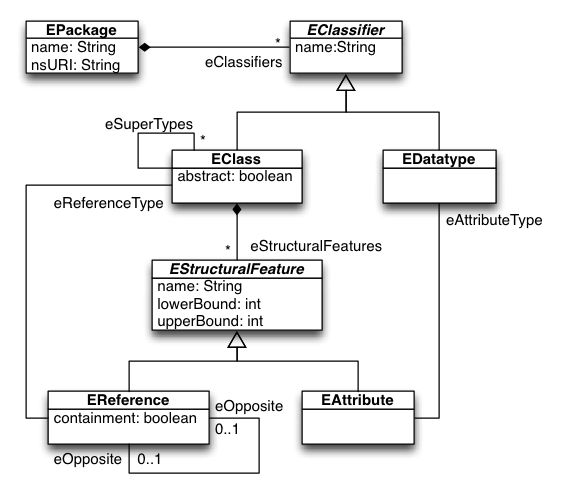
\includegraphics[width=.7\textwidth]{figures/ecore.png}
\caption{A small image, centered horizontally~\cite{ecore}.}
\label{fig:ecore}
\end{figure}

\begin{sidewaysfigure}
\centering
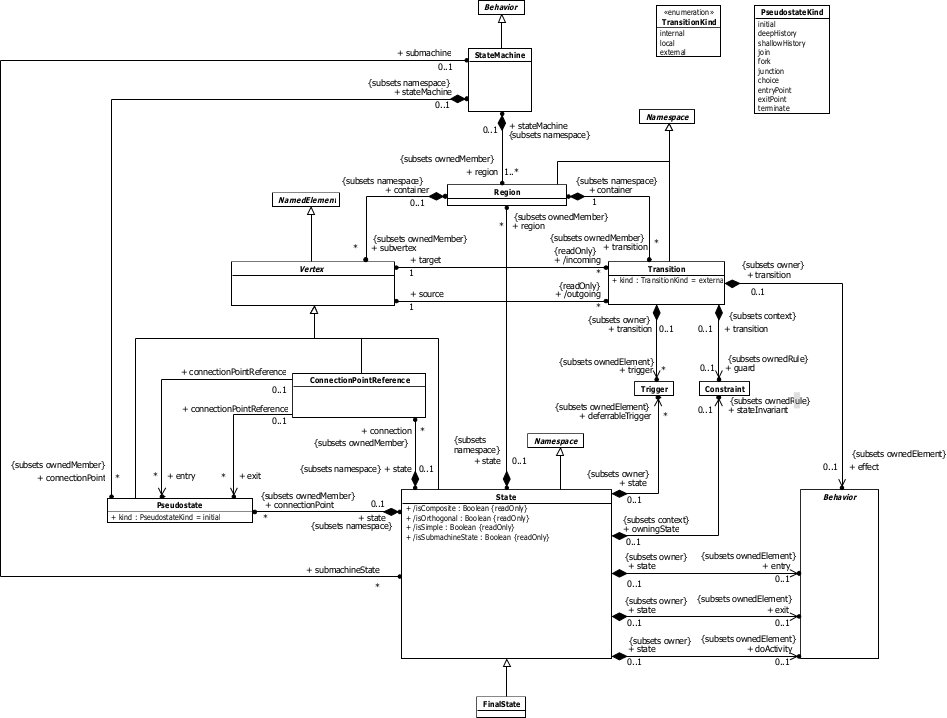
\includegraphics[width=\maxwidth{\textwidth}]{figures/omgfsm.png}
\caption{A wholepage image, rotated sideways~\cite{omguml}.}
\label{fig:omgfsm}
\end{sidewaysfigure}

\subsection{Diagrams}
It's also possible to draw diagrams \textit{inside} \LaTeX\ code.
\[
\begin{tikzcd}
L\arrow{d}{tr} = & (L^S \arrow{d}{tr^S} &   \arrow{l}{s_L}  L^C\arrow{d}{tr^C} \arrow{r}{t_L} & L^T \arrow{d}{tr^T}) \\
R = & (R^S & \arrow{l}{s_R} R^C \arrow{r}{t_R} & R^T)
\end{tikzcd}
\]

\clearpage
\subsection{Lists}
List for unordered things:
\begin{itemize}
\item Apple is a deciduous tree in the rose family best known for its sweet, pomaceous fruit, the apple.
\item Orange is the fruit of the citrus species Citrus $\times$ sinensis in the family Rutaceae. The fruit of the Citrus $\times$ sinensis is considered a sweet orange, whereas the fruit of the Citrus $\times$ aurantium is considered a bitter orange.
\item Pomegranate is a fruit-bearing deciduous shrub or small tree in the family Lythraceae that grows between 5 and 8 m tall.
\end{itemize}

Enumerated list for ordered things:
\begin{enumerate}
\item Open door.
\item Enter room.
\item Close door. 
\end{enumerate}

Named list for dictionary-like descriptions:
\begin{description}
\item[Apple] A deciduous tree in the rose family best known for its sweet, pomaceous fruit, the apple.
\item[Orange] The fruit of the citrus species Citrus $\times$ sinensis in the family Rutaceae. The fruit of the Citrus $\times$ sinensis is considered a sweet orange, whereas the fruit of the Citrus $\times$ aurantium is considered a bitter orange.
\item[Pomegranate] A fruit-bearing deciduous shrub or small tree in the family Lythraceae that grows between 5 and 8 m tall.
\end{description}

\subsection{Text formatting}
The usual text formatting options (\textbf{bold}, \textit{italic}, \texttt{fix-width}) are also available in \LaTeX. 
\begin{verbatim}
The verbatim environment can be used to
present multiline text with fix-width font.
\end{verbatim}

\clearpage
\subsection{Algorithm}
Below is an example usage of the algorithm environment. You can use this environment to include pseudocode in your thesis, usually to describe programs and algorithms you invented.


\algdef{SE}[DOWHILE]{Do}{doWhile}{\algorithmicdo}[1]{\algorithmicwhile\ #1}%
\begin{algorithm}
\footnotesize
\caption{$discoverGenFsm(modulName)$}         
\label{dfs}                           
\begin{algorithmic}[1]
  \State $ spgModel \leftarrow new SpgModel()$
  \State $ root \leftarrow new Root()$
  \State $ spgModel.setRoot(root) $
  \State $ modul \leftarrow new Modul(modulName) $
  \State $ root.addChild('mod', modul) $
  
  \For{$ f \in initFuns$ }
      \State $modul.addChild('func', erlNode2ModelNode(f))$
   \EndFor 

  \State $ visited \leftarrow new Set(initFuns) $
  \State $ stack \leftarrow new Stack(initFuns) $

  \State $ Visited \leftarrow Init$
  \State $S \leftarrow stack(V)$

  \While{ $stack \neq \varnothing$ } 
    \State $ node \leftarrow stack.pop()$

    \If {$v \not\in visited$}
      \State $ visited.add(node)$
      \State $ modelNode \leftarrow erlNode2ModelNode(node)$
      \State $ neighbours \leftarrow nextNode(node) $
      \For{$ (e,n) \in neighbours$ }
        \State $stack.add(n)$
        \State $modelNode.addChild(e, erlNode2ModelNode(node))$
      \EndFor 
    \EndIf
  \EndWhile    

  \Return $spgModel$
\end{algorithmic}
\end{algorithm}


\subsection{Source code}
Below is an example usage of the listings environment. You can use this environment to include source code in your thesis, usually to show source code examples.   

\begin{figure}[h]
\begin{lstlisting}[extendedchars=true, language=Erlang, basicstyle=\footnotesize\ttfamily, keywordstyle=\color{red}]
-module(hello). 
-export([hello_world/0]).

%% Outputs "hello world\n" on the standard output.
hello_world(ok) ->   
    X = "hello world\n",  
    io:fwrite(X); 

hello_world(_) ->  
   ok. 
\end{lstlisting}
\caption{A "Hello world" program in the Erlang language. Syntax highlighting is provided by the listings environment.}
\label{fig:helloworld}
\end{figure}

\subsection{Tables}
\begin{table}[!htb]
\centering
    \caption{Runtime test results}
    \label{tab:tests}
\noindent\adjustbox{max width=0.9\textwidth}{
    \begin{tabular}{|c|c|c|}
    \hline
    \textbf{Module}              & \textbf{Line no.}   & \textbf{Average (ms)}\\
    \hline
    \multicolumn{3}{|c|}{Ejabberd}                                            \\
    \hline
    ejabberd\_c2s                & 3128                & 31614.7              \\
    \hline                                                                    
    ejabberd\_service            & 404                 & 17991.3              \\
    \hline                                                                    
    eldap                        & 1196                & 27353.0              \\
    \hline                                                                    
    mod\_proxy65\_stream         & 291                 & 14975.9              \\
    \hline                                                                    
\multicolumn{3}{|c|}{Riak}                                                    \\
    \hline                                                                    
    riak\_kv\_2i\_aae            & 695                 & 11688.4              \\
    \hline                                                                    
    riak\_kv\_get\_fsm           & 787                 & 5521.9               \\
    \hline                                                              
\multicolumn{3}{|c|}{Erlang OTP}                                              \\
    \hline                                                              
    ssh\_connection\_handler     & 1721                & 67467.6              \\
    \hline                                                               
    tls\_connection              & 975                 & 56788.5              \\
    \hline
    \end{tabular}}
\end{table}



\chapter{Related Work}
\label{sec:related}

Since our goal is not the introduction of a new way to address the problem of creating correctness proofs for parallel programs, rather the adaptation of an existing system for formalized implementation, instead of discussing the theoretical methods, here we focus on a more practical approach and explore what others have achieved in the field of computer based verification.

\section{Previous works in Agda}
A very recent article \cite{Bergsten2017MethodsFU} presents an approach similar to ours, by setting out to provide an alternative to paper based proofs by formalizing an existing semi-formal model of concurrent programming. Their results provide methods for the confirmation of certain safety and liveness properties. Since it was the most closely related to what we have done, we compare their work to ours and discuss the similarities as well as the differences. The Agda programming language served as the meta-theory, in which the formalization and proofs were constructed for both projects, but the object-theory was different. We built our system around a language similar to UNITY, a language specifically created for and entirely based on parallelism for a book titled \textit{Parallel Program Design: A Foundation}\cite{misra1989foundation} (not to be confused with the modern game engine), that has essentially no guaranteed sequentiality, while their subject was an extension of the CPL language borrowed from \cite{owicki1982proving}, upon which they based most of their work, which is to some extent a regular imperative sequential language that has added constructs which introduce the capability for concurrency. This difference is also made very visible by their \textit{Proof by Control Flow} method, which implies that there is a distinct order present in the execution. Another big difference is the main focus of the projects. The aim for creating safety proofs was shared, but their other target, liveness proofs were not among our top priorities (although the fixed point property among our results can be related to it), rather we concentrated more on the formalization of general theorems as well as confirming adherence to specification, which is not included in their work. Further differences can be found by observing that the methods they utilize are in closer relation to operational semantics, while our formalization describes behavior in a manner more similar to denotational semantics. Also, some of the proofs presented in that paper are not completely constructive, some properties are only checked by functions essentially returning Boolean results, thus no so-called witness can be used for explaining or reasoning about the results, while the results that are presented in this current paper aim to all be constructive. They also did not implement every little detail included in their proofs, some steps include the usage of postulated properties, which are either relying on paper-based proofs or intuition. Our system is fully self-contained and is built from the ground up in a way meant not to include any external dependency. Their work was related to and part of it was further expanded in \cite{Johan2018ProofCF}.

\section{Previous works in Isabelle/HOL}
Another paper\cite{Complx-Isabelle} discusses a similar topic, but uses the Isabelle/HOL proof assistant\cite{nipkow2002isabelle} built on the imperative paradigm instead of the type theory based alternatives. Their main subject is a version of the generic SIMPL programming language originally introduced in \cite{simpl-schirmer2006verification}, that they extend in a way to support parallel composition and synchronization through shared-variable concurrency and called it COMPLEX. This still results in a system, which is sequential in its nature and contains concurrent sections. This approach is fitting for their goals, as one of their future aims is the translation of low level C code into COMPLEX for verification of for example concurrent operating system kernels. Their work is inspired by the Hoare-Parallel framework\cite{hoare-parallel-nieto2002verification} which is a formalization built using the Owicki-Gries method\cite{owicki1976axiomatic} in Isabelle/HOL. The Owicki-Gries method extends the verification procedure of sequential programs by introducing the notion of \textit{interference freedom}. It works by first proving each single thread correct on its own and then the atomic instructions of the threads are proven not to interfere with the correctness of each other.

\section{Previous works in Coq}
A case study\cite{coq-concurrent-verification-case-study} shows that there are many advantages to the library based approach, which eliminates some complicated modeling tasks by implementing a generalized version of parallelism instead of aiming straight for the proof of a concrete program. They investigate these properties through the verification procedure of a mail server originally written in Java by rewriting it in a modeling language provided by a library. \cite{coq-mail-server} The development of the Coq library is discussed in \cite{AFFELDT200817}. It contains a modeling language based on $\pi$-calculus
% \cite{pi-calculus-Milner1992ACO}
\cite{MILNER19921}
\cite{MILNER199241}
\cite{sangiorgi2003pi}
(which has been modified to enable the usage of Coq datatypes and control structures), a specification language and a collection of reusable lemmas. In this sense, it is similar to our approach, as these mentioned components are also present among our results. Models formalized in their library are also suitable for extraction into executable OCaml code using the facilities provided by Coq, although it is not fully automatic and requires manual modifications.

Another paper based in Coq \cite{Heyd1996AMC} is closely related to our work in the sense, that it takes the UNITY theoretical programming language as its subject of formalization, the same system on top of which the material of the course discussed later is based on. Their approach is much more abstract, as they are only constraining elements to functions between certain types, not limiting them to be created by an established set of constructors. Also, they do not discuss conditions at all. Compared to this, while being less general, our results are much more approachable, since they are built using inductive types that not only give constructing blocks for programs and predicates, but also serve as stricter and stronger guiding outlines to aid the development of proofs about the system.

\section{Our work}
Our approach is different from these examples in that its main goal is to aid the development of solutions given through the formalized specification language, not necessarily the verification of already existing codebases. The control flow (or more like the lack thereof) is also a big differentiation factor of our model when comparing to other similar systems.

\section{Proof assistant for parallel systems}
In another article\cite{Mauw1991APA}, that is more on the theoretical side, but we still considered relevant, the description of a proof assistant based on the algebra of communicating processes, specifically designed for proofs around parallel systems is given.



% In \cite{proving-parallel-assertions} we can see the application of such methods to a concrete program, several properties of an elementary airline reservation system implemented in a general parallel programming language are verified.

% TODO: min. 2 oldal

\label{chp:related}

\chapter{Background}
\label{chp:background}

In the following chapter we introduce the material that we based our formalization on and the system we chose as our meta-theory. We do not cover the whole model in detail, but mostly focus on the concepts that are needed for understanding the results of our work. A short introduction to Agda, the language of our choice can also be found at the end of the chapter.

\section{Subject: Specification and Implementation of Distributed Systems}
\label{sec:subject}

The subject of our formalization is a part of the material from the \textit{Specification and Implementation of Distributed System} course taught at ELTE. The main goal was following the official notes of the subject\cite{hz-orsi} as closely as possible, but since the code needed to be more precise than written definitions, some constructs were altered. The system extends a relational model defined in \cite{fothi-prog} which itself is built upon Hoare-logic \cite{hoare1978proof}\cite{hoare-logic}, more specifically concurrent Hoare-logic\cite{Lamport1980}. Proofs for sequential programs are handled using pre- and postconditions with the devices provided by first order logic. This is expanded to parallel execution in a similar fashion to UNITY. Abstract programs are formalized through a set of conditional assignments the execution of which are represented as a list of state transitions that can be considered as trees, which results in a branching-time temporal logic \cite{emerson1988branching} (more specifically computation tree logic) like system.

An abstract program as defined by this system can be thought of as an initialization and a set of further conditional instructions. These are then selected randomly and if their condition is satisfied in the current program state, they are executed. This can be done in any arbitrary order, their behaviour stays the same if the scheduling is impartial. The execution units running such a program can be thought of as processing cores, or even several computers working together in a cluster.

\begin{definition}{Interleaving semantics}
\label{def:interleaving-semantics}
In a model that conforms to interleaving semantics, for every valid parallel execution, there also exists a linear execution path of the same instructions, that achieves equivalent results.
\end{definition}

\begin{definition}{Impartial Scheduling}
\label{def:impartial-scheduling}
A scheduling is called impartial if it ensures that running the program indefinitely will result in the selection of each and every conditional instruction infinitely many times.
\end{definition}

After laying down the foundation for constructing programs and reasoning about their behavior, the subject introduces a formal concept of task specification and then defines the correctness of a program by proving that it adheres to those constraints posed by the specification. We iterate on these constructions and implement them, so the verification of the adherence can be done on the computer, thus avoiding potential human errors that can occur while carrying out such a process on paper.

There are multiple ways, in which said correctness of a program can be shown. Simply giving a proof, that all the imposed criteria are held is always sufficient, but gets inconvenient for larger programs. To avoid the complication of proofs, one can utilize the method of reduction to an already known problem. If there is a recurring pattern, general statements about its behavior can be proven, so that these do not need to be done each and every time the pattern is used. Just showing how the currently examined part of the program corresponds to the pattern is enough instead. Another technique for avoiding repetition and introducing segmentation into proofs to keep their brevity is to construct programs from other smaller programs, by for example taking their union, essentially using them as so called \textit{building blocks}.

\subsection[Mathematical foundation]{Mathematical foundation\protect\footnote{The original model is more general than the one described here, but since our formalization uses functions, that are deterministic, we constrained the ranges of some relations to single values instead of sets.}}

The basics of the material are built on top of a relational model, the development of which originates from the works of Ákos Fóthi\cite{fothi1988mathematical}. This model deals with programs, that operate over a so called \textbf{state space}, which is built as a Cartesian product of the individual sets of possible values for the variables of the program: $A = A_1 \times A_2 \times \ldots \times A_n$. These sets are individually called \textbf{type value sets}. The value of a single variable in a certain state can be accessed by the projection function $v_i : A \to A_i$.

Let $A^*$ denote the finite and $A^\infty$ the infinite sequences made of elements in $A$. The set of all sequences with elements from $A$, that can either be finite or infinite is defined as $A^{**} = A^* \cup A^\infty$.

We call a function a \textit{logical function}, if it maps into the set of Boolean logical values defined as $\mathbb{B} = {true , false}$. A subset of these functions, that not only have $\mathbb{B}$ as their range, but also a state space $A$ as their domain can be called conditions. These have the type $\pi : A \to \mathbb{B}$.

\begin{definition}{Truth set}
\label{def:truth-set}
The subset of the state space in which these conditions are satisfied is often of interest, for this purpose the notion of the \textbf{truth set} of a function is defined as the subset of its domain that it maps to $true$. It is denoted as follows: $\lceil \pi \rceil = \{a \in A \;|\; \pi(a) = true\}$
\end{definition}

\begin{definition}{Implication}
\label{def:implication}
One condition is said to imply another ($P \Rightarrow Q$) if its truth set is subset of the others ($\lceil P \rceil \subset \lceil Q \rceil$).
\end{definition}

Another specific kind of function that operates on states is the so called \textbf{state transition function}. It has the type signature of $A \to A$ and is used to describe the behavior of an instruction. In this model, we consider only a single kind of instruction, namely a generic type of assignment, which is defined in the following way. Given a function for every variable index of the state space, that maps from the entire state space to the type value set of that given variable ($\forall i \in \{1..n\} : F_i : A \to A_i$), combining these into a single function $F = (F_1, \ldots F_n)$ we get a state transition function. Semantically speaking, it describes a parallel assignment, where each variable can have a formula, that may depend on all the other variables (or itself as well), these then are evaluated in the same state and get their new values assigned concurrently to produce a new, updated state.

Such an assignment can be made conditional by pairing it with a logical function. By doing so, we alter its state transition function in a way, that it only applies the changes to the state, if its condition is fulfilled (meaning, that the current state is in its truth set), otherwise it acts as an identity function. With mathematical notation, given $\pi : A \to \mathbb{B}$ as a condition and $F : A \to A$ as an assignment, we get the following conditional state transition function:

\begin{equation}
    F'(a) = 
    \left\{
    	\begin{array}{ll}
    		F(a) & \mbox{if } a \in \lceil \pi \rceil \\
    		a & \mbox{otherwise}
    	\end{array}
    \right.
\end{equation}

A parallel program ($S = (s_0, \{s_1, \ldots, s_m\})$) defined using these constructs consists of a single initialization assignment and a set of conditional assignments to be repeatedly performed later in no particular order. Any requirements that would be posed for their sequentiality need to be encoded into their conditions, which in turn can ensure some sort of a control flow. A parallel program constructed in such a way can be semantically thought of as a relation that maps any state to a branching series of possible successive states (see Figure \ref{fig:branching-execution} as an illustration). If we remove the successively duplicated states from these series by replacing all consecutive repetitions of a single state with only one instance, we get their so-called \textit{reduced} versions. This gives us the type signature $A \times A^{**}$, meaning that for any given state, the program determines the set of possible execution paths, which are either finite (if a program terminates by reaching a fixed point) or infinite (that might represent a continuously running server) series of states.

\begin{figure}[H]
    \centering
    \usetikzlibrary{trees}
% \tikzstyle{level 1}=[level distance=2cm, sibling distance=4cm]
% \tikzstyle{level 2}=[level distance=2cm, sibling distance=1cm]
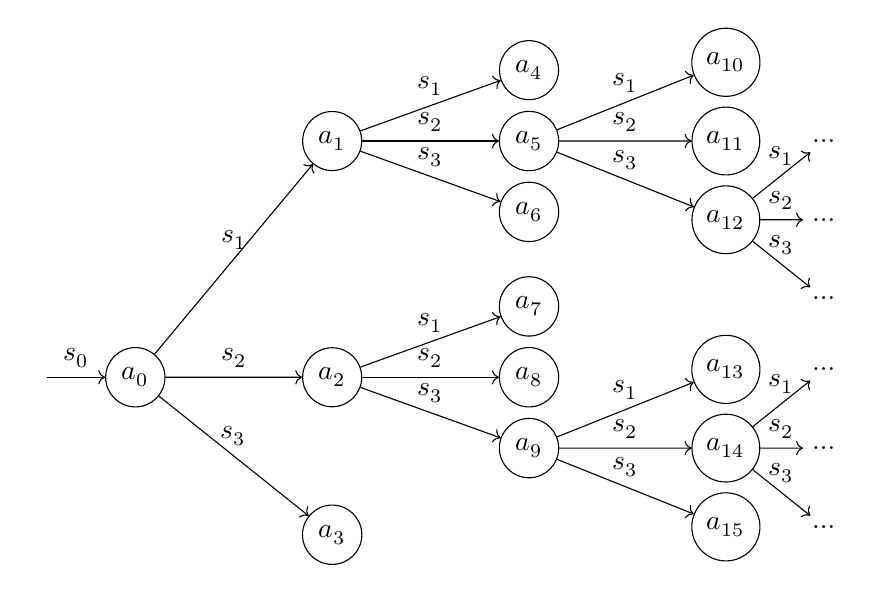
\begin{tikzpicture}[
        grow=right,
        ->,
        % every node/.style={draw,circle},
        state/.style={draw, circle},
        % treenode/.style = {circle, white, draw=black, align=center, inner sep=0pt, text centered, font=\sffamily},
        % thick,
        % Set the overall layout of the tree
        level/.style={level distance=2.5cm},
        level 1/.style={level distance=1.25cm},
        level 2/.style={sibling distance=3cm},
        level 3/.style={sibling distance=0.9cm},
        level 4/.style={sibling distance=1cm},
        level 5/.style={level distance=1.25cm},
        % level/.style={sibling distance = 5cm/#1, level distance = 1.5cm}
    ]
    \node {}
    child {
        node [state] {$a_0$}
        child [sibling distance=2cm] {
            node [state] {$a_3$}
            edge from parent node [above] {$s_3$}
        }
        child {
            node [state] {$a_2$}
            child {
                node [state] {$a_9$}
                child {
                    node [state] {$a_{15}$}
                    edge from parent node [above] {$s_3$}
                }
                child {
                    node [state] {$a_{14}$}
                    child {
                        node {$\ldots$}
                        edge from parent node [above] {$s_3$}
                    }
                    child {
                        node {$\ldots$}
                        edge from parent node [above] {$s_2$}
                    }
                    child {
                        node {$\ldots$}
                        edge from parent node [above] {$s_1$}
                    }
                    edge from parent node [above] {$s_2$}
                }
                child {
                    node [state] {$a_{13}$}
                    edge from parent node [above] {$s_1$}
                }
                edge from parent node [above] {$s_3$}
            }
            child {
                node [state] {$a_8$}
                edge from parent node [above] {$s_2$}
            }
            child {
                node [state] {$a_7$}
                edge from parent node [above] {$s_1$}
            }
            edge from parent node [above] {$s_2$}
        }
        child {
            node [state] {$a_1$}
            child {
                node [state] {$a_6$}
                edge from parent node [above] {$s_3$}
            }
            child {
                node [state] {$a_5$}
                child {
                    node [state] {$a_{12}$}
                                        child {
                        node {$\ldots$}
                        edge from parent node [above] {$s_3$}
                    }
                    child {
                        node {$\ldots$}
                        edge from parent node [above] {$s_2$}
                    }
                    child {
                        node {$\ldots$}
                        edge from parent node [above] {$s_1$}
                    }
                    edge from parent node [above] {$s_3$}
                }
                child {
                    node [state] {$a_{11}$}
                    edge from parent node [above] {$s_2$}
                }
                child {
                    node [state] {$a_{10}$}
                    edge from parent node [above] {$s_1$}
                }
                edge from parent node [above] {$s_2$}
            }
            child {
                node [state] {$a_4$}
                edge from parent node [above] {$s_1$}
            }
            edge from parent node [above] {$s_1$}
        }
        edge from parent node [above] {$s_0$}
    };
\end{tikzpicture}

% \begin{tikzpicture}[
%         ->,
%         every node/.style={draw,circle},
%         % treenode/.style = {circle, white, draw=black, align=center, inner sep=0pt, text centered, font=\sffamily},
%         thick,
%         % Set the overall layout of the tree
%         level/.style={level distance=1.5cm},
%         level 2/.style={sibling distance=2.6cm},
%         level 3/.style={sibling distance=2cm}
%     ]
%     \coordinate
%         child[grow=left]{
%             node {$a_0$}
%             % node [treenode] {$a_0$}
%             edge from parent node [above=3pt] {$s_0$}
%         }
%         % I have to insert a dummy child to get the tree to grow
%         % correctly to the right.
%         child[grow=right, level distance=0pt] {
%         node [above] {$a_1$}
%         child  {
%             child {
%                 child {
%                     node {$\bar{d}$}
%                     edge from parent
%                 }
%                 child {
%                     node {$u$}
%                     edge from parent
%                 }
%                 edge from parent
%             }
%             child {
%                 node {$b$}
%                 edge from parent
%             }
%             edge from parent
%             node [below] {$t$}
%         }
%         child {
%             child {
%                 node {$\bar{b}$}
%                 edge from parent
%             }
%             child {
%                 child {
%                     node {$\bar{v}$}
%                     edge from parent
%                 }
%                 child {
%                     node {$e^{-}$}
%                     edge from parent
%                 }
%                 edge from parent
%             }
%             edge from parent
%             node [above] {$\bar{t}$}
%         }
%     };
% \end{tikzpicture}
    \caption{Branching execution with possible paths, e.g., $(a_0,a_2,a_9,a_{15})$, $(a_0,a_1,a_5,a_{12},...)$.}
    \label{fig:branching-execution}
\end{figure}

By constructing a type of specification that only places constraints on states, we can achieve independence from the actual structure of programs operating on these states. Problems consist of seven so called \textit{Specification Properties}, which are themselves given as relations over the power set of the state space. These provide constraints for the behavior of the program, that will eventually have to satisfy all of them to be considered adherent to the specification and thus solve the problem.

Let $P, Q : A \to \mathbb{B}$, the infix notation $P \Circle Q$ mean $(\lceil P
\rceil , \lceil Q \rceil) \in \Circle$, where $\Circle$ is any of the binary
relations $\rhd, \mapsto, \hookrightarrow$ and for the unary relations $\CIRCLE
\in \{FP, INIT, inv, TERM\}$, let $P \in \CIRCLE$ mean $\lceil P \rceil \in
\CIRCLE$

% They can be classified into four groups:
% Safety properties:
% Progress properties:
Let the following specification properties be proposed:
\begin{itemize}
    \item $\rhd \in \mathcal{P}(\mathcal{P}(A) \times \mathcal{P}(A))$, where $P \rhd Q$ means, that leaving $\lceil P \rceil$ requires going through $\lceil Q \rceil$
    % the truth set of predicate $P$ can only be left by going through the truth set of $Q$
    \item $\mapsto \in \mathcal{P}(\mathcal{P}(A) \times \mathcal{P}(A))$, where $P \mapsto Q$ extends upon $P \rhd Q$ by stating that $\lceil P \rceil$ can indeed be left through $\lceil Q \rceil$, and only through it
    \item $\hookrightarrow \in \mathcal{P}(\mathcal{P}(A) \times
      \mathcal{P}(A))$, where $P \hookrightarrow Q$ states that from every state in the truth set of $P$ we must eventually get to a point in the truth set of $Q$ (formally it is the transitive disjunctive closure (see Definition
      \ref{def:transitive-disjunctive-closure}) of $\mapsto$)
    \item $FP \subseteq \mathcal{P}(A)$ where $P \in FP$ means that if the program has reached a fixed point (meaning, that it can make no further state transitions), then $P$ must be satisfied
    \item $INIT \subseteq \mathcal{P}(A)$, where $P \in INIT$ means that the predicate $P$ is satisfied at the beginning of the program
    \item $inv \subseteq \mathcal{P}(A)$, where $P \in inv$ means that $P$ is satisfied at the beginning of the program and once its truth set has been entered, it cannot be left, thus it is an invariant for the entire program
    \item $TERM \subseteq \mathcal{P}(A)$, where $P \in TERM$ means that after the program has entered the truth set of $P$, it is guaranteed to eventually reach a fixed point
\end{itemize}

\begin{definition}{Transitive Disjunctive Closure}
\label{def:transitive-disjunctive-closure}
The transitive disjunctive closure of a relation $R \subset (A \times A)$, where $\lor : A \to A \to A$ is given as the binary disjunction operator, is denoted by $R^{tdl} \subset (A \times A)$. It is defined as the minimal relation with the following properties.
\begin{itemize}
    \item It is a superset of the original relation ($R \subset R^{tdl}$).
    \item Transitivity: For every ($a, b, c \in A$) if $(a, b) \in R^{tdl}$ and $(b, c) \in R^{tdl}$, then $(a, c) \in R^{tdl}$ as well.
    \item Disjunctivity: For every ($a, b, c \in A$) if $(a, c) \in R^{tdl}$ and $(b, c) \in R^{tdl}$, then $(a \lor b) \in R^{tdl}$ as well.
\end{itemize}
\end{definition}

A tuple with seven items, each describing elements from one of the relations given above, can be considered as a specification for a program. If a parallel program satisfies all the constraints posed by a specification, it is considered to be a solution for the given problem.

% A program for solving problems defined by such specifications can be constructed as a set of conditional assignments. A generic conditional assignment is defined as a function that maps states to states. Its behavior can be defined as a function that checks whether a certain requirement is satisfied in the current state, and if it is, then it assigns new values to the variables of the state space.

% TODO: Lamsweerde Sintzoff


%% Behavior relation
%% Parameter space
%% Solution


\section{Type Theory}
In the following section we will discuss what Type Theory is, how it enables formalization of models with proofs, to be checked by computers and explain our choice of the Agda implementation.

\subsection{General Principles Overview}

Type theory is an alternative foundation for mathematics, which enables the formalization of constructive proofs through the connections to intuitionistic logic given by the Brouwer–Heyting–Kolmogorov interpretation. After formalizing a model by defining its types and their elements, one can express statements and theorems in forms of new types, the instances of which can be thought as of proofs for them.
This is due to the so called \textit{"propositions-as-types"} paradigm, formally known as the Curry–Howard isomorphism.

As an example, given two statements, $A$ and $B$, the function with the type signature $A \to B$ represents the theorem which claims that every proof of $A$ can be mapped to a proof for $B$, thus $A$ ensures $B$. If an implementation for a function with said type is given, the theorem can be considered the be proven, since if we are in possession of a proof for $A$, we can execute it and obtain a proof for $B$. The fact that it does not only claim, that such an instance exists, but gives one right away instead is called a constructive proof.

\subsection{Implementations}
There are several existing programming languages that implement type theories, thus are capable of describing theorems and constructing proofs for them. They achieve this using dependent typesystems, in which types can not only be parametrized over other types, but also values. Out of these we tried out the three most popular alternatives.

\subsubsection{Idris}
Idris\cite{Brady2013IdrisAG} is a relatively new contender in the field of programming with dependent types. Its development is led by Edvin Brady with the aim of creating a general purpose language.

We first tried implementing our formalisation in Idris, as it seemed to be the freshest language. It also has good support for every major operating system, wider editor compatibility than the alternatives and in some sense a more modern standard library, which is easier to discover due to the in our opinion better documentation.

Under certain circumstances the implicit parameter handling of Idris seemed to better for us than that of Agda, and there are constructs, such as for example heterogeneous vectors that are easier to implement in Idris, because it uses cumulative universes, but
after reaching a certain complexity, the type checker of Idris unfortunately turned out to be too slow, so we moved on to other languages. It also lacks Unicode support, with perfectly valid and understandable reasons outlined by Edvin Brady, but it also makes the code a lot more verbose and harder to integrate with the original notation.

% ?Idris also has heterogeneous vectors which are harder to create in Agda due to its implementation of universe polymorphism.?


\subsubsection{Agda}
Agda is a dependently typed programming language that was originally described in the PhD thesis of Ulf Norell\cite{norell:thesis} and later completely rewritten for a second version. It mainly follows the style of Haskell.

Its conventions of highly relying on Unicode symbols for identifiers helped in staying similar to the original notation of the curriculum of the subject.

\subsubsection{Coq}
The Coq proof assistant\cite{} is the earliest of the three, even predating Agda by ten years. (The initial version was released on the 1st of May, 1989.) It is really well established and focuses mainly on creating proofs using a tactic language instead of using regular functional programming constructs.

\chapter{Method}

Our approach started with an implementation of a highly simplified model in Idris, that served as an initial proof-of-concept. The development process was done in an iterative style, meaning that we had to backtrack multiple times and rewrite certain parts over and over, but this often helped in finding better solutions. Some simple proofs were written in Idris, but after trying to expand to a more complex model, the type checking of Idris seemed to be too slow, which led to the decision of switching to Agda.



\chapter{Results}
\label{chp:results}

In this chapter we discuss the different kind of outcomes we have currently arrived at, explain how they are build and illustrate them with samples from the source code.

\section{Formalization}

In this section we present our formalization of the notion of parallel programs, predicates and their semantics introduced by the model we build upon. The formalization of a parallel bubble sort and the concepts that are required for writing specification statements are also included.

\subsection{Parallel Programs and Predicates}

Since our formalization does not follow the book of the subject exactly, we present the following basic notions that we introduced in our version and built upon:
\begin{itemize}
    \item \verb|Type| - We defined the set of possible types of variables in the programs as an inductive datatype, which enabled the use of parametric types as well.
    \begin{code}
        \>[0]\AgdaKeyword{data}\AgdaSpace{}%
        \AgdaDatatype{Types}\AgdaSpace{}%
        \AgdaKeyword{where}\<%
        \\
        \>[0][@{}l@{\AgdaIndent{0}}]%
        \>[2]\AgdaInductiveConstructor{Nat}\AgdaSpace{}%
        \AgdaSymbol{:}\AgdaSpace{}%
        \AgdaDatatype{Types}\<%
        \\
        %
        \>[2]\AgdaInductiveConstructor{Array}\AgdaSpace{}%
        \AgdaSymbol{:}\AgdaSpace{}%
        \AgdaDatatype{Types}\AgdaSpace{}%
        \AgdaSymbol{→}\AgdaSpace{}%
        \AgdaDatatype{Types}\<%
        \\
        %
        \>[2]\AgdaInductiveConstructor{DataChannel}\AgdaSpace{}%
        \AgdaSymbol{:}\AgdaSpace{}%
        \AgdaDatatype{Types}\AgdaSpace{}%
        \AgdaSymbol{→}\AgdaSpace{}%
        \AgdaDatatype{Types}\<%
    \end{code}
    
    \item \verb|Environment| - An environment has a defined number of variables and a type assigned to each of them. It essentially describes a state space. (The type \verb|Fin n| denotes the finite set with $n$ elements, see Appendix \ref{apx:codes} for its definition.)
    \begin{code}
        \>[0]\AgdaKeyword{module}\AgdaSpace{}%
        \AgdaModule{Environment}\AgdaSpace{}%
        \AgdaSymbol{(}\AgdaBound{varCount}\AgdaSpace{}%
        \AgdaSymbol{:}\AgdaSpace{}%
        \AgdaDatatype{ℕ}\AgdaSymbol{)}\AgdaSpace{}%
        \AgdaSymbol{(}\AgdaBound{varTypes}\AgdaSpace{}%
        \AgdaSymbol{:}\AgdaSpace{}%
        \AgdaDatatype{Fin}\AgdaSpace{}%
        \AgdaBound{varCount}\AgdaSpace{}%
        \AgdaSymbol{→}\AgdaSpace{}%
        \AgdaDatatype{Types}\AgdaSymbol{)}\AgdaSpace{}%
        \AgdaKeyword{where}\<%
    \end{code}
    
    \item \verb|Variable| - A variable in this model can be thought of as just an index, that can be used to reference a certain part of the state.
    \begin{code}
        \>[2]\AgdaFunction{Vars}\AgdaSpace{}%
        \AgdaSymbol{:}\AgdaSpace{}%
        \AgdaPrimitiveType{Set}\<%
        \\
        %
        \>[2]\AgdaFunction{Vars}\AgdaSpace{}%
        \AgdaSymbol{=}\AgdaSpace{}%
        \AgdaDatatype{Fin}\AgdaSpace{}%
        \AgdaBound{varCount}\<%
    \end{code}
    
    \item \verb|State| - We modeled a state as a function that maps the previously introduced variables to the respective value sets of their types. (The \verb|evaluateType| function assigns the previously defined data types to their Agda representations. It has multiple possible definitions which can all be equivalent in terms of the expressive power of the resulting model, what it affects is the structure of the proofs. A possible definition we used can be found in appendix \ref{apx:codes}.)
    \begin{code}
        \>[2]\AgdaFunction{State}\AgdaSpace{}%
        \AgdaSymbol{:}\AgdaSpace{}%
        \AgdaPrimitiveType{Set}\<%
        \\
        %
        \>[2]\AgdaFunction{State}\AgdaSpace{}%
        \AgdaSymbol{=}\AgdaSpace{}%
        \AgdaSymbol{(}\AgdaBound{i}\AgdaSpace{}%
        \AgdaSymbol{:}\AgdaSpace{}%
        \AgdaFunction{Vars}\AgdaSymbol{)}\AgdaSpace{}%
        \AgdaSymbol{→}\AgdaSpace{}%
        \AgdaFunction{evaluateType}\AgdaSpace{}%
        \AgdaSymbol{(}\AgdaBound{varTypes}\AgdaSpace{}%
        \AgdaBound{i}\AgdaSymbol{)}\<%
    \end{code}
    
    \item \verb|Expression| - The building blocks that can be used for constructing an expression that can either be on the right hand side of an assignment or serve as a part of a predicate. They are annotated with the types that are the results of their evaluation, which increases the potential for code reuse by eliminating the need for separate constructors for separate types and prevents their usage in the wrong contexts.
    \begin{code}
        \>[2]\AgdaKeyword{data}\AgdaSpace{}%
        \AgdaDatatype{Expression}\AgdaSpace{}%
        \AgdaSymbol{:}\AgdaSpace{}%
        \AgdaDatatype{Types}\AgdaSpace{}%
        \AgdaSymbol{→}\AgdaSpace{}%
        \AgdaPrimitiveType{Set}\AgdaSpace{}%
        \AgdaKeyword{where}\<%
    \end{code}
    \begin{itemize}
        \item The \verb|Const| constructor creates a constant expression by directly giving the Agda representation of its value.
        \begin{code}
            % \>[2][@{}l@{\AgdaIndent{0}}]%
            \>[4]\AgdaInductiveConstructor{Const}\AgdaSpace{}%
            \AgdaSymbol{:}\AgdaSpace{}%
            \AgdaSymbol{\{}\AgdaBound{A}\AgdaSpace{}%
            \AgdaSymbol{:}\AgdaSpace{}%
            \AgdaDatatype{Types}\AgdaSymbol{\}}\AgdaSpace{}%
            \AgdaSymbol{→}\AgdaSpace{}%
            \AgdaFunction{evaluateType}\AgdaSpace{}%
            \AgdaBound{A}\AgdaSpace{}%
            \AgdaSymbol{→}\AgdaSpace{}%
            \AgdaDatatype{Expression}\AgdaSpace{}%
            \AgdaBound{A}\<%
        \end{code}
        
        \item The \verb|GetArray| constructor creates an expression that accesses a value at a specific index from an array.
        \begin{code}
            \>[4]\AgdaInductiveConstructor{GetArray}\AgdaSpace{}%
            \AgdaSymbol{:}\AgdaSpace{}%
            \AgdaSymbol{\{}\AgdaBound{A}\AgdaSpace{}%
            \AgdaSymbol{:}\AgdaSpace{}%
            \AgdaDatatype{Types}\AgdaSymbol{\}}\AgdaSpace{}%
            \AgdaSymbol{→}\<%
            \\
            \>[4][@{}l@{\AgdaIndent{0}}]%
            \>[6]\AgdaDatatype{Expression}\AgdaSpace{}%
            \AgdaInductiveConstructor{Nat}\AgdaSpace{}%
            \AgdaSymbol{→}\AgdaSpace{}%
            \AgdaDatatype{Expression}\AgdaSpace{}%
            \AgdaSymbol{(}\AgdaInductiveConstructor{Array}\AgdaSpace{}%
            \AgdaBound{A}\AgdaSymbol{)}\AgdaSpace{}%
            \AgdaSymbol{→}\AgdaSpace{}%
            \AgdaDatatype{Expression}\AgdaSpace{}%
            \AgdaBound{A}\<%
        \end{code}
        
        \item The \verb|SetArray| constructor creates an expression that creates a modified version of a given array, that contains an updated value at the given index.
        \begin{code}
            \>[4]\AgdaInductiveConstructor{SetArray}\AgdaSpace{}%
            \AgdaSymbol{:}\AgdaSpace{}%
            \AgdaSymbol{\{}\AgdaBound{A}\AgdaSpace{}%
            \AgdaSymbol{:}\AgdaSpace{}%
            \AgdaDatatype{Types}\AgdaSymbol{\}}\AgdaSpace{}%
            \AgdaSymbol{→}\<%
            \\
            \>[4][@{}l@{\AgdaIndent{0}}]%
            \>[6]\AgdaDatatype{Expression}\AgdaSpace{}%
            \AgdaInductiveConstructor{Nat}\AgdaSpace{}%
            \AgdaSymbol{→}\AgdaSpace{}%
            \AgdaDatatype{Expression}\AgdaSpace{}%
            \AgdaBound{A}\AgdaSpace{}%
            \AgdaSymbol{→}\AgdaSpace{}%
            \AgdaDatatype{Expression}\AgdaSpace{}%
            \AgdaSymbol{(}\AgdaInductiveConstructor{Array}\AgdaSpace{}%
            \AgdaBound{A}\AgdaSymbol{)}\AgdaSpace{}%
            \AgdaSymbol{→}\<%
            \\
            %
            \>[6]\AgdaDatatype{Expression}\AgdaSpace{}%
            \AgdaSymbol{(}\AgdaInductiveConstructor{Array}\AgdaSpace{}%
            \AgdaBound{A}\AgdaSymbol{)}\<%
        \end{code}
        
        \item The \verb|Var| constructor creates an expression, the result of which is the value of a given variable in the state it is evaluated in.
        \begin{code}
            \>[4]\AgdaInductiveConstructor{Var}\AgdaSpace{}%
            \AgdaSymbol{:}\AgdaSpace{}%
            \AgdaSymbol{(}\AgdaBound{x}\AgdaSpace{}%
            \AgdaSymbol{:}\AgdaSpace{}%
            \AgdaFunction{Vars}\AgdaSymbol{)}\AgdaSpace{}%
            \AgdaSymbol{→}\AgdaSpace{}%
            \AgdaDatatype{Expression}\AgdaSpace{}%
            \AgdaSymbol{(}\AgdaBound{varTypes}\AgdaSpace{}%
            \AgdaBound{x}\AgdaSymbol{)}\<%
        \end{code}
        
        \item The expressions created by the \verb|Plus| constructor evaluate to the sum of what its subexpressions evaluate to.
        \begin{code}
            \>[4]\AgdaInductiveConstructor{Plus}\AgdaSpace{}%
            \AgdaSymbol{:}\AgdaSpace{}%
            \AgdaDatatype{Expression}\AgdaSpace{}%
            \AgdaInductiveConstructor{Nat}\AgdaSpace{}%
            \AgdaSymbol{→}\AgdaSpace{}%
            \AgdaDatatype{Expression}\AgdaSpace{}%
            \AgdaInductiveConstructor{Nat}\AgdaSpace{}%
            \AgdaSymbol{→}\AgdaSpace{}%
            \AgdaDatatype{Expression}\AgdaSpace{}%
            \AgdaInductiveConstructor{Nat}\<%
        \end{code}
        
        \item The \verb|Hiext| constructor allows for the creation of expressions that evaluate to an extended version of a given channel that has a new value added to it. This is more commonly called the \textit{enqueue} operation.
        \begin{code}
            \>[4]\AgdaInductiveConstructor{Hiext}\AgdaSpace{}%
            \AgdaSymbol{:}\AgdaSpace{}%
            \AgdaSymbol{\{}\AgdaBound{A}\AgdaSpace{}%
            \AgdaSymbol{:}\AgdaSpace{}%
            \AgdaDatatype{Types}\AgdaSymbol{\}}\AgdaSpace{}%
            \AgdaSymbol{→}\<%
            \\
            \>[4][@{}l@{\AgdaIndent{0}}]%
            \>[6]\AgdaDatatype{Expression}\AgdaSpace{}%
            \AgdaBound{A}\AgdaSpace{}%
            \AgdaSymbol{→}\AgdaSpace{}%
            \AgdaDatatype{Expression}\AgdaSpace{}%
            \AgdaSymbol{(}\AgdaInductiveConstructor{DataChannel}\AgdaSpace{}%
            \AgdaBound{A}\AgdaSymbol{)}\AgdaSpace{}%
            \AgdaSymbol{→}\AgdaSpace{}%
            \AgdaDatatype{Expression}\AgdaSpace{}%
            \AgdaSymbol{(}\AgdaInductiveConstructor{DataChannel}\AgdaSpace{}%
            \AgdaBound{A}\AgdaSymbol{)}\<%
        \end{code}
        
        \item The \verb|Lov| constructor creates an expression that accesses the first value in a given channel. This is more commonly called the \textit{peek} operation.
        \begin{code}
            \>[4]\AgdaInductiveConstructor{Lov}\AgdaSpace{}%
            \AgdaSymbol{:}\AgdaSpace{}%
            \AgdaSymbol{\{}\AgdaBound{A}\AgdaSpace{}%
            \AgdaSymbol{:}\AgdaSpace{}%
            \AgdaDatatype{Types}\AgdaSymbol{\}}\AgdaSpace{}%
            \AgdaSymbol{→}\AgdaSpace{}%
            \AgdaDatatype{Expression}\AgdaSpace{}%
            \AgdaSymbol{(}\AgdaInductiveConstructor{DataChannel}\AgdaSpace{}%
            \AgdaBound{A}\AgdaSymbol{)}\AgdaSpace{}%
            \AgdaSymbol{→}\AgdaSpace{}%
            \AgdaDatatype{Expression}\AgdaSpace{}%
            \AgdaBound{A}\<%
        \end{code}
        
        \item The \verb|Lorem| constructor creates an expression that evaluates to an updated version of a given channel, that has its first element removed. This is more commonly called the \textit{dequeue} operation.
        \begin{code}
            \>[4]\AgdaInductiveConstructor{Lorem}\AgdaSpace{}%
            \AgdaSymbol{:}\AgdaSpace{}%
            \AgdaSymbol{\{}\AgdaBound{A}\AgdaSpace{}%
            \AgdaSymbol{:}\AgdaSpace{}%
            \AgdaDatatype{Types}\AgdaSymbol{\}}\AgdaSpace{}%
            \AgdaSymbol{→}\<%
            \\
            \>[4][@{}l@{\AgdaIndent{0}}]%
            \>[6]\AgdaDatatype{Expression}\AgdaSpace{}%
            \AgdaSymbol{(}\AgdaInductiveConstructor{DataChannel}\AgdaSpace{}%
            \AgdaBound{A}\AgdaSymbol{)}\AgdaSpace{}%
            \AgdaSymbol{→}\AgdaSpace{}%
            \AgdaDatatype{Expression}\AgdaSpace{}%
            \AgdaSymbol{(}\AgdaInductiveConstructor{DataChannel}\AgdaSpace{}%
            \AgdaBound{A}\AgdaSymbol{)}\<%
        \end{code}
        
        \item The \verb|History| constructor creates an expression that evaluates to a channel that has all the elements in it that were ever added to the channel given as parameter.
        \begin{code}
            \>[4]\AgdaInductiveConstructor{History}\AgdaSpace{}%
            \AgdaSymbol{:}\AgdaSpace{}%
            \AgdaSymbol{\{}\AgdaBound{A}\AgdaSpace{}%
            \AgdaSymbol{:}\AgdaSpace{}%
            \AgdaDatatype{Types}\AgdaSymbol{\}}\AgdaSpace{}%
            \AgdaSymbol{→}\<%
            \\
            \>[4][@{}l@{\AgdaIndent{0}}]%
            \>[6]\AgdaDatatype{Expression}\AgdaSpace{}%
            \AgdaSymbol{(}\AgdaInductiveConstructor{DataChannel}\AgdaSpace{}%
            \AgdaBound{A}\AgdaSymbol{)}\AgdaSpace{}%
            \AgdaSymbol{→}\AgdaSpace{}%
            \AgdaDatatype{Expression}\AgdaSpace{}%
            \AgdaSymbol{(}\AgdaInductiveConstructor{DataChannel}\AgdaSpace{}%
            \AgdaBound{A}\AgdaSymbol{)}\<%
        \end{code}
        
        \item Expressions created with the \verb|Len| constructor evaluate to the length of a given channel.
        \begin{code}
            \>[4]\AgdaInductiveConstructor{Len}\AgdaSpace{}%
            \AgdaSymbol{:}\AgdaSpace{}%
            \AgdaSymbol{\{}\AgdaBound{A}\AgdaSpace{}%
            \AgdaSymbol{:}\AgdaSpace{}%
            \AgdaDatatype{Types}\AgdaSymbol{\}}\AgdaSpace{}%
            \AgdaSymbol{→}\AgdaSpace{}%
            \AgdaDatatype{Expression}\AgdaSpace{}%
            \AgdaSymbol{(}\AgdaInductiveConstructor{DataChannel}\AgdaSpace{}%
            \AgdaBound{A}\AgdaSymbol{)}\AgdaSpace{}%
            \AgdaSymbol{→}\AgdaSpace{}%
            \AgdaDatatype{Expression}\AgdaSpace{}%
            \AgdaSymbol{(}\AgdaInductiveConstructor{Nat}\AgdaSymbol{)}\<%
        \end{code}
        
        \item[+] Also, the following syntactical notations were defined for easier usage when constructing programs.
        \begin{code}
            \>[2]\AgdaOperator{\AgdaFunction{v[\AgdaUnderscore{}]}}\AgdaSpace{}%
            \AgdaSymbol{:}\AgdaSpace{}%
            \AgdaSymbol{(}\AgdaBound{x}\AgdaSpace{}%
            \AgdaSymbol{:}\AgdaSpace{}%
            \AgdaFunction{Vars}\AgdaSymbol{)}\AgdaSpace{}%
            \AgdaSymbol{→}\AgdaSpace{}%
            \AgdaDatatype{Expression}\AgdaSpace{}%
            \AgdaSymbol{(}\AgdaBound{varTypes}\AgdaSpace{}%
            \AgdaBound{x}\AgdaSymbol{)}\<%
            \\
            %
            \>[2]\AgdaOperator{\AgdaFunction{v[}}\AgdaSpace{}%
            \AgdaBound{x}\AgdaSpace{}%
            \AgdaOperator{\AgdaFunction{]}}\AgdaSpace{}%
            \AgdaSymbol{=}\AgdaSpace{}%
            \AgdaInductiveConstructor{Var}\AgdaSpace{}%
            \AgdaBound{x}\<%
            \\
            %
            \\[\AgdaEmptyExtraSkip]%
            %
            \>[2]\AgdaKeyword{infix}\AgdaSpace{}%
            \AgdaNumber{3}\AgdaSpace{}%
            \AgdaOperator{\AgdaFunction{\AgdaUnderscore{}g[\AgdaUnderscore{}]}}\<%
            \\
            %
            \>[2]\AgdaOperator{\AgdaFunction{\AgdaUnderscore{}g[\AgdaUnderscore{}]}}\AgdaSpace{}%
            \AgdaSymbol{:}\AgdaSpace{}%
            \AgdaSymbol{\{}\AgdaBound{A}\AgdaSpace{}%
            \AgdaSymbol{:}\AgdaSpace{}%
            \AgdaDatatype{Types}\AgdaSymbol{\}}\AgdaSpace{}%
            \AgdaSymbol{→}\<%
            \\
            \>[2][@{}l@{\AgdaIndent{0}}]%
            \>[4]\AgdaDatatype{Expression}\AgdaSpace{}%
            \AgdaSymbol{(}\AgdaInductiveConstructor{Array}\AgdaSpace{}%
            \AgdaBound{A}\AgdaSymbol{)}\AgdaSpace{}%
            \AgdaSymbol{→}\AgdaSpace{}%
            \AgdaDatatype{Expression}\AgdaSpace{}%
            \AgdaInductiveConstructor{Nat}\AgdaSpace{}%
            \AgdaSymbol{→}\AgdaSpace{}%
            \AgdaDatatype{Expression}\AgdaSpace{}%
            \AgdaBound{A}\<%
            \\
            %
            \>[2]\AgdaBound{el}\AgdaSpace{}%
            \AgdaOperator{\AgdaFunction{g[}}\AgdaSpace{}%
            \AgdaBound{ei}\AgdaSpace{}%
            \AgdaOperator{\AgdaFunction{]}}\AgdaSpace{}%
            \AgdaSymbol{=}\AgdaSpace{}%
            \AgdaInductiveConstructor{GetArray}\AgdaSpace{}%
            \AgdaBound{ei}\AgdaSpace{}%
            \AgdaBound{el}\<%
            \\
            %
            \\[\AgdaEmptyExtraSkip]%
            %
            \>[2]\AgdaKeyword{infixl}\AgdaSpace{}%
            \AgdaNumber{3}\AgdaSpace{}%
            \AgdaOperator{\AgdaFunction{\AgdaUnderscore{}s[\AgdaUnderscore{}]=\AgdaUnderscore{}}}\<%
            \\
            %
            \>[2]\AgdaOperator{\AgdaFunction{\AgdaUnderscore{}s[\AgdaUnderscore{}]=\AgdaUnderscore{}}}\AgdaSpace{}%
            \AgdaSymbol{:}\AgdaSpace{}%
            \AgdaSymbol{\{}\AgdaBound{A}\AgdaSpace{}%
            \AgdaSymbol{:}\AgdaSpace{}%
            \AgdaDatatype{Types}\AgdaSymbol{\}}\AgdaSpace{}%
            \AgdaSymbol{→}\<%
            \\
            \>[2][@{}l@{\AgdaIndent{0}}]%
            \>[4]\AgdaDatatype{Expression}\AgdaSpace{}%
            \AgdaSymbol{(}\AgdaInductiveConstructor{Array}\AgdaSpace{}%
            \AgdaBound{A}\AgdaSymbol{)}\AgdaSpace{}%
            \AgdaSymbol{→}\AgdaSpace{}%
            \AgdaDatatype{Expression}\AgdaSpace{}%
            \AgdaInductiveConstructor{Nat}\AgdaSpace{}%
            \AgdaSymbol{→}\AgdaSpace{}%
            \AgdaDatatype{Expression}\AgdaSpace{}%
            \AgdaBound{A}\AgdaSpace{}%
            \AgdaSymbol{→}\<%
            \\
            %
            \>[4]\AgdaDatatype{Expression}\AgdaSpace{}%
            \AgdaSymbol{(}\AgdaInductiveConstructor{Array}\AgdaSpace{}%
            \AgdaBound{A}\AgdaSymbol{)}\<%
            \\
            %
            \>[2]\AgdaBound{el}\AgdaSpace{}%
            \AgdaOperator{\AgdaFunction{s[}}\AgdaSpace{}%
            \AgdaBound{ei}\AgdaSpace{}%
            \AgdaOperator{\AgdaFunction{]=}}\AgdaSpace{}%
            \AgdaBound{ev}\AgdaSpace{}%
            \AgdaSymbol{=}\AgdaSpace{}%
            \AgdaInductiveConstructor{SetArray}\AgdaSpace{}%
            \AgdaBound{ei}\AgdaSpace{}%
            \AgdaBound{ev}\AgdaSpace{}%
            \AgdaBound{el}\<%
        \end{code}
        
    \end{itemize}
    
    \item \verb|Predicate| - The constructors of this inductively defined type describe the possible circumstances, to which we can later constrain the execution of conditional instructions. Their short descriptions are given in comments. By defining this in this manner, instead of simply relying on general logical functions that map from states to Boolean values, we can achieve much cleaner proofs, by actually getting the information we have in a way that can be used for reasoning instead of having to extract it from the parameters every time individually. 
    
    This inductive definition was also crucial to enable the decidability of assertions, which were created from predicates (see \verb|assertionDecidability| in Appendix \ref{apx:codes}), by enabling pattern matching on the predicates instead of representing them as generic logical functions, which in turn made the formalization of De Morgan's law of union possible.
    \begin{code}
        \>[2]\AgdaKeyword{data}\AgdaSpace{}%
        \AgdaDatatype{Predicate}\AgdaSpace{}%
        \AgdaSymbol{:}\AgdaSpace{}%
        \AgdaPrimitiveType{Set}\AgdaSpace{}%
        \AgdaKeyword{where}\<%
        \\
        \>[2][@{}l@{\AgdaIndent{0}}]%
        \>[4]\AgdaInductiveConstructor{TRUE}\AgdaSpace{}%
        \AgdaSymbol{:}\AgdaSpace{}%
        \AgdaDatatype{Predicate}\AgdaSpace{}\AgdaComment{-- Predicate that is true in every state}\<%
        \\
        %
        \>[4]\AgdaInductiveConstructor{FALSE}\AgdaSpace{}%
        \AgdaSymbol{:}\AgdaSpace{}%
        \AgdaDatatype{Predicate}\AgdaSpace{}\AgdaComment{-- Predicate that is false in every state}\<%
        \\
        %
        \>[4]\AgdaInductiveConstructor{NOT}\AgdaSpace{}%
        \AgdaSymbol{:}\AgdaSpace{}%
        \AgdaDatatype{Predicate}\AgdaSpace{}%
        \AgdaSymbol{→}\AgdaSpace{}%
        \AgdaDatatype{Predicate}\AgdaSpace{}\AgdaComment{-- Logical negation}\<%
        \\
        %
        \>[4]\AgdaInductiveConstructor{AND}\AgdaSpace{}%
        \AgdaSymbol{:}\AgdaSpace{}%
        \AgdaDatatype{Predicate}\AgdaSpace{}%
        \AgdaSymbol{→}\AgdaSpace{}%
        \AgdaDatatype{Predicate}\AgdaSpace{}%
        \AgdaSymbol{→}\AgdaSpace{}%
        \AgdaDatatype{Predicate}\AgdaSpace{}\AgdaComment{-- Logical conjunction}\<%
        \\
        %
        \>[4]\AgdaInductiveConstructor{OR}\AgdaSpace{}%
        \AgdaSymbol{:}\AgdaSpace{}%
        \AgdaDatatype{Predicate}\AgdaSpace{}%
        \AgdaSymbol{→}\AgdaSpace{}%
        \AgdaDatatype{Predicate}\AgdaSpace{}%
        \AgdaSymbol{→}\AgdaSpace{}%
        \AgdaDatatype{Predicate}\AgdaSpace{}\AgdaComment{-- Logical disjunction}\<%
        \\
        %
        \\[\AgdaEmptyExtraSkip]%
        %
        \>[4]\AgdaInductiveConstructor{EQ}\AgdaSpace{}%
        \AgdaSymbol{:}\AgdaSpace{}%
        \AgdaSymbol{\{}\AgdaBound{A}\AgdaSpace{}%
        \AgdaSymbol{:}\AgdaSpace{}%
        \AgdaDatatype{Types}\AgdaSymbol{\}}\AgdaSpace{}%
        \AgdaSymbol{→}\AgdaSpace{}%
        \AgdaDatatype{Expression}\AgdaSpace{}%
        \AgdaBound{A}\AgdaSpace{}%
        \AgdaSymbol{→}\AgdaSpace{}%
        \AgdaDatatype{Expression}\AgdaSpace{}%
        \AgdaBound{A}\AgdaSpace{}%
        \AgdaSymbol{→}\AgdaSpace{}%
        \AgdaDatatype{Predicate}\AgdaSpace{}\AgdaComment{-- Equality}\<%
        \\
        %
        % \\[\AgdaEmptyExtraSkip]%
        % %
        \>[4]\AgdaInductiveConstructor{LTE}\AgdaSpace{}%
        \AgdaSymbol{:}\AgdaSpace{}%
        \AgdaDatatype{Expression}\AgdaSpace{}%
        \AgdaInductiveConstructor{Nat}\AgdaSpace{}%
        \AgdaSymbol{→}\AgdaSpace{}%
        \AgdaDatatype{Expression}\AgdaSpace{}%
        \AgdaInductiveConstructor{Nat}\AgdaSpace{}%
        \AgdaSymbol{→}\AgdaSpace{}%
        \AgdaDatatype{Predicate}\AgdaSpace{}\AgdaComment{-- Less Than or Equal}\<%
        \\
        %
        \>[4]\AgdaInductiveConstructor{GTE}\AgdaSpace{}%
        \AgdaSymbol{:}\AgdaSpace{}%
        \AgdaDatatype{Expression}\AgdaSpace{}%
        \AgdaInductiveConstructor{Nat}\AgdaSpace{}%
        \AgdaSymbol{→}\AgdaSpace{}%
        \AgdaDatatype{Expression}\AgdaSpace{}%
        \AgdaInductiveConstructor{Nat}\AgdaSpace{}%
        \AgdaSymbol{→}\AgdaSpace{}%
        \AgdaDatatype{Predicate}\AgdaSpace{}\AgdaComment{-- Greater Than or Equal}\<%
        \\
        %
        \>[4]\AgdaInductiveConstructor{LT}\AgdaSpace{}%
        \AgdaSymbol{:}\AgdaSpace{}%
        \AgdaDatatype{Expression}\AgdaSpace{}%
        \AgdaInductiveConstructor{Nat}\AgdaSpace{}%
        \AgdaSymbol{→}\AgdaSpace{}%
        \AgdaDatatype{Expression}\AgdaSpace{}%
        \AgdaInductiveConstructor{Nat}\AgdaSpace{}%
        \AgdaSymbol{→}\AgdaSpace{}%
        \AgdaDatatype{Predicate}\AgdaSpace{}\AgdaComment{-- Less Than}\<%
        \\
        %
        \>[4]\AgdaInductiveConstructor{GT}\AgdaSpace{}%
        \AgdaSymbol{:}\AgdaSpace{}%
        \AgdaDatatype{Expression}\AgdaSpace{}%
        \AgdaInductiveConstructor{Nat}\AgdaSpace{}%
        \AgdaSymbol{→}\AgdaSpace{}%
        \AgdaDatatype{Expression}\AgdaSpace{}%
        \AgdaInductiveConstructor{Nat}\AgdaSpace{}%
        \AgdaSymbol{→}\AgdaSpace{}%
        \AgdaDatatype{Predicate}\AgdaSpace{}\AgdaComment{-- Greater Than}\<%
    \end{code}
    Similarly to the expressions, predicates have their own syntactical operators that make writing and reading them easier in more complex formulae.
    \begin{code}
        \>[2]\AgdaOperator{\AgdaFunction{⌝\AgdaUnderscore{}}}\AgdaSpace{}%
        \AgdaSymbol{:}\AgdaSpace{}%
        \AgdaDatatype{Predicate}\AgdaSpace{}%
        \AgdaSymbol{→}\AgdaSpace{}%
        \AgdaDatatype{Predicate}\<%
        \\
        %
        \>[2]\AgdaOperator{\AgdaFunction{⌝\AgdaUnderscore{}}}\AgdaSpace{}%
        \AgdaSymbol{=}\AgdaSpace{}%
        \AgdaInductiveConstructor{NOT}\<%
        \\
        %
        \\[\AgdaEmptyExtraSkip]%
        %
        \>[2]\AgdaKeyword{infixr}\AgdaSpace{}%
        \AgdaNumber{6}\AgdaSpace{}%
        \AgdaOperator{\AgdaFunction{\AgdaUnderscore{}△\AgdaUnderscore{}}}\<%
        \\
        %
        \>[2]\AgdaOperator{\AgdaFunction{\AgdaUnderscore{}△\AgdaUnderscore{}}}\AgdaSpace{}%
        \AgdaSymbol{:}\AgdaSpace{}%
        \AgdaDatatype{Predicate}\AgdaSpace{}%
        \AgdaSymbol{→}\AgdaSpace{}%
        \AgdaDatatype{Predicate}\AgdaSpace{}%
        \AgdaSymbol{→}\AgdaSpace{}%
        \AgdaDatatype{Predicate}\<%
        \\
        %
        \>[2]\AgdaOperator{\AgdaFunction{\AgdaUnderscore{}△\AgdaUnderscore{}}}\AgdaSpace{}%
        \AgdaSymbol{=}\AgdaSpace{}%
        \AgdaInductiveConstructor{AND}\<%
        \\
        %
        \\[\AgdaEmptyExtraSkip]%
        %
        \>[2]\AgdaKeyword{infixr}\AgdaSpace{}%
        \AgdaNumber{5}\AgdaSpace{}%
        \AgdaOperator{\AgdaFunction{\AgdaUnderscore{}▽\AgdaUnderscore{}}}\<%
        \\
        %
        \>[2]\AgdaOperator{\AgdaFunction{\AgdaUnderscore{}▽\AgdaUnderscore{}}}\AgdaSpace{}%
        \AgdaSymbol{:}\AgdaSpace{}%
        \AgdaDatatype{Predicate}\AgdaSpace{}%
        \AgdaSymbol{→}\AgdaSpace{}%
        \AgdaDatatype{Predicate}\AgdaSpace{}%
        \AgdaSymbol{→}\AgdaSpace{}%
        \AgdaDatatype{Predicate}\<%
        \\
        %
        \>[2]\AgdaOperator{\AgdaFunction{\AgdaUnderscore{}▽\AgdaUnderscore{}}}\AgdaSpace{}%
        \AgdaSymbol{=}\AgdaSpace{}%
        \AgdaInductiveConstructor{OR}\<%
    \end{code}
    
    
    \item \verb|Instruction| - Currently there is only one type of instruction, a basic assignment that is made up from a variable and an expression of the same type to be evaluated and assigned to it. This will later need to be extended to add support for the proper behavior of certain more complicated data structures, like channels. 
    % A list of parallelly executed assignments that give certain variables new values by evaluating expressions in the current state.
    \begin{code}
        \>[2]\AgdaKeyword{data}\AgdaSpace{}%
        \AgdaDatatype{Instruction}\AgdaSpace{}%
        \AgdaSymbol{:}\AgdaSpace{}%
        \AgdaPrimitiveType{Set}\AgdaSpace{}%
        \AgdaKeyword{where}\<%
        \\
        \>[2][@{}l@{\AgdaIndent{0}}]%
        \>[4]\AgdaComment{-- SKIP : Instruction}\<%
        \\
        %
        \>[4]\AgdaInductiveConstructor{Assignment}\AgdaSpace{}%
        \AgdaSymbol{:}\AgdaSpace{}%
        \AgdaSymbol{(}\AgdaBound{var}\AgdaSpace{}%
        \AgdaSymbol{:}\AgdaSpace{}%
        \AgdaFunction{Vars}\AgdaSymbol{)}\AgdaSpace{}%
        \AgdaSymbol{→}\AgdaSpace{}%
        \AgdaDatatype{Expression}\AgdaSpace{}%
        \AgdaSymbol{(}\AgdaBound{varTypes}\AgdaSpace{}%
        \AgdaBound{var}\AgdaSymbol{)}\AgdaSpace{}%
        \AgdaSymbol{→}\AgdaSpace{}%
        \AgdaDatatype{Instruction}\<%
    \end{code}
    (Initially a special instruction, \verb|SKIP| was included to be used when no operation should
    be done, but in the current system that can be achieved by using an empty list of instructions.)
    
\end{itemize}

% Semantic brackets macro
\newcommand{\sem}[2]{\llbracket #1 \rrbracket #2}

The following list contains the semantic operators that give the previously defined Predicates meanings. Their explanations are followed by code examples that give more precise typing information on them.
\begin{itemize}
    \item $\sem{\_}{a}$ - Makes an assertion from a predicate by turning it into a function from state to type. By creating a type, an instance can later be given for it, proving that the assertion and thus the predicate holds in the given state.
    % ($\sem{\_}{a} : Predicate \to State \to Set$)
    \begin{code}
        \>[2]\AgdaFunction{Assertion}\AgdaSpace{}%
        \AgdaSymbol{:}\AgdaSpace{}%
        \AgdaPrimitiveType{Set₁}\<%
        \\
        %
        \>[2]\AgdaFunction{Assertion}\AgdaSpace{}%
        \AgdaSymbol{=}\AgdaSpace{}%
        \AgdaFunction{State}\AgdaSpace{}%
        \AgdaSymbol{→}\AgdaSpace{}%
        \AgdaPrimitiveType{Set}\<%
        \\
        %
        \>[2]\AgdaOperator{\AgdaFunction{⟦\AgdaUnderscore{}⟧a}}\AgdaSpace{}%
        \AgdaSymbol{:}\AgdaSpace{}%
        \AgdaDatatype{Predicate}\AgdaSpace{}%
        \AgdaSymbol{→}\AgdaSpace{}%
        \AgdaFunction{Assertion}\<%
    \end{code}

    \item $\sem{\_}{d}$ - Turns predicates into decisions, a special type that either carries a proof that a certain predicate holds in a given state, or a refutation claiming the opposite.
    \begin{code}
        \>[2]\AgdaFunction{Decision}\AgdaSpace{}%
        \AgdaSymbol{:}\AgdaSpace{}%
        \AgdaDatatype{Predicate}\AgdaSpace{}%
        \AgdaSymbol{→}\AgdaSpace{}%
        \AgdaPrimitiveType{Set}\<%
        \\
        %
        \>[2]\AgdaFunction{Decision}\AgdaSpace{}%
        \AgdaBound{p}\AgdaSpace{}%
        \AgdaSymbol{=}\AgdaSpace{}%
        \AgdaSymbol{(}\AgdaBound{st}\AgdaSpace{}%
        \AgdaSymbol{:}\AgdaSpace{}%
        \AgdaFunction{State}\AgdaSymbol{)}\AgdaSpace{}%
        \AgdaSymbol{→}\AgdaSpace{}%
        \AgdaRecord{Dec}\AgdaSpace{}%
        \AgdaSymbol{(}\AgdaOperator{\AgdaFunction{⟦}}\AgdaSpace{}%
        \AgdaBound{p}\AgdaSpace{}%
        \AgdaOperator{\AgdaFunction{⟧a}}\AgdaSpace{}%
        \AgdaBound{st}\AgdaSymbol{)}\<%
        \\
        %
        \>[2]\AgdaOperator{\AgdaFunction{⟦\AgdaUnderscore{}⟧d}}\AgdaSpace{}%
        \AgdaSymbol{:}\AgdaSpace{}%
        \AgdaSymbol{(}\AgdaBound{p}\AgdaSpace{}%
        \AgdaSymbol{:}\AgdaSpace{}%
        \AgdaDatatype{Predicate}\AgdaSymbol{)}\AgdaSpace{}%
        \AgdaSymbol{→}\AgdaSpace{}%
        \AgdaFunction{Decision}\AgdaSpace{}%
        \AgdaBound{p}\<%
    \end{code}

    \item $\sem{\_}{c}$ - Turns predicates into conditions that can be evaluated for a given state. Essentially turns a predicate into a function from states to Boolean logical values.
    % ($\sem{\_}{c} : Predicate \to State \to Condition$) where $Condition = State \to Bool$
    \begin{code}
        \>[2]\AgdaFunction{Condition}\AgdaSpace{}%
        \AgdaSymbol{:}\AgdaSpace{}%
        \AgdaPrimitiveType{Set}\<%
        \\
        %
        \>[2]\AgdaFunction{Condition}\AgdaSpace{}%
        \AgdaSymbol{=}\AgdaSpace{}%
        \AgdaFunction{State}\AgdaSpace{}%
        \AgdaSymbol{→}\AgdaSpace{}%
        \AgdaDatatype{Bool}\<%
        \\
        %
        \>[2]\AgdaOperator{\AgdaFunction{⟦\AgdaUnderscore{}⟧c}}\AgdaSpace{}%
        \AgdaSymbol{:}\AgdaSpace{}%
        \AgdaDatatype{Predicate}\AgdaSpace{}%
        \AgdaSymbol{→}\AgdaSpace{}%
        \AgdaFunction{Condition}\<%
    \end{code}
\end{itemize}

Similarly, there are also operators for handling instructions.
\begin{itemize}
    \item $\sem{\_}{pi}$ - This operator describes the semantics of a parallel instruction, meaning an instruction that is meant to be executed concurrently with other instructions. It has two parameters, the state, based on which the expressions occurring in the instruction should be evaluated, and the state function that should be updated to reflect the effects of the instruction. This separation is necessary to properly represent the semantics of concurrency, as the instructions are supposed to be treated as if they were executed at the same time, thus the results of their expressions need to be based on a common original state.
    \begin{code}
        \>[2]\AgdaOperator{\AgdaFunction{⟦\AgdaUnderscore{}⟧pi}}\AgdaSpace{}%
        \AgdaSymbol{:}\AgdaSpace{}%
        \AgdaDatatype{Instruction}\AgdaSpace{}%
        \AgdaSymbol{→}\AgdaSpace{}%
        \AgdaFunction{State}\AgdaSpace{}%
        \AgdaSymbol{→}\AgdaSpace{}%
        \AgdaFunction{State}\AgdaSpace{}%
        \AgdaSymbol{→}\AgdaSpace{}%
        \AgdaFunction{State}\<%
    \end{code}
    
    \item $\sem{\_}{pil}$ - By utilizing the function defined above for individual parallel instructions, this semantic operator executes a list of instructions in a parallel-like fashion by starting them from the same state and accumulating their modifications.
    \begin{code}
        \>[2]\AgdaOperator{\AgdaFunction{⟦\AgdaUnderscore{}⟧pil}}\AgdaSpace{}%
        \AgdaSymbol{:}\AgdaSpace{}%
        \AgdaDatatype{List}\AgdaSpace{}%
        \AgdaDatatype{Instruction}\AgdaSpace{}%
        \AgdaSymbol{→}\AgdaSpace{}%
        \AgdaFunction{State}\AgdaSpace{}%
        \AgdaSymbol{→}\AgdaSpace{}%
        \AgdaFunction{State}\AgdaSpace{}%
        \AgdaSymbol{→}\AgdaSpace{}%
        \AgdaFunction{State}\<%
    \end{code}
    
    \item $\sem{\_}{i}$ and $\sem{\_}{il}$ - The usage of the previous operators are made easier by defining $\sem{\_}{i}$ and $\sem{\_}{il}$, each having one less parameter. They call their respective more general versions by taking the argument they received and passing if forward twice.
    (The $\sem{\_}{il}$ operator essentially turns a list of instructions into a single deterministic state transition function, that is analogue to a simplification of what the original model describes.)
    
    % We also define an additional operator which turns instructions into functions that map from states to states.
    % \\ ($\sem{\_}{i} : Instruction \to State \to State$)
    \begin{code}
        \>[2]\AgdaOperator{\AgdaFunction{⟦\AgdaUnderscore{}⟧i}}\AgdaSpace{}%
        \AgdaSymbol{:}\AgdaSpace{}%
        \AgdaDatatype{Instruction}\AgdaSpace{}%
        \AgdaSymbol{→}\AgdaSpace{}%
        \AgdaFunction{State}\AgdaSpace{}%
        \AgdaSymbol{→}\AgdaSpace{}%
        \AgdaFunction{State}\<%
        \\
        %
        \>[2]\AgdaOperator{\AgdaFunction{⟦\AgdaUnderscore{}⟧il}}\AgdaSpace{}%
        \AgdaSymbol{:}\AgdaSpace{}%
        \AgdaDatatype{List}\AgdaSpace{}%
        \AgdaDatatype{Instruction}\AgdaSpace{}%
        \AgdaSymbol{→}\AgdaSpace{}%
        \AgdaFunction{State}\AgdaSpace{}%
        \AgdaSymbol{→}\AgdaSpace{}%
        \AgdaFunction{State}\<%
    \end{code}

\end{itemize}

While these would already be sufficient, a few more type aliases were also created for the purpose of increasing clarity and brevity, thus making the code easier to read and understand:
\begin{itemize}
    
    \item \verb|Batch| - A list of instructions that should all be executed at once. Their expressions are all evaluated in the same state, thus their results turn out as if they were done simultaneously.
    \begin{code}
        \>[2]\AgdaFunction{Batch}\AgdaSpace{}%
        \AgdaSymbol{:}\AgdaSpace{}%
        \AgdaPrimitiveType{Set}\<%
        \\
        %
        \>[2]\AgdaFunction{Batch}\AgdaSpace{}%
        \AgdaSymbol{=}\AgdaSpace{}%
        \AgdaDatatype{List}\AgdaSpace{}%
        \AgdaDatatype{Instruction}\<%
        \\
        %
        \>[2]\AgdaOperator{\AgdaFunction{⟦\AgdaUnderscore{}⟧b}}\AgdaSpace{}%
        \AgdaSymbol{:}\AgdaSpace{}%
        \AgdaFunction{Batch}\AgdaSpace{}%
        \AgdaSymbol{→}\AgdaSpace{}%
        \AgdaFunction{State}\AgdaSpace{}%
        \AgdaSymbol{→}\AgdaSpace{}%
        \AgdaFunction{State}\<%
        \\
        %
        \>[2]\AgdaOperator{\AgdaFunction{⟦\AgdaUnderscore{}⟧b}}\AgdaSpace{}%
        \AgdaSymbol{=}\AgdaSpace{}%
        \AgdaOperator{\AgdaFunction{⟦\AgdaUnderscore{}⟧il}}\<%
    \end{code}
    
    \item \verb|ConditionalBatch| - A \verb|Batch| that is paired by a \verb|Predicate| that represents the preceding conditions under which it should be executed.
    \begin{code}
        \>[2]\AgdaFunction{ConditionalBatch}\AgdaSpace{}%
        \AgdaSymbol{:}\AgdaSpace{}%
        \AgdaPrimitiveType{Set}\<%
        \\
        %
        \>[2]\AgdaFunction{ConditionalBatch}\AgdaSpace{}%
        \AgdaSymbol{=}\AgdaSpace{}%
        \AgdaSymbol{(}\AgdaDatatype{Predicate}\AgdaSpace{}%
        \AgdaOperator{\AgdaFunction{×}}\AgdaSpace{}%
        \AgdaFunction{Batch}\AgdaSymbol{)}\<%
    \end{code}
    
    \item \verb|ParallelProgram| - A list of \verb|ConditionalBatch|-es, that represents the set of operations which are executed in an impartially scheduled (see Definition \ref{def:impartial-scheduling}) way during runtime.
    \begin{code}
        \>[2]\AgdaFunction{ParallelProgram}\AgdaSpace{}%
        \AgdaSymbol{:}\AgdaSpace{}%
        \AgdaPrimitiveType{Set}\<%
        \\
        %
        \>[2]\AgdaFunction{ParallelProgram}\AgdaSpace{}%
        \AgdaSymbol{=}\AgdaSpace{}%
        \AgdaDatatype{List}\AgdaSpace{}%
        \AgdaFunction{ConditionalBatch}\<%
    \end{code}
    
    \item \verb|InitializedProgram| - A \verb|ParallelProgram| extended with a special batch of instructions to be performed at the beginning of the execution.
    \begin{code}
        \>[2]\AgdaFunction{InitializedProgram}\AgdaSpace{}%
        \AgdaSymbol{:}\AgdaSpace{}%
        \AgdaPrimitiveType{Set}\<%
        \\
        %
        \>[2]\AgdaFunction{InitializedProgram}\AgdaSpace{}%
        \AgdaSymbol{=}\AgdaSpace{}%
        \AgdaSymbol{(}\AgdaFunction{Batch}\AgdaSpace{}%
        \AgdaOperator{\AgdaFunction{×}}\AgdaSpace{}%
        \AgdaFunction{ParallelProgram}\AgdaSymbol{)}\<%
    \end{code}
    
\end{itemize}

With all of these in place we can finally introduce the operator that determines the meaning of the main building block of our model, and by doing so essentially connects the previous definitions to the specification statements discussed later.
\begin{itemize}
    \item $\sem{\_}{cb}$ - The conditional batch effect function checks if the given condition is fulfilled, in which case it produces a state to be returned, that is updated by the effects of the instructions in the batch, otherwise it returns the state untouched. Its behavior can be mathematically described using the following definition:
    \begin{equation}
        \sem{(P, b)}{cb}(st) = 
        \left\{
        	\begin{array}{ll}
        		\sem{b}{b}(st) & \mbox{if } \sem{P}{c}(st) = true \\
        		st & \mbox{otherwise}
        	\end{array}
        \right.
    \end{equation}
    
    This translates to the following Agda representation using dependent pattern matching:
    \begin{code}
        \>[2]\AgdaOperator{\AgdaFunction{⟦\AgdaUnderscore{}⟧cb}}\AgdaSpace{}%
        \AgdaSymbol{:}\AgdaSpace{}%
        \AgdaFunction{ConditionalBatch}\AgdaSpace{}%
        \AgdaSymbol{→}\AgdaSpace{}%
        \AgdaFunction{State}\AgdaSpace{}%
        \AgdaSymbol{→}\AgdaSpace{}%
        \AgdaFunction{State}\<%
        \\
        %
        \>[2]\AgdaOperator{\AgdaFunction{⟦}}\AgdaSpace{}%
        \AgdaSymbol{(}\AgdaBound{P}\AgdaSpace{}%
        \AgdaOperator{\AgdaInductiveConstructor{,}}\AgdaSpace{}%
        \AgdaBound{b}\AgdaSymbol{)}\AgdaSpace{}%
        \AgdaOperator{\AgdaFunction{⟧cb}}\AgdaSpace{}%
        \AgdaBound{st}\AgdaSpace{}%
        \AgdaKeyword{with}\AgdaSpace{}%
        \AgdaOperator{\AgdaFunction{⟦}}\AgdaSpace{}%
        \AgdaBound{P}\AgdaSpace{}%
        \AgdaOperator{\AgdaFunction{⟧c}}\AgdaSpace{}%
        \AgdaBound{st}\<%
        \\
        %
        \>[2]\AgdaSymbol{...}\AgdaSpace{}%
        \AgdaSymbol{|}\AgdaSpace{}%
        \AgdaInductiveConstructor{true}\AgdaSpace{}%
        \AgdaSymbol{=}\AgdaSpace{}%
        \AgdaOperator{\AgdaFunction{⟦}}\AgdaSpace{}%
        \AgdaBound{b}\AgdaSpace{}%
        \AgdaOperator{\AgdaFunction{⟧b}}\AgdaSpace{}%
        \AgdaBound{st}\<%
        \\
        %
        \>[2]\AgdaSymbol{...}\AgdaSpace{}%
        \AgdaSymbol{|}\AgdaSpace{}%
        \AgdaInductiveConstructor{false}\AgdaSpace{}%
        \AgdaSymbol{=}\AgdaSpace{}%
        \AgdaBound{st}\<%
    \end{code}
    
    Even though the definition given above is equal to the one below in terms of their meaning, separating the decision by introducing a helper function resulted in cleaner proofs, so in the current codebase the following version is in use:
    \begin{code}
        \>[2]\AgdaFunction{⟦⟧cbHelper}\AgdaSpace{}%
        \AgdaSymbol{:}\AgdaSpace{}%
        \AgdaDatatype{Bool}\AgdaSpace{}%
        \AgdaSymbol{→}\AgdaSpace{}%
        \AgdaFunction{Batch}\AgdaSpace{}%
        \AgdaSymbol{→}\AgdaSpace{}%
        \AgdaFunction{State}\AgdaSpace{}%
        \AgdaSymbol{→}\AgdaSpace{}%
        \AgdaFunction{State}\<%
        \\
        %
        \>[2]\AgdaFunction{⟦⟧cbHelper}\AgdaSpace{}%
        \AgdaInductiveConstructor{true}\AgdaSpace{}%
        \AgdaBound{b}\AgdaSpace{}%
        \AgdaBound{st}\AgdaSpace{}%
        \AgdaSymbol{=}\AgdaSpace{}%
        \AgdaOperator{\AgdaFunction{⟦}}\AgdaSpace{}%
        \AgdaBound{b}\AgdaSpace{}%
        \AgdaOperator{\AgdaFunction{⟧b}}\AgdaSpace{}%
        \AgdaBound{st}\<%
        \\
        %
        \>[2]\AgdaFunction{⟦⟧cbHelper}\AgdaSpace{}%
        \AgdaInductiveConstructor{false}\AgdaSpace{}%
        \AgdaBound{b}\AgdaSpace{}%
        \AgdaBound{st}\AgdaSpace{}%
        \AgdaSymbol{=}\AgdaSpace{}%
        \AgdaBound{st}\<%
        \\
        %
        \\[\AgdaEmptyExtraSkip]%
        %
        \>[2]\AgdaOperator{\AgdaFunction{⟦\AgdaUnderscore{}⟧cb}}\AgdaSpace{}%
        \AgdaSymbol{:}\AgdaSpace{}%
        \AgdaFunction{ConditionalBatch}\AgdaSpace{}%
        \AgdaSymbol{→}\AgdaSpace{}%
        \AgdaFunction{State}\AgdaSpace{}%
        \AgdaSymbol{→}\AgdaSpace{}%
        \AgdaFunction{State}\<%
        \\
        %
        \>[2]\AgdaOperator{\AgdaFunction{⟦}}\AgdaSpace{}%
        \AgdaSymbol{(}\AgdaBound{P}\AgdaSpace{}%
        \AgdaOperator{\AgdaInductiveConstructor{,}}\AgdaSpace{}%
        \AgdaBound{b}\AgdaSymbol{)}\AgdaSpace{}%
        \AgdaOperator{\AgdaFunction{⟧cb}}\AgdaSpace{}%
        \AgdaBound{st}\AgdaSpace{}%
        \AgdaSymbol{=}\AgdaSpace{}%
        \AgdaFunction{⟦⟧cbHelper}\AgdaSpace{}%
        \AgdaSymbol{(}\AgdaOperator{\AgdaFunction{⟦}}\AgdaSpace{}%
        \AgdaBound{P}\AgdaSpace{}%
        \AgdaOperator{\AgdaFunction{⟧c}}\AgdaSpace{}%
        \AgdaBound{st}\AgdaSymbol{)}\AgdaSpace{}%
        \AgdaBound{b}\AgdaSpace{}%
        \AgdaBound{st}\<%
    \end{code}
\end{itemize}


\subsection{Example: Parallel Bubble Sort}
\label{subsec:parallel-bubble-sort}

As an example for how parallel programs can be represented in the system described above, we formalized the following concurrent bubble sort algorithm as it is defined in \cite{hz-orsi} and \cite{hz-article}.

% \begin{equation}
% \begin{multlined}

% \begin{equation}
%     BubbleSort_n = (SKIP, \{ \, ( \, (a[i] > a[i+1])\:,\:(a[i],a[i+1]:= a[i+1],a[i] \, ) \; | \; i \in \{1,\dots,n-1\} \, \})
% \end{equation}

% \begin{align}
% \begin{split}
%     & BubbleSort_n = ( \\
%     & \;\;\;\; SKIP \; , \; \{ \, ( \, (a[i] > a[i+1])\:,\:(a[i],a[i+1]:= a[i+1],a[i] \, ) \; | \; i \in \{1,\dots,n-1\} \, \} \\
%     & )
% \end{split}
% \end{align}

\vspace{-0.5cm} % TODO: Check if this is really needed

\begin{align}
\begin{split}
    BubbleSort_n = ( & \\
    %   & (TRUE \:,\: SKIP), \\
      & SKIP, \\
      & \{ \, ( \, (a[i] > a[i+1]) \: , \: (a[i], a[i+1] := a[i+1], a[i]) \, ) \; | \; i \in \{1,\dots,n-1\} \, \} \\
    ) &
\end{split}
\end{align}

First we created an environment that has a single variable of the type that represents an array of natural numbers.

\begin{code}
    \>[0]\AgdaFunction{varTypes}\AgdaSpace{}%
    \AgdaSymbol{:}\AgdaSpace{}%
    \AgdaDatatype{Fin}\AgdaSpace{}%
    \AgdaNumber{1}\AgdaSpace{}%
    \AgdaSymbol{→}\AgdaSpace{}%
    \AgdaDatatype{Base.Types}\<%
    \\
    \>[0]\AgdaFunction{varTypes}\AgdaSpace{}%
    \AgdaInductiveConstructor{0F}\AgdaSpace{}%
    \AgdaSymbol{=}\AgdaSpace{}%
    \AgdaInductiveConstructor{Base.Array}\AgdaSpace{}%
    \AgdaInductiveConstructor{Base.Nat}\<%
    \\
    %
    \\[\AgdaEmptyExtraSkip]%
    \>[0]\AgdaKeyword{open}\AgdaSpace{}%
    \AgdaKeyword{module}\AgdaSpace{}%
    \AgdaModule{BubbleSortEnvironment}\AgdaSpace{}%
    \AgdaSymbol{=}\AgdaSpace{}%
    \AgdaModule{Base.Environment}\AgdaSpace{}%
    \AgdaNumber{1}\AgdaSpace{}%
    \AgdaFunction{varTypes}\<%
\end{code}

The resulting code has two functions for creating the predicates and the instructions and a main definition that acts as the set-builder notation by constructing the list using the functions. Notice that the program receives a natural number as parameter, it is used to determine the length of the array to be sorted.

\begin{code}
    \>[0]\AgdaFunction{makePredicate}\AgdaSpace{}%
    \AgdaSymbol{:}\AgdaSpace{}%
    \AgdaDatatype{ℕ}\AgdaSpace{}%
    \AgdaSymbol{→}\AgdaSpace{}%
    \AgdaDatatype{Predicate}\<%
    \\
    \>[0]\AgdaFunction{makePredicate}\AgdaSpace{}%
    \AgdaBound{n}\AgdaSpace{}%
    \AgdaSymbol{=}\AgdaSpace{}%
    \AgdaInductiveConstructor{GT}\AgdaSpace{}%
    \AgdaSymbol{(}\AgdaOperator{\AgdaFunction{v[}}\AgdaSpace{}%
    \AgdaInductiveConstructor{0F}\AgdaSpace{}%
    \AgdaOperator{\AgdaFunction{]}}\AgdaSpace{}%
    \AgdaOperator{\AgdaFunction{g[}}\AgdaSpace{}%
    \AgdaInductiveConstructor{Const}\AgdaSpace{}%
    \AgdaBound{n}\AgdaSpace{}%
    \AgdaOperator{\AgdaFunction{]}}\AgdaSymbol{)}\AgdaSpace{}%
    \AgdaSymbol{(}\AgdaOperator{\AgdaFunction{v[}}\AgdaSpace{}%
    \AgdaInductiveConstructor{0F}\AgdaSpace{}%
    \AgdaOperator{\AgdaFunction{]}}\AgdaSpace{}%
    \AgdaOperator{\AgdaFunction{g[}}\AgdaSpace{}%
    \AgdaInductiveConstructor{Const}\AgdaSpace{}%
    \AgdaSymbol{(}\AgdaInductiveConstructor{suc}\AgdaSpace{}%
    \AgdaBound{n}\AgdaSymbol{)}\AgdaSpace{}%
    \AgdaOperator{\AgdaFunction{]}}\AgdaSymbol{)}\<%
    \\
    %
    \\[\AgdaEmptyExtraSkip]%
    \>[0]\AgdaFunction{makeInstruction}\AgdaSpace{}%
    \AgdaSymbol{:}\AgdaSpace{}%
    \AgdaDatatype{ℕ}\AgdaSpace{}%
    \AgdaSymbol{→}\AgdaSpace{}%
    \AgdaDatatype{Instruction}\<%
    \\
    \>[0]\AgdaFunction{makeInstruction}\AgdaSpace{}%
    \AgdaBound{n}\AgdaSpace{}%
    \AgdaSymbol{=}\AgdaSpace{}\<%
    \\
    \>[0][@{}l@{\AgdaIndent{0}}]%
    \>[2]\AgdaInductiveConstructor{Assignment}\AgdaSpace{}%
    \AgdaInductiveConstructor{0F}\<%
    \\
    \>[2][@{}l@{\AgdaIndent{0}}]%
    \>[4]\AgdaSymbol{(}\<%
    \\
    \>[4][@{}l@{\AgdaIndent{0}}]%
    \>[6]\AgdaOperator{\AgdaFunction{v[}}\AgdaSpace{}%
    \AgdaInductiveConstructor{0F}\AgdaSpace{}%
    \AgdaOperator{\AgdaFunction{]}}\<%
    \\
    %
    \>[6]\AgdaOperator{\AgdaFunction{s[}}\AgdaSpace{}%
    \AgdaInductiveConstructor{Const}\AgdaSpace{}%
    \AgdaBound{n}\AgdaSpace{}%
    \AgdaOperator{\AgdaFunction{]=}}\AgdaSymbol{(}\AgdaOperator{\AgdaFunction{v[}}\AgdaSpace{}%
    \AgdaInductiveConstructor{0F}\AgdaSpace{}%
    \AgdaOperator{\AgdaFunction{]}}\AgdaSpace{}%
    \AgdaOperator{\AgdaFunction{g[}}\AgdaSpace{}%
    \AgdaInductiveConstructor{Const}\AgdaSpace{}%
    \AgdaSymbol{(}\AgdaInductiveConstructor{suc}\AgdaSpace{}%
    \AgdaBound{n}\AgdaSymbol{)}\AgdaSpace{}%
    \AgdaOperator{\AgdaFunction{]}}\AgdaSymbol{)}\<%
    \\
    %
    \>[6]\AgdaOperator{\AgdaFunction{s[}}\AgdaSpace{}%
    \AgdaInductiveConstructor{Const}\AgdaSpace{}%
    \AgdaSymbol{(}\AgdaInductiveConstructor{suc}\AgdaSpace{}%
    \AgdaBound{n}\AgdaSymbol{)}\AgdaSpace{}%
    \AgdaOperator{\AgdaFunction{]=}}\AgdaSymbol{(}\AgdaOperator{\AgdaFunction{v[}}\AgdaSpace{}%
    \AgdaInductiveConstructor{0F}\AgdaSpace{}%
    \AgdaOperator{\AgdaFunction{]}}\AgdaSpace{}%
    \AgdaOperator{\AgdaFunction{g[}}\AgdaSpace{}%
    \AgdaInductiveConstructor{Const}\AgdaSpace{}%
    \AgdaBound{n}\AgdaSpace{}%
    \AgdaOperator{\AgdaFunction{]}}\AgdaSymbol{)}\<%
    \\
    %
    \>[4]\AgdaSymbol{)}\<%
    \\
    %
    \\[\AgdaEmptyExtraSkip]%
    \>[0]\AgdaFunction{bubbleSort}\AgdaSpace{}%
    \AgdaSymbol{:}\AgdaSpace{}%
    \AgdaDatatype{ℕ}\AgdaSpace{}%
    \AgdaSymbol{→}\AgdaSpace{}%
    \AgdaFunction{ParallelProgram}\<%
    \\
    \>[0]\AgdaFunction{bubbleSort}\AgdaSpace{}%
    \AgdaBound{count}\AgdaSpace{}%
    \AgdaSymbol{=}\<%
    \\
    \>[0][@{}l@{\AgdaIndent{0}}]%
    \>[2]\AgdaFunction{Data.List.map}\<%
    \\
    \>[2][@{}l@{\AgdaIndent{0}}]%
    \>[4]\AgdaSymbol{(λ}\AgdaSpace{}%
    \AgdaBound{x}\AgdaSpace{}%
    \AgdaSymbol{→}\AgdaSpace{}%
    \AgdaSymbol{(}\AgdaFunction{makePredicate}\AgdaSpace{}%
    \AgdaBound{x}\AgdaSpace{}%
    \AgdaOperator{\AgdaInductiveConstructor{,}}\AgdaSpace{}%
    \AgdaOperator{\AgdaFunction{[}}\AgdaSpace{}%
    \AgdaFunction{makeInstruction}\AgdaSpace{}%
    \AgdaBound{x}\AgdaSpace{}%
    \AgdaOperator{\AgdaFunction{]}}\AgdaSymbol{))}\<%
    \\
    %
    \>[4]\AgdaSymbol{(}\AgdaFunction{downFrom}\AgdaSpace{}%
    \AgdaBound{count}\AgdaSymbol{)}\<%
\end{code}


\subsection{Specification Statements}

Now, that we have the foundations laid down, we can start defining the statements that will be available for building specifications. To make the code cleaner the following operators are introduced for denoting the interaction between states and the various forms of predicates.
\begin{itemize}
    \item Mapping a state and a predicate or assertion to a set creates a type that claims that the predicate is satisfied in the given state. An instance of the resulting type can serve as a proof for such a claim.
    \begin{code}
        \>[2]\AgdaOperator{\AgdaFunction{\AgdaUnderscore{}⊢\AgdaUnderscore{}}}\AgdaSpace{}%
        \AgdaSymbol{:}\AgdaSpace{}%
        \AgdaFunction{State}\AgdaSpace{}%
        \AgdaSymbol{→}\AgdaSpace{}%
        \AgdaDatatype{Predicate}\AgdaSpace{}%
        \AgdaSymbol{→}\AgdaSpace{}%
        \AgdaPrimitiveType{Set}\<%
        \\
        %
        \>[2]\AgdaBound{st}\AgdaSpace{}%
        \AgdaOperator{\AgdaFunction{⊢}}\AgdaSpace{}%
        \AgdaBound{p}\AgdaSpace{}%
        \AgdaSymbol{=}\AgdaSpace{}%
        \AgdaOperator{\AgdaFunction{⟦}}\AgdaSpace{}%
        \AgdaBound{p}\AgdaSpace{}%
        \AgdaOperator{\AgdaFunction{⟧a}}\AgdaSpace{}%
        \AgdaBound{st}\<%
        \\
        %
        \\[\AgdaEmptyExtraSkip]%
        %
        \>[2]\AgdaOperator{\AgdaFunction{\AgdaUnderscore{}⊩\AgdaUnderscore{}}}\AgdaSpace{}%
        \AgdaSymbol{:}\AgdaSpace{}%
        \AgdaFunction{State}\AgdaSpace{}%
        \AgdaSymbol{→}\AgdaSpace{}%
        \AgdaFunction{Assertion}\AgdaSpace{}%
        \AgdaSymbol{→}\AgdaSpace{}%
        \AgdaPrimitiveType{Set}\<%
        \\
        %
        \>[2]\AgdaBound{st}\AgdaSpace{}%
        \AgdaOperator{\AgdaFunction{⊩}}\AgdaSpace{}%
        \AgdaBound{a}\AgdaSpace{}%
        \AgdaSymbol{=}\AgdaSpace{}%
        \AgdaBound{a}\AgdaSpace{}%
        \AgdaBound{st}\<%
    \end{code}
    
        % \\
        % %
        % \\[\AgdaEmptyExtraSkip]%
        % %
        % \>[2]\AgdaOperator{\AgdaFunction{\AgdaUnderscore{}⊪\AgdaUnderscore{}}}\AgdaSpace{}%
        % \AgdaSymbol{:}\AgdaSpace{}%
        % \AgdaFunction{State}\AgdaSpace{}%
        % \AgdaSymbol{→}\AgdaSpace{}%
        % \AgdaDatatype{Predicate}\AgdaSpace{}%
        % \AgdaSymbol{→}\AgdaSpace{}%
        % \AgdaPrimitiveType{Set}\<%
        % \\
        % %
        % \>[2]\AgdaBound{st}\AgdaSpace{}%
        % \AgdaOperator{\AgdaFunction{⊪}}\AgdaSpace{}%
        % \AgdaBound{p}\AgdaSpace{}%
        % \AgdaSymbol{=}\AgdaSpace{}%
        % \AgdaFunction{T}\AgdaSpace{}%
        % \AgdaSymbol{(}\AgdaOperator{\AgdaFunction{⟦}}\AgdaSpace{}%
        % \AgdaBound{p}\AgdaSpace{}%
        % \AgdaOperator{\AgdaFunction{⟧c}}\AgdaSpace{}%
        % \AgdaBound{st}\AgdaSymbol{)}\<%
        % \\
        % %
        % \\[\AgdaEmptyExtraSkip]%
        % %
    
    \item Since all the predicates and conditions are decidable, we can evaluate them to Boolean truth values in any given state.
    \begin{code}
        \>[2]\AgdaOperator{\AgdaFunction{\AgdaUnderscore{}⊨\AgdaUnderscore{}}}\AgdaSpace{}%
        \AgdaSymbol{:}\AgdaSpace{}%
        \AgdaFunction{State}\AgdaSpace{}%
        \AgdaSymbol{→}\AgdaSpace{}%
        \AgdaDatatype{Predicate}\AgdaSpace{}%
        \AgdaSymbol{→}\AgdaSpace{}%
        \AgdaDatatype{Bool}\<%
        \\
        %
        \>[2]\AgdaBound{st}\AgdaSpace{}%
        \AgdaOperator{\AgdaFunction{⊨}}\AgdaSpace{}%
        \AgdaBound{p}\AgdaSpace{}%
        \AgdaSymbol{=}\AgdaSpace{}%
        \AgdaOperator{\AgdaFunction{⟦}}\AgdaSpace{}%
        \AgdaBound{p}\AgdaSpace{}%
        \AgdaOperator{\AgdaFunction{⟧c}}\AgdaSpace{}%
        \AgdaBound{st}\<%
        \\
        %
        \\[\AgdaEmptyExtraSkip]%
        %
        \>[2]\AgdaOperator{\AgdaFunction{\AgdaUnderscore{}⊫\AgdaUnderscore{}}}\AgdaSpace{}%
        \AgdaSymbol{:}\AgdaSpace{}%
        \AgdaFunction{State}\AgdaSpace{}%
        \AgdaSymbol{→}\AgdaSpace{}%
        \AgdaFunction{Condition}\AgdaSpace{}%
        \AgdaSymbol{→}\AgdaSpace{}%
        \AgdaDatatype{Bool}\<%
        \\
        %
        \>[2]\AgdaBound{st}\AgdaSpace{}%
        \AgdaOperator{\AgdaFunction{⊫}}\AgdaSpace{}%
        \AgdaBound{c}\AgdaSpace{}%
        \AgdaSymbol{=}\AgdaSpace{}%
        \AgdaBound{c}\AgdaSpace{}%
        \AgdaBound{st}\<%
    \end{code}
\end{itemize}

We define a few so called \textit{variables}, which in Agda essentially means identifiers with defined types that can be used as implicit parameters without having to mention them at every function that uses them.


\begin{multicols}{2}[]
    \begin{code}
        \>[2]\AgdaKeyword{variable}\<%
        \\
        \>[2][@{}l@{\AgdaIndent{0}}]%
        \>[4]\AgdaGeneralizable{P}\AgdaSpace{}%
        \AgdaGeneralizable{P₁}\AgdaSpace{}%
        \AgdaGeneralizable{Q}\AgdaSpace{}%
        \AgdaGeneralizable{Q₁}\AgdaSpace{}%
        \AgdaGeneralizable{R}\AgdaSpace{}%
        \AgdaGeneralizable{V}\AgdaSpace{}%
        \AgdaSymbol{:}\AgdaSpace{}%
        \AgdaDatatype{Predicate}\<%
        \\
        %
        \>[4]\AgdaGeneralizable{A}\AgdaSpace{}%
        \AgdaGeneralizable{B}\AgdaSpace{}%
        \AgdaSymbol{:}\AgdaSpace{}%
        \AgdaFunction{Assertion}\<%
        \\
        %
        \>[4]\AgdaGeneralizable{C}\AgdaSpace{}%
        \AgdaGeneralizable{D}\AgdaSpace{}%
        \AgdaSymbol{:}\AgdaSpace{}%
        \AgdaFunction{Condition}\<%
        \\
        %
        \>[4]\AgdaGeneralizable{W}\AgdaSpace{}%
        \AgdaGeneralizable{X}\AgdaSpace{}%
        \AgdaGeneralizable{Y}\AgdaSpace{}%
        \AgdaGeneralizable{Z}\AgdaSpace{}%
        \AgdaSymbol{:}\AgdaSpace{}%
        \AgdaPrimitiveType{Set}\<%
        \\
        %
        \>[4]\AgdaGeneralizable{st}\AgdaSpace{}%
        \AgdaSymbol{:}\AgdaSpace{}%
        \AgdaFunction{State}\<%
        \\
        %
        \\[\AgdaEmptyExtraSkip]%
        %
        \>[4]\AgdaGeneralizable{i}\AgdaSpace{}%
        \AgdaSymbol{:}\AgdaSpace{}%
        \AgdaDatatype{Instruction}\<%
        \\
        %
        \>[4]\AgdaGeneralizable{s₀}\AgdaSpace{}%
        \AgdaGeneralizable{b}\AgdaSpace{}%
        \AgdaSymbol{:}\AgdaSpace{}%
        \AgdaFunction{Batch}\<%
        \\
        %
        \>[4]\AgdaGeneralizable{cb}\AgdaSpace{}%
        \AgdaSymbol{:}\AgdaSpace{}%
        \AgdaFunction{ConditionalBatch}\<%
        \\
        %
        \>[4]\AgdaGeneralizable{cbs}\AgdaSpace{}%
        \AgdaSymbol{:}\AgdaSpace{}%
        \AgdaDatatype{List}\AgdaSpace{}%
        \AgdaFunction{ConditionalBatch}\<%
        \\
        %
        \>[4]\AgdaGeneralizable{S}\AgdaSpace{}%
        \AgdaSymbol{:}\AgdaSpace{}%
        \AgdaFunction{ParallelProgram}\<%
        \\
        %
        \>[4]\AgdaGeneralizable{I}\AgdaSpace{}%
        \AgdaSymbol{:}\AgdaSpace{}%
        \AgdaFunction{InitializedProgram}\<%
    \end{code}
\end{multicols}

\newpage % TODO: Check if this is necessary!

Also, a new type synonym is introduced to make the code more expressive.

\begin{code}
    \>[2]\AgdaFunction{Statement}\AgdaSpace{}%
    \AgdaSymbol{:}\AgdaSpace{}%
    \AgdaPrimitiveType{Set₁}\<%
    \\
    %
    \>[2]\AgdaFunction{Statement}\AgdaSpace{}%
    \AgdaSymbol{=}\AgdaSpace{}%
    \AgdaPrimitiveType{Set}\<%
\end{code}

To express relationships between predicates we create an operator that describes implication (see Definition \ref{def:implication}), meaning that for $P \Rightarrow Q$ to hold, every state, that satisfies $P$ must satisfy $Q$ as well. Extra operators are also defined for the inverse of the relation and a symmetric version.

\begin{code}
    \>[2]\AgdaKeyword{infix}\AgdaSpace{}%
    \AgdaNumber{4}\AgdaSpace{}%
    \AgdaOperator{\AgdaFunction{\AgdaUnderscore{}⇒\AgdaUnderscore{}}}\<%
    \\
    %
    \>[2]\AgdaOperator{\AgdaFunction{\AgdaUnderscore{}⇒\AgdaUnderscore{}}}\AgdaSpace{}%
    \AgdaSymbol{:}\AgdaSpace{}%
    \AgdaDatatype{Predicate}\AgdaSpace{}%
    \AgdaSymbol{→}\AgdaSpace{}%
    \AgdaDatatype{Predicate}\AgdaSpace{}%
    \AgdaSymbol{→}\AgdaSpace{}%
    \AgdaFunction{Statement}\<%
    \\
    %
    \>[2]\AgdaBound{P}\AgdaSpace{}%
    \AgdaOperator{\AgdaFunction{⇒}}\AgdaSpace{}%
    \AgdaBound{Q}\AgdaSpace{}%
    \AgdaSymbol{=}\AgdaSpace{}%
    \AgdaSymbol{∀\{}\AgdaBound{st}\AgdaSpace{}%
    \AgdaSymbol{:}\AgdaSpace{}%
    \AgdaFunction{State}\AgdaSymbol{\}}\AgdaSpace{}%
    \AgdaSymbol{→}\AgdaSpace{}%
    \AgdaBound{st}\AgdaSpace{}%
    \AgdaOperator{\AgdaFunction{⊢}}\AgdaSpace{}%
    \AgdaBound{P}\AgdaSpace{}%
    \AgdaSymbol{→}\AgdaSpace{}%
    \AgdaBound{st}\AgdaSpace{}%
    \AgdaOperator{\AgdaFunction{⊢}}\AgdaSpace{}%
    \AgdaBound{Q}\<%
    \\
    %
    \\[\AgdaEmptyExtraSkip]%
    %
    \>[2]\AgdaKeyword{infix}\AgdaSpace{}%
    \AgdaNumber{4}\AgdaSpace{}%
    \AgdaOperator{\AgdaFunction{\AgdaUnderscore{}⇐\AgdaUnderscore{}}}\<%
    \\
    %
    \>[2]\AgdaOperator{\AgdaFunction{\AgdaUnderscore{}⇐\AgdaUnderscore{}}}\AgdaSpace{}%
    \AgdaSymbol{:}\AgdaSpace{}%
    \AgdaDatatype{Predicate}\AgdaSpace{}%
    \AgdaSymbol{→}\AgdaSpace{}%
    \AgdaDatatype{Predicate}\AgdaSpace{}%
    \AgdaSymbol{→}\AgdaSpace{}%
    \AgdaFunction{Statement}\<%
    \\
    %
    \>[2]\AgdaBound{P}\AgdaSpace{}%
    \AgdaOperator{\AgdaFunction{⇐}}\AgdaSpace{}%
    \AgdaBound{Q}\AgdaSpace{}%
    \AgdaSymbol{=}\AgdaSpace{}%
    \AgdaBound{Q}\AgdaSpace{}%
    \AgdaOperator{\AgdaFunction{⇒}}\AgdaSpace{}%
    \AgdaBound{P}\<%
    \\
    %
    \\[\AgdaEmptyExtraSkip]%
    %
    \>[2]\AgdaKeyword{infix}\AgdaSpace{}%
    \AgdaNumber{4}\AgdaSpace{}%
    \AgdaOperator{\AgdaFunction{\AgdaUnderscore{}⇐⇒\AgdaUnderscore{}}}\<%
    \\
    %
    \>[2]\AgdaOperator{\AgdaFunction{\AgdaUnderscore{}⇐⇒\AgdaUnderscore{}}}\AgdaSpace{}%
    \AgdaSymbol{:}\AgdaSpace{}%
    \AgdaDatatype{Predicate}\AgdaSpace{}%
    \AgdaSymbol{→}\AgdaSpace{}%
    \AgdaDatatype{Predicate}\AgdaSpace{}%
    \AgdaSymbol{→}\AgdaSpace{}%
    \AgdaFunction{Statement}\<%
    \\
    %
    \>[2]\AgdaBound{P}\AgdaSpace{}%
    \AgdaOperator{\AgdaFunction{⇐⇒}}\AgdaSpace{}%
    \AgdaBound{Q}\AgdaSpace{}%
    \AgdaSymbol{=}\AgdaSpace{}%
    \AgdaSymbol{(}\AgdaBound{P}\AgdaSpace{}%
    \AgdaOperator{\AgdaFunction{⇒}}\AgdaSpace{}%
    \AgdaBound{Q}\AgdaSymbol{)}\AgdaSpace{}%
    \AgdaOperator{\AgdaFunction{×}}\AgdaSpace{}%
    \AgdaSymbol{(}\AgdaBound{P}\AgdaSpace{}%
    \AgdaOperator{\AgdaFunction{⇐}}\AgdaSpace{}%
    \AgdaBound{Q}\AgdaSymbol{)}\<%
\end{code}

We can define the same relation for assertions in a similar way. Notice, that these definitions are essentially equivalent, the proof of their equality can be constructed trivially using the identity function, since they normalize to the same expressions, but some conversions between predicates and assertions can be avoided by introducing them separately.

\begin{code}
    \>[2]\AgdaKeyword{infix}\AgdaSpace{}%
    \AgdaNumber{4}\AgdaSpace{}%
    \AgdaOperator{\AgdaFunction{\AgdaUnderscore{}⇛\AgdaUnderscore{}}}\<%
    \\
    %
    \>[2]\AgdaOperator{\AgdaFunction{\AgdaUnderscore{}⇛\AgdaUnderscore{}}}\AgdaSpace{}%
    \AgdaSymbol{:}\AgdaSpace{}%
    \AgdaFunction{Assertion}\AgdaSpace{}%
    \AgdaSymbol{→}\AgdaSpace{}%
    \AgdaFunction{Assertion}\AgdaSpace{}%
    \AgdaSymbol{→}\AgdaSpace{}%
    \AgdaFunction{Statement}\<%
    \\
    %
    \>[2]\AgdaBound{A}\AgdaSpace{}%
    \AgdaOperator{\AgdaFunction{⇛}}\AgdaSpace{}%
    \AgdaBound{B}\AgdaSpace{}%
    \AgdaSymbol{=}\AgdaSpace{}%
    \AgdaSymbol{∀\{}\AgdaBound{st}\AgdaSpace{}%
    \AgdaSymbol{:}\AgdaSpace{}%
    \AgdaFunction{State}\AgdaSymbol{\}}\AgdaSpace{}%
    \AgdaSymbol{→}\AgdaSpace{}%
    \AgdaBound{st}\AgdaSpace{}%
    \AgdaOperator{\AgdaFunction{⊩}}\AgdaSpace{}%
    \AgdaBound{A}\AgdaSpace{}%
    \AgdaSymbol{→}\AgdaSpace{}%
    \AgdaBound{st}\AgdaSpace{}%
    \AgdaOperator{\AgdaFunction{⊩}}\AgdaSpace{}%
    \AgdaBound{B}\<%
    \\
    %
    \\[\AgdaEmptyExtraSkip]%
    %
    \>[2]\AgdaKeyword{infix}\AgdaSpace{}%
    \AgdaNumber{4}\AgdaSpace{}%
    \AgdaOperator{\AgdaFunction{\AgdaUnderscore{}⇚\AgdaUnderscore{}}}\<%
    \\
    %
    \>[2]\AgdaOperator{\AgdaFunction{\AgdaUnderscore{}⇚\AgdaUnderscore{}}}\AgdaSpace{}%
    \AgdaSymbol{:}\AgdaSpace{}%
    \AgdaFunction{Assertion}\AgdaSpace{}%
    \AgdaSymbol{→}\AgdaSpace{}%
    \AgdaFunction{Assertion}\AgdaSpace{}%
    \AgdaSymbol{→}\AgdaSpace{}%
    \AgdaFunction{Statement}\<%
    \\
    %
    \>[2]\AgdaBound{A}\AgdaSpace{}%
    \AgdaOperator{\AgdaFunction{⇚}}\AgdaSpace{}%
    \AgdaBound{B}\AgdaSpace{}%
    \AgdaSymbol{=}\AgdaSpace{}%
    \AgdaBound{B}\AgdaSpace{}%
    \AgdaOperator{\AgdaFunction{⇛}}\AgdaSpace{}%
    \AgdaBound{A}\<%
    \\
    %
    \\[\AgdaEmptyExtraSkip]%
    %
    \>[2]\AgdaKeyword{infix}\AgdaSpace{}%
    \AgdaNumber{4}\AgdaSpace{}%
    \AgdaOperator{\AgdaFunction{\AgdaUnderscore{}⇚⇛\AgdaUnderscore{}}}\<%
    \\
    %
    \>[2]\AgdaOperator{\AgdaFunction{\AgdaUnderscore{}⇚⇛\AgdaUnderscore{}}}\AgdaSpace{}%
    \AgdaSymbol{:}\AgdaSpace{}%
    \AgdaFunction{Assertion}\AgdaSpace{}%
    \AgdaSymbol{→}\AgdaSpace{}%
    \AgdaFunction{Assertion}\AgdaSpace{}%
    \AgdaSymbol{→}\AgdaSpace{}%
    \AgdaFunction{Statement}\<%
    \\
    %
    \>[2]\AgdaBound{A}\AgdaSpace{}%
    \AgdaOperator{\AgdaFunction{⇚⇛}}\AgdaSpace{}%
    \AgdaBound{B}\AgdaSpace{}%
    \AgdaSymbol{=}\AgdaSpace{}%
    \AgdaSymbol{(}\AgdaBound{A}\AgdaSpace{}%
    \AgdaOperator{\AgdaFunction{⇛}}\AgdaSpace{}%
    \AgdaBound{B}\AgdaSymbol{)}\AgdaSpace{}%
    \AgdaOperator{\AgdaFunction{×}}\AgdaSpace{}%
    \AgdaSymbol{(}\AgdaBound{A}\AgdaSpace{}%
    \AgdaOperator{\AgdaFunction{⇚}}\AgdaSpace{}%
    \AgdaBound{B}\AgdaSymbol{)}\<%
\end{code}

Now, we can define the two core assertions, the \textit{Weakest Precondition} and the \textit{Strongest Postcondition}, that serve as the basis of the others. They describe the connection between predicates and instructions. We define them in an iterative manner, by first expressing their meaning using mathematical notation for simple instructions, then giving the formalized code segments for single instructions, batches of instructions, conditional batches and finally lists of conditional batches, which are essentially equivalent to parallel programs. Mathematical notation is also given for the last definitions.
Since these cannot appear as conditions for instructions, nor can they always be decidable (since the decidability of a strongest postcondition could require the enumeration of the entire state space, which can potentially be infinite), they are not given as \textbf{Predicates} or \textbf{Conditions}, only as \textbf{Assertions}.
% following constructions can be introduced based on the previous definitions:
\begin{itemize}
    \item Weakest Precondition - The weakest precondition for a given predicate with respect to an instruction represents the function that only evaluates to a non-empty type for a certain state, if after executing that instruction the given predicate holds in the resulting state.
    When applied to an entire parallel program, it represents the broadest possible subset of the state space, from which executing a single batch of the program definitely takes us into the truth set of the given predicate, no matter which one we chose.
    \begin{equation}
        WP(i , P) = \sem{P}{a} \circ \sem{i}{i}
    \end{equation}
    \begin{code}
        \>[2]\AgdaFunction{IWP}\AgdaSpace{}%
        \AgdaSymbol{:}\AgdaSpace{}%
        \AgdaSymbol{(}\AgdaDatatype{Instruction}\AgdaSpace{}%
        \AgdaOperator{\AgdaFunction{×}}\AgdaSpace{}%
        \AgdaDatatype{Predicate}\AgdaSymbol{)}\AgdaSpace{}%
        \AgdaSymbol{→}\AgdaSpace{}%
        \AgdaFunction{Assertion}\<%
        \\
        %
        \>[2]\AgdaFunction{IWP}\AgdaSpace{}%
        \AgdaSymbol{(}\AgdaBound{i}\AgdaSpace{}%
        \AgdaOperator{\AgdaInductiveConstructor{,}}\AgdaSpace{}%
        \AgdaBound{P}\AgdaSymbol{)}\AgdaSpace{}%
        \AgdaSymbol{=}\AgdaSpace{}%
        \AgdaSymbol{λ}\AgdaSpace{}%
        \AgdaBound{st}\AgdaSpace{}%
        \AgdaSymbol{→}\AgdaSpace{}%
        \AgdaSymbol{(}\AgdaOperator{\AgdaFunction{⟦}}\AgdaSpace{}%
        \AgdaBound{i}\AgdaSpace{}%
        \AgdaOperator{\AgdaFunction{⟧i}}\AgdaSpace{}%
        \AgdaBound{st}\AgdaSymbol{)}\AgdaSpace{}%
        \AgdaOperator{\AgdaFunction{⊢}}\AgdaSpace{}%
        \AgdaBound{P}\<%
        \\
        %
        \\[\AgdaEmptyExtraSkip]%
        %
        \>[2]\AgdaFunction{BWP}\AgdaSpace{}%
        \AgdaSymbol{:}\AgdaSpace{}%
        \AgdaSymbol{(}\AgdaFunction{Batch}\AgdaSpace{}%
        \AgdaOperator{\AgdaFunction{×}}\AgdaSpace{}%
        \AgdaDatatype{Predicate}\AgdaSymbol{)}\AgdaSpace{}%
        \AgdaSymbol{→}\AgdaSpace{}%
        \AgdaFunction{Assertion}\<%
        \\
        %
        \>[2]\AgdaFunction{BWP}\AgdaSpace{}%
        \AgdaSymbol{(}\AgdaBound{b}\AgdaSpace{}%
        \AgdaOperator{\AgdaInductiveConstructor{,}}\AgdaSpace{}%
        \AgdaBound{P}\AgdaSymbol{)}\AgdaSpace{}%
        \AgdaSymbol{=}\AgdaSpace{}%
        \AgdaSymbol{λ}\AgdaSpace{}%
        \AgdaBound{st}\AgdaSpace{}%
        \AgdaSymbol{→}\AgdaSpace{}%
        \AgdaSymbol{(}\AgdaOperator{\AgdaFunction{⟦}}\AgdaSpace{}%
        \AgdaBound{b}\AgdaSpace{}%
        \AgdaOperator{\AgdaFunction{⟧b}}\AgdaSpace{}%
        \AgdaBound{st}\AgdaSymbol{)}\AgdaSpace{}%
        \AgdaOperator{\AgdaFunction{⊢}}\AgdaSpace{}%
        \AgdaBound{P}\<%
        \\
        %
        \\[\AgdaEmptyExtraSkip]%
        %
        \>[2]\AgdaFunction{CBWP}\AgdaSpace{}%
        \AgdaSymbol{:}\AgdaSpace{}%
        \AgdaSymbol{(}\AgdaFunction{ConditionalBatch}\AgdaSpace{}%
        \AgdaOperator{\AgdaFunction{×}}\AgdaSpace{}%
        \AgdaDatatype{Predicate}\AgdaSymbol{)}\AgdaSpace{}%
        \AgdaSymbol{→}\AgdaSpace{}%
        \AgdaFunction{Assertion}\<%
        \\
        %
        \>[2]\AgdaFunction{CBWP}\AgdaSpace{}%
        \AgdaSymbol{(}\AgdaBound{cb}\AgdaSpace{}%
        \AgdaOperator{\AgdaInductiveConstructor{,}}\AgdaSpace{}%
        \AgdaBound{P}\AgdaSymbol{)}\AgdaSpace{}%
        \AgdaSymbol{=}\AgdaSpace{}%
        \AgdaSymbol{λ}\AgdaSpace{}%
        \AgdaBound{st}\AgdaSpace{}%
        \AgdaSymbol{→}\AgdaSpace{}%
        \AgdaSymbol{(}\AgdaOperator{\AgdaFunction{⟦}}\AgdaSpace{}%
        \AgdaBound{cb}\AgdaSpace{}%
        \AgdaOperator{\AgdaFunction{⟧cb}}\AgdaSpace{}%
        \AgdaBound{st}\AgdaSymbol{)}\AgdaSpace{}%
        \AgdaOperator{\AgdaFunction{⊢}}\AgdaSpace{}%
        \AgdaBound{P}\<%
        \\
        %
        \\[\AgdaEmptyExtraSkip]%
        %
        \>[2]\AgdaFunction{CBLWP}\AgdaSpace{}%
        \AgdaSymbol{:}\AgdaSpace{}%
        \AgdaSymbol{(}\AgdaFunction{ParallelProgram}\AgdaSpace{}%
        \AgdaOperator{\AgdaFunction{×}}\AgdaSpace{}%
        \AgdaDatatype{Predicate}\AgdaSymbol{)}\AgdaSpace{}%
        \AgdaSymbol{→}\AgdaSpace{}%
        \AgdaFunction{Assertion}\<%
        \\
        %
        \>[2]\AgdaFunction{CBLWP}\AgdaSpace{}%
        \AgdaSymbol{(}\AgdaBound{S}\AgdaSpace{}%
        \AgdaOperator{\AgdaInductiveConstructor{,}}\AgdaSpace{}%
        \AgdaBound{P}\AgdaSymbol{)}\AgdaSpace{}%
        \AgdaSymbol{=}\AgdaSpace{}%
        \AgdaSymbol{λ}\AgdaSpace{}%
        \AgdaBound{st}\AgdaSpace{}%
        \AgdaSymbol{→}\AgdaSpace{}%
        \AgdaDatatype{All}\AgdaSpace{}%
        \AgdaSymbol{(λ}\AgdaSpace{}%
        \AgdaBound{cb}\AgdaSpace{}%
        \AgdaSymbol{→}\AgdaSpace{}%
        \AgdaBound{st}\AgdaSpace{}%
        \AgdaOperator{\AgdaFunction{⊩}}\AgdaSpace{}%
        \AgdaSymbol{(}\AgdaFunction{CBWP}\AgdaSpace{}%
        \AgdaSymbol{(}\AgdaBound{cb}\AgdaSpace{}%
        \AgdaOperator{\AgdaInductiveConstructor{,}}\AgdaSpace{}%
        \AgdaBound{P}\AgdaSymbol{)))}\AgdaSpace{}%
        \AgdaBound{S}\<%
    \end{code}
    \begin{equation}
        CBLWP(S , P)(st) = \bigwedge\limits_{s_i \in S} CBWP(s_i, P)(st)
    \end{equation}
    
    \item Strongest Postcondition - For a given condition and instruction the strongest postcondition gives the function that returns a type for a given state, which represents the existence of a starting state, in which the given condition is satisfied, and the execution of the given instruction results in the given state.
    In its last variation it represents the smallest possible subset of the state space, to which executing any single batch of the program can take it from the given starting state.
    
    % after executing the instruction whether it was started from a state that satisfied the original condition.
    \begin{equation}
        SP(i, Q)(st) = \exists st_0 \in State : \sem{Q}{a}(st_0) \land \sem{i}{i}(st_0) = st
    \end{equation}
    \begin{code}
        \>[2]\AgdaFunction{ISP}\AgdaSpace{}%
        \AgdaSymbol{:}\AgdaSpace{}%
        \AgdaSymbol{(}\AgdaDatatype{Instruction}\AgdaSpace{}%
        \AgdaOperator{\AgdaFunction{×}}\AgdaSpace{}%
        \AgdaDatatype{Predicate}\AgdaSymbol{)}\AgdaSpace{}%
        \AgdaSymbol{→}\AgdaSpace{}%
        \AgdaFunction{Assertion}\<%
        \\
        %
        \>[2]\AgdaFunction{ISP}\AgdaSpace{}%
        \AgdaSymbol{(}\AgdaBound{i}\AgdaSpace{}%
        \AgdaOperator{\AgdaInductiveConstructor{,}}\AgdaSpace{}%
        \AgdaBound{P}\AgdaSymbol{)}\AgdaSpace{}%
        \AgdaSymbol{=}\AgdaSpace{}%
        \AgdaSymbol{λ}\AgdaSpace{}%
        \AgdaBound{st}\AgdaSpace{}%
        \AgdaSymbol{→}\AgdaSpace{}%
        \AgdaRecord{Σ}\AgdaSpace{}%
        \AgdaFunction{State}\AgdaSpace{}%
        \AgdaSymbol{(λ}\AgdaSpace{}%
        \AgdaBound{st₀}\AgdaSpace{}%
        \AgdaSymbol{→}\AgdaSpace{}%
        \AgdaBound{st₀}\AgdaSpace{}%
        \AgdaOperator{\AgdaFunction{⊢}}\AgdaSpace{}%
        \AgdaBound{P}\AgdaSpace{}%
        \AgdaSymbol{→}\AgdaSpace{}%
        \AgdaOperator{\AgdaFunction{⟦}}\AgdaSpace{}%
        \AgdaBound{i}\AgdaSpace{}%
        \AgdaOperator{\AgdaFunction{⟧i}}\AgdaSpace{}%
        \AgdaBound{st₀}\AgdaSpace{}%
        \AgdaOperator{\AgdaDatatype{≡}}\AgdaSpace{}%
        \AgdaBound{st}\AgdaSymbol{)}\<%
        \\
        %
        \\[\AgdaEmptyExtraSkip]%
        %
        \>[2]\AgdaFunction{BSP}\AgdaSpace{}%
        \AgdaSymbol{:}\AgdaSpace{}%
        \AgdaSymbol{(}\AgdaFunction{Batch}\AgdaSpace{}%
        \AgdaOperator{\AgdaFunction{×}}\AgdaSpace{}%
        \AgdaDatatype{Predicate}\AgdaSymbol{)}\AgdaSpace{}%
        \AgdaSymbol{→}\AgdaSpace{}%
        \AgdaFunction{Assertion}\<%
        \\
        %
        \>[2]\AgdaFunction{BSP}\AgdaSpace{}%
        \AgdaSymbol{(}\AgdaBound{b}\AgdaSpace{}%
        \AgdaOperator{\AgdaInductiveConstructor{,}}\AgdaSpace{}%
        \AgdaBound{P}\AgdaSymbol{)}\AgdaSpace{}%
        \AgdaSymbol{=}\AgdaSpace{}%
        \AgdaSymbol{λ}\AgdaSpace{}%
        \AgdaBound{st}\AgdaSpace{}%
        \AgdaSymbol{→}\AgdaSpace{}%
        \AgdaRecord{Σ}\AgdaSpace{}%
        \AgdaFunction{State}\AgdaSpace{}%
        \AgdaSymbol{(λ}\AgdaSpace{}%
        \AgdaBound{st₀}\AgdaSpace{}%
        \AgdaSymbol{→}\AgdaSpace{}%
        \AgdaBound{st₀}\AgdaSpace{}%
        \AgdaOperator{\AgdaFunction{⊢}}\AgdaSpace{}%
        \AgdaBound{P}\AgdaSpace{}%
        \AgdaSymbol{→}\AgdaSpace{}%
        \AgdaOperator{\AgdaFunction{⟦}}\AgdaSpace{}%
        \AgdaBound{b}\AgdaSpace{}%
        \AgdaOperator{\AgdaFunction{⟧b}}\AgdaSpace{}%
        \AgdaBound{st₀}\AgdaSpace{}%
        \AgdaOperator{\AgdaDatatype{≡}}\AgdaSpace{}%
        \AgdaBound{st}\AgdaSymbol{)}\<%
        \\
        %
        \\[\AgdaEmptyExtraSkip]%
        %
        \>[2]\AgdaFunction{CBSP}\AgdaSpace{}%
        \AgdaSymbol{:}\AgdaSpace{}%
        \AgdaSymbol{(}\AgdaFunction{ConditionalBatch}\AgdaSpace{}%
        \AgdaOperator{\AgdaFunction{×}}\AgdaSpace{}%
        \AgdaDatatype{Predicate}\AgdaSymbol{)}\AgdaSpace{}%
        \AgdaSymbol{→}\AgdaSpace{}%
        \AgdaFunction{Assertion}\<%
        \\
        %
        \>[2]\AgdaFunction{CBSP}\AgdaSpace{}%
        \AgdaSymbol{(}\AgdaBound{cb}\AgdaSpace{}%
        \AgdaOperator{\AgdaInductiveConstructor{,}}\AgdaSpace{}%
        \AgdaBound{P}\AgdaSymbol{)}\AgdaSpace{}%
        \AgdaSymbol{=}\AgdaSpace{}%
        \AgdaSymbol{λ}\AgdaSpace{}%
        \AgdaBound{st}\AgdaSpace{}%
        \AgdaSymbol{→}\AgdaSpace{}%
        \AgdaRecord{Σ}\AgdaSpace{}%
        \AgdaFunction{State}\AgdaSpace{}%
        \AgdaSymbol{(λ}\AgdaSpace{}%
        \AgdaBound{st₀}\AgdaSpace{}%
        \AgdaSymbol{→}\AgdaSpace{}%
        \AgdaBound{st₀}\AgdaSpace{}%
        \AgdaOperator{\AgdaFunction{⊢}}\AgdaSpace{}%
        \AgdaBound{P}\AgdaSpace{}%
        \AgdaSymbol{→}\AgdaSpace{}%
        \AgdaOperator{\AgdaFunction{⟦}}\AgdaSpace{}%
        \AgdaBound{cb}\AgdaSpace{}%
        \AgdaOperator{\AgdaFunction{⟧cb}}\AgdaSpace{}%
        \AgdaBound{st₀}\AgdaSpace{}%
        \AgdaOperator{\AgdaDatatype{≡}}\AgdaSpace{}%
        \AgdaBound{st}\AgdaSymbol{)}\<%
        \\
        %
        \\[\AgdaEmptyExtraSkip]%
        %
        \>[2]\AgdaFunction{CBLSP}\AgdaSpace{}%
        \AgdaSymbol{:}\AgdaSpace{}%
        \AgdaSymbol{(}\AgdaFunction{ParallelProgram}\AgdaSpace{}%
        \AgdaOperator{\AgdaFunction{×}}\AgdaSpace{}%
        \AgdaDatatype{Predicate}\AgdaSymbol{)}\AgdaSpace{}%
        \AgdaSymbol{→}\AgdaSpace{}%
        \AgdaFunction{Assertion}\<%
        \\
        %
        \>[2]\AgdaFunction{CBLSP}\AgdaSpace{}%
        \AgdaSymbol{(}\AgdaBound{S}\AgdaSpace{}%
        \AgdaOperator{\AgdaInductiveConstructor{,}}\AgdaSpace{}%
        \AgdaBound{P}\AgdaSymbol{)}\AgdaSpace{}%
        \AgdaSymbol{=}\AgdaSpace{}%
        \AgdaSymbol{λ}\AgdaSpace{}%
        \AgdaBound{st}\AgdaSpace{}%
        \AgdaSymbol{→}\AgdaSpace{}%
        \AgdaDatatype{All}\AgdaSpace{}%
        \AgdaSymbol{(λ}\AgdaSpace{}%
        \AgdaBound{cb}\AgdaSpace{}%
        \AgdaSymbol{→}\AgdaSpace{}%
        \AgdaBound{st}\AgdaSpace{}%
        \AgdaOperator{\AgdaFunction{⊩}}\AgdaSpace{}%
        \AgdaSymbol{(}\AgdaFunction{CBSP}\AgdaSpace{}%
        \AgdaSymbol{(}\AgdaBound{cb}\AgdaSpace{}%
        \AgdaOperator{\AgdaInductiveConstructor{,}}\AgdaSpace{}%
        \AgdaBound{P}\AgdaSymbol{)))}\AgdaSpace{}%
        \AgdaBound{S}\<%
    \end{code}
    \begin{equation}
        CBLSP(S , Q)(st) = \bigwedge\limits_{s_i \in S} CBSP(s_i, Q)(st)
    \end{equation}
\end{itemize}


% To iterate on these, we can add some conditional versions of them:

% \begin{itemize}
%     % \item Conditional Instruction - A conditional instruction is an instruction paired with a condition under which it can be executed. ($(P, i)$)
    
%     \item Conditional Weakest Precondition - $cwp(ci , P) = P \circ \sem{ci}{ci}$.
%     \item Conditional Strongest Postcondition - \\
%     $
%     csp(ci, Q)(st) =
%         \left\{
%         	\begin{array}{ll}
%         		true & \mbox{if } \exists \, st0 : State , \sem{Q}{c}(st0) = true \land \sem{ci}{ci}(st0) = st \\
%         		false & \mbox{otherwise}
%         	\end{array}
%         \right.
%     $
% \end{itemize}

% And finally the parallel constructions:

% \begin{itemize}
%     % \item Parallel Program - A pair of an initial conditional instruction ($s_0$) and a set of conditional instructions. ($(s_0, \{s_1, \, s_2, \, \dots , \, s_n\})$)

%     \item Parallel Conditional Weakest Precondition - Logical function that only returns true, if all the conditional instructions of a parallel program satisfy the Conditional Weakest Precondition. \\
%     $
%     pcwp(s , P)(st) = \bigwedge\limits_{s_i \in S} cwp(s_i, P)(st)
%     $
%     \item Parallel Conditional Strongest Postcondition - \\
%     $
%     pcsp(s , Q)(st) =
%         \left\{
%         	\begin{array}{ll}
%         		true & \mbox{if } \forall s_i \in s : csp(s_i, Q)(st) \\
%         		false & \mbox{otherwise}
%         	\end{array}
%         \right.
%     $
% \end{itemize}


Using these constructions, the specification statements from the original material can be created. These are given with a short verbal explanation first, then they are given with mathematical notation, which is followed by their Agda representation in our formalization.

% TODO: Fix parameters in infix notation definitions

\paragraph{Unless:}
$P \rhd_S Q$ represents a safety condition with the semantic meaning that if the predicate $P$ is true in any given state of the program, then it either stays satisfied, or Q becomes true. In other words, the truth set of $P$ can only be left through the truth set of $Q$.
% $P \land \neg Q \Rightarrow \mbox{PCWP}(S, P \lor Q)$
% $P \land \neg Q \Rightarrow \mbox{pcwp}(S, P \lor Q)$

\begin{equation}
    \label{eq:unless}
    \infer{P \rhd_S Q}{P \land \neg Q \Rightarrow CBLWP(S, P \lor Q)}
\end{equation}

\begin{code}
    \>[2]\AgdaFunction{Unless}\AgdaSpace{}%
    \AgdaSymbol{:}\AgdaSpace{}%
    \AgdaFunction{ParallelProgram}\AgdaSpace{}%
    \AgdaSymbol{→}\AgdaSpace{}%
    \AgdaDatatype{Predicate}\AgdaSpace{}%
    \AgdaSymbol{→}\AgdaSpace{}%
    \AgdaDatatype{Predicate}\AgdaSpace{}%
    \AgdaSymbol{→}\AgdaSpace{}%
    \AgdaFunction{Statement}\<%
    \\
    %
    \>[2]\AgdaFunction{Unless}\AgdaSpace{}%
    \AgdaBound{S}\AgdaSpace{}%
    \AgdaBound{P}\AgdaSpace{}%
    \AgdaBound{Q}\AgdaSpace{}%
    \AgdaSymbol{=}\AgdaSpace{}%
    \AgdaOperator{\AgdaFunction{⟦}}\AgdaSpace{}%
    \AgdaSymbol{(}\AgdaBound{P}\AgdaSpace{}%
    \AgdaOperator{\AgdaFunction{△}}\AgdaSpace{}%
    \AgdaSymbol{(}\AgdaOperator{\AgdaFunction{⌝}}\AgdaSpace{}%
    \AgdaBound{Q}\AgdaSymbol{))}\AgdaSpace{}%
    \AgdaOperator{\AgdaFunction{⟧a}}\AgdaSpace{}%
    \AgdaOperator{\AgdaFunction{⇛}}\AgdaSpace{}%
    \AgdaSymbol{(}\AgdaFunction{CBLWP}\AgdaSpace{}%
    \AgdaSymbol{(}\AgdaBound{S}\AgdaSpace{}%
    \AgdaOperator{\AgdaInductiveConstructor{,}}\AgdaSpace{}%
    \AgdaBound{P}\AgdaSpace{}%
    \AgdaOperator{\AgdaFunction{▽}}\AgdaSpace{}%
    \AgdaBound{Q}\AgdaSymbol{))}\<%
    \\
    %
    \\[\AgdaEmptyExtraSkip]%
    %
    \>[2]\AgdaKeyword{infix}\AgdaSpace{}%
    \AgdaNumber{4}\AgdaSpace{}%
    \AgdaOperator{\AgdaFunction{\AgdaUnderscore{}▷[\AgdaUnderscore{}]\AgdaUnderscore{}}}\<%
    \\
    %
    \>[2]\AgdaOperator{\AgdaFunction{\AgdaUnderscore{}▷[\AgdaUnderscore{}]\AgdaUnderscore{}}}\AgdaSpace{}%
    \AgdaSymbol{:}\AgdaSpace{}%
    \AgdaDatatype{Predicate}\AgdaSpace{}%
    \AgdaSymbol{→}\AgdaSpace{}%
    \AgdaFunction{ParallelProgram}\AgdaSpace{}%
    \AgdaSymbol{→}\AgdaSpace{}%
    \AgdaDatatype{Predicate}\AgdaSpace{}%
    \AgdaSymbol{→}\AgdaSpace{}%
    \AgdaFunction{Statement}\<%
    \\
    %
    \>[2]\AgdaBound{P}\AgdaSpace{}%
    \AgdaOperator{\AgdaFunction{▷[}}\AgdaSpace{}%
    \AgdaBound{S}\AgdaSpace{}%
    \AgdaOperator{\AgdaFunction{]}}\AgdaSpace{}%
    \AgdaBound{Q}\AgdaSpace{}%
    \AgdaSymbol{=}\AgdaSpace{}%
    \AgdaFunction{Unless}\AgdaSpace{}%
    \AgdaBound{S}\AgdaSpace{}%
    \AgdaBound{P}\AgdaSpace{}%
    \AgdaBound{Q}\<%
\end{code}

\paragraph{Progress:}
$P \rightarrowtail_S Q$ means that there is at least one conditional batch in the program through which we can move from a state which satisfies $P$ but not $Q$ to a state that satisfies $Q$.

\begin{equation}
    \label{eq:progress}
    \infer{P \rightarrowtail_S Q}{\exists s_i \in S : P \land \neg Q \Rightarrow CBLWP(s_i, Q)}
\end{equation}

\begin{code}
    \>[2]\AgdaFunction{Progress}\AgdaSpace{}%
    \AgdaSymbol{:}\AgdaSpace{}%
    \AgdaFunction{ParallelProgram}\AgdaSpace{}%
    \AgdaSymbol{→}\AgdaSpace{}%
    \AgdaDatatype{Predicate}\AgdaSpace{}%
    \AgdaSymbol{→}\AgdaSpace{}%
    \AgdaDatatype{Predicate}\AgdaSpace{}%
    \AgdaSymbol{→}\AgdaSpace{}%
    \AgdaFunction{Statement}\<%
    \\
    %
    \>[2]\AgdaFunction{Progress}\AgdaSpace{}%
    \AgdaBound{S}\AgdaSpace{}%
    \AgdaBound{P}\AgdaSpace{}%
    \AgdaBound{Q}\AgdaSpace{}%
    \AgdaSymbol{=}\AgdaSpace{}%
    \AgdaDatatype{Any}\AgdaSpace{}%
    \AgdaSymbol{(λ}\AgdaSpace{}%
    \AgdaBound{cb}\AgdaSpace{}%
    \AgdaSymbol{→}\AgdaSpace{}%
    \AgdaOperator{\AgdaFunction{⟦}}\AgdaSpace{}%
    \AgdaBound{P}\AgdaSpace{}%
    \AgdaOperator{\AgdaFunction{△}}\AgdaSpace{}%
    \AgdaOperator{\AgdaFunction{⌝}}\AgdaSpace{}%
    \AgdaBound{Q}\AgdaSpace{}%
    \AgdaOperator{\AgdaFunction{⟧a}}\AgdaSpace{}%
    \AgdaOperator{\AgdaFunction{⇛}}\AgdaSpace{}%
    \AgdaSymbol{(}\AgdaFunction{CBWP}\AgdaSpace{}%
    \AgdaSymbol{(}\AgdaBound{cb}\AgdaSpace{}%
    \AgdaOperator{\AgdaInductiveConstructor{,}}\AgdaSpace{}%
    \AgdaBound{Q}\AgdaSymbol{)))}\AgdaSpace{}%
    \AgdaBound{S}\<%
    \\
    %
    \\[\AgdaEmptyExtraSkip]%
    %
    \>[2]\AgdaKeyword{infix}\AgdaSpace{}%
    \AgdaNumber{4}\AgdaSpace{}%
    \AgdaOperator{\AgdaFunction{\AgdaUnderscore{}↣[\AgdaUnderscore{}]\AgdaUnderscore{}}}\<%
    \\
    %
    \>[2]\AgdaOperator{\AgdaFunction{\AgdaUnderscore{}↣[\AgdaUnderscore{}]\AgdaUnderscore{}}}\AgdaSpace{}%
    \AgdaSymbol{:}\AgdaSpace{}%
    \AgdaDatatype{Predicate}\AgdaSpace{}%
    \AgdaSymbol{→}\AgdaSpace{}%
    \AgdaFunction{ParallelProgram}\AgdaSpace{}%
    \AgdaSymbol{→}\AgdaSpace{}%
    \AgdaDatatype{Predicate}\AgdaSpace{}%
    \AgdaSymbol{→}\AgdaSpace{}%
    \AgdaFunction{Statement}\<%
    \\
    %
    \>[2]\AgdaBound{P}\AgdaSpace{}%
    \AgdaOperator{\AgdaFunction{↣[}}\AgdaSpace{}%
    \AgdaBound{S}\AgdaSpace{}%
    \AgdaOperator{\AgdaFunction{]}}\AgdaSpace{}%
    \AgdaBound{Q}\AgdaSpace{}%
    \AgdaSymbol{=}\AgdaSpace{}%
    \AgdaFunction{Progress}\AgdaSpace{}%
    \AgdaBound{S}\AgdaSpace{}%
    \AgdaBound{P}\AgdaSpace{}%
    \AgdaBound{Q}\<%
\end{code}

\paragraph{Ensures:}
$P \mapsto_S Q$ means that we can only leave the truth set of $P$ through $Q$ and there exists a conditional batch through which this can actually happen. (And due to the impartial scheduling, see Definition \ref{def:impartial-scheduling}, it will eventually be executed, so being in the truth set of $P$ essentially ensures that we will directly step into the truth set of $Q$ at some point.)

\begin{equation}
    \label{eq:ensures}
    \infer{P \mapsto_S Q}{P \rhd_S Q & P \rightarrowtail_S Q}
\end{equation}

\begin{code}
    \>[2]\AgdaFunction{Ensures}\AgdaSpace{}%
    \AgdaSymbol{:}\AgdaSpace{}%
    \AgdaFunction{ParallelProgram}\AgdaSpace{}%
    \AgdaSymbol{→}\AgdaSpace{}%
    \AgdaDatatype{Predicate}\AgdaSpace{}%
    \AgdaSymbol{→}\AgdaSpace{}%
    \AgdaDatatype{Predicate}\AgdaSpace{}%
    \AgdaSymbol{→}\AgdaSpace{}%
    \AgdaFunction{Statement}\<%
    \\
    %
    \>[2]\AgdaFunction{Ensures}\AgdaSpace{}%
    \AgdaBound{S}\AgdaSpace{}%
    \AgdaBound{P}\AgdaSpace{}%
    \AgdaBound{Q}\AgdaSpace{}%
    \AgdaSymbol{=}\AgdaSpace{}%
    \AgdaSymbol{(}\AgdaFunction{Unless}\AgdaSpace{}%
    \AgdaBound{S}\AgdaSpace{}%
    \AgdaBound{P}\AgdaSpace{}%
    \AgdaBound{Q}\AgdaSpace{}%
    \AgdaOperator{\AgdaFunction{×}}\AgdaSpace{}%
    \AgdaFunction{Progress}\AgdaSpace{}%
    \AgdaBound{S}\AgdaSpace{}%
    \AgdaBound{P}\AgdaSpace{}%
    \AgdaBound{Q}\AgdaSymbol{)}\<%
    \\
    %
    \\[\AgdaEmptyExtraSkip]%
    %
    \>[2]\AgdaKeyword{infix}\AgdaSpace{}%
    \AgdaNumber{4}\AgdaSpace{}%
    \AgdaOperator{\AgdaFunction{\AgdaUnderscore{}↦[\AgdaUnderscore{}]\AgdaUnderscore{}}}\<%
    \\
    %
    \>[2]\AgdaOperator{\AgdaFunction{\AgdaUnderscore{}↦[\AgdaUnderscore{}]\AgdaUnderscore{}}}\AgdaSpace{}%
    \AgdaSymbol{:}\AgdaSpace{}%
    \AgdaDatatype{Predicate}\AgdaSpace{}%
    \AgdaSymbol{→}\AgdaSpace{}%
    \AgdaFunction{ParallelProgram}\AgdaSpace{}%
    \AgdaSymbol{→}\AgdaSpace{}%
    \AgdaDatatype{Predicate}\AgdaSpace{}%
    \AgdaSymbol{→}\AgdaSpace{}%
    \AgdaFunction{Statement}\<%
    \\
    %
    \>[2]\AgdaBound{P}\AgdaSpace{}%
    \AgdaOperator{\AgdaFunction{↦[}}\AgdaSpace{}%
    \AgdaBound{S}\AgdaSpace{}%
    \AgdaOperator{\AgdaFunction{]}}\AgdaSpace{}%
    \AgdaBound{Q}\AgdaSpace{}%
    \AgdaSymbol{=}\AgdaSpace{}%
    \AgdaFunction{Ensures}\AgdaSpace{}%
    \AgdaBound{S}\AgdaSpace{}%
    \AgdaBound{P}\AgdaSpace{}%
    \AgdaBound{Q}\<%
\end{code}

\paragraph{Inevitable:}
$P \hookrightarrow_S Q$ is the transitive disjunctive closure (see Definition \ref{def:transitive-disjunctive-closure}) of $P \mapsto_S Q$. This definition results in a statement which states that if we ever step into the truth set of $P$, we will inevitably have to reach a state in the truth set of $Q$, even if through numerous intermediate steps. In this sense, it is analogue to the $\lozenge$ \textit{(future)} operator of Linear Temporal Logic.

This statement is special in the sense, that it is defined with its own inductive datatype instead of evaluating to lower level constructs. This is because the elements of a transitive disjunctive closure of a relation can be created in three different ways.

\begin{itemize}
    \item They can be lifted from the base set. This rule makes sure that the resulting relation contains all the pairs from the initial set. It is so to speak, the base case, since all the other constructors have elements of the relation as parameters as well, but in this one it only appears in the result.
    \begin{equation}
        \label{eq:leadsto-fromensures}
        \infer{P \hookrightarrow_S Q}{P \mapsto_S Q}
    \end{equation}

    \item They can be the result of a transition through another state.
    \begin{equation}
        \label{eq:leadsto-transitivity}
        \infer{P \hookrightarrow_S R}{P \hookrightarrow_S Q & Q \hookrightarrow_S R}
    \end{equation}

    \item Or they can be the result of a conjunciton.
    \begin{equation}
        \label{eq:leadsto-disjunctivity}
        \infer{P \lor Q \hookrightarrow_S R}{P \hookrightarrow_S R & Q \hookrightarrow_S R}
    \end{equation}
\end{itemize}

\begin{code}
    \>[2]\AgdaKeyword{data}\AgdaSpace{}%
    \AgdaDatatype{Inevitable}\AgdaSpace{}%
    \AgdaSymbol{:}\AgdaSpace{}%
    \AgdaFunction{ParallelProgram}\AgdaSpace{}%
    \AgdaSymbol{→}\AgdaSpace{}%
    \AgdaDatatype{Predicate}\AgdaSpace{}%
    \AgdaSymbol{→}\AgdaSpace{}%
    \AgdaDatatype{Predicate}\AgdaSpace{}%
    \AgdaSymbol{→}\AgdaSpace{}%
    \AgdaFunction{Statement}\AgdaSpace{}%
    \AgdaKeyword{where}\<%
    \\
    \>[2][@{}l@{\AgdaIndent{0}}]%
    \>[4]\AgdaInductiveConstructor{FromEnsures}\AgdaSpace{}%
    \AgdaSymbol{:}\AgdaSpace{}%
    \AgdaFunction{Ensures}\AgdaSpace{}%
    \AgdaGeneralizable{S}\AgdaSpace{}%
    \AgdaGeneralizable{P}\AgdaSpace{}%
    \AgdaGeneralizable{Q}\AgdaSpace{}%
    \AgdaSymbol{→}\AgdaSpace{}%
    \AgdaDatatype{Inevitable}\AgdaSpace{}%
    \AgdaGeneralizable{S}\AgdaSpace{}%
    \AgdaGeneralizable{P}\AgdaSpace{}%
    \AgdaGeneralizable{Q}\<%
    \\
    %
    \>[4]\AgdaInductiveConstructor{Transitivity}\AgdaSpace{}%
    \AgdaSymbol{:}\AgdaSpace{}%
    \AgdaSymbol{((}\AgdaDatatype{Inevitable}\AgdaSpace{}%
    \AgdaGeneralizable{S}\AgdaSpace{}%
    \AgdaGeneralizable{P}\AgdaSpace{}%
    \AgdaGeneralizable{Q}\AgdaSymbol{)}\AgdaSpace{}%
    \AgdaOperator{\AgdaFunction{×}}\AgdaSpace{}%
    \AgdaSymbol{(}\AgdaDatatype{Inevitable}\AgdaSpace{}%
    \AgdaGeneralizable{S}\AgdaSpace{}%
    \AgdaGeneralizable{Q}\AgdaSpace{}%
    \AgdaGeneralizable{R}\AgdaSymbol{))}\AgdaSpace{}%
    \AgdaSymbol{→}\AgdaSpace{}%
    \AgdaDatatype{Inevitable}\AgdaSpace{}%
    \AgdaGeneralizable{S}\AgdaSpace{}%
    \AgdaGeneralizable{P}\AgdaSpace{}%
    \AgdaGeneralizable{R}\<%
    \\
    %
    \>[4]\AgdaInductiveConstructor{Disjunctivity}\AgdaSpace{}%
    \AgdaSymbol{:}\<%
    \\
    \>[4][@{}l@{\AgdaIndent{0}}]%
    \>[6]\AgdaSymbol{((}\AgdaDatatype{Inevitable}\AgdaSpace{}%
    \AgdaGeneralizable{S}\AgdaSpace{}%
    \AgdaGeneralizable{P}\AgdaSpace{}%
    \AgdaGeneralizable{R}\AgdaSymbol{)}\AgdaSpace{}%
    \AgdaOperator{\AgdaFunction{×}}\AgdaSpace{}%
    \AgdaSymbol{(}\AgdaDatatype{Inevitable}\AgdaSpace{}%
    \AgdaGeneralizable{S}\AgdaSpace{}%
    \AgdaGeneralizable{Q}\AgdaSpace{}%
    \AgdaGeneralizable{R}\AgdaSymbol{))}\AgdaSpace{}%
    \AgdaSymbol{→}\AgdaSpace{}%
    \AgdaDatatype{Inevitable}\AgdaSpace{}%
    \AgdaGeneralizable{S}\AgdaSpace{}%
    \AgdaSymbol{(}\AgdaGeneralizable{P}\AgdaSpace{}%
    \AgdaOperator{\AgdaFunction{▽}}\AgdaSpace{}%
    \AgdaGeneralizable{Q}\AgdaSymbol{)}\AgdaSpace{}%
    \AgdaGeneralizable{R}\<%
    \\
    %
    \\[\AgdaEmptyExtraSkip]%
    %
    \>[2]\AgdaKeyword{infix}\AgdaSpace{}%
    \AgdaNumber{4}\AgdaSpace{}%
    \AgdaOperator{\AgdaFunction{\AgdaUnderscore{}↪[\AgdaUnderscore{}]\AgdaUnderscore{}}}\<%
    \\
    %
    \>[2]\AgdaOperator{\AgdaFunction{\AgdaUnderscore{}↪[\AgdaUnderscore{}]\AgdaUnderscore{}}}\AgdaSpace{}%
    \AgdaSymbol{:}\AgdaSpace{}%
    \AgdaDatatype{Predicate}\AgdaSpace{}%
    \AgdaSymbol{→}\AgdaSpace{}%
    \AgdaFunction{ParallelProgram}\AgdaSpace{}%
    \AgdaSymbol{→}\AgdaSpace{}%
    \AgdaDatatype{Predicate}\AgdaSpace{}%
    \AgdaSymbol{→}\AgdaSpace{}%
    \AgdaFunction{Statement}\<%
    \\
    %
    \>[2]\AgdaBound{P}\AgdaSpace{}%
    \AgdaOperator{\AgdaFunction{↪[}}\AgdaSpace{}%
    \AgdaBound{S}\AgdaSpace{}%
    \AgdaOperator{\AgdaFunction{]}}\AgdaSpace{}%
    \AgdaBound{Q}\AgdaSpace{}%
    \AgdaSymbol{=}\AgdaSpace{}%
    \AgdaDatatype{Inevitable}\AgdaSpace{}%
    \AgdaBound{S}\AgdaSpace{}%
    \AgdaBound{P}\AgdaSpace{}%
    \AgdaBound{Q}\<%
\end{code}

\paragraph{Invariant:}
A $P$ predicate is invariant in an $I = (s_0,S)$ initialized program with the $Q$ initial predicate if $Q$ implies $P$, so it must be true at the beginning, and being in the truth set of $P$ guarantees that we will forever stay there. 
\begin{equation}
    Invariant_I(Q, P) = (BSP(s_0, Q) \Rrightarrow \sem{P}{a} \, \land \, \sem{P}{a} \Rightarrow CBLWP(S, P))
\end{equation}
\begin{code}
    \>[2]\AgdaFunction{Invariant}\AgdaSpace{}%
    \AgdaSymbol{:}\AgdaSpace{}%
    \AgdaFunction{InitializedProgram}\AgdaSpace{}%
    \AgdaSymbol{→}\AgdaSpace{}%
    \AgdaDatatype{Predicate}\AgdaSpace{}%
    \AgdaSymbol{→}\AgdaSpace{}%
    \AgdaDatatype{Predicate}\AgdaSpace{}%
    \AgdaSymbol{→}\AgdaSpace{}%
    \AgdaFunction{Statement}\<%
    \\
    %
    \>[2]\AgdaFunction{Invariant}\AgdaSpace{}%
    \AgdaBound{I}\AgdaSymbol{@(}\AgdaBound{s₀}\AgdaSpace{}%
    \AgdaOperator{\AgdaInductiveConstructor{,}}\AgdaSpace{}%
    \AgdaBound{S}\AgdaSymbol{)}\AgdaSpace{}%
    \AgdaBound{Q}\AgdaSpace{}%
    \AgdaBound{P}\AgdaSpace{}%
    \AgdaSymbol{=}\AgdaSpace{}%
    \AgdaSymbol{((}\AgdaFunction{BSP}\AgdaSpace{}%
    \AgdaSymbol{(}\AgdaBound{s₀}\AgdaSpace{}%
    \AgdaOperator{\AgdaInductiveConstructor{,}}\AgdaSpace{}%
    \AgdaBound{Q}\AgdaSymbol{))}\AgdaSpace{}%
    \AgdaOperator{\AgdaFunction{⇛}}\AgdaSpace{}%
    \AgdaOperator{\AgdaFunction{⟦}}\AgdaSpace{}%
    \AgdaBound{P}\AgdaSpace{}%
    \AgdaOperator{\AgdaFunction{⟧a}}\AgdaSymbol{)}\AgdaSpace{}%
    \AgdaOperator{\AgdaFunction{×}}\AgdaSpace{}%
    \AgdaSymbol{(}\AgdaOperator{\AgdaFunction{⟦}}\AgdaSpace{}%
    \AgdaBound{P}\AgdaSpace{}%
    \AgdaOperator{\AgdaFunction{⟧a}}\AgdaSpace{}%
    \AgdaOperator{\AgdaFunction{⇛}}\AgdaSpace{}%
    \AgdaFunction{CBLWP}\AgdaSpace{}%
    \AgdaSymbol{(}\AgdaBound{S}\AgdaSpace{}%
    \AgdaOperator{\AgdaInductiveConstructor{,}}\AgdaSpace{}%
    \AgdaBound{P}\AgdaSymbol{))}\<%
    \\
    %
    \\[\AgdaEmptyExtraSkip]%
    %
    \>[2]\AgdaKeyword{infix}\AgdaSpace{}%
    \AgdaNumber{4}\AgdaSpace{}%
    \AgdaOperator{\AgdaFunction{\AgdaUnderscore{}∈inv[\AgdaUnderscore{}/\AgdaUnderscore{}]}}\<%
    \\
    %
    \>[2]\AgdaOperator{\AgdaFunction{\AgdaUnderscore{}∈inv[\AgdaUnderscore{}/\AgdaUnderscore{}]}}\AgdaSpace{}%
    \AgdaSymbol{:}\AgdaSpace{}%
    \AgdaDatatype{Predicate}\AgdaSpace{}%
    \AgdaSymbol{→}\AgdaSpace{}%
    \AgdaFunction{InitializedProgram}\AgdaSpace{}%
    \AgdaSymbol{→}\AgdaSpace{}%
    \AgdaDatatype{Predicate}\AgdaSpace{}%
    \AgdaSymbol{→}\AgdaSpace{}%
    \AgdaFunction{Statement}\<%
    \\
    %
    \>[2]\AgdaBound{P}\AgdaSpace{}%
    \AgdaOperator{\AgdaFunction{∈inv[}}\AgdaSpace{}%
    \AgdaBound{I}\AgdaSpace{}%
    \AgdaOperator{\AgdaFunction{/}}\AgdaSpace{}%
    \AgdaBound{Q}\AgdaSpace{}%
    \AgdaOperator{\AgdaFunction{]}}\AgdaSpace{}%
    \AgdaSymbol{=}\AgdaSpace{}%
    \AgdaFunction{Invariant}\AgdaSpace{}%
    \AgdaBound{I}\AgdaSpace{}%
    \AgdaBound{Q}\AgdaSpace{}%
    \AgdaBound{P}\<%
\end{code}
    
\newpage

Here we also introduce the so-called \textit{"Strongest Invariant"} assertion, which represents the smallest subset of the state space and is defined as the conjunction of all other invariants. % It is given as as assertion.
\begin{code}
    \>[2]\AgdaFunction{INVARIANT}\AgdaSpace{}%
    \AgdaSymbol{:}\AgdaSpace{}%
    \AgdaFunction{InitializedProgram}\AgdaSpace{}%
    \AgdaSymbol{→}\AgdaSpace{}%
    \AgdaDatatype{Predicate}\AgdaSpace{}%
    \AgdaSymbol{→}\AgdaSpace{}%
    \AgdaFunction{Assertion}\<%
    \\
    %
    \>[2]\AgdaFunction{INVARIANT}\AgdaSpace{}%
    \AgdaBound{I}\AgdaSpace{}%
    \AgdaBound{Q}\AgdaSpace{}%
    \AgdaSymbol{=}\AgdaSpace{}%
    \AgdaSymbol{λ}\AgdaSpace{}%
    \AgdaBound{st}\AgdaSpace{}%
    \AgdaSymbol{→}\AgdaSpace{}%
    \AgdaSymbol{∀\{}\AgdaBound{P}\AgdaSymbol{\}}\AgdaSpace{}%
    \AgdaSymbol{→}\AgdaSpace{}%
    \AgdaFunction{Invariant}\AgdaSpace{}%
    \AgdaBound{I}\AgdaSpace{}%
    \AgdaBound{Q}\AgdaSpace{}%
    \AgdaBound{P}\AgdaSpace{}%
    \AgdaSymbol{→}\AgdaSpace{}%
    \AgdaBound{st}\AgdaSpace{}%
    \AgdaOperator{\AgdaFunction{⊢}}\AgdaSpace{}%
    \AgdaBound{P}\<%
    \\
    %
    \\[\AgdaEmptyExtraSkip]%
    %
    \>[2]\AgdaKeyword{infix}\AgdaSpace{}%
    \AgdaNumber{4}\AgdaSpace{}%
    \AgdaOperator{\AgdaFunction{INV[\AgdaUnderscore{}/\AgdaUnderscore{}]}}\<%
    \\
    %
    \>[2]\AgdaOperator{\AgdaFunction{INV[\AgdaUnderscore{}/\AgdaUnderscore{}]}}\AgdaSpace{}%
    \AgdaSymbol{:}\AgdaSpace{}%
    \AgdaFunction{InitializedProgram}\AgdaSpace{}%
    \AgdaSymbol{→}\AgdaSpace{}%
    \AgdaDatatype{Predicate}\AgdaSpace{}%
    \AgdaSymbol{→}\AgdaSpace{}%
    \AgdaFunction{Assertion}\<%
    \\
    %
    \>[2]\AgdaOperator{\AgdaFunction{INV[}}\AgdaSpace{}%
    \AgdaBound{I}\AgdaSpace{}%
    \AgdaOperator{\AgdaFunction{/}}\AgdaSpace{}%
    \AgdaBound{Q}\AgdaSpace{}%
    \AgdaOperator{\AgdaFunction{]}}\AgdaSpace{}%
    \AgdaSymbol{=}\AgdaSpace{}%
    \AgdaFunction{INVARIANT}\AgdaSpace{}%
    \AgdaBound{I}\AgdaSpace{}%
    \AgdaBound{Q}\<%
\end{code}

\paragraph{Always True:}
A predicate is called always true, if it is implied by the strongest invariant. This means that we can rely on never leaving the truth set of these type of predicates, but they are not necessarily invariants themselves, since they can be weaker (meaning that they have a bigger truth set) and thus contain states, which are essentially inaccessible, but would lead to the chance of leaving the truth set of the predicate.
\begin{code}
    \>[2]\AgdaFunction{True}\AgdaSpace{}%
    \AgdaSymbol{:}\AgdaSpace{}%
    \AgdaFunction{InitializedProgram}\AgdaSpace{}%
    \AgdaSymbol{→}\AgdaSpace{}%
    \AgdaDatatype{Predicate}\AgdaSpace{}%
    \AgdaSymbol{→}\AgdaSpace{}%
    \AgdaDatatype{Predicate}\AgdaSpace{}%
    \AgdaSymbol{→}\AgdaSpace{}%
    \AgdaFunction{Statement}\<%
    \\
    %
    \>[2]\AgdaFunction{True}\AgdaSpace{}%
    \AgdaBound{I}\AgdaSpace{}%
    \AgdaBound{P}\AgdaSpace{}%
    \AgdaBound{Q}\AgdaSpace{}%
    \AgdaSymbol{=}\AgdaSpace{}%
    \AgdaFunction{INVARIANT}\AgdaSpace{}%
    \AgdaBound{I}\AgdaSpace{}%
    \AgdaBound{Q}\AgdaSpace{}%
    \AgdaOperator{\AgdaFunction{⇛}}\AgdaSpace{}%
    \AgdaOperator{\AgdaFunction{⟦}}\AgdaSpace{}%
    \AgdaBound{P}\AgdaSpace{}%
    \AgdaOperator{\AgdaFunction{⟧a}}\<%
    \\
    %
    \\[\AgdaEmptyExtraSkip]%
    %
    \>[2]\AgdaKeyword{infix}\AgdaSpace{}%
    \AgdaNumber{4}\AgdaSpace{}%
    \AgdaOperator{\AgdaFunction{\AgdaUnderscore{}∈true[\AgdaUnderscore{}/\AgdaUnderscore{}]}}\<%
    \\
    %
    \>[2]\AgdaOperator{\AgdaFunction{\AgdaUnderscore{}∈true[\AgdaUnderscore{}/\AgdaUnderscore{}]}}\AgdaSpace{}%
    \AgdaSymbol{:}\AgdaSpace{}%
    \AgdaDatatype{Predicate}\AgdaSpace{}%
    \AgdaSymbol{→}\AgdaSpace{}%
    \AgdaFunction{InitializedProgram}\AgdaSpace{}%
    \AgdaSymbol{→}\AgdaSpace{}%
    \AgdaDatatype{Predicate}\AgdaSpace{}%
    \AgdaSymbol{→}\AgdaSpace{}%
    \AgdaFunction{Statement}\<%
    \\
    %
    \>[2]\AgdaBound{P}\AgdaSpace{}%
    \AgdaOperator{\AgdaFunction{∈true[}}\AgdaSpace{}%
    \AgdaBound{I}\AgdaSpace{}%
    \AgdaOperator{\AgdaFunction{/}}\AgdaSpace{}%
    \AgdaBound{Q}\AgdaSpace{}%
    \AgdaOperator{\AgdaFunction{]}}\AgdaSpace{}%
    \AgdaSymbol{=}\AgdaSpace{}%
    \AgdaFunction{True}\AgdaSpace{}%
    \AgdaBound{I}\AgdaSpace{}%
    \AgdaBound{P}\AgdaSpace{}%
    \AgdaBound{Q}\<%
\end{code}

\paragraph{Fixed Point:}
We call a certain state a fixed point (or fixpoint) of a program, if no execution of a conditional batch can further change the values of variables, because either their conditions are not satisfied, or their assignments all result in equal values being reassigned, which means that execution can be halted. Since the set of fixpoints is a subset of the state space, it is given here as an assertion. (Note: $\varphi_S$ can also be used as a shorter notation of $Fixpoint_S$.)
\begin{equation}
    Fixpoint_S(st) = \forall s_i \in S : \sem{s_i}{cb}(st) = st
\end{equation}
\begin{code}
    \>[2]\AgdaFunction{Fixpoint}\AgdaSpace{}%
    \AgdaSymbol{:}\AgdaSpace{}%
    \AgdaFunction{ParallelProgram}\AgdaSpace{}%
    \AgdaSymbol{→}\AgdaSpace{}%
    \AgdaFunction{Assertion}\<%
    \\
    %
    \>[2]\AgdaFunction{Fixpoint}\AgdaSpace{}%
    \AgdaBound{S}\AgdaSpace{}%
    \AgdaSymbol{=}\AgdaSpace{}%
    \AgdaSymbol{λ}\AgdaSpace{}%
    \AgdaBound{st}\AgdaSpace{}%
    \AgdaSymbol{→}\AgdaSpace{}%
    \AgdaDatatype{All}\AgdaSpace{}%
    \AgdaSymbol{(λ}\AgdaSpace{}%
    \AgdaBound{cb}\AgdaSpace{}%
    \AgdaSymbol{→}\AgdaSpace{}%
    \AgdaBound{st}\AgdaSpace{}%
    \AgdaOperator{\AgdaDatatype{≡}}\AgdaSpace{}%
    \AgdaOperator{\AgdaFunction{⟦}}\AgdaSpace{}%
    \AgdaBound{cb}\AgdaSpace{}%
    \AgdaOperator{\AgdaFunction{⟧cb}}\AgdaSpace{}%
    \AgdaBound{st}\AgdaSymbol{)}\AgdaSpace{}%
    \AgdaBound{S}\<%
    \\
    %
    \\[\AgdaEmptyExtraSkip]%
    %
    \>[2]\AgdaKeyword{infix}\AgdaSpace{}%
    \AgdaNumber{4}\AgdaSpace{}%
    \AgdaOperator{\AgdaFunction{φ[\AgdaUnderscore{}]}}\<%
    \\
    %
    \>[2]\AgdaOperator{\AgdaFunction{φ[\AgdaUnderscore{}]}}\AgdaSpace{}%
    \AgdaSymbol{:}\AgdaSpace{}%
    \AgdaFunction{ParallelProgram}\AgdaSpace{}%
    \AgdaSymbol{→}\AgdaSpace{}%
    \AgdaFunction{Assertion}\<%
    \\
    %
    \>[2]\AgdaOperator{\AgdaFunction{φ[}}\AgdaSpace{}%
    \AgdaBound{S}\AgdaSpace{}%
    \AgdaOperator{\AgdaFunction{]}}\AgdaSpace{}%
    \AgdaSymbol{=}\AgdaSpace{}%
    \AgdaFunction{Fixpoint}\AgdaSpace{}%
    \AgdaBound{S}\<%
\end{code}

The specification statement based on this assertion is capable of describing constraints about the state in which a program can end by giving predicates which must be fulfilled by every state in the set of fixed points.
\begin{equation}
    FIXPOINT_S(P) = Fixpoint_S \Rrightarrow \sem{P}{a}
\end{equation}
\begin{code}
    \>[2]\AgdaFunction{FIXPOINT}\AgdaSpace{}%
    \AgdaSymbol{:}\AgdaSpace{}%
    \AgdaFunction{ParallelProgram}\AgdaSpace{}%
    \AgdaSymbol{→}\AgdaSpace{}%
    \AgdaDatatype{Predicate}\AgdaSpace{}%
    \AgdaSymbol{→}\AgdaSpace{}%
    \AgdaFunction{Statement}\<%
    \\
    %
    \>[2]\AgdaFunction{FIXPOINT}\AgdaSpace{}%
    \AgdaBound{S}\AgdaSpace{}%
    \AgdaBound{P}\AgdaSpace{}%
    \AgdaSymbol{=}\AgdaSpace{}%
    \AgdaFunction{Fixpoint}\AgdaSpace{}%
    \AgdaBound{S}\AgdaSpace{}%
    \AgdaOperator{\AgdaFunction{⇛}}\AgdaSpace{}%
    \AgdaOperator{\AgdaFunction{⟦}}\AgdaSpace{}%
    \AgdaBound{P}\AgdaSpace{}%
    \AgdaOperator{\AgdaFunction{⟧a}}\<%
    \\
    %
    \\[\AgdaEmptyExtraSkip]%
    %
    \>[2]\AgdaKeyword{infix}\AgdaSpace{}%
    \AgdaNumber{4}\AgdaSpace{}%
    \AgdaOperator{\AgdaFunction{\AgdaUnderscore{}∈FP[\AgdaUnderscore{}]}}\<%
    \\
    %
    \>[2]\AgdaOperator{\AgdaFunction{\AgdaUnderscore{}∈FP[\AgdaUnderscore{}]}}\AgdaSpace{}%
    \AgdaSymbol{:}\AgdaSpace{}%
    \AgdaDatatype{Predicate}\AgdaSpace{}%
    \AgdaSymbol{→}\AgdaSpace{}%
    \AgdaFunction{ParallelProgram}\AgdaSpace{}%
    \AgdaSymbol{→}\AgdaSpace{}%
    \AgdaFunction{Statement}\<%
    \\
    %
    \>[2]\AgdaBound{P}\AgdaSpace{}%
    \AgdaOperator{\AgdaFunction{∈FP[}}\AgdaSpace{}%
    \AgdaBound{S}\AgdaSpace{}%
    \AgdaOperator{\AgdaFunction{]}}\AgdaSpace{}%
    \AgdaSymbol{=}\AgdaSpace{}%
    \AgdaFunction{FIXPOINT}\AgdaSpace{}%
    \AgdaBound{S}\AgdaSpace{}%
    \AgdaBound{P}\<%
\end{code}

\paragraph{Guaranteed Termination:}
A predicate guarantees the termination of a program (by which we mean reaching a fixed point), if there exists another predicate, to which it inevitably leads and the truth set of that predicate is a subset of the set of fixed points.
(This could later be simplified by adding a variation of the Inevitable statement that accepts assertions as its parameters.)
\begin{equation}
    Termination_S(P) = \exists Q \in Predicate : P \hookrightarrow_S Q \land \sem{Q}{a} \Rrightarrow Fixpoint(S)
\end{equation}
\begin{code}
    \>[2]\AgdaFunction{Termination}\AgdaSpace{}%
    \AgdaSymbol{:}\AgdaSpace{}%
    \AgdaFunction{ParallelProgram}\AgdaSpace{}%
    \AgdaSymbol{→}\AgdaSpace{}%
    \AgdaDatatype{Predicate}\AgdaSpace{}%
    \AgdaSymbol{→}\AgdaSpace{}%
    \AgdaFunction{Statement}\<%
    \\
    %
    \>[2]\AgdaFunction{Termination}\AgdaSpace{}%
    \AgdaBound{S}\AgdaSpace{}%
    \AgdaBound{P}\AgdaSpace{}%
    \AgdaSymbol{=}\AgdaSpace{}%
    \AgdaRecord{Σ}\AgdaSpace{}%
    \AgdaDatatype{Predicate}\AgdaSpace{}%
    \AgdaSymbol{(λ}\AgdaSpace{}%
    \AgdaBound{Q}\AgdaSpace{}%
    \AgdaSymbol{→}\AgdaSpace{}%
    \AgdaSymbol{(}\AgdaBound{P}\AgdaSpace{}%
    \AgdaOperator{\AgdaFunction{↪[}}\AgdaSpace{}%
    \AgdaBound{S}\AgdaSpace{}%
    \AgdaOperator{\AgdaFunction{]}}\AgdaSpace{}%
    \AgdaBound{Q}\AgdaSpace{}%
    \AgdaOperator{\AgdaFunction{×}}\AgdaSpace{}%
    \AgdaOperator{\AgdaFunction{⟦}}\AgdaSpace{}%
    \AgdaBound{Q}\AgdaSpace{}%
    \AgdaOperator{\AgdaFunction{⟧a}}\AgdaSpace{}%
    \AgdaOperator{\AgdaFunction{⇛}}\AgdaSpace{}%
    \AgdaFunction{Fixpoint}\AgdaSpace{}%
    \AgdaBound{S}\AgdaSymbol{))}\<%
    \\
    %
    \\[\AgdaEmptyExtraSkip]%
    %
    \>[2]\AgdaKeyword{infix}\AgdaSpace{}%
    \AgdaNumber{4}\AgdaSpace{}%
    \AgdaOperator{\AgdaFunction{\AgdaUnderscore{}∈TERM[\AgdaUnderscore{}]}}\<%
    \\
    %
    \>[2]\AgdaOperator{\AgdaFunction{\AgdaUnderscore{}∈TERM[\AgdaUnderscore{}]}}\AgdaSpace{}%
    \AgdaSymbol{:}\AgdaSpace{}%
    \AgdaDatatype{Predicate}\AgdaSpace{}%
    \AgdaSymbol{→}\AgdaSpace{}%
    \AgdaFunction{ParallelProgram}\AgdaSpace{}%
    \AgdaSymbol{→}\AgdaSpace{}%
    \AgdaFunction{Statement}\<%
    \\
    %
    \>[2]\AgdaBound{P}\AgdaSpace{}%
    \AgdaOperator{\AgdaFunction{∈TERM[}}\AgdaSpace{}%
    \AgdaBound{S}\AgdaSpace{}%
    \AgdaOperator{\AgdaFunction{]}}\AgdaSpace{}%
    \AgdaSymbol{=}\AgdaSpace{}%
    \AgdaFunction{Termination}\AgdaSpace{}%
    \AgdaBound{S}\AgdaSpace{}%
    \AgdaBound{P}\<%
\end{code}

% \subsection{Compositions}
\subsection{Constructions}

Among the possible program constructions we have so far only formalized the simplest one, the union, that is also most likely to be useful, since it describes multiple programs working on a common, shared state space, which is a common occurrence in larger software systems.

\subsubsection{Union}

In a mathematical sense, the union of two parallel programs can simply be constructed by taking the union of the sets of conditional batches they are represented by. (Their initialized counterparts are more complicated.) % $S = S_{1} \cup S_{2}$

\begin{equation}
  S = S_{1} \cup S_{2}
\end{equation}

Because of the modification of the original model, that resulted in removing $s_0$ from the core \textbf{ParallelProgram} definition, we can simply just define the formal union of the parallel programs as their concatenation, since they are essentially just lists of conditional batches. This might result in the duplication of certain batches, but it does not affect the overall semantics, since impartial scheduling (see Definition \ref{def:impartial-scheduling}) still applies.

\begin{code}
    \>[2]\AgdaFunction{Union}\AgdaSpace{}%
    \AgdaSymbol{:}\AgdaSpace{}%
    \AgdaSymbol{(}\AgdaBound{S₁}\AgdaSpace{}%
    \AgdaBound{S₂}\AgdaSpace{}%
    \AgdaSymbol{:}\AgdaSpace{}%
    \AgdaFunction{ParallelProgram}\AgdaSymbol{)}\AgdaSpace{}%
    \AgdaSymbol{→}\AgdaSpace{}%
    \AgdaFunction{ParallelProgram}\<%
    \\
    %
    \>[2]\AgdaFunction{Union}\AgdaSpace{}%
    \AgdaBound{S₁}\AgdaSpace{}%
    \AgdaBound{S₂}\AgdaSpace{}%
    \AgdaSymbol{=}\AgdaSpace{}%
    \AgdaSymbol{(}\AgdaBound{S₁}\AgdaSpace{}%
    \AgdaOperator{\AgdaFunction{++}}\AgdaSpace{}%
    \AgdaBound{S₂}\AgdaSymbol{)}\<%
    \\
    %
    \\[\AgdaEmptyExtraSkip]%
    %
    \>[2]\AgdaKeyword{infixr}\AgdaSpace{}%
    \AgdaNumber{4}\AgdaSpace{}%
    \AgdaOperator{\AgdaFunction{\AgdaUnderscore{}∪\AgdaUnderscore{}}}\<%
    \\
    %
    \>[2]\AgdaOperator{\AgdaFunction{\AgdaUnderscore{}∪\AgdaUnderscore{}}}\AgdaSpace{}%
    \AgdaSymbol{:}\AgdaSpace{}%
    \AgdaSymbol{(}\AgdaBound{S₁}\AgdaSpace{}%
    \AgdaBound{S₂}\AgdaSpace{}%
    \AgdaSymbol{:}\AgdaSpace{}%
    \AgdaFunction{ParallelProgram}\AgdaSymbol{)}\AgdaSpace{}%
    \AgdaSymbol{→}\AgdaSpace{}%
    \AgdaFunction{ParallelProgram}\<%
    \\
    %
    \>[2]\AgdaBound{S₁}\AgdaSpace{}%
    \AgdaOperator{\AgdaFunction{∪}}\AgdaSpace{}%
    \AgdaBound{S₂}\AgdaSpace{}%
    \AgdaSymbol{=}\AgdaSpace{}%
    \AgdaFunction{Union}\AgdaSpace{}%
    \AgdaBound{S₁}\AgdaSpace{}%
    \AgdaBound{S₂}\<%
\end{code}

\subsection{The notion of conformance to a specification}

Basically everything that would be necessary for proving conformance to a specification is in place, but due to time constraints, it has not been discussed yet. The constructions that would support such a procedure are divided into two parts. The first one is the concept of a \textbf{Specification} record, which contains all the constraints and the known initialization properties under which those would need to be verified.

% \newpage % TODO

\begin{code}
    \>[2]\AgdaKeyword{record}\AgdaSpace{}%
    \AgdaRecord{Specification}\AgdaSpace{}%
    \AgdaSymbol{:}\AgdaSpace{}%
    \AgdaPrimitiveType{Set}\AgdaSpace{}%
    \AgdaKeyword{where}\<%
    \\
    \>[2][@{}l@{\AgdaIndent{0}}]%
    \>[4]\AgdaKeyword{constructor}\AgdaSpace{}%
    \AgdaInductiveConstructor{mkSpecification}\<%
    \\
    %
    \>[4]\AgdaKeyword{field}\<%
    \\
    \>[4][@{}l@{\AgdaIndent{0}}]%
    \>[6]\AgdaField{unless}\AgdaSpace{}%
    \AgdaSymbol{:}\AgdaSpace{}%
    \AgdaDatatype{List}\AgdaSpace{}%
    \AgdaSymbol{(}\AgdaDatatype{Predicate}\AgdaSpace{}%
    \AgdaOperator{\AgdaFunction{×}}\AgdaSpace{}%
    \AgdaDatatype{Predicate}\AgdaSymbol{)}\<%
    \\
    %
    \>[6]\AgdaField{ensures}\AgdaSpace{}%
    \AgdaSymbol{:}\AgdaSpace{}%
    \AgdaDatatype{List}\AgdaSpace{}%
    \AgdaSymbol{(}\AgdaDatatype{Predicate}\AgdaSpace{}%
    \AgdaOperator{\AgdaFunction{×}}\AgdaSpace{}%
    \AgdaDatatype{Predicate}\AgdaSymbol{)}\<%
    \\
    %
    \>[6]\AgdaField{inevitable}\AgdaSpace{}%
    \AgdaSymbol{:}\AgdaSpace{}%
    \AgdaDatatype{List}\AgdaSpace{}%
    \AgdaSymbol{(}\AgdaDatatype{Predicate}\AgdaSpace{}%
    \AgdaOperator{\AgdaFunction{×}}\AgdaSpace{}%
    \AgdaDatatype{Predicate}\AgdaSymbol{)}\<%
    \\
    %
    \>[6]\AgdaField{fixpoint}\AgdaSpace{}%
    \AgdaSymbol{:}\AgdaSpace{}%
    \AgdaDatatype{List}\AgdaSpace{}%
    \AgdaDatatype{Predicate}\<%
    \\
    %
    \>[6]\AgdaField{termination}\AgdaSpace{}%
    \AgdaSymbol{:}\AgdaSpace{}%
    \AgdaDatatype{List}\AgdaSpace{}%
    \AgdaDatatype{Predicate}\<%
    \\
    %
    \>[6]\AgdaField{initial}\AgdaSpace{}%
    \AgdaSymbol{:}\AgdaSpace{}%
    \AgdaDatatype{List}\AgdaSpace{}%
    \AgdaDatatype{Predicate}\<%
    \\
    %
    \>[6]\AgdaField{invariant}\AgdaSpace{}%
    \AgdaSymbol{:}\AgdaSpace{}%
    \AgdaDatatype{List}\AgdaSpace{}%
    \AgdaDatatype{Predicate}\<%
\end{code}

The second part is the \textbf{Conforms} function, which accepts a \textbf{Specification} and a \textbf{ParallelProgram} as arguments and combines them into a type, that claims that the given program conforms to the specification. If an instance for the generated type can be constructed, the conformance can be considered to be verified.

\begin{code}
    \>[2]\AgdaFunction{Conforms}\AgdaSpace{}%
    \AgdaSymbol{:}\AgdaSpace{}%
    \AgdaRecord{Specification}\AgdaSpace{}%
    \AgdaSymbol{→}\AgdaSpace{}%
    \AgdaFunction{InitializedProgram}\AgdaSpace{}%
    \AgdaSymbol{→}\AgdaSpace{}%
    \AgdaPrimitiveType{Set}\<%
    \\
    %
    \>[2]\AgdaFunction{Conforms}\AgdaSpace{}%
    \AgdaBound{specification}\AgdaSpace{}%
    \AgdaBound{I}\AgdaSymbol{@(}\AgdaBound{s₀}\AgdaSpace{}%
    \AgdaOperator{\AgdaInductiveConstructor{,}}\AgdaSpace{}%
    \AgdaBound{S}\AgdaSymbol{)}\AgdaSpace{}%
    \AgdaSymbol{=}\<%
    \\
    \>[2][@{}l@{\AgdaIndent{0}}]%
    \>[4]\AgdaKeyword{let}\<%
    \\
    \>[4][@{}l@{\AgdaIndent{0}}]%
    \>[6]\AgdaBound{INIT}\AgdaSpace{}%
    \AgdaSymbol{:}\AgdaSpace{}%
    \AgdaDatatype{Predicate}\<%
    \\
    %
    \>[6]\AgdaBound{INIT}\AgdaSpace{}%
    \AgdaSymbol{=}\AgdaSpace{}%
    \AgdaFunction{Data.List.foldr}\AgdaSpace{}%
    \AgdaSymbol{(λ}\AgdaSpace{}%
    \AgdaBound{acc}\AgdaSpace{}%
    \AgdaBound{curr}\AgdaSpace{}%
    \AgdaSymbol{→}\AgdaSpace{}%
    \AgdaBound{curr}\AgdaSpace{}%
    \AgdaOperator{\AgdaFunction{△}}\AgdaSpace{}%
    \AgdaBound{acc}\AgdaSymbol{)}\AgdaSpace{}%
    \AgdaInductiveConstructor{TRUE}\AgdaSpace{}%
    \AgdaFunction{initial}\<%
    \\
    %
    \>[4]\AgdaKeyword{in}\<%
    \\
    \>[4][@{}l@{\AgdaIndent{0}}]%
    \>[6]\AgdaSymbol{(}\<%
    \\
    \>[6][@{}l@{\AgdaIndent{0}}]%
    \>[8]\AgdaDatatype{All}\AgdaSpace{}%
    \AgdaSymbol{(λ}\AgdaSpace{}%
    \AgdaSymbol{\{}\AgdaSpace{}%
    \AgdaSymbol{(}\AgdaBound{P}\AgdaSpace{}%
    \AgdaOperator{\AgdaInductiveConstructor{,}}\AgdaSpace{}%
    \AgdaBound{Q}\AgdaSymbol{)}\AgdaSpace{}%
    \AgdaSymbol{→}\AgdaSpace{}%
    \AgdaBound{P}\AgdaSpace{}%
    \AgdaOperator{\AgdaFunction{▷[}}\AgdaSpace{}%
    \AgdaBound{S}\AgdaSpace{}%
    \AgdaOperator{\AgdaFunction{]}}\AgdaSpace{}%
    \AgdaBound{Q}\AgdaSpace{}%
    \AgdaSymbol{\})}\AgdaSpace{}%
    \AgdaFunction{unless}\<%
    \\
    %
    \>[8]\AgdaOperator{\AgdaFunction{×}}\<%
    \\
    %
    \>[8]\AgdaDatatype{All}\AgdaSpace{}%
    \AgdaSymbol{(λ}\AgdaSpace{}%
    \AgdaSymbol{\{}\AgdaSpace{}%
    \AgdaSymbol{(}\AgdaBound{P}\AgdaSpace{}%
    \AgdaOperator{\AgdaInductiveConstructor{,}}\AgdaSpace{}%
    \AgdaBound{Q}\AgdaSymbol{)}\AgdaSpace{}%
    \AgdaSymbol{→}\AgdaSpace{}%
    \AgdaBound{P}\AgdaSpace{}%
    \AgdaOperator{\AgdaFunction{↦[}}\AgdaSpace{}%
    \AgdaBound{S}\AgdaSpace{}%
    \AgdaOperator{\AgdaFunction{]}}\AgdaSpace{}%
    \AgdaBound{Q}\AgdaSpace{}%
    \AgdaSymbol{\})}\AgdaSpace{}%
    \AgdaFunction{ensures}\<%
    \\
    %
    \>[8]\AgdaOperator{\AgdaFunction{×}}\<%
    \\
    %
    \>[8]\AgdaDatatype{All}\AgdaSpace{}%
    \AgdaSymbol{(λ}\AgdaSpace{}%
    \AgdaSymbol{\{}\AgdaSpace{}%
    \AgdaSymbol{(}\AgdaBound{P}\AgdaSpace{}%
    \AgdaOperator{\AgdaInductiveConstructor{,}}\AgdaSpace{}%
    \AgdaBound{Q}\AgdaSymbol{)}\AgdaSpace{}%
    \AgdaSymbol{→}\AgdaSpace{}%
    \AgdaBound{P}\AgdaSpace{}%
    \AgdaOperator{\AgdaFunction{↪[}}\AgdaSpace{}%
    \AgdaBound{S}\AgdaSpace{}%
    \AgdaOperator{\AgdaFunction{]}}\AgdaSpace{}%
    \AgdaBound{Q}\AgdaSpace{}%
    \AgdaSymbol{\})}\AgdaSpace{}%
    \AgdaFunction{inevitable}\<%
    \\
    %
    \>[8]\AgdaOperator{\AgdaFunction{×}}\<%
    \\
    %
    \>[8]\AgdaDatatype{All}\AgdaSpace{}%
    \AgdaSymbol{(λ}\AgdaSpace{}%
    \AgdaSymbol{\{}\AgdaSpace{}%
    \AgdaBound{P}\AgdaSpace{}%
    \AgdaSymbol{→}\AgdaSpace{}%
    \AgdaOperator{\AgdaFunction{φ[}}\AgdaSpace{}%
    \AgdaBound{S}\AgdaSpace{}%
    \AgdaOperator{\AgdaFunction{]}}\AgdaSpace{}%
    \AgdaOperator{\AgdaFunction{⇛}}\AgdaSpace{}%
    \AgdaOperator{\AgdaFunction{⟦}}\AgdaSpace{}%
    \AgdaBound{P}\AgdaSpace{}%
    \AgdaOperator{\AgdaFunction{⟧a}}\AgdaSpace{}%
    \AgdaSymbol{\})}\AgdaSpace{}%
    \AgdaFunction{fixpoint}\<%
    \\
    %
    \>[8]\AgdaOperator{\AgdaFunction{×}}\<%
    \\
    %
    \>[8]\AgdaDatatype{All}\AgdaSpace{}%
    \AgdaSymbol{(λ}\AgdaSpace{}%
    \AgdaSymbol{\{}\AgdaSpace{}%
    \AgdaBound{P}\AgdaSpace{}%
    \AgdaSymbol{→}\AgdaSpace{}%
    \AgdaBound{P}\AgdaSpace{}%
    \AgdaOperator{\AgdaFunction{∈TERM[}}\AgdaSpace{}%
    \AgdaBound{S}\AgdaSpace{}%
    \AgdaOperator{\AgdaFunction{]}}\AgdaSpace{}%
    \AgdaSymbol{\})}\AgdaSpace{}%
    \AgdaFunction{termination}\<%
    \\
    %
    \>[8]\AgdaOperator{\AgdaFunction{×}}\<%
    \\
    %
    \>[8]\AgdaDatatype{All}\AgdaSpace{}%
    \AgdaSymbol{(λ}\AgdaSpace{}%
    \AgdaSymbol{\{}\AgdaSpace{}%
    \AgdaBound{P}\AgdaSpace{}%
    \AgdaSymbol{→}\AgdaSpace{}%
    \AgdaBound{P}\AgdaSpace{}%
    \AgdaOperator{\AgdaFunction{∈inv[}}\AgdaSpace{}%
    \AgdaBound{I}\AgdaSpace{}%
    \AgdaOperator{\AgdaFunction{/}}\AgdaSpace{}%
    \AgdaBound{INIT}\AgdaSpace{}%
    \AgdaOperator{\AgdaFunction{]}}\AgdaSpace{}%
    \AgdaSymbol{\})}\AgdaSpace{}%
    \AgdaFunction{invariant}\<%
    \\
    %
    \>[6]\AgdaSymbol{)}\<%
    \\
    \>[6][@{}l@{\AgdaIndent{0}}]%
    \>[8]\AgdaKeyword{where}\AgdaSpace{}%
    \AgdaKeyword{open}\AgdaSpace{}%
    \AgdaModule{Specification}\AgdaSpace{}%
    \AgdaBound{specification}\<%
\end{code}


\section{Proofs}

In the second part of this chapter we will present the proofs we built on top of the previously introduced model. There are two kinds of statements that we could prove in our system. First, there are general theorems, which are true independently and then there are the correctness properties of certain specific programs.
% , by which we mean the adherence to their specification.

\subsection{Theorems}

We show two proofs, one for a relatively simple lemma, for which simple straightforward reasoning is sufficient, and another one for a more complex theorem, that includes induction.

\subsubsection{Reflexivity of Inevitability ($\hookrightarrow$)}

The lemma states that every predicate inevitably leads to itself. This can be trivially seen intuitively by looking at the definitions and understanding the semantics behind them, but still requires quite a bit of work to write a fully formal proof for. 

First we need to introduce the \textit{NonEmpty} property for programs, since this lemma only holds, if there is at least one conditional batch in a program.

\begin{code}
    \>[2]\AgdaFunction{NonEmpty}\AgdaSpace{}%
    \AgdaSymbol{:}\AgdaSpace{}%
    \AgdaFunction{ParallelProgram}\AgdaSpace{}%
    \AgdaSymbol{→}\AgdaSpace{}%
    \AgdaPrimitiveType{Set}\<%
    \\
    %
    \>[2]\AgdaFunction{NonEmpty}\AgdaSpace{}%
    \AgdaBound{S}\AgdaSpace{}%
    \AgdaSymbol{=}\AgdaSpace{}%
    \AgdaOperator{\AgdaFunction{¬}}\AgdaSpace{}%
    \AgdaSymbol{(}\AgdaBound{S}\AgdaSpace{}%
    \AgdaOperator{\AgdaDatatype{≡}}\AgdaSpace{}%
    \AgdaInductiveConstructor{[]}\AgdaSymbol{)}\<%
\end{code}

Notice, that the reflexiveness does not only hold for the \textbf{Inevitable ($\hookrightarrow$)} property, but also for the \textbf{Ensures ($\mapsto$)}, \textbf{Progress ($\rightarrowtail$)} and \textbf{Unless ($\rhd$)}. Since this list is laid out in such a way, that the former elements can always be composed from the latter, we should be able to works our way backwards.

First, the reflexivity of Unless is proven using the eliminator of $\bot$. (Recall from the Agda introduction part at the end of Chapter \ref{chp:background}, that a negation maps to bottom, so if we have proof for a type, for which we have a negation at the same time, we can construct an impossible element of the empty type.) This is a special function, that helps in the implementation of branches that contain contradictions. (See section \ref{code:bottom-eliminator} of Appendix \ref{apx:codes} for its definition.) This is quite easy, since by unfolding the definition of Unless, we get a contradiction among the parameters.

\begin{code}
    \>[2]\AgdaFunction{▷-Reflexive}\AgdaSpace{}%
    \AgdaSymbol{:}\AgdaSpace{}%
    \AgdaGeneralizable{P}\AgdaSpace{}%
    \AgdaOperator{\AgdaFunction{▷[}}\AgdaSpace{}%
    \AgdaGeneralizable{S}\AgdaSpace{}%
    \AgdaOperator{\AgdaFunction{]}}\AgdaSpace{}%
    \AgdaGeneralizable{P}\<%
    \\
    %
    \>[2]\AgdaFunction{▷-Reflexive}\AgdaSpace{}%
    \AgdaSymbol{(}\AgdaBound{p}\AgdaSpace{}%
    \AgdaOperator{\AgdaInductiveConstructor{,}}\AgdaSpace{}%
    \AgdaBound{¬p}\AgdaSymbol{)}\AgdaSpace{}%
    \AgdaSymbol{=}\AgdaSpace{}%
    \AgdaFunction{⊥-elim}\AgdaSpace{}%
    \AgdaSymbol{(}\AgdaBound{¬p}\AgdaSpace{}%
    \AgdaBound{p}\AgdaSymbol{)}\<%
\end{code}

As the second step, we prove the reflexivity of Progress. For this step we need the \textit{NonEmpty}-ness as a parameter, since there can be no progress made in an empty program.
We pattern match on the list of the conditional batches in $S$, we eliminate the branch where it is the empty list, since that contradicts with our hypothesis, that $S$ is \textit{NonEmpty}, and we solve the second branch by getting the contradiction again, this time by the definition of the Progress statement.

\begin{code}
    \>[2]\AgdaFunction{↣-NonEmpty-Reflexive}\AgdaSpace{}%
    \AgdaSymbol{:}\AgdaSpace{}%
    \AgdaFunction{NonEmpty}\AgdaSpace{}%
    \AgdaGeneralizable{S}\AgdaSpace{}%
    \AgdaSymbol{→}\AgdaSpace{}%
    \AgdaGeneralizable{P}\AgdaSpace{}%
    \AgdaOperator{\AgdaFunction{↣[}}\AgdaSpace{}%
    \AgdaGeneralizable{S}\AgdaSpace{}%
    \AgdaOperator{\AgdaFunction{]}}\AgdaSpace{}%
    \AgdaGeneralizable{P}\<%
    \\
    %
    \>[2]\AgdaFunction{↣-NonEmpty-Reflexive}\AgdaSpace{}%
    \AgdaSymbol{\{}\AgdaInductiveConstructor{[]}\AgdaSymbol{\}}\AgdaSpace{}%
    \AgdaBound{nonEmptyS}\AgdaSpace{}%
    \AgdaSymbol{=}\AgdaSpace{}%
    \AgdaFunction{⊥-elim}\AgdaSpace{}%
    \AgdaSymbol{(}\AgdaBound{nonEmptyS}\AgdaSpace{}%
    \AgdaInductiveConstructor{refl}\AgdaSymbol{)}\<%
    \\
    %
    \>[2]\AgdaFunction{↣-NonEmpty-Reflexive}\AgdaSpace{}%
    \AgdaSymbol{\{}\AgdaBound{cb}\AgdaSpace{}%
    \AgdaOperator{\AgdaInductiveConstructor{∷}}\AgdaSpace{}%
    \AgdaBound{cbs}\AgdaSymbol{\}}\AgdaSpace{}%
    \AgdaBound{nonEmptyS}\AgdaSpace{}%
    \AgdaSymbol{=}\AgdaSpace{}%
    \AgdaInductiveConstructor{here}\AgdaSpace{}%
    \AgdaSymbol{(λ}\AgdaSpace{}%
    \AgdaSymbol{\{}\AgdaSpace{}%
    \AgdaSymbol{(}\AgdaBound{p}\AgdaSpace{}%
    \AgdaOperator{\AgdaInductiveConstructor{,}}\AgdaSpace{}%
    \AgdaBound{⌝p}\AgdaSymbol{)}\AgdaSpace{}%
    \AgdaSymbol{→}\AgdaSpace{}%
    \AgdaFunction{⊥-elim}\AgdaSpace{}%
    \AgdaSymbol{(}\AgdaBound{⌝p}\AgdaSpace{}%
    \AgdaBound{p}\AgdaSymbol{)}\AgdaSpace{}%
    \AgdaSymbol{\})}\<%
\end{code}

Since the definition of Ensures is just a Cartesian product of Unless and Progress, we can take the next step by simply combining our previous results.

\begin{code}
    \>[2]\AgdaFunction{↦-NonEmpty-Reflexive}\AgdaSpace{}%
    \AgdaSymbol{:}\AgdaSpace{}%
    \AgdaFunction{NonEmpty}\AgdaSpace{}%
    \AgdaGeneralizable{S}\AgdaSpace{}%
    \AgdaSymbol{→}\AgdaSpace{}%
    \AgdaGeneralizable{P}\AgdaSpace{}%
    \AgdaOperator{\AgdaFunction{↦[}}\AgdaSpace{}%
    \AgdaGeneralizable{S}\AgdaSpace{}%
    \AgdaOperator{\AgdaFunction{]}}\AgdaSpace{}%
    \AgdaGeneralizable{P}\<%
    \\
    %
    \>[2]\AgdaFunction{↦-NonEmpty-Reflexive}\AgdaSpace{}%
    \AgdaBound{nonEmptyS}\AgdaSpace{}%
    \AgdaSymbol{=}\<%
    \\
    \>[2][@{}l@{\AgdaIndent{0}}]%
    \>[4]\AgdaSymbol{(}\AgdaFunction{▷-Reflexive}\AgdaSpace{}%
    \AgdaOperator{\AgdaInductiveConstructor{,}}\AgdaSpace{}%
    \AgdaSymbol{(}\AgdaFunction{↣-NonEmpty-Reflexive}\AgdaSpace{}%
    \AgdaBound{nonEmptyS}\AgdaSymbol{))}\<%
\end{code}

Now, that we have the reflexivity of Ensures, our goal can be directly achieved through a single constructor use, \verb|FromEnsures|, which creates an Inevitability proof in one step.

\begin{code}
    \>[2]\AgdaFunction{↪-NonEmpty-Reflexive}\AgdaSpace{}%
    \AgdaSymbol{:}\AgdaSpace{}%
    \AgdaFunction{NonEmpty}\AgdaSpace{}%
    \AgdaGeneralizable{S}\AgdaSpace{}%
    \AgdaSymbol{→}\AgdaSpace{}%
    \AgdaGeneralizable{P}\AgdaSpace{}%
    \AgdaOperator{\AgdaFunction{↪[}}\AgdaSpace{}%
    \AgdaGeneralizable{S}\AgdaSpace{}%
    \AgdaOperator{\AgdaFunction{]}}\AgdaSpace{}%
    \AgdaGeneralizable{P}\<%
    \\
    %
    \>[2]\AgdaFunction{↪-NonEmpty-Reflexive}\AgdaSpace{}%
    \AgdaBound{nonEmptyS}\AgdaSpace{}%
    \AgdaSymbol{=}\AgdaSpace{}%
    \AgdaInductiveConstructor{FromEnsures}\AgdaSpace{}%
    \AgdaSymbol{(}\AgdaFunction{↦-NonEmpty-Reflexive}\AgdaSpace{}%
    \AgdaBound{nonEmptyS}\AgdaSymbol{)}\<%
\end{code}
    
\subsubsection{PSP}

Our second example is the most complicated theorem we managed to prove. It was the theorem of "PSP" (see equation \ref{eq:psp}), meaning "Progress-Safety-Progress" (introduced in this form in \cite{Chandy1988ParallelPD}), which states that if from a set of starting points $P$ a program must eventually reach a set of result states $Q$ and the truth set of a given predicate $R$ cannot be left without entering $B$ than in case we begin execution from a shared point of $P$ and $R$ we will either get to a result ($Q$) while staying in $R$ or enter an error state, $B$. We prove several other helpful lemmas first, that facilitated the construction of the bigger proof later.

\begin{equation}
    \label{eq:psp}
    \infer{P \land R \hookrightarrow_S (Q \land R) \lor V}{P \hookrightarrow_S Q & R \rhd_S V}
\end{equation}

% TODO: Figure?

For the construction of this proof we used structural induction. We divided the goal into three parts based on how $P \hookrightarrow_S Q$ was constructed (from an Ensures statement or by one of the transitivity and distributivity rules).

The first goal is then solved by proving that equation \ref{eq:psp-ensures} holds and then reconstructing the goal by using the \verb|FromEnsures| constructor on the results of the lemma. The proof for the lemma can be seen in Section \ref{code:from-ensures} of Appendix \ref{apx:codes}, it is constructed from two inductive parts, on for each of the Unless and the Progress statements that Ensures is made up of. They also use results of previously defined lemmas, the full source code for those is available at our repository\cite{orsi-formalization-github}.

\begin{equation}
    \label{eq:psp-ensures}
    \infer{P \land R \mapsto_S (Q \land R) \lor V}{P \mapsto_S Q & R \rhd_S V}
\end{equation}

\begin{code}
    \>[2]\AgdaFunction{PSP}\AgdaSpace{}%
    \AgdaSymbol{:}\AgdaSpace{}%
    \AgdaSymbol{((}\AgdaGeneralizable{P}\AgdaSpace{}%
    \AgdaOperator{\AgdaFunction{↪[}}\AgdaSpace{}%
    \AgdaGeneralizable{S}\AgdaSpace{}%
    \AgdaOperator{\AgdaFunction{]}}\AgdaSpace{}%
    \AgdaGeneralizable{Q}\AgdaSymbol{)}\AgdaSpace{}%
    \AgdaOperator{\AgdaFunction{×}}\AgdaSpace{}%
    \AgdaSymbol{(}\AgdaGeneralizable{R}\AgdaSpace{}%
    \AgdaOperator{\AgdaFunction{▷[}}\AgdaSpace{}%
    \AgdaGeneralizable{S}\AgdaSpace{}%
    \AgdaOperator{\AgdaFunction{]}}\AgdaSpace{}%
    \AgdaGeneralizable{V}\AgdaSymbol{))}\AgdaSpace{}%
    \AgdaSymbol{→}\AgdaSpace{}%
    \AgdaSymbol{(}\AgdaGeneralizable{P}\AgdaSpace{}%
    \AgdaOperator{\AgdaFunction{△}}\AgdaSpace{}%
    \AgdaGeneralizable{R}\AgdaSymbol{)}\AgdaSpace{}%
    \AgdaOperator{\AgdaFunction{↪[}}\AgdaSpace{}%
    \AgdaGeneralizable{S}\AgdaSpace{}%
    \AgdaOperator{\AgdaFunction{]}}\AgdaSpace{}%
    \AgdaSymbol{((}\AgdaGeneralizable{Q}\AgdaSpace{}%
    \AgdaOperator{\AgdaFunction{△}}\AgdaSpace{}%
    \AgdaGeneralizable{R}\AgdaSymbol{)}\AgdaSpace{}%
    \AgdaOperator{\AgdaFunction{▽}}\AgdaSpace{}%
    \AgdaGeneralizable{V}\AgdaSymbol{)}\<%
    \\
    %
    \\[\AgdaEmptyExtraSkip]%
    %
    \>[2]\AgdaFunction{PSP}\AgdaSpace{}%
    \AgdaSymbol{(}\AgdaInductiveConstructor{FromEnsures}\AgdaSpace{}%
    \AgdaBound{ensures}\AgdaSpace{}%
    \AgdaOperator{\AgdaInductiveConstructor{,}}\AgdaSpace{}%
    \AgdaBound{r▷[s]v}\AgdaSymbol{)}\AgdaSpace{}%
    \AgdaSymbol{=}\AgdaSpace{}%
    \AgdaInductiveConstructor{FromEnsures}\AgdaSpace{}%
    \AgdaSymbol{(}\AgdaFunction{pspFromEnsures}\AgdaSpace{}%
    \AgdaBound{ensures}\AgdaSpace{}%
    \AgdaBound{r▷[s]v}\AgdaSymbol{)}\<%
    \\
    %
    \\[\AgdaEmptyExtraSkip]%
    %
    \>[2]\AgdaFunction{PSP}\AgdaSpace{}%
    \AgdaSymbol{(}\AgdaInductiveConstructor{Transitivity}\AgdaSpace{}%
    \AgdaSymbol{(}\AgdaBound{p↪[s]p₁}\AgdaSpace{}%
    \AgdaOperator{\AgdaInductiveConstructor{,}}\AgdaSpace{}%
    \AgdaBound{p₁↪[s]q}\AgdaSymbol{)}\AgdaSpace{}%
    \AgdaOperator{\AgdaInductiveConstructor{,}}\AgdaSpace{}%
    \AgdaBound{r▷[s]v}\AgdaSymbol{)}\AgdaSpace{}%
    \AgdaSymbol{=}\<%
    \\
    \>[2][@{}l@{\AgdaIndent{0}}]%
    \>[4]\AgdaInductiveConstructor{Transitivity}\AgdaSpace{}%
    \AgdaSymbol{(}\<%
    \\
    \>[4][@{}l@{\AgdaIndent{0}}]%
    \>[6]\AgdaSymbol{(}\AgdaFunction{PSP}\AgdaSpace{}%
    \AgdaSymbol{(}\AgdaBound{p↪[s]p₁}\AgdaSpace{}%
    \AgdaOperator{\AgdaInductiveConstructor{,}}\AgdaSpace{}%
    \AgdaBound{r▷[s]v}\AgdaSymbol{))}\<%
    \\
    %
    \>[6]\AgdaOperator{\AgdaInductiveConstructor{,}}\<%
    \\
    %
    \>[6]\AgdaInductiveConstructor{Disjunctivity}\AgdaSpace{}%
    \AgdaSymbol{(}\<%
    \\
    \>[6][@{}l@{\AgdaIndent{0}}]%
    \>[8]\AgdaSymbol{(}\AgdaFunction{PSP}\AgdaSpace{}%
    \AgdaSymbol{(}\AgdaBound{p₁↪[s]q}\AgdaSpace{}%
    \AgdaOperator{\AgdaInductiveConstructor{,}}\AgdaSpace{}%
    \AgdaBound{r▷[s]v}\AgdaSymbol{))}\<%
    \\
    %
    \>[8]\AgdaOperator{\AgdaInductiveConstructor{,}}\<%
    \\
    %
    \>[8]\AgdaSymbol{(}\AgdaFunction{↪-NonEmpty-from-⇒}\AgdaSpace{}%
    \AgdaSymbol{(}\AgdaFunction{↪-NonEmpty}\AgdaSpace{}%
    \AgdaBound{p↪[s]p₁}\AgdaSymbol{)}\AgdaSpace{}%
    \AgdaInductiveConstructor{inj₂}\AgdaSymbol{)}\<%
    \\
    %
    \>[6]\AgdaSymbol{)}\<%
    \\
    %
    \>[4]\AgdaSymbol{)}\<%
    \\
    %
    \\[\AgdaEmptyExtraSkip]%
    %
    \>[2]\AgdaFunction{PSP}\AgdaSpace{}%
    \AgdaSymbol{(}\AgdaInductiveConstructor{Disjunctivity}\AgdaSpace{}%
    \AgdaSymbol{(}\AgdaBound{p₁↪[s]q}\AgdaSpace{}%
    \AgdaOperator{\AgdaInductiveConstructor{,}}\AgdaSpace{}%
    \AgdaBound{p₂↪[s]q}\AgdaSymbol{)}\AgdaSpace{}%
    \AgdaOperator{\AgdaInductiveConstructor{,}}\AgdaSpace{}%
    \AgdaBound{r▷[s]v}\AgdaSymbol{)}\AgdaSpace{}%
    \AgdaSymbol{=}\<%
    \\
    \>[2][@{}l@{\AgdaIndent{0}}]%
    \>[4]\AgdaFunction{↪-⇐⇒-left}\<%
    \\
    \>[4][@{}l@{\AgdaIndent{0}}]%
    \>[6]\AgdaSymbol{(}\AgdaFunction{⇐⇒Symmetric}\AgdaSpace{}%
    \AgdaFunction{andDistributiveRight}\AgdaSymbol{)}\<%
    \\
    %
    \>[6]\AgdaSymbol{(}\AgdaInductiveConstructor{Disjunctivity}\AgdaSpace{}%
    \AgdaSymbol{(}\AgdaFunction{PSP}\AgdaSpace{}%
    \AgdaSymbol{(}\AgdaBound{p₁↪[s]q}\AgdaSpace{}%
    \AgdaOperator{\AgdaInductiveConstructor{,}}\AgdaSpace{}%
    \AgdaBound{r▷[s]v}\AgdaSymbol{)}\AgdaSpace{}%
    \AgdaOperator{\AgdaInductiveConstructor{,}}\AgdaSpace{}%
    \AgdaFunction{PSP}\AgdaSpace{}%
    \AgdaSymbol{(}\AgdaBound{p₂↪[s]q}\AgdaSpace{}%
    \AgdaOperator{\AgdaInductiveConstructor{,}}\AgdaSpace{}%
    \AgdaBound{r▷[s]v}\AgdaSymbol{)))}\<%
\end{code}

The second and third subgoals, whose constructors were inductive, can be solved by recursively applying the theorem (as well as a few other lemmas, for some of which the definition can be found in Appendix \ref{apx:codes}) to the now structurally smaller Inevitable relations.

% \begin{code}
%     \>[2]\AgdaFunction{pspFromEnsures₁}\AgdaSpace{}%
\AgdaSymbol{:}\AgdaSpace{}%
\AgdaGeneralizable{P}\AgdaSpace{}%
\AgdaOperator{\AgdaFunction{▷[}}\AgdaSpace{}%
\AgdaGeneralizable{S}\AgdaSpace{}%
\AgdaOperator{\AgdaFunction{]}}\AgdaSpace{}%
\AgdaGeneralizable{Q}\AgdaSpace{}%
\AgdaSymbol{→}\AgdaSpace{}%
\AgdaGeneralizable{R}\AgdaSpace{}%
\AgdaOperator{\AgdaFunction{▷[}}\AgdaSpace{}%
\AgdaGeneralizable{S}\AgdaSpace{}%
\AgdaOperator{\AgdaFunction{]}}\AgdaSpace{}%
\AgdaGeneralizable{V}\AgdaSpace{}%
\AgdaSymbol{→}\AgdaSpace{}%
\AgdaSymbol{(}\AgdaGeneralizable{P}\AgdaSpace{}%
\AgdaOperator{\AgdaFunction{△}}\AgdaSpace{}%
\AgdaGeneralizable{R}\AgdaSymbol{)}\AgdaSpace{}%
\AgdaOperator{\AgdaFunction{▷[}}\AgdaSpace{}%
\AgdaGeneralizable{S}\AgdaSpace{}%
\AgdaOperator{\AgdaFunction{]}}\AgdaSpace{}%
\AgdaSymbol{(}\AgdaGeneralizable{Q}\AgdaSpace{}%
\AgdaOperator{\AgdaFunction{△}}\AgdaSpace{}%
\AgdaGeneralizable{R}\AgdaSpace{}%
\AgdaOperator{\AgdaFunction{▽}}\AgdaSpace{}%
\AgdaGeneralizable{V}\AgdaSymbol{)}\<%
\\
%
\>[2]\AgdaFunction{pspFromEnsures₁}\AgdaSpace{}%
\AgdaBound{p▷[s]q}\AgdaSpace{}%
\AgdaBound{r▷[s]v}\AgdaSpace{}%
\AgdaOperator{\AgdaBound{\AgdaUnderscore{}p△r\AgdaUnderscore{}△⌝\AgdaUnderscore{}q△r▽v\AgdaUnderscore{}}}\AgdaSymbol{@((}\AgdaBound{p}\AgdaSpace{}%
\AgdaOperator{\AgdaInductiveConstructor{,}}\AgdaSpace{}%
\AgdaBound{r}\AgdaSymbol{)}\AgdaSpace{}%
\AgdaOperator{\AgdaInductiveConstructor{,}}\AgdaSpace{}%
\AgdaOperator{\AgdaBound{⌝\AgdaUnderscore{}q△r▽v\AgdaUnderscore{}}}\AgdaSymbol{)}\<%
\\
\>[2][@{}l@{\AgdaIndent{0}}]%
\>[4]\AgdaKeyword{with}\AgdaSpace{}%
\AgdaSymbol{(}\AgdaFunction{notOrToAndNotNot}\AgdaSpace{}%
\AgdaOperator{\AgdaBound{⌝\AgdaUnderscore{}q△r▽v\AgdaUnderscore{}}}\AgdaSymbol{)}\<%
\\
%
\>[2]\AgdaSymbol{...}\AgdaSpace{}%
\AgdaSymbol{|}\AgdaSpace{}%
\AgdaOperator{\AgdaBound{⌝\AgdaUnderscore{}q△r\AgdaUnderscore{}}}\AgdaSpace{}%
\AgdaOperator{\AgdaInductiveConstructor{,}}\AgdaSpace{}%
\AgdaBound{⌝v}\AgdaSpace{}%
\AgdaKeyword{with}\AgdaSpace{}%
\AgdaSymbol{(}\AgdaBound{r▷[s]v}\AgdaSpace{}%
\AgdaSymbol{(}\AgdaBound{r}\AgdaSpace{}%
\AgdaOperator{\AgdaInductiveConstructor{,}}\AgdaSpace{}%
\AgdaBound{⌝v}\AgdaSymbol{))}\<%
\\
%
\>[2]\AgdaSymbol{...}%
\>[8]\AgdaSymbol{|}\AgdaSpace{}%
\AgdaInductiveConstructor{[]}\AgdaSpace{}%
\AgdaSymbol{=}\AgdaSpace{}%
\AgdaInductiveConstructor{[]}\<%
\\
%
\>[2]\AgdaSymbol{...}%
\>[8]\AgdaSymbol{|}\AgdaSpace{}%
\AgdaInductiveConstructor{inj₁}\AgdaSpace{}%
\AgdaBound{r'}\AgdaSpace{}%
\AgdaOperator{\AgdaInductiveConstructor{∷}}\AgdaSpace{}%
\AgdaBound{rest}\AgdaSpace{}%
\AgdaKeyword{with}\AgdaSpace{}%
\AgdaSymbol{(}\AgdaBound{p▷[s]q}\AgdaSpace{}%
\AgdaSymbol{(}\AgdaBound{p}\AgdaSpace{}%
\AgdaOperator{\AgdaInductiveConstructor{,}}\AgdaSpace{}%
\AgdaSymbol{λ}\AgdaSpace{}%
\AgdaBound{q}\AgdaSpace{}%
\AgdaSymbol{→}\AgdaSpace{}%
\AgdaOperator{\AgdaBound{⌝\AgdaUnderscore{}q△r\AgdaUnderscore{}}}\AgdaSpace{}%
\AgdaSymbol{(}\AgdaBound{q}\AgdaSpace{}%
\AgdaOperator{\AgdaInductiveConstructor{,}}\AgdaSpace{}%
\AgdaBound{r}\AgdaSymbol{)))}\<%
\\
%
\>[2]\AgdaSymbol{...}%
\>[10]\AgdaSymbol{|}%
\>[2958I]\AgdaInductiveConstructor{inj₁}\AgdaSpace{}%
\AgdaBound{p'}\AgdaSpace{}%
\AgdaOperator{\AgdaInductiveConstructor{∷}}\AgdaSpace{}%
\AgdaBound{rest'}\AgdaSpace{}%
\AgdaSymbol{=}\<%
\\
\>[2958I][@{}l@{\AgdaIndent{0}}]%
\>[14]\AgdaInductiveConstructor{inj₁}\AgdaSpace{}%
\AgdaSymbol{(}\AgdaBound{p'}\AgdaSpace{}%
\AgdaOperator{\AgdaInductiveConstructor{,}}\AgdaSpace{}%
\AgdaBound{r'}\AgdaSymbol{)}\<%
\\
%
\>[14]\AgdaOperator{\AgdaInductiveConstructor{∷}}\<%
\\
%
\>[14]\AgdaFunction{pspFromEnsures₁}\<%
\\
\>[14][@{}l@{\AgdaIndent{0}}]%
\>[16]\AgdaSymbol{(}\AgdaFunction{lessUnless}\AgdaSpace{}%
\AgdaBound{p▷[s]q}\AgdaSymbol{)}\AgdaSpace{}%
\AgdaSymbol{(}\AgdaFunction{lessUnless}\AgdaSpace{}%
\AgdaBound{r▷[s]v}\AgdaSymbol{)}\AgdaSpace{}%
\AgdaOperator{\AgdaBound{\AgdaUnderscore{}p△r\AgdaUnderscore{}△⌝\AgdaUnderscore{}q△r▽v\AgdaUnderscore{}}}\<%
\\
%
\>[2]\AgdaSymbol{...}%
\>[10]\AgdaSymbol{|}%
\>[2970I]\AgdaInductiveConstructor{inj₂}\AgdaSpace{}%
\AgdaBound{q'}\AgdaSpace{}%
\AgdaOperator{\AgdaInductiveConstructor{∷}}\AgdaSpace{}%
\AgdaBound{rest'}\AgdaSpace{}%
\AgdaSymbol{=}\<%
\\
\>[2970I][@{}l@{\AgdaIndent{0}}]%
\>[14]\AgdaInductiveConstructor{inj₂}\AgdaSpace{}%
\AgdaSymbol{(}\AgdaInductiveConstructor{inj₁}\AgdaSpace{}%
\AgdaSymbol{(}\AgdaBound{q'}\AgdaSpace{}%
\AgdaOperator{\AgdaInductiveConstructor{,}}\AgdaSpace{}%
\AgdaBound{r'}\AgdaSymbol{))}\<%
\\
%
\>[14]\AgdaOperator{\AgdaInductiveConstructor{∷}}\<%
\\
%
\>[14]\AgdaFunction{pspFromEnsures₁}\<%
\\
\>[14][@{}l@{\AgdaIndent{0}}]%
\>[16]\AgdaSymbol{(}\AgdaFunction{lessUnless}\AgdaSpace{}%
\AgdaBound{p▷[s]q}\AgdaSymbol{)}\AgdaSpace{}%
\AgdaSymbol{(}\AgdaFunction{lessUnless}\AgdaSpace{}%
\AgdaBound{r▷[s]v}\AgdaSymbol{)}\AgdaSpace{}%
\AgdaOperator{\AgdaBound{\AgdaUnderscore{}p△r\AgdaUnderscore{}△⌝\AgdaUnderscore{}q△r▽v\AgdaUnderscore{}}}\<%
\\
%
\>[2]\AgdaFunction{pspFromEnsures₁}\AgdaSpace{}%
\AgdaBound{p▷[s]q}\AgdaSpace{}%
\AgdaBound{r▷[s]v}\AgdaSpace{}%
\AgdaOperator{\AgdaBound{\AgdaUnderscore{}p△r\AgdaUnderscore{}△⌝\AgdaUnderscore{}q△r▽v\AgdaUnderscore{}}}\AgdaSymbol{@((}\AgdaBound{p}\AgdaSpace{}%
\AgdaOperator{\AgdaInductiveConstructor{,}}\AgdaSpace{}%
\AgdaBound{r}\AgdaSymbol{)}\AgdaSpace{}%
\AgdaOperator{\AgdaInductiveConstructor{,}}\AgdaSpace{}%
\AgdaOperator{\AgdaBound{⌝\AgdaUnderscore{}q△r▽v\AgdaUnderscore{}}}\AgdaSymbol{)}\AgdaSpace{}%
\AgdaSymbol{|}\AgdaSpace{}%
\AgdaOperator{\AgdaBound{⌝\AgdaUnderscore{}q△r\AgdaUnderscore{}}}\AgdaSpace{}%
\AgdaOperator{\AgdaInductiveConstructor{,}}\AgdaSpace{}%
\AgdaBound{⌝v}\<%
\\
\>[2][@{}l@{\AgdaIndent{0}}]%
\>[8]\AgdaSymbol{|}%
\>[2995I]\AgdaInductiveConstructor{inj₂}\AgdaSpace{}%
\AgdaOperator{\AgdaBound{v\AgdaUnderscore{}}}\AgdaSpace{}%
\AgdaOperator{\AgdaInductiveConstructor{∷}}\AgdaSpace{}%
\AgdaBound{rest}\AgdaSpace{}%
\AgdaSymbol{=}\<%
\\
\>[2995I][@{}l@{\AgdaIndent{0}}]%
\>[12]\AgdaInductiveConstructor{inj₂}\AgdaSpace{}%
\AgdaSymbol{(}\AgdaInductiveConstructor{inj₂}\AgdaSpace{}%
\AgdaOperator{\AgdaBound{v\AgdaUnderscore{}}}\AgdaSymbol{)}\<%
\\
%
\>[12]\AgdaOperator{\AgdaInductiveConstructor{∷}}\<%
\\
%
\>[12]\AgdaFunction{pspFromEnsures₁}\<%
\\
\>[12][@{}l@{\AgdaIndent{0}}]%
\>[14]\AgdaSymbol{(}\AgdaFunction{lessUnless}\AgdaSpace{}%
\AgdaBound{p▷[s]q}\AgdaSymbol{)}\AgdaSpace{}%
\AgdaSymbol{(}\AgdaFunction{lessUnless}\AgdaSpace{}%
\AgdaBound{r▷[s]v}\AgdaSymbol{)}\AgdaSpace{}%
\AgdaOperator{\AgdaBound{\AgdaUnderscore{}p△r\AgdaUnderscore{}△⌝\AgdaUnderscore{}q△r▽v\AgdaUnderscore{}}}\<%
\\
%
\\[\AgdaEmptyExtraSkip]%
%
\>[2]\AgdaFunction{pspFromEnsures₂}\AgdaSpace{}%
\AgdaSymbol{:}\AgdaSpace{}%
\AgdaGeneralizable{P}\AgdaSpace{}%
\AgdaOperator{\AgdaFunction{▷[}}\AgdaSpace{}%
\AgdaGeneralizable{S}\AgdaSpace{}%
\AgdaOperator{\AgdaFunction{]}}\AgdaSpace{}%
\AgdaGeneralizable{Q}\AgdaSpace{}%
\AgdaSymbol{→}\AgdaSpace{}%
\AgdaGeneralizable{R}\AgdaSpace{}%
\AgdaOperator{\AgdaFunction{▷[}}\AgdaSpace{}%
\AgdaGeneralizable{S}\AgdaSpace{}%
\AgdaOperator{\AgdaFunction{]}}\AgdaSpace{}%
\AgdaGeneralizable{V}\AgdaSpace{}%
\AgdaSymbol{→}\AgdaSpace{}%
\AgdaGeneralizable{P}\AgdaSpace{}%
\AgdaOperator{\AgdaFunction{↣[}}\AgdaSpace{}%
\AgdaGeneralizable{S}\AgdaSpace{}%
\AgdaOperator{\AgdaFunction{]}}\AgdaSpace{}%
\AgdaGeneralizable{Q}\AgdaSpace{}%
\AgdaSymbol{→}\AgdaSpace{}%
\AgdaFunction{Progress}\AgdaSpace{}%
\AgdaGeneralizable{S}\AgdaSpace{}%
\AgdaSymbol{(}\AgdaGeneralizable{P}\AgdaSpace{}%
\AgdaOperator{\AgdaFunction{△}}\AgdaSpace{}%
\AgdaGeneralizable{R}\AgdaSymbol{)}\AgdaSpace{}%
\AgdaSymbol{(}\AgdaGeneralizable{Q}\AgdaSpace{}%
\AgdaOperator{\AgdaFunction{△}}\AgdaSpace{}%
\AgdaGeneralizable{R}\AgdaSpace{}%
\AgdaOperator{\AgdaFunction{▽}}\AgdaSpace{}%
\AgdaGeneralizable{V}\AgdaSymbol{)}\<%
\\
%
\>[2]\AgdaFunction{pspFromEnsures₂}\AgdaSpace{}%
\AgdaSymbol{\{}\AgdaBound{P}\AgdaSymbol{\}}\AgdaSpace{}%
\AgdaSymbol{\{}\AgdaArgument{S}\AgdaSpace{}%
\AgdaSymbol{=}\AgdaSpace{}%
\AgdaSymbol{(}\AgdaBound{cb}\AgdaSpace{}%
\AgdaOperator{\AgdaInductiveConstructor{∷}}\AgdaSpace{}%
\AgdaBound{cbs}\AgdaSymbol{)\}}\AgdaSpace{}%
\AgdaSymbol{\{}\AgdaBound{Q}\AgdaSymbol{\}}\AgdaSpace{}%
\AgdaSymbol{\{}\AgdaBound{R}\AgdaSymbol{\}}\AgdaSpace{}%
\AgdaSymbol{\{}\AgdaBound{V}\AgdaSymbol{\}}\AgdaSpace{}%
\AgdaBound{p▷[s]q}\AgdaSpace{}%
\AgdaBound{r▷[s]v}\AgdaSpace{}%
\AgdaSymbol{(}\AgdaInductiveConstructor{here}\AgdaSpace{}%
\AgdaBound{p△⌝q⇛bcwp}\AgdaSymbol{)}\AgdaSpace{}%
\AgdaSymbol{=}\AgdaSpace{}%
\AgdaInductiveConstructor{here}\AgdaSpace{}%
\AgdaFunction{f}\<%
\\
\>[2][@{}l@{\AgdaIndent{0}}]%
\>[4]\AgdaKeyword{where}\<%
\\
\>[4][@{}l@{\AgdaIndent{0}}]%
\>[6]\AgdaFunction{f}\AgdaSpace{}%
\AgdaSymbol{:}\AgdaSpace{}%
\AgdaOperator{\AgdaFunction{⟦}}\AgdaSpace{}%
\AgdaSymbol{(}\AgdaBound{P}\AgdaSpace{}%
\AgdaOperator{\AgdaFunction{△}}\AgdaSpace{}%
\AgdaBound{R}\AgdaSymbol{)}\AgdaSpace{}%
\AgdaOperator{\AgdaFunction{△}}\AgdaSpace{}%
\AgdaSymbol{(}\AgdaOperator{\AgdaFunction{⌝}}\AgdaSpace{}%
\AgdaSymbol{(}\AgdaBound{Q}\AgdaSpace{}%
\AgdaOperator{\AgdaFunction{△}}\AgdaSpace{}%
\AgdaBound{R}\AgdaSpace{}%
\AgdaOperator{\AgdaFunction{▽}}\AgdaSpace{}%
\AgdaBound{V}\AgdaSymbol{))}\AgdaSpace{}%
\AgdaOperator{\AgdaFunction{⟧a}}\AgdaSpace{}%
\AgdaOperator{\AgdaFunction{⇛}}\AgdaSpace{}%
\AgdaFunction{CBWP}\AgdaSpace{}%
\AgdaSymbol{(}\AgdaBound{cb}\AgdaSpace{}%
\AgdaOperator{\AgdaInductiveConstructor{,}}\AgdaSpace{}%
\AgdaBound{Q}\AgdaSpace{}%
\AgdaOperator{\AgdaFunction{△}}\AgdaSpace{}%
\AgdaBound{R}\AgdaSpace{}%
\AgdaOperator{\AgdaFunction{▽}}\AgdaSpace{}%
\AgdaBound{V}\AgdaSymbol{)}\<%
\\
%
\>[6]\AgdaFunction{f}\AgdaSpace{}%
\AgdaSymbol{((}\AgdaBound{p}\AgdaSpace{}%
\AgdaOperator{\AgdaInductiveConstructor{,}}\AgdaSpace{}%
\AgdaBound{r}\AgdaSymbol{)}\AgdaSpace{}%
\AgdaOperator{\AgdaInductiveConstructor{,}}\AgdaSpace{}%
\AgdaOperator{\AgdaBound{⌝\AgdaUnderscore{}q△r▽v\AgdaUnderscore{}}}\AgdaSymbol{)}\AgdaSpace{}%
\AgdaKeyword{with}\AgdaSpace{}%
\AgdaSymbol{(}\AgdaFunction{notOrToAndNotNot}\AgdaSpace{}%
\AgdaOperator{\AgdaBound{⌝\AgdaUnderscore{}q△r▽v\AgdaUnderscore{}}}\AgdaSymbol{)}\<%
\\
%
\>[6]\AgdaSymbol{...}\AgdaSpace{}%
\AgdaSymbol{|}\AgdaSpace{}%
\AgdaOperator{\AgdaBound{⌝\AgdaUnderscore{}q△r\AgdaUnderscore{}}}\AgdaSpace{}%
\AgdaOperator{\AgdaInductiveConstructor{,}}\AgdaSpace{}%
\AgdaBound{⌝v}\AgdaSpace{}%
\AgdaKeyword{with}\AgdaSpace{}%
\AgdaSymbol{(}\AgdaBound{r▷[s]v}\AgdaSpace{}%
\AgdaSymbol{(}\AgdaBound{r}\AgdaSpace{}%
\AgdaOperator{\AgdaInductiveConstructor{,}}\AgdaSpace{}%
\AgdaBound{⌝v}\AgdaSymbol{))}\<%
\\
%
\>[6]\AgdaSymbol{...}%
\>[12]\AgdaSymbol{|}\AgdaSpace{}%
\AgdaInductiveConstructor{inj₁}\AgdaSpace{}%
\AgdaBound{r'}\AgdaSpace{}%
\AgdaOperator{\AgdaInductiveConstructor{∷}}\AgdaSpace{}%
\AgdaBound{rest}\AgdaSpace{}%
\AgdaKeyword{with}\AgdaSpace{}%
\AgdaSymbol{(}\AgdaBound{p▷[s]q}\AgdaSpace{}%
\AgdaSymbol{(}\AgdaBound{p}\AgdaSpace{}%
\AgdaOperator{\AgdaInductiveConstructor{,}}\AgdaSpace{}%
\AgdaSymbol{λ}\AgdaSpace{}%
\AgdaBound{q}\AgdaSpace{}%
\AgdaSymbol{→}\AgdaSpace{}%
\AgdaOperator{\AgdaBound{⌝\AgdaUnderscore{}q△r\AgdaUnderscore{}}}\AgdaSpace{}%
\AgdaSymbol{(}\AgdaBound{q}\AgdaSpace{}%
\AgdaOperator{\AgdaInductiveConstructor{,}}\AgdaSpace{}%
\AgdaBound{r}\AgdaSymbol{)))}\<%
\\
%
\>[6]\AgdaSymbol{...}%
\>[14]\AgdaSymbol{|}\AgdaSpace{}%
\AgdaInductiveConstructor{inj₁}\AgdaSpace{}%
\AgdaBound{p'}\AgdaSpace{}%
\AgdaOperator{\AgdaInductiveConstructor{∷}}\AgdaSpace{}%
\AgdaBound{rest'}\AgdaSpace{}%
\AgdaSymbol{=}\AgdaSpace{}%
\AgdaInductiveConstructor{inj₁}\AgdaSpace{}%
\AgdaSymbol{(}\AgdaBound{p△⌝q⇛bcwp}\AgdaSpace{}%
\AgdaSymbol{(}\AgdaBound{p}\AgdaSpace{}%
\AgdaOperator{\AgdaInductiveConstructor{,}}\AgdaSpace{}%
\AgdaSymbol{(λ}\AgdaSpace{}%
\AgdaBound{q}\AgdaSpace{}%
\AgdaSymbol{→}\AgdaSpace{}%
\AgdaOperator{\AgdaBound{⌝\AgdaUnderscore{}q△r\AgdaUnderscore{}}}\AgdaSpace{}%
\AgdaSymbol{(}\AgdaBound{q}\AgdaSpace{}%
\AgdaOperator{\AgdaInductiveConstructor{,}}\AgdaSpace{}%
\AgdaBound{r}\AgdaSymbol{)))}\AgdaSpace{}%
\AgdaOperator{\AgdaInductiveConstructor{,}}\AgdaSpace{}%
\AgdaBound{r'}\AgdaSymbol{)}\<%
\\
%
\>[6]\AgdaSymbol{...}%
\>[14]\AgdaSymbol{|}\AgdaSpace{}%
\AgdaInductiveConstructor{inj₂}\AgdaSpace{}%
\AgdaBound{q'}\AgdaSpace{}%
\AgdaOperator{\AgdaInductiveConstructor{∷}}\AgdaSpace{}%
\AgdaBound{rest'}\AgdaSpace{}%
\AgdaSymbol{=}\AgdaSpace{}%
\AgdaInductiveConstructor{inj₁}\AgdaSpace{}%
\AgdaSymbol{(}\AgdaBound{q'}\AgdaSpace{}%
\AgdaOperator{\AgdaInductiveConstructor{,}}\AgdaSpace{}%
\AgdaBound{r'}\AgdaSymbol{)}\<%
\\
%
\>[6]\AgdaFunction{f}\AgdaSpace{}%
\AgdaSymbol{((}\AgdaBound{p}%
\>[3133I]\AgdaOperator{\AgdaInductiveConstructor{,}}\AgdaSpace{}%
\AgdaBound{r}\AgdaSymbol{)}\AgdaSpace{}%
\AgdaOperator{\AgdaInductiveConstructor{,}}\AgdaSpace{}%
\AgdaOperator{\AgdaBound{⌝\AgdaUnderscore{}q△r▽v\AgdaUnderscore{}}}\AgdaSymbol{)}\AgdaSpace{}%
\AgdaSymbol{|}\AgdaSpace{}%
\AgdaOperator{\AgdaBound{⌝\AgdaUnderscore{}q△r\AgdaUnderscore{}}}\AgdaSpace{}%
\AgdaOperator{\AgdaInductiveConstructor{,}}\AgdaSpace{}%
\AgdaBound{⌝v}\AgdaSpace{}%
\AgdaComment{-- ...}\<%
\\
\>[.][@{}l@{}]\<[3133I]%
\>[12]\AgdaSymbol{|}\AgdaSpace{}%
\AgdaInductiveConstructor{inj₂}\AgdaSpace{}%
\AgdaOperator{\AgdaBound{v\AgdaUnderscore{}}}\AgdaSpace{}%
\AgdaOperator{\AgdaInductiveConstructor{∷}}\AgdaSpace{}%
\AgdaBound{rest}\AgdaSpace{}%
\AgdaSymbol{=}\AgdaSpace{}%
\AgdaInductiveConstructor{inj₂}\AgdaSpace{}%
\AgdaOperator{\AgdaBound{v\AgdaUnderscore{}}}\<%
\\
%
\>[2]\AgdaFunction{pspFromEnsures₂}\AgdaSpace{}%
\AgdaBound{p▷[s]q}\AgdaSpace{}%
\AgdaBound{r▷[s]v}\AgdaSpace{}%
\AgdaSymbol{(}\AgdaInductiveConstructor{there}\AgdaSpace{}%
\AgdaBound{rest}\AgdaSymbol{)}\AgdaSpace{}%
\AgdaSymbol{=}\<%
\\
\>[2][@{}l@{\AgdaIndent{0}}]%
\>[4]\AgdaInductiveConstructor{there}\AgdaSpace{}%
\AgdaSymbol{(}\AgdaFunction{pspFromEnsures₂}\AgdaSpace{}%
\AgdaSymbol{(}\AgdaFunction{lessUnless}\AgdaSpace{}%
\AgdaBound{p▷[s]q}\AgdaSymbol{)}\AgdaSpace{}%
\AgdaSymbol{(}\AgdaFunction{lessUnless}\AgdaSpace{}%
\AgdaBound{r▷[s]v}\AgdaSymbol{)}\AgdaSpace{}%
\AgdaBound{rest}\AgdaSymbol{)}\<%
\\
%
\\[\AgdaEmptyExtraSkip]%
%
\>[2]\AgdaFunction{pspFromEnsures}\AgdaSpace{}%
\AgdaSymbol{:}\AgdaSpace{}%
\AgdaGeneralizable{P}\AgdaSpace{}%
\AgdaOperator{\AgdaFunction{↦[}}\AgdaSpace{}%
\AgdaGeneralizable{S}\AgdaSpace{}%
\AgdaOperator{\AgdaFunction{]}}\AgdaSpace{}%
\AgdaGeneralizable{Q}\AgdaSpace{}%
\AgdaSymbol{→}\AgdaSpace{}%
\AgdaGeneralizable{R}\AgdaSpace{}%
\AgdaOperator{\AgdaFunction{▷[}}\AgdaSpace{}%
\AgdaGeneralizable{S}\AgdaSpace{}%
\AgdaOperator{\AgdaFunction{]}}\AgdaSpace{}%
\AgdaGeneralizable{V}\AgdaSpace{}%
\AgdaSymbol{→}\AgdaSpace{}%
\AgdaSymbol{(}\AgdaGeneralizable{P}\AgdaSpace{}%
\AgdaOperator{\AgdaFunction{△}}\AgdaSpace{}%
\AgdaGeneralizable{R}\AgdaSymbol{)}\AgdaSpace{}%
\AgdaOperator{\AgdaFunction{↦[}}\AgdaSpace{}%
\AgdaGeneralizable{S}\AgdaSpace{}%
\AgdaOperator{\AgdaFunction{]}}\AgdaSpace{}%
\AgdaSymbol{(}\AgdaGeneralizable{Q}\AgdaSpace{}%
\AgdaOperator{\AgdaFunction{△}}\AgdaSpace{}%
\AgdaGeneralizable{R}\AgdaSpace{}%
\AgdaOperator{\AgdaFunction{▽}}\AgdaSpace{}%
\AgdaGeneralizable{V}\AgdaSymbol{)}\<%
\\
%
\>[2]\AgdaFunction{pspFromEnsures}\AgdaSpace{}%
\AgdaSymbol{(}\AgdaBound{p▷[s]q}\AgdaSpace{}%
\AgdaOperator{\AgdaInductiveConstructor{,}}\AgdaSpace{}%
\AgdaBound{p↣[s]q}\AgdaSymbol{)}\AgdaSpace{}%
\AgdaBound{r▷[s]v}\AgdaSpace{}%
\AgdaSymbol{=}\<%
\\
\>[2][@{}l@{\AgdaIndent{0}}]%
\>[4]\AgdaSymbol{(}\AgdaFunction{pspFromEnsures₁}\AgdaSpace{}%
\AgdaBound{p▷[s]q}\AgdaSpace{}%
\AgdaBound{r▷[s]v}\AgdaSpace{}%
\AgdaOperator{\AgdaInductiveConstructor{,}}\AgdaSpace{}%
\AgdaFunction{pspFromEnsures₂}\AgdaSpace{}%
\AgdaBound{p▷[s]q}\AgdaSpace{}%
\AgdaBound{r▷[s]v}\AgdaSpace{}%
\AgdaBound{p↣[s]q}\AgdaSymbol{)}\<%

% \end{code}


\subsubsection{Safety property for union of programs}

Another proof we created is regarding the \textbf{Unless} safety property of the union of two programs. The theorem states that the \textbf{Unless} relation for the union is equal to the union of the two separate relations. $\rhd_{S_1 \cup S_2} = \rhd_{S_{1}} \cup \rhd_{S_{2}}$

This equality can be represented in Agda by proving the logical equivalence of two types. One representing the statement $P \rhd_{S_{1} \cup S_{2}} Q$ and the other claiming that $(P \rhd_{S_{1}} Q) \land (P \rhd_{S_{2}} Q)$. This logical equalence can be proven by giving two functions that represent the mapping between the two types in each direction.

First we show that the conjunction of the two statements in the individual programs imply the relation for their union. This is done by pattern matching on the first program. If the first program ($S_{1}$) is empty, we can simply just return the proof of the second one ($\rhd_{S_{2}}$), if it is not, then we need to recursively reconstruct the proofs for the elements of it to be appended to the proofs for the second program. This can be achieved by gaining the parameters ($p , \neg q$) from the definition of the \textbf{Unless} relation of the union and passing them on to the proof function of the first program ($\rhd_{S_{1}}$) that we also received as an argument.

\begin{code}
    \>[2]\AgdaFunction{▷-Union-to}\AgdaSpace{}%
    \AgdaSymbol{:}\AgdaSpace{}%
    \AgdaSymbol{(}\AgdaGeneralizable{P}\AgdaSpace{}%
    \AgdaOperator{\AgdaFunction{▷[}}\AgdaSpace{}%
    \AgdaGeneralizable{S₁}\AgdaSpace{}%
    \AgdaOperator{\AgdaFunction{]}}\AgdaSpace{}%
    \AgdaGeneralizable{Q}\AgdaSpace{}%
    \AgdaOperator{\AgdaFunction{×}}\AgdaSpace{}%
    \AgdaGeneralizable{P}\AgdaSpace{}%
    \AgdaOperator{\AgdaFunction{▷[}}\AgdaSpace{}%
    \AgdaGeneralizable{S₂}\AgdaSpace{}%
    \AgdaOperator{\AgdaFunction{]}}\AgdaSpace{}%
    \AgdaGeneralizable{Q}\AgdaSymbol{)}\AgdaSpace{}%
    \AgdaSymbol{→}\AgdaSpace{}%
    \AgdaSymbol{(}\AgdaGeneralizable{P}\AgdaSpace{}%
    \AgdaOperator{\AgdaFunction{▷[}}\AgdaSpace{}%
    \AgdaGeneralizable{S₁}\AgdaSpace{}%
    \AgdaOperator{\AgdaFunction{∪}}\AgdaSpace{}%
    \AgdaGeneralizable{S₂}\AgdaSpace{}%
    \AgdaOperator{\AgdaFunction{]}}\AgdaSpace{}%
    \AgdaGeneralizable{Q}\AgdaSymbol{)}\<%
    \\
    %
    \>[2]\AgdaFunction{▷-Union-to}\AgdaSpace{}%
    \AgdaSymbol{\{}\AgdaArgument{S₁}\AgdaSpace{}%
    \AgdaSymbol{=}\AgdaSpace{}%
    \AgdaInductiveConstructor{[]}\AgdaSymbol{\}}\AgdaSpace{}%
    \AgdaSymbol{(}\AgdaBound{▷s₁}\AgdaSpace{}%
    \AgdaOperator{\AgdaInductiveConstructor{,}}\AgdaSpace{}%
    \AgdaBound{▷s₂}\AgdaSymbol{)}\AgdaSpace{}%
    \AgdaSymbol{=}\AgdaSpace{}%
    \AgdaBound{▷s₂}\<%
    \\
    %
    \>[2]\AgdaFunction{▷-Union-to}\AgdaSpace{}%
    \AgdaSymbol{\{}\AgdaArgument{S₁}\AgdaSpace{}%
    \AgdaSymbol{=}\AgdaSpace{}%
    \AgdaSymbol{\AgdaUnderscore{}}\AgdaSpace{}%
    \AgdaOperator{\AgdaInductiveConstructor{∷}}\AgdaSpace{}%
    \AgdaSymbol{\AgdaUnderscore{}\}}\AgdaSpace{}%
    \AgdaSymbol{(}\AgdaBound{▷s₁}\AgdaSpace{}%
    \AgdaOperator{\AgdaInductiveConstructor{,}}\AgdaSpace{}%
    \AgdaBound{▷s₂}\AgdaSymbol{)}\AgdaSpace{}%
    \AgdaSymbol{(}\AgdaBound{p}\AgdaSpace{}%
    \AgdaOperator{\AgdaInductiveConstructor{,}}\AgdaSpace{}%
    \AgdaBound{⌝q}\AgdaSymbol{)}\AgdaSpace{}%
    \AgdaKeyword{with}\AgdaSpace{}%
    \AgdaBound{▷s₁}\AgdaSpace{}%
    \AgdaSymbol{(}\AgdaBound{p}\AgdaSpace{}%
    \AgdaOperator{\AgdaInductiveConstructor{,}}\AgdaSpace{}%
    \AgdaBound{⌝q}\AgdaSymbol{)}\<%
    \\
    %
    \>[2]\AgdaFunction{▷-Union-to}\AgdaSpace{}%
    \AgdaSymbol{\{}\AgdaArgument{S₁}\AgdaSpace{}%
    \AgdaSymbol{=}\AgdaSpace{}%
    \AgdaSymbol{\AgdaUnderscore{}}\AgdaSpace{}%
    \AgdaOperator{\AgdaInductiveConstructor{∷}}\AgdaSpace{}%
    \AgdaSymbol{\AgdaUnderscore{}\}}\AgdaSpace{}%
    \AgdaSymbol{(}\AgdaBound{▷s₁}\AgdaSpace{}%
    \AgdaOperator{\AgdaInductiveConstructor{,}}\AgdaSpace{}%
    \AgdaBound{▷s₂}\AgdaSymbol{)}\AgdaSpace{}%
    \AgdaSymbol{(}\AgdaBound{p}\AgdaSpace{}%
    \AgdaOperator{\AgdaInductiveConstructor{,}}\AgdaSpace{}%
    \AgdaBound{⌝q}\AgdaSymbol{)}\AgdaSpace{}%
    \AgdaSymbol{|}\AgdaSpace{}%
    \AgdaBound{px}\AgdaSpace{}%
    \AgdaOperator{\AgdaInductiveConstructor{∷}}\AgdaSpace{}%
    \AgdaBound{x}\AgdaSpace{}%
    \AgdaSymbol{=}\<%
    \\
    \>[2][@{}l@{\AgdaIndent{0}}]%
    \>[4]\AgdaBound{px}\AgdaSpace{}%
    \AgdaOperator{\AgdaInductiveConstructor{∷}}\AgdaSpace{}%
    \AgdaFunction{▷-Union-to}\AgdaSpace{}%
    \AgdaSymbol{(}\AgdaFunction{lessUnless}\AgdaSpace{}%
    \AgdaBound{▷s₁}\AgdaSpace{}%
    \AgdaOperator{\AgdaInductiveConstructor{,}}\AgdaSpace{}%
    \AgdaBound{▷s₂}\AgdaSymbol{)}\AgdaSpace{}%
    \AgdaSymbol{(}\AgdaBound{p}\AgdaSpace{}%
    \AgdaOperator{\AgdaInductiveConstructor{,}}\AgdaSpace{}%
    \AgdaBound{⌝q}\AgdaSymbol{)}\<%
\end{code}

The first part of the other direction provides the left side of the conjunciton. If $S_{1}$ is empty, then it needs no proofs, otherwise it can be recursively extracted and rebuilt from the proof of the union in a similar way as it was shown previously.

\begin{code}
    \>[2]\AgdaFunction{▷-Union-from-1}\AgdaSpace{}%
    \AgdaSymbol{:}\AgdaSpace{}%
    \AgdaSymbol{(}\AgdaGeneralizable{P}\AgdaSpace{}%
    \AgdaOperator{\AgdaFunction{▷[}}\AgdaSpace{}%
    \AgdaGeneralizable{S₁}\AgdaSpace{}%
    \AgdaOperator{\AgdaFunction{∪}}\AgdaSpace{}%
    \AgdaGeneralizable{S₂}\AgdaSpace{}%
    \AgdaOperator{\AgdaFunction{]}}\AgdaSpace{}%
    \AgdaGeneralizable{Q}\AgdaSymbol{)}\AgdaSpace{}%
    \AgdaSymbol{→}\AgdaSpace{}%
    \AgdaSymbol{(}\AgdaGeneralizable{P}\AgdaSpace{}%
    \AgdaOperator{\AgdaFunction{▷[}}\AgdaSpace{}%
    \AgdaGeneralizable{S₁}\AgdaSpace{}%
    \AgdaOperator{\AgdaFunction{]}}\AgdaSpace{}%
    \AgdaGeneralizable{Q}\AgdaSymbol{)}\<%
    \\
    %
    \>[2]\AgdaFunction{▷-Union-from-1}\AgdaSpace{}%
    \AgdaSymbol{\{}\AgdaArgument{S₁}\AgdaSpace{}%
    \AgdaSymbol{=}\AgdaSpace{}%
    \AgdaInductiveConstructor{[]}\AgdaSymbol{\}}\AgdaSpace{}%
    \AgdaBound{▷u}\AgdaSpace{}%
    \AgdaSymbol{=}\AgdaSpace{}%
    \AgdaFunction{const}\AgdaSpace{}%
    \AgdaInductiveConstructor{[]}\<%
    \\
    %
    \>[2]\AgdaFunction{▷-Union-from-1}\AgdaSpace{}%
    \AgdaSymbol{\{}\AgdaArgument{S₁}\AgdaSpace{}%
    \AgdaSymbol{=}\AgdaSpace{}%
    \AgdaSymbol{\AgdaUnderscore{}}\AgdaSpace{}%
    \AgdaOperator{\AgdaInductiveConstructor{∷}}\AgdaSpace{}%
    \AgdaSymbol{\AgdaUnderscore{}\}}\AgdaSpace{}%
    \AgdaBound{▷u}\AgdaSpace{}%
    \AgdaSymbol{(}\AgdaBound{p}\AgdaSpace{}%
    \AgdaOperator{\AgdaInductiveConstructor{,}}\AgdaSpace{}%
    \AgdaBound{⌝q}\AgdaSymbol{)}\AgdaSpace{}%
    \AgdaKeyword{with}\AgdaSpace{}%
    \AgdaBound{▷u}\AgdaSpace{}%
    \AgdaSymbol{(}\AgdaBound{p}\AgdaSpace{}%
    \AgdaOperator{\AgdaInductiveConstructor{,}}\AgdaSpace{}%
    \AgdaBound{⌝q}\AgdaSymbol{)}\<%
    \\
    %
    \>[2]\AgdaFunction{▷-Union-from-1}\AgdaSpace{}%
    \AgdaSymbol{\{}\AgdaArgument{S₁}\AgdaSpace{}%
    \AgdaSymbol{=}\AgdaSpace{}%
    \AgdaSymbol{\AgdaUnderscore{}}\AgdaSpace{}%
    \AgdaOperator{\AgdaInductiveConstructor{∷}}\AgdaSpace{}%
    \AgdaSymbol{\AgdaUnderscore{}\}}\AgdaSpace{}%
    \AgdaBound{▷u}\AgdaSpace{}%
    \AgdaSymbol{(}\AgdaBound{p}\AgdaSpace{}%
    \AgdaOperator{\AgdaInductiveConstructor{,}}\AgdaSpace{}%
    \AgdaBound{⌝q}\AgdaSymbol{)}\AgdaSpace{}%
    \AgdaSymbol{|}\AgdaSpace{}%
    \AgdaBound{px}\AgdaSpace{}%
    \AgdaOperator{\AgdaInductiveConstructor{∷}}\AgdaSpace{}%
    \AgdaBound{x}\AgdaSpace{}%
    \AgdaSymbol{=}\<%
    \\
    \>[2][@{}l@{\AgdaIndent{0}}]%
    \>[4]\AgdaBound{px}\AgdaSpace{}%
    \AgdaOperator{\AgdaInductiveConstructor{∷}}\AgdaSpace{}%
    \AgdaFunction{▷-Union-from-1}\AgdaSpace{}%
    \AgdaSymbol{(}\AgdaFunction{lessUnless}\AgdaSpace{}%
    \AgdaBound{▷u}\AgdaSymbol{)}\AgdaSpace{}%
    \AgdaSymbol{(}\AgdaBound{p}\AgdaSpace{}%
    \AgdaOperator{\AgdaInductiveConstructor{,}}\AgdaSpace{}%
    \AgdaBound{⌝q}\AgdaSymbol{)}\<%
\end{code}

The second part of the other direction can be achieved by essentially step by step recursively getting rid of the unnecessary proofs included for the first program. If $S_{1}$ is empty, then there is nothing to get rid of.

\begin{code}
    \>[2]\AgdaFunction{▷-Union-from-2}\AgdaSpace{}%
    \AgdaSymbol{:}\AgdaSpace{}%
    \AgdaSymbol{(}\AgdaGeneralizable{P}\AgdaSpace{}%
    \AgdaOperator{\AgdaFunction{▷[}}\AgdaSpace{}%
    \AgdaGeneralizable{S₁}\AgdaSpace{}%
    \AgdaOperator{\AgdaFunction{∪}}\AgdaSpace{}%
    \AgdaGeneralizable{S₂}\AgdaSpace{}%
    \AgdaOperator{\AgdaFunction{]}}\AgdaSpace{}%
    \AgdaGeneralizable{Q}\AgdaSymbol{)}\AgdaSpace{}%
    \AgdaSymbol{→}\AgdaSpace{}%
    \AgdaSymbol{(}\AgdaGeneralizable{P}\AgdaSpace{}%
    \AgdaOperator{\AgdaFunction{▷[}}\AgdaSpace{}%
    \AgdaGeneralizable{S₂}\AgdaSpace{}%
    \AgdaOperator{\AgdaFunction{]}}\AgdaSpace{}%
    \AgdaGeneralizable{Q}\AgdaSymbol{)}\<%
    \\
    %
    \>[2]\AgdaFunction{▷-Union-from-2}\AgdaSpace{}%
    \AgdaSymbol{\{}\AgdaArgument{S₁}\AgdaSpace{}%
    \AgdaSymbol{=}\AgdaSpace{}%
    \AgdaInductiveConstructor{[]}\AgdaSymbol{\}}\AgdaSpace{}%
    \AgdaBound{▷u}\AgdaSpace{}%
    \AgdaSymbol{=}\AgdaSpace{}%
    \AgdaBound{▷u}\<%
    \\
    %
    \>[2]\AgdaFunction{▷-Union-from-2}\AgdaSpace{}%
    \AgdaSymbol{\{}\AgdaArgument{S₁}\AgdaSpace{}%
    \AgdaSymbol{=}\AgdaSpace{}%
    \AgdaSymbol{\AgdaUnderscore{}}\AgdaSpace{}%
    \AgdaOperator{\AgdaInductiveConstructor{∷}}\AgdaSpace{}%
    \AgdaSymbol{\AgdaUnderscore{}\}}\AgdaSpace{}%
    \AgdaBound{▷u}\AgdaSpace{}%
    \AgdaSymbol{(}\AgdaBound{p}\AgdaSpace{}%
    \AgdaOperator{\AgdaInductiveConstructor{,}}\AgdaSpace{}%
    \AgdaBound{⌝q}\AgdaSymbol{)}\AgdaSpace{}%
    \AgdaSymbol{=}\AgdaSpace{}%
    \AgdaFunction{▷-Union-from-2}\AgdaSpace{}%
    \AgdaSymbol{(}\AgdaFunction{lessUnless}\AgdaSpace{}%
    \AgdaBound{▷u}\AgdaSymbol{)}\AgdaSpace{}%
    \AgdaSymbol{(}\AgdaBound{p}\AgdaSpace{}%
    \AgdaOperator{\AgdaInductiveConstructor{,}}\AgdaSpace{}%
    \AgdaBound{⌝q}\AgdaSymbol{)}\<%
\end{code}

At last, we just need to combine our previous results and we get a full proof for the stated theorem.

\begin{code}
    \>[2]\AgdaFunction{▷-Union}\AgdaSpace{}%
    \AgdaSymbol{:}\AgdaSpace{}%
    \AgdaSymbol{(}\AgdaGeneralizable{P}\AgdaSpace{}%
    \AgdaOperator{\AgdaFunction{▷[}}\AgdaSpace{}%
    \AgdaGeneralizable{S₁}\AgdaSpace{}%
    \AgdaOperator{\AgdaFunction{∪}}\AgdaSpace{}%
    \AgdaGeneralizable{S₂}\AgdaSpace{}%
    \AgdaOperator{\AgdaFunction{]}}\AgdaSpace{}%
    \AgdaGeneralizable{Q}\AgdaSymbol{)}\AgdaSpace{}%
    \AgdaOperator{\AgdaFunction{↔}}\AgdaSpace{}%
    \AgdaSymbol{(}\AgdaGeneralizable{P}\AgdaSpace{}%
    \AgdaOperator{\AgdaFunction{▷[}}\AgdaSpace{}%
    \AgdaGeneralizable{S₁}\AgdaSpace{}%
    \AgdaOperator{\AgdaFunction{]}}\AgdaSpace{}%
    \AgdaGeneralizable{Q}\AgdaSpace{}%
    \AgdaOperator{\AgdaFunction{×}}\AgdaSpace{}%
    \AgdaGeneralizable{P}\AgdaSpace{}%
    \AgdaOperator{\AgdaFunction{▷[}}\AgdaSpace{}%
    \AgdaGeneralizable{S₂}\AgdaSpace{}%
    \AgdaOperator{\AgdaFunction{]}}\AgdaSpace{}%
    \AgdaGeneralizable{Q}\AgdaSymbol{)}\<%
    \\
    %
    \>[2]\AgdaFunction{▷-Union}\AgdaSpace{}%
    \AgdaSymbol{=}\AgdaSpace{}%
    \AgdaSymbol{(λ}\AgdaSpace{}%
    \AgdaBound{x}\AgdaSpace{}%
    \AgdaSymbol{→}\AgdaSpace{}%
    \AgdaSymbol{((}\AgdaFunction{▷-Union-from-1}\AgdaSpace{}%
    \AgdaBound{x}\AgdaSymbol{)}\AgdaSpace{}%
    \AgdaOperator{\AgdaInductiveConstructor{,}}\AgdaSpace{}%
    \AgdaSymbol{(}\AgdaFunction{▷-Union-from-2}\AgdaSpace{}%
    \AgdaBound{x}\AgdaSymbol{)))}\AgdaSpace{}%
    \AgdaOperator{\AgdaInductiveConstructor{,}}\AgdaSpace{}%
    \AgdaFunction{▷-Union-to}\<%
\end{code}

\subsection{Correctness}

We have also formalized proofs for a few properties of the concurrent bubble sort algorithm introduced in the previous section (see Subsection \ref{subsec:parallel-bubble-sort}).
% $in the language, but were so far only able to prove a few properties of it, not the full correctness yet.

\subsubsection{First element}

% We set out to implement bubble sort, which we achieved, but until now we only
As a quick example we managed to prove that if the first element of the array is one, it can later only change to zero. Using mathematical notation it can be expressed as seen in Equation \ref{eq:bubble-proof-1}. (Where $a$ refers to the first variable in the environment that we defined for the program.)

\begin{equation}
    \label{eq:bubble-proof-1}
    a[0] = 1 \rhd_{BubbleSort_n} a[0] = 0
\end{equation}

The formalized versions of the predicates we need for the proof are illustrated below.
% Remeber, that the environment that we defined for this program only contains one variable. That is referred to

\begin{code}
    \>[0]\AgdaFunction{Before}\AgdaSpace{}%
    \AgdaSymbol{:}\AgdaSpace{}%
    \AgdaDatatype{Predicate}\<%
    \\
    \>[0]\AgdaFunction{Before}\AgdaSpace{}%
    \AgdaSymbol{=}\AgdaSpace{}%
    \AgdaInductiveConstructor{EQ}\AgdaSpace{}%
    \AgdaSymbol{(}\AgdaOperator{\AgdaFunction{v[}}\AgdaSpace{}%
    \AgdaInductiveConstructor{0F}\AgdaSpace{}%
    \AgdaOperator{\AgdaFunction{]}}\AgdaSpace{}%
    \AgdaOperator{\AgdaFunction{g[}}\AgdaSpace{}%
    \AgdaInductiveConstructor{Const}\AgdaSpace{}%
    \AgdaNumber{0}\AgdaSpace{}%
    \AgdaOperator{\AgdaFunction{]}}\AgdaSymbol{)}\AgdaSpace{}%
    \AgdaSymbol{(}\AgdaInductiveConstructor{Const}\AgdaSpace{}%
    \AgdaNumber{1}\AgdaSymbol{)}\<%
    \\
    %
    \\[\AgdaEmptyExtraSkip]%
    \>[0]\AgdaFunction{After}\AgdaSpace{}%
    \AgdaSymbol{:}\AgdaSpace{}%
    \AgdaDatatype{Predicate}\<%
    \\
    \>[0]\AgdaFunction{After}\AgdaSpace{}%
    \AgdaSymbol{=}\AgdaSpace{}%
    \AgdaInductiveConstructor{EQ}\AgdaSpace{}%
    \AgdaSymbol{(}\AgdaOperator{\AgdaFunction{v[}}\AgdaSpace{}%
    \AgdaInductiveConstructor{0F}\AgdaSpace{}%
    \AgdaOperator{\AgdaFunction{]}}\AgdaSpace{}%
    \AgdaOperator{\AgdaFunction{g[}}\AgdaSpace{}%
    \AgdaInductiveConstructor{Const}\AgdaSpace{}%
    \AgdaNumber{0}\AgdaSpace{}%
    \AgdaOperator{\AgdaFunction{]}}\AgdaSymbol{)}\AgdaSpace{}%
    \AgdaSymbol{(}\AgdaInductiveConstructor{Const}\AgdaSpace{}%
    \AgdaNumber{0}\AgdaSymbol{)}\<%
\end{code}

\newpage

First we introduce a lemma stating that no number of the form \verb|(suc _)| can be smaller than $1$.

\begin{code}
    \>[0]\AgdaFunction{h1}\AgdaSpace{}%
    \AgdaSymbol{:}\AgdaSpace{}%
    \AgdaSymbol{\{}\AgdaBound{x}\AgdaSpace{}%
    \AgdaSymbol{:}\AgdaSpace{}%
    \AgdaDatatype{ℕ}\AgdaSymbol{\}}\AgdaSpace{}%
    \AgdaSymbol{→}\AgdaSpace{}%
    \AgdaInductiveConstructor{suc}\AgdaSpace{}%
    \AgdaBound{x}\AgdaSpace{}%
    \AgdaOperator{\AgdaFunction{<}}\AgdaSpace{}%
    \AgdaNumber{1}\AgdaSpace{}%
    \AgdaSymbol{→}\AgdaSpace{}%
    \AgdaDatatype{⊥}\<%
    \\
    \>[0]\AgdaFunction{h1}\AgdaSpace{}%
    \AgdaSymbol{(}\AgdaInductiveConstructor{s≤s}\AgdaSpace{}%
    \AgdaSymbol{())}\<%
\end{code}

After that we prove that the first instruction complies with the specification if its predicate is satisfied. (Notice, that it is the only instruction that can alter the value of the first element in the array.)
To do so, we separate two cases by pattern matching on the value of the second element. If it is zero, then it is indeed smaller, so the instruction will exchange them and the \verb|After| predicate, and thus the disjuction will be satisfied. In case it is not zero, we have a contradiction, since we assumed that it was smaller than one, but no natural number other then $0$ can be smaller than one. (As we have already proven in \verb|h1|.)

\begin{code}
    \>[0]\AgdaFunction{helper}\AgdaSpace{}%
    \AgdaSymbol{:}\<%
    \\
    \>[0][@{}l@{\AgdaIndent{0}}]%
    \>[2]\AgdaSymbol{(}\AgdaGeneralizable{st}\AgdaSpace{}%
    \AgdaOperator{\AgdaFunction{⊢}}\AgdaSpace{}%
    \AgdaSymbol{(}\AgdaFunction{Before}\AgdaSpace{}%
    \AgdaOperator{\AgdaFunction{△}}\AgdaSpace{}%
    \AgdaOperator{\AgdaFunction{⌝}}\AgdaSpace{}%
    \AgdaFunction{After}\AgdaSymbol{))}\AgdaSpace{}%
    \AgdaSymbol{→}\<%
    \\
    %
    \>[2]\AgdaOperator{\AgdaFunction{⟦}}\AgdaSpace{}%
    \AgdaFunction{makePredicate}\AgdaSpace{}%
    \AgdaNumber{0}\AgdaSpace{}%
    \AgdaOperator{\AgdaFunction{⟧a}}\AgdaSpace{}%
    \AgdaGeneralizable{st}\AgdaSpace{}%
    \AgdaSymbol{→}\<%
    \\
    %
    \>[2]\AgdaOperator{\AgdaFunction{⟦}}\AgdaSpace{}%
    \AgdaFunction{makeInstruction}\AgdaSpace{}%
    \AgdaNumber{0}\AgdaSpace{}%
    \AgdaOperator{\AgdaFunction{⟧i}}\AgdaSpace{}%
    \AgdaGeneralizable{st}\AgdaSpace{}%
    \AgdaOperator{\AgdaFunction{⊢}}\AgdaSpace{}%
    \AgdaSymbol{(}\AgdaFunction{Before}\AgdaSpace{}%
    \AgdaOperator{\AgdaFunction{▽}}\AgdaSpace{}%
    \AgdaFunction{After}\AgdaSymbol{)}\<%
    \\
    \>[0]\AgdaFunction{helper}\AgdaSpace{}%
    \AgdaSymbol{\{}\AgdaBound{st}\AgdaSymbol{\}}\AgdaSpace{}%
    \AgdaSymbol{(}\AgdaBound{before}\AgdaSpace{}%
    \AgdaOperator{\AgdaInductiveConstructor{,}}\AgdaSpace{}%
    \AgdaBound{after}\AgdaSymbol{)}\AgdaSpace{}%
    \AgdaBound{gt}\AgdaSpace{}%
    \AgdaKeyword{with}\AgdaSpace{}%
    \AgdaSymbol{(}\AgdaField{proj₂}\AgdaSpace{}%
    \AgdaSymbol{(}\AgdaBound{st}\AgdaSpace{}%
    \AgdaInductiveConstructor{0F}\AgdaSymbol{)}\AgdaSpace{}%
    \AgdaNumber{1}\AgdaSymbol{)}\<%
    \\
    \>[0]\AgdaFunction{helper}\AgdaSpace{}%
    \AgdaSymbol{\{}\AgdaBound{st}\AgdaSymbol{\}}\AgdaSpace{}%
    \AgdaSymbol{(}\AgdaBound{before}\AgdaSpace{}%
    \AgdaOperator{\AgdaInductiveConstructor{,}}\AgdaSpace{}%
    \AgdaBound{after}\AgdaSymbol{)}\AgdaSpace{}%
    \AgdaBound{gt}\AgdaSpace{}%
    \AgdaSymbol{|}\AgdaSpace{}%
    \AgdaInductiveConstructor{zero}\AgdaSpace{}%
    \AgdaSymbol{=}\AgdaSpace{}%
    \AgdaInductiveConstructor{inj₂}\AgdaSpace{}%
    \AgdaSymbol{(}\AgdaInductiveConstructor{ownRefl}\AgdaSpace{}%
    \AgdaInductiveConstructor{refl}\AgdaSymbol{)}\<%
    \\
    \>[0]\AgdaFunction{helper}\AgdaSpace{}%
    \AgdaSymbol{\{}\AgdaBound{st}\AgdaSymbol{\}}\AgdaSpace{}%
    \AgdaSymbol{(}\AgdaInductiveConstructor{ownRefl}\AgdaSpace{}%
    \AgdaBound{before}\AgdaSpace{}%
    \AgdaOperator{\AgdaInductiveConstructor{,}}\AgdaSpace{}%
    \AgdaBound{after}\AgdaSymbol{)}\AgdaSpace{}%
    \AgdaBound{gt}\AgdaSpace{}%
    \AgdaSymbol{|}\AgdaSpace{}%
    \AgdaInductiveConstructor{suc}\AgdaSpace{}%
    \AgdaSymbol{\AgdaUnderscore{}}\AgdaSpace{}%
    \AgdaKeyword{rewrite}\AgdaSpace{}%
    \AgdaBound{before}\AgdaSpace{}%
    \AgdaSymbol{=}\AgdaSpace{}%
    \AgdaFunction{⊥-elim}\AgdaSpace{}%
    \AgdaSymbol{(}\AgdaFunction{h1}\AgdaSpace{}%
    \AgdaBound{gt}\AgdaSymbol{)}\<%
\end{code}

Since the first instruction was the only one that could potentially change the first element, we can generalize the proof to all the instructions by calling the \verb|helper| for the first one and stating that the \verb|Before| predicate cannot be broken by any of the other instructions, a claim which Agda can check and automatically verify for us.

\begin{code}
    \>[0]\AgdaFunction{helper-n}\AgdaSpace{}%
    \AgdaSymbol{:}\<%
    \\
    \>[0][@{}l@{\AgdaIndent{0}}]%
    \>[2]\AgdaSymbol{(}\AgdaBound{n}\AgdaSpace{}%
    \AgdaSymbol{:}\AgdaSpace{}%
    \AgdaDatatype{ℕ}\AgdaSymbol{)}\AgdaSpace{}%
    \AgdaSymbol{→}\<%
    \\
    %
    \>[2]\AgdaSymbol{(}\AgdaGeneralizable{st}\AgdaSpace{}%
    \AgdaOperator{\AgdaFunction{⊢}}\AgdaSpace{}%
    \AgdaSymbol{(}\AgdaFunction{Before}\AgdaSpace{}%
    \AgdaOperator{\AgdaFunction{△}}\AgdaSpace{}%
    \AgdaOperator{\AgdaFunction{⌝}}\AgdaSpace{}%
    \AgdaFunction{After}\AgdaSymbol{))}\AgdaSpace{}%
    \AgdaSymbol{→}\<%
    \\
    %
    \>[2]\AgdaOperator{\AgdaFunction{⟦}}\AgdaSpace{}%
    \AgdaFunction{makePredicate}\AgdaSpace{}%
    \AgdaBound{n}\AgdaSpace{}%
    \AgdaOperator{\AgdaFunction{⟧a}}\AgdaSpace{}%
    \AgdaGeneralizable{st}\AgdaSpace{}%
    \AgdaSymbol{→}\<%
    \\
    %
    \>[2]\AgdaOperator{\AgdaFunction{⟦}}\AgdaSpace{}%
    \AgdaFunction{makeInstruction}\AgdaSpace{}%
    \AgdaBound{n}\AgdaSpace{}%
    \AgdaOperator{\AgdaFunction{⟧i}}\AgdaSpace{}%
    \AgdaGeneralizable{st}\AgdaSpace{}%
    \AgdaOperator{\AgdaFunction{⊢}}\AgdaSpace{}%
    \AgdaSymbol{(}\AgdaFunction{Before}\AgdaSpace{}%
    \AgdaOperator{\AgdaFunction{▽}}\AgdaSpace{}%
    \AgdaFunction{After}\AgdaSymbol{)}\<%
    \\
    \>[0]\AgdaFunction{helper-n}\AgdaSpace{}%
    \AgdaSymbol{\{}\AgdaBound{st}\AgdaSymbol{\}}\AgdaSpace{}%
    \AgdaInductiveConstructor{zero}\AgdaSpace{}%
    \AgdaSymbol{(}\AgdaBound{before}\AgdaSpace{}%
    \AgdaOperator{\AgdaInductiveConstructor{,}}\AgdaSpace{}%
    \AgdaBound{after}\AgdaSymbol{)}\AgdaSpace{}%
    \AgdaBound{gt}\AgdaSpace{}%
    \AgdaSymbol{=}\AgdaSpace{}%
    \AgdaFunction{helper}\AgdaSpace{}%
    \AgdaSymbol{\{}\AgdaBound{st}\AgdaSymbol{\}}\AgdaSpace{}%
    \AgdaSymbol{(}\AgdaBound{before}\AgdaSpace{}%
    \AgdaOperator{\AgdaInductiveConstructor{,}}\AgdaSpace{}%
    \AgdaBound{after}\AgdaSymbol{)}\AgdaSpace{}%
    \AgdaBound{gt}\<%
    \\
    \>[0]\AgdaFunction{helper-n}\AgdaSpace{}%
    \AgdaSymbol{\{}\AgdaBound{st}\AgdaSymbol{\}}\AgdaSpace{}%
    \AgdaSymbol{(}\AgdaInductiveConstructor{suc}\AgdaSpace{}%
    \AgdaBound{n}\AgdaSymbol{)}\AgdaSpace{}%
    \AgdaSymbol{(}\AgdaBound{before}\AgdaSpace{}%
    \AgdaOperator{\AgdaInductiveConstructor{,}}\AgdaSpace{}%
    \AgdaBound{after}\AgdaSymbol{)}\AgdaSpace{}%
    \AgdaBound{gt}\AgdaSpace{}%
    \AgdaSymbol{=}\AgdaSpace{}%
    \AgdaInductiveConstructor{inj₁}\AgdaSpace{}%
    \AgdaBound{before}\<%
\end{code}

We can now build a function that recursively assembles the proof for all the instructions together.

\begin{code}
    \>[0]\AgdaFunction{all-helper}\AgdaSpace{}%
    \AgdaSymbol{:}\<%
    \\
    \>[0][@{}l@{\AgdaIndent{0}}]%
    \>[2]\AgdaSymbol{(}\AgdaBound{n}\AgdaSpace{}%
    \AgdaSymbol{:}\AgdaSpace{}%
    \AgdaDatatype{ℕ}\AgdaSymbol{)}\AgdaSpace{}%
    \AgdaSymbol{→}\<%
    \\
    %
    \>[2]\AgdaSymbol{(}\AgdaDatatype{All}\AgdaSpace{}%
    \AgdaSymbol{(λ}\AgdaSpace{}%
    \AgdaSymbol{\{}\AgdaSpace{}%
    \AgdaSymbol{(}\AgdaBound{R}\AgdaSpace{}%
    \AgdaOperator{\AgdaInductiveConstructor{,}}\AgdaSpace{}%
    \AgdaBound{il}\AgdaSymbol{)}\AgdaSpace{}%
    \AgdaSymbol{→}\<%
    \\
    \>[2][@{}l@{\AgdaIndent{0}}]%
    \>[4]\AgdaSymbol{(\{}\AgdaBound{st}\AgdaSpace{}%
    \AgdaSymbol{:}\AgdaSpace{}%
    \AgdaFunction{State}\AgdaSymbol{\}}\AgdaSpace{}%
    \AgdaSymbol{→}\AgdaSpace{}%
    \AgdaBound{st}\AgdaSpace{}%
    \AgdaOperator{\AgdaFunction{⊢}}\AgdaSpace{}%
    \AgdaSymbol{(}\AgdaFunction{Before}\AgdaSpace{}%
    \AgdaOperator{\AgdaFunction{△}}\AgdaSpace{}%
    \AgdaOperator{\AgdaFunction{⌝}}\AgdaSpace{}%
    \AgdaFunction{After}\AgdaSymbol{)}\AgdaSpace{}%
    \AgdaSymbol{→}\AgdaSpace{}%
    \AgdaOperator{\AgdaFunction{⟦}}\AgdaSpace{}%
    \AgdaBound{R}\AgdaSpace{}%
    \AgdaOperator{\AgdaFunction{⟧a}}\AgdaSpace{}%
    \AgdaBound{st}\AgdaSpace{}%
    \AgdaSymbol{→}\AgdaSpace{}%
    \AgdaSymbol{(}\AgdaOperator{\AgdaFunction{⟦}}\AgdaSpace{}%
    \AgdaBound{il}\AgdaSpace{}%
    \AgdaOperator{\AgdaFunction{⟧il}}\AgdaSpace{}%
    \AgdaBound{st}\AgdaSymbol{)}\AgdaSpace{}%
    \AgdaOperator{\AgdaFunction{⊢}}\AgdaSpace{}%
    \AgdaSymbol{(}\AgdaFunction{Before}\AgdaSpace{}%
    \AgdaOperator{\AgdaFunction{▽}}\AgdaSpace{}%
    \AgdaFunction{After}\AgdaSymbol{))}\<%
    \\
    %
    \>[2]\AgdaSymbol{\})}\AgdaSpace{}%
    \AgdaSymbol{(}\AgdaFunction{bubbleSort}\AgdaSpace{}%
    \AgdaBound{n}\AgdaSymbol{))}\<%
    \\
    \>[0]\AgdaFunction{all-helper}\AgdaSpace{}%
    \AgdaInductiveConstructor{zero}\AgdaSpace{}%
    \AgdaSymbol{=}\AgdaSpace{}%
    \AgdaInductiveConstructor{[]}\<%
    \\
    \>[0]\AgdaFunction{all-helper}\AgdaSpace{}%
    \AgdaSymbol{(}\AgdaInductiveConstructor{suc}\AgdaSpace{}%
    \AgdaBound{n}\AgdaSymbol{)}\AgdaSpace{}%
    \AgdaSymbol{=}\AgdaSpace{}%
    \AgdaSymbol{((λ}\AgdaSpace{}%
    \AgdaSymbol{\{}\AgdaBound{st}\AgdaSymbol{\}}\AgdaSpace{}%
    \AgdaSymbol{→}\AgdaSpace{}%
    \AgdaFunction{helper-n}\AgdaSpace{}%
    \AgdaSymbol{\{}\AgdaBound{st}\AgdaSymbol{\}}\AgdaSpace{}%
    \AgdaBound{n}\AgdaSymbol{)}\AgdaSpace{}%
    \AgdaOperator{\AgdaInductiveConstructor{∷}}\AgdaSpace{}%
    \AgdaFunction{all-helper}\AgdaSpace{}%
    \AgdaBound{n}\AgdaSymbol{)}\<%
\end{code}

Finally the \texttt{$\rhd$-proof} auxiliary function is used to construct the proof for our initial statement. (See Appendix \ref{apx:codes}, more specifically Section \ref{code:unless-proof} for its implementation.)

\begin{code}
    \>[0]\AgdaFunction{test-n}\AgdaSpace{}%
    \AgdaSymbol{:}\AgdaSpace{}%
    \AgdaSymbol{(}\AgdaBound{n}\AgdaSpace{}%
    \AgdaSymbol{:}\AgdaSpace{}%
    \AgdaDatatype{ℕ}\AgdaSymbol{)}\AgdaSpace{}%
    \AgdaSymbol{→}\AgdaSpace{}%
    \AgdaFunction{Before}\AgdaSpace{}%
    \AgdaOperator{\AgdaFunction{▷[}}\AgdaSpace{}%
    \AgdaFunction{bubbleSort}\AgdaSpace{}%
    \AgdaBound{n}\AgdaSpace{}%
    \AgdaOperator{\AgdaFunction{]}}\AgdaSpace{}%
    \AgdaFunction{After}\<%
    \\
    \>[0]\AgdaFunction{test-n}\AgdaSpace{}%
    \AgdaBound{n}\AgdaSpace{}%
    \AgdaSymbol{\{}\AgdaBound{st}\AgdaSymbol{\}}\AgdaSpace{}%
    \AgdaSymbol{=}\AgdaSpace{}%
    \AgdaFunction{▷-proof}\AgdaSpace{}%
    \AgdaSymbol{\{}\AgdaFunction{Before}\AgdaSymbol{\}}\AgdaSpace{}%
    \AgdaSymbol{\{}\AgdaFunction{After}\AgdaSymbol{\}}\AgdaSpace{}%
    \AgdaSymbol{(}\AgdaFunction{all-helper}\AgdaSpace{}%
    \AgdaBound{n}\AgdaSymbol{)}\<%
\end{code}

% \end{multlined}
% \end{equation}

\subsubsection{Ordered result in fixpoint}

As a more meaningful proof, we verified that if the program reaches a fixpoint, its results are indeed in order. (Note, that this does not necessarily mean, that it is correct, for that we would also need to prove that all the elements are preserved. That should be doable as well, since the only operation done on the elements is swapping two of them, which does not remove any of them, nor does it add any new ones.)

To express this property we introduced the parametric \verb|Ordered| predicate. Given a number $n$ it generates a predicate that claims that the first $n + 1$ elements of the array found at the first variable of the environment are in ascending order by stating that for each pair the one with the lower index is smaller or equal. Its mathematical notation can be seen in Equation \ref{eq:ordered}, followed by its formalized representation in Agda.

\begin{equation}
  \label{eq:ordered}
  Ordered(n) = \forall i \in \{1..n\} : a[i] \leq a[i + 1]
\end{equation}

\begin{code}
    \>[0]\AgdaFunction{Ordered'}\AgdaSpace{}%
    \AgdaSymbol{:}\AgdaSpace{}%
    \AgdaDatatype{ℕ}\AgdaSpace{}%
    \AgdaSymbol{→}\AgdaSpace{}%
    \AgdaDatatype{Predicate}\<%
    \\
    \>[0]\AgdaFunction{Ordered'}\AgdaSpace{}%
    \AgdaBound{n}\AgdaSpace{}%
    \AgdaSymbol{=}\AgdaSpace{}%
    \AgdaInductiveConstructor{LTE}\AgdaSpace{}%
    \AgdaSymbol{(}\AgdaOperator{\AgdaFunction{v[}}\AgdaSpace{}%
    \AgdaInductiveConstructor{0F}\AgdaSpace{}%
    \AgdaOperator{\AgdaFunction{]}}\AgdaSpace{}%
    \AgdaOperator{\AgdaFunction{g[}}\AgdaSpace{}%
    \AgdaInductiveConstructor{Const}\AgdaSpace{}%
    \AgdaBound{n}\AgdaSpace{}%
    \AgdaOperator{\AgdaFunction{]}}\AgdaSymbol{)}\AgdaSpace{}%
    \AgdaSymbol{(}\AgdaOperator{\AgdaFunction{v[}}\AgdaSpace{}%
    \AgdaInductiveConstructor{0F}\AgdaSpace{}%
    \AgdaOperator{\AgdaFunction{]}}\AgdaSpace{}%
    \AgdaOperator{\AgdaFunction{g[}}\AgdaSpace{}%
    \AgdaInductiveConstructor{Const}\AgdaSpace{}%
    \AgdaSymbol{(}\AgdaInductiveConstructor{suc}\AgdaSpace{}%
    \AgdaBound{n}\AgdaSymbol{)}\AgdaSpace{}%
    \AgdaOperator{\AgdaFunction{]}}\AgdaSymbol{)}\<%
    \\
    %
    \\[\AgdaEmptyExtraSkip]%
    \>[0]\AgdaFunction{Ordered}\AgdaSpace{}%
    \AgdaSymbol{:}\AgdaSpace{}%
    \AgdaDatatype{ℕ}\AgdaSpace{}%
    \AgdaSymbol{→}\AgdaSpace{}%
    \AgdaDatatype{Predicate}\<%
    \\
    \>[0]\AgdaFunction{Ordered}\AgdaSpace{}%
    \AgdaInductiveConstructor{zero}\AgdaSpace{}%
    \AgdaSymbol{=}\AgdaSpace{}%
    \AgdaInductiveConstructor{TRUE}\<%
    \\
    \>[0]\AgdaFunction{Ordered}\AgdaSpace{}%
    \AgdaSymbol{(}\AgdaInductiveConstructor{suc}\AgdaSpace{}%
    \AgdaBound{n}\AgdaSymbol{)}\AgdaSpace{}%
    \AgdaSymbol{=}\AgdaSpace{}%
    \AgdaFunction{Ordered'}\AgdaSpace{}%
    \AgdaBound{n}\AgdaSpace{}%
    \AgdaOperator{\AgdaFunction{△}}\AgdaSpace{}%
    \AgdaSymbol{(}\AgdaFunction{Ordered}\AgdaSpace{}%
    \AgdaBound{n}\AgdaSymbol{)}\<%
\end{code}

Using that, the statement we would like to prove can be expressed as seen in Equation \ref{eq:fixpoint-ordered}.
\begin{equation}
  \label{eq:fixpoint-ordered}
  \forall st \in State : Fixpoint_{S}(st) \to Ordered(n)(st)
\end{equation}

We first introduce a lemma with the following claim. If the value of an element in the array stays the same after swapping it with the following element, their values must be equal.
This can be proven by pattern matching on the values that introduce branching in the underlying semantics, eliminating (or when possible, omitting) the impossible or conflicting branches and through this process coming to the conclusion that our initial hypothesis is essentially equivalent to our goal.

\begin{code}
    \>[0]\AgdaFunction{rp-h4}\AgdaSpace{}%
    \AgdaSymbol{:}\AgdaSpace{}%
    \AgdaSymbol{\{}\AgdaBound{n}\AgdaSpace{}%
    \AgdaSymbol{:}\AgdaSpace{}%
    \AgdaDatatype{ℕ}\AgdaSymbol{\}}\AgdaSpace{}%
    \AgdaSymbol{→}\<%
    \\
    \>[0][@{}l@{\AgdaIndent{0}}]%
    \>[2]\AgdaField{proj₂}\AgdaSpace{}%
    \AgdaSymbol{(}\AgdaGeneralizable{st}\AgdaSpace{}%
    \AgdaInductiveConstructor{0F}\AgdaSymbol{)}\AgdaSpace{}%
    \AgdaBound{n}\AgdaSpace{}%
    \AgdaOperator{\AgdaDatatype{≡}}\AgdaSpace{}%
    \AgdaField{proj₂}\AgdaSpace{}%
    \AgdaSymbol{(}\AgdaOperator{\AgdaFunction{⟦}}\AgdaSpace{}%
    \AgdaFunction{makeInstruction}\AgdaSpace{}%
    \AgdaBound{n}\AgdaSpace{}%
    \AgdaOperator{\AgdaFunction{⟧i}}\AgdaSpace{}%
    \AgdaGeneralizable{st}\AgdaSpace{}%
    \AgdaInductiveConstructor{0F}\AgdaSymbol{)}\AgdaSpace{}%
    \AgdaBound{n}\AgdaSpace{}%
    \AgdaSymbol{→}\<%
    \\
    %
    \>[2]\AgdaOperator{\AgdaFunction{⟦}}\AgdaSpace{}%
    \AgdaOperator{\AgdaFunction{v[}}\AgdaSpace{}%
    \AgdaInductiveConstructor{0F}\AgdaSpace{}%
    \AgdaOperator{\AgdaFunction{]}}\AgdaSpace{}%
    \AgdaOperator{\AgdaFunction{g[}}\AgdaSpace{}%
    \AgdaInductiveConstructor{Const}\AgdaSpace{}%
    \AgdaBound{n}\AgdaSpace{}%
    \AgdaOperator{\AgdaFunction{]}}\AgdaSpace{}%
    \AgdaOperator{\AgdaFunction{⟧e}}\AgdaSpace{}%
    \AgdaGeneralizable{st}\AgdaSpace{}%
    \AgdaOperator{\AgdaDatatype{≡}}\AgdaSpace{}%
    \AgdaOperator{\AgdaFunction{⟦}}\AgdaSpace{}%
    \AgdaOperator{\AgdaFunction{v[}}\AgdaSpace{}%
    \AgdaInductiveConstructor{0F}\AgdaSpace{}%
    \AgdaOperator{\AgdaFunction{]}}\AgdaSpace{}%
    \AgdaOperator{\AgdaFunction{g[}}\AgdaSpace{}%
    \AgdaInductiveConstructor{Const}\AgdaSpace{}%
    \AgdaSymbol{(}\AgdaInductiveConstructor{suc}\AgdaSpace{}%
    \AgdaBound{n}\AgdaSymbol{)}\AgdaSpace{}%
    \AgdaOperator{\AgdaFunction{]}}\AgdaSpace{}%
    \AgdaOperator{\AgdaFunction{⟧e}}\AgdaSpace{}%
    \AgdaGeneralizable{st}\<%
    \\
    \>[0]\AgdaFunction{rp-h4}\AgdaSpace{}%
    \AgdaSymbol{\{}\AgdaBound{st}\AgdaSymbol{\}}\AgdaSpace{}%
    \AgdaSymbol{\{}\AgdaBound{n}\AgdaSymbol{\}}\AgdaSpace{}%
    \AgdaBound{eq}\AgdaSpace{}%
    \AgdaKeyword{with}\AgdaSpace{}%
    \AgdaBound{n}\AgdaSpace{}%
    \AgdaOperator{\AgdaFunction{Data.Nat.≟}}\AgdaSpace{}%
    \AgdaSymbol{(}\AgdaInductiveConstructor{suc}\AgdaSpace{}%
    \AgdaBound{n}\AgdaSymbol{)}\<%
    \\
    \>[0]\AgdaFunction{rp-h4}\AgdaSpace{}%
    \AgdaSymbol{\{}\AgdaBound{st}\AgdaSymbol{\}}\AgdaSpace{}%
    \AgdaSymbol{\{}\AgdaBound{n}\AgdaSymbol{\}}\AgdaSpace{}%
    \AgdaBound{eq}\AgdaSpace{}%
    \AgdaSymbol{|}\AgdaSpace{}%
    \AgdaInductiveConstructor{no}\AgdaSpace{}%
    \AgdaBound{¬p}\AgdaSpace{}%
    \AgdaKeyword{with}\AgdaSpace{}%
    \AgdaBound{n}\AgdaSpace{}%
    \AgdaOperator{\AgdaFunction{Data.Nat.≟}}\AgdaSpace{}%
    \AgdaBound{n}\<%
    \\
    \>[0]\AgdaFunction{rp-h4}\AgdaSpace{}%
    \AgdaSymbol{\{}\AgdaBound{st}\AgdaSymbol{\}}\AgdaSpace{}%
    \AgdaSymbol{\{}\AgdaBound{n}\AgdaSymbol{\}}\AgdaSpace{}%
    \AgdaBound{eq}\AgdaSpace{}%
    \AgdaSymbol{|}\AgdaSpace{}%
    \AgdaInductiveConstructor{no}\AgdaSpace{}%
    \AgdaBound{¬p}\AgdaSpace{}%
    \AgdaSymbol{|}\AgdaSpace{}%
    \AgdaInductiveConstructor{yes}\AgdaSpace{}%
    \AgdaBound{p}\AgdaSpace{}%
    \AgdaSymbol{=}\AgdaSpace{}%
    \AgdaBound{eq}\<%
    \\
    \>[0]\AgdaFunction{rp-h4}\AgdaSpace{}%
    \AgdaSymbol{\{}\AgdaBound{st}\AgdaSymbol{\}}\AgdaSpace{}%
    \AgdaSymbol{\{}\AgdaBound{n}\AgdaSymbol{\}}\AgdaSpace{}%
    \AgdaBound{eq}\AgdaSpace{}%
    \AgdaSymbol{|}\AgdaSpace{}%
    \AgdaInductiveConstructor{no}\AgdaSpace{}%
    \AgdaBound{¬p}\AgdaSpace{}%
    \AgdaSymbol{|}\AgdaSpace{}%
    \AgdaInductiveConstructor{no}\AgdaSpace{}%
    \AgdaBound{¬p₁}\AgdaSpace{}%
    \AgdaSymbol{=}\AgdaSpace{}%
    \AgdaFunction{⊥-elim}\AgdaSpace{}%
    \AgdaSymbol{(}\AgdaBound{¬p₁}\AgdaSpace{}%
    \AgdaInductiveConstructor{refl}\AgdaSymbol{)}\<%
\end{code}

Our next lemma transforms the results from the previous one using a congruence on the states.

\begin{code}
    \>[0]\AgdaFunction{rp-h5}\AgdaSpace{}%
    \AgdaSymbol{:}\AgdaSpace{}%
    \AgdaSymbol{\{}\AgdaBound{n}\AgdaSpace{}%
    \AgdaSymbol{:}\AgdaSpace{}%
    \AgdaDatatype{ℕ}\AgdaSymbol{\}}\AgdaSpace{}%
    \AgdaSymbol{→}\<%
    \\
    \>[0][@{}l@{\AgdaIndent{0}}]%
    \>[2]\AgdaGeneralizable{st}\AgdaSpace{}%
    \AgdaOperator{\AgdaDatatype{≡}}\AgdaSpace{}%
    \AgdaOperator{\AgdaFunction{⟦}}\AgdaSpace{}%
    \AgdaFunction{makeInstruction}\AgdaSpace{}%
    \AgdaBound{n}\AgdaSpace{}%
    \AgdaOperator{\AgdaFunction{⟧i}}\AgdaSpace{}%
    \AgdaGeneralizable{st}\AgdaSpace{}%
    \AgdaSymbol{→}\<%
    \\
    %
    \>[2]\AgdaOperator{\AgdaFunction{⟦}}\AgdaSpace{}%
    \AgdaOperator{\AgdaFunction{v[}}\AgdaSpace{}%
    \AgdaInductiveConstructor{0F}\AgdaSpace{}%
    \AgdaOperator{\AgdaFunction{]}}\AgdaSpace{}%
    \AgdaOperator{\AgdaFunction{g[}}\AgdaSpace{}%
    \AgdaInductiveConstructor{Const}\AgdaSpace{}%
    \AgdaBound{n}\AgdaSpace{}%
    \AgdaOperator{\AgdaFunction{]}}\AgdaSpace{}%
    \AgdaOperator{\AgdaFunction{⟧e}}\AgdaSpace{}%
    \AgdaGeneralizable{st}\AgdaSpace{}%
    \AgdaOperator{\AgdaDatatype{≡}}\AgdaSpace{}%
    \AgdaOperator{\AgdaFunction{⟦}}\AgdaSpace{}%
    \AgdaOperator{\AgdaFunction{v[}}\AgdaSpace{}%
    \AgdaInductiveConstructor{0F}\AgdaSpace{}%
    \AgdaOperator{\AgdaFunction{]}}\AgdaSpace{}%
    \AgdaOperator{\AgdaFunction{g[}}\AgdaSpace{}%
    \AgdaInductiveConstructor{Const}\AgdaSpace{}%
    \AgdaSymbol{(}\AgdaInductiveConstructor{suc}\AgdaSpace{}%
    \AgdaBound{n}\AgdaSymbol{)}\AgdaSpace{}%
    \AgdaOperator{\AgdaFunction{]}}\AgdaSpace{}%
    \AgdaOperator{\AgdaFunction{⟧e}}\AgdaSpace{}%
    \AgdaGeneralizable{st}\<%
    \\
    \>[0]\AgdaFunction{rp-h5}\AgdaSpace{}%
    \AgdaSymbol{\{}\AgdaBound{st}\AgdaSymbol{\}}\AgdaSpace{}%
    \AgdaSymbol{\{}\AgdaBound{n}\AgdaSymbol{\}}\AgdaSpace{}%
    \AgdaBound{eq}\AgdaSpace{}%
    \AgdaSymbol{=}\AgdaSpace{}%
    \AgdaFunction{rp-h4}\AgdaSpace{}%
    \AgdaSymbol{\{}\AgdaBound{st}\AgdaSymbol{\}}\AgdaSpace{}%
    \AgdaSymbol{(}\AgdaFunction{cong}\AgdaSpace{}%
    \AgdaSymbol{(λ}\AgdaSpace{}%
    \AgdaBound{z}\AgdaSpace{}%
    \AgdaSymbol{→}\AgdaSpace{}%
    \AgdaSymbol{(}\AgdaField{proj₂}\AgdaSpace{}%
    \AgdaSymbol{(}\AgdaBound{z}\AgdaSpace{}%
    \AgdaInductiveConstructor{0F}\AgdaSymbol{)}\AgdaSpace{}%
    \AgdaBound{n}\AgdaSymbol{))}\AgdaSpace{}%
    \AgdaBound{eq}\AgdaSymbol{)}\<%
\end{code}

It keeps the same outcome, but now it implies it from the hypothesis, which claims that in a certain state the instructions make no changes. This directly leads into the proof for the correct order of a single pair, which can be constructed with the help of an auxiliary function (\verb|cb-helper|, see Section \ref{code:ci-helper} for definition), that extracts information from the fact that the execution of a conditional batch does not alter a state. This can either happen because the necessary predicate is not satisfied, or because the batch of instructions does not result in a change of any values.

If we divide the proof into these two cases, we can see, that if the condition requiring the greater than relation ($a[n] > a[n + 1]$) was not true, then the opposite, a less than or equal relation ($a[n] \leq a[n + 1]$) must hold. (We can deduce this conclusion with the help of a function from the Agda Standard Library\cite{agda-stdlib}, which provides several lemmas for mathematical properties of natural numbers.) On the other hand, if the batch gets executed and the values remain the same, we can use our previously defined lemma to determine that they must be equal ($a[n] = a[n + 1]$), which in turn again implies the sought less than or equal ($a[n] \leq a[n + 1]$) relation. (Again with the help of a lemma from the standard library.)

\begin{code}
    \>[0]\AgdaFunction{resultProof}\AgdaSpace{}%
    \AgdaSymbol{:}\AgdaSpace{}%
    \AgdaSymbol{\{}\AgdaBound{n}\AgdaSpace{}%
    \AgdaSymbol{:}\AgdaSpace{}%
    \AgdaDatatype{ℕ}\AgdaSymbol{\}}\AgdaSpace{}%
    \AgdaSymbol{→}\<%
    \\
    \>[0][@{}l@{\AgdaIndent{0}}]%
    \>[2]\AgdaGeneralizable{st}\AgdaSpace{}%
    \AgdaOperator{\AgdaDatatype{≡}}\AgdaSpace{}%
    \AgdaOperator{\AgdaFunction{⟦}}\AgdaSpace{}%
    \AgdaFunction{makePredicate}\AgdaSpace{}%
    \AgdaBound{n}\AgdaSpace{}%
    \AgdaOperator{\AgdaInductiveConstructor{,}}\AgdaSpace{}%
    \AgdaOperator{\AgdaFunction{[}}\AgdaSpace{}%
    \AgdaFunction{makeInstruction}\AgdaSpace{}%
    \AgdaBound{n}\AgdaSpace{}%
    \AgdaOperator{\AgdaFunction{]}}\AgdaSpace{}%
    \AgdaOperator{\AgdaFunction{⟧cb}}\AgdaSpace{}%
    \AgdaGeneralizable{st}\AgdaSpace{}%
    \AgdaSymbol{→}\<%
    \\
    %
    \>[2]\AgdaOperator{\AgdaFunction{⟦}}\AgdaSpace{}%
    \AgdaFunction{Ordered'}\AgdaSpace{}%
    \AgdaBound{n}\AgdaSpace{}%
    \AgdaOperator{\AgdaFunction{⟧a}}\AgdaSpace{}%
    \AgdaGeneralizable{st}\<%
    \\
    \>[0]\AgdaFunction{resultProof}\AgdaSpace{}%
    \AgdaSymbol{\{}\AgdaBound{st}\AgdaSymbol{\}}\AgdaSpace{}%
    \AgdaSymbol{\{}\AgdaBound{n}\AgdaSymbol{\}}\AgdaSpace{}%
    \AgdaBound{fp}\AgdaSpace{}%
    \AgdaKeyword{with}\AgdaSpace{}%
    \AgdaSymbol{(}\AgdaFunction{cb-helper}\AgdaSpace{}%
    \AgdaSymbol{\{}\AgdaBound{st}\AgdaSymbol{\}}\AgdaSpace{}%
    \AgdaSymbol{\{}\AgdaFunction{makePredicate}\AgdaSpace{}%
    \AgdaBound{n}\AgdaSymbol{\}}\AgdaSpace{}%
    \AgdaBound{fp}\AgdaSymbol{)}\<%
    \\
    \>[0]\AgdaFunction{resultProof}\AgdaSpace{}%
    \AgdaSymbol{\{}\AgdaBound{st}\AgdaSymbol{\}}\AgdaSpace{}%
    \AgdaSymbol{\{}\AgdaBound{n}\AgdaSymbol{\}}\AgdaSpace{}%
    \AgdaBound{fp}\AgdaSpace{}%
    \AgdaSymbol{|}\AgdaSpace{}%
    \AgdaInductiveConstructor{inj₁}\AgdaSpace{}%
    \AgdaBound{x}\AgdaSpace{}%
    \AgdaKeyword{with}\AgdaSpace{}%
    \AgdaSymbol{(}\AgdaFunction{≰⇒>}\AgdaSpace{}%
    \AgdaBound{x}\AgdaSymbol{)}\<%
    \\
    \>[0]\AgdaFunction{resultProof}\AgdaSpace{}%
    \AgdaSymbol{\{}\AgdaBound{st}\AgdaSymbol{\}}\AgdaSpace{}%
    \AgdaSymbol{\{}\AgdaBound{n}\AgdaSymbol{\}}\AgdaSpace{}%
    \AgdaBound{fp}\AgdaSpace{}%
    \AgdaSymbol{|}\AgdaSpace{}%
    \AgdaInductiveConstructor{inj₁}\AgdaSpace{}%
    \AgdaBound{x}\AgdaSpace{}%
    \AgdaSymbol{|}\AgdaSpace{}%
    \AgdaInductiveConstructor{s≤s}\AgdaSpace{}%
    \AgdaBound{y}\AgdaSpace{}%
    \AgdaSymbol{=}\AgdaSpace{}%
    \AgdaBound{y}\<%
    \\
    \>[0]\AgdaFunction{resultProof}\AgdaSpace{}%
    \AgdaSymbol{\{}\AgdaBound{st}\AgdaSymbol{\}}\AgdaSpace{}%
    \AgdaSymbol{\{}\AgdaBound{n}\AgdaSymbol{\}}\AgdaSpace{}%
    \AgdaBound{fp}\AgdaSpace{}%
    \AgdaSymbol{|}\AgdaSpace{}%
    \AgdaInductiveConstructor{inj₂}\AgdaSpace{}%
    \AgdaBound{y}\AgdaSpace{}%
    \AgdaSymbol{=}\AgdaSpace{}%
    \AgdaFunction{≤-reflexive}\AgdaSpace{}%
    \AgdaSymbol{(}\AgdaFunction{rp-h5}\AgdaSpace{}%
    \AgdaBound{y}\AgdaSymbol{)}\<%
\end{code}

We can finally construct the proof for the entire array by recursively collecting the proofs for the individual pairs.

\begin{code}
    \>[0]\AgdaFunction{resultProof-n}\AgdaSpace{}%
    \AgdaSymbol{:}\AgdaSpace{}%
    \AgdaSymbol{\{}\AgdaBound{n}\AgdaSpace{}%
    \AgdaSymbol{:}\AgdaSpace{}%
    \AgdaDatatype{ℕ}\AgdaSymbol{\}}\AgdaSpace{}%
    \AgdaSymbol{→}\AgdaSpace{}%
    \AgdaOperator{\AgdaFunction{φ[}}\AgdaSpace{}%
    \AgdaFunction{bubbleSort}\AgdaSpace{}%
    \AgdaBound{n}\AgdaSpace{}%
    \AgdaOperator{\AgdaFunction{]}}\AgdaSpace{}%
    \AgdaOperator{\AgdaFunction{⇛}}\AgdaSpace{}%
    \AgdaOperator{\AgdaFunction{⟦}}\AgdaSpace{}%
    \AgdaFunction{Ordered}\AgdaSpace{}%
    \AgdaBound{n}\AgdaSpace{}%
    \AgdaOperator{\AgdaFunction{⟧a}}\<%
    \\
    \>[0]\AgdaFunction{resultProof-n}\AgdaSpace{}%
    \AgdaSymbol{\{}\AgdaInductiveConstructor{zero}\AgdaSymbol{\}}\AgdaSpace{}%
    \AgdaSymbol{\{}\AgdaBound{st}\AgdaSymbol{\}}\AgdaSpace{}%
    \AgdaInductiveConstructor{[]}\AgdaSpace{}%
    \AgdaSymbol{=}\AgdaSpace{}%
    \AgdaInductiveConstructor{tt}\<%
    \\
    \>[0]\AgdaFunction{resultProof-n}\AgdaSpace{}%
    \AgdaSymbol{\{}\AgdaInductiveConstructor{suc}\AgdaSpace{}%
    \AgdaBound{n}\AgdaSymbol{\}}\AgdaSpace{}%
    \AgdaSymbol{\{}\AgdaBound{st}\AgdaSymbol{\}}\AgdaSpace{}%
    \AgdaSymbol{(}\AgdaBound{fp}\AgdaSpace{}%
    \AgdaOperator{\AgdaInductiveConstructor{∷}}\AgdaSpace{}%
    \AgdaBound{fps}\AgdaSymbol{)}\AgdaSpace{}%
    \AgdaSymbol{=}\<%
    \\
    \>[0][@{}l@{\AgdaIndent{0}}]%
    \>[2]\AgdaFunction{resultProof}\AgdaSpace{}%
    \AgdaSymbol{\{}\AgdaBound{st}\AgdaSymbol{\}}\AgdaSpace{}%
    \AgdaSymbol{\{}\AgdaBound{n}\AgdaSymbol{\}}\AgdaSpace{}%
    \AgdaBound{fp}\<%
    \\
    %
    \>[2]\AgdaOperator{\AgdaInductiveConstructor{,}}\<%
    \\
    %
    \>[2]\AgdaSymbol{(}\AgdaFunction{resultProof-n}\AgdaSpace{}%
    \AgdaSymbol{\{}\AgdaBound{n}\AgdaSymbol{\}}\AgdaSpace{}%
    \AgdaBound{fps}\AgdaSymbol{)}\<%
\end{code}

$\qed$


\chapter{Conclusions}
\label{chp:conclusions}

Our formalization turned out to be adequate for proving theorems about the system, and while building proofs of correctness for more complicated programs is still a very tedious process, we have already managed to simplify it in several ways, which allowed us to verify partial properties. There might be even more opportunities available for making the implementation easier to work with that we have not noticed yet.

Find our source code at the \verb|tdk| branch of our GitHub repository: \url{https://github.com/Isti115/orsi-formalization/tree/tdk}.

\section{Further Work}

So far we feel like a good foundation has been laid down, but it is not nearly complete and has many ways, in which it can and should be continued. We discuss some of these in this section.

\subsection{Expanding the model}

The original material of the subject has only been partially implemented. There are multiple pending additions and changes, that have raised questions we do not have good solutions for yet, but with more research and experimentation they should be able to be integrated into the current system.

For example while the semantics of data channels are originally described using assignments as well, but their actual behavior is sort of implicitly more constrained, they cannot be assigned arbitrary values, their operations act more like methods on an object. The best solution for expressing these constraints is not clear yet, one possibility is to implement them as separate instructions instead of expressions.

Another case, which the original material does not explicitly discuss is the out of bounds indexing of arrays. As this is basically undefined behavior, our current implementation handles it by indexing them with natural numbers and returning a default value when the index is higher than the length, but a cleaner solution could be achieved by indexing them with the appropriate finite set for their length. This would require changing the current representation of arrays:
\begin{code}
    \>[0]\AgdaFunction{evaluateType}\AgdaSpace{}%
    \AgdaSymbol{(}\AgdaInductiveConstructor{Array}\AgdaSpace{}%
    \AgdaBound{A}\AgdaSymbol{)}\AgdaSpace{}%
    \AgdaSymbol{=}\AgdaSpace{}%
    \AgdaDatatype{ℕ}\AgdaSpace{}%
    \AgdaOperator{\AgdaFunction{×}}\AgdaSpace{}%
    \AgdaSymbol{(}\AgdaDatatype{ℕ}\AgdaSpace{}%
    \AgdaSymbol{→}\AgdaSpace{}%
    \AgdaSymbol{(}\AgdaFunction{evaluateType}\AgdaSpace{}%
    \AgdaBound{A}\AgdaSymbol{))}\<%
\end{code}

A dependent pair would be sufficient, where the second function's domain is controlled by the first element representing the length:
\begin{code}
    \>[0]\AgdaFunction{evaluateType}\AgdaSpace{}%
    \AgdaSymbol{(}\AgdaInductiveConstructor{Array}\AgdaSpace{}%
    \AgdaBound{A}\AgdaSymbol{)}\AgdaSpace{}%
    \AgdaSymbol{=}\AgdaSpace{}%
    \AgdaRecord{Σ}\AgdaSpace{}%
    \AgdaFunction{ℕ}\AgdaSpace{}%
    \AgdaSymbol{(λ}\AgdaSpace{}%
    \AgdaBound{l}\AgdaSpace{}%
    \AgdaSymbol{→}\AgdaSpace{}%
    \AgdaSymbol{(}\AgdaDatatype{Fin}\AgdaSpace{}%
    \AgdaBound{l}\AgdaSpace{}%
    \AgdaSymbol{→}\AgdaSpace{}%
    \AgdaSymbol{(}\AgdaFunction{evaluateType}\AgdaSpace{}%
    \AgdaBound{A}\AgdaSymbol{)))}\<%
\end{code}

The problem raised by this change is that we would need to ensure that all indexing done during the execution of the program stays within the bounds of the arrays, which is hard to enforce, since indexes can not only be given by constants during the construction of a program, but also dynamically by evaluating expressions, over the results of which we have little to no control.

Some other constructions, like intersection of other programs, which we did not have enough time to address are still missing as well, these could be added and the theorems based on them could be proven.

\subsection{Optimization for education}

Since our long term goals include the potential introduction of this formalization as a tool for teaching the subject, we aim to create ways in which it can be suitable for such a purpose. A specific type of task that is taught in practical lessons and serves as an exercise during evaluations is a problem, where the students are given certain parametric statements, the truth of which are assumed, and from those they have to decide if the validity of another statement can be proven, and if so, they have to give a deduction.

The definition of such tasks can already be performed in our current system, for example by giving a function with the function signature describing the problem, with its parameters being the assumptions and its result type representing the statement in question. If the body of the function, and thus the deduction can be constructed, it means that the implication holds. This could be utilized for either providing opportunity for the students to practice on their own with their computers providing them interactive help and being able to check the correctness of their own work, or if it is successfully introduced in classes, it may even be suitable for examinations with automatic grading.

The raw proofs for theorems and program properties are currently probably too complicated to be easily explained, but we have already started developing several helper functions that hide the lower level implementation and aim to provide a higher level interface, that could be used by students without having to understand all the underlying details.

\subsection{Automation}
Agda in itself already provides quite a good experience for interactively developing proofs using holes placed into the code and giving information about the types that are needed to fill them, but its auto solver is fairly limited to simple cases where the goal can easily be filled with an expression generated from the variables available in the close context. By expanding its search using the reflection capabilities of the language with methods specific to these tasks, more arguments could potentially be made implicit, and the verbosity of the otherwise sometimes inconveniently long proofs could be reduced.

\subsection{Generating executable code}
Another possible addition to the current system would be a way to export formal programs into a format that can either be further compiled or executed directly in an interpreter. This way it would be possible to experiment with the programs after proving their adherence to the given specification.

\chapter{Acknowledgements}

\section{Personal}
{\Large
    I would like to express my gratitude towards my two supervisors, namely Melinda Tóth and Ambrus Kaposi, who have both motivated me towards this project, provided the necessary background knowledge and were available when I was asking for advice, even under unusual circumstances.

    The constructive criticism of the manuscript by Mária Donkó is also whole-heartedly appreciated.
}

\section{EFOP}
{\Large
    The author was supported by the European Union, co-financed by the European Social Fund (EFOP-3.6.3-VEKOP-16-2017-00002).
}
%%%%%%%%%%%%%%%%%%%%%%%%%%%%%%
%% Bibliography starts here %%

\newpage
\addcontentsline{toc}{chapter}{Bibliography}

%% There's more than one way to keep track of your citations.

%% For simply listing the citations by text you can use the thebibliography 
%% environment. See biblio.tex for an example. Comment out the following line
%% to use this style.
  
% \input{biblio.tex}

%% Another way is to use bibtex. The following command will process and 
%% include the citations listed in biblio.bib. The advantage of bibtex is that
%% you can simply copy-paste citations if the authors provided a bib-citation. 
%% For examples of such bib-citations, click the small "bib" link beside the 
%% articles at  https://plc.inf.elte.hu/erlang/refactorerl-academic-results.html

% \bibliography{biblio.bib}{}
\bibliography{references.bib}{}
\bibliographystyle{unsrt}

%%%%%%%%%%%%%%%%%%%%%%%%%%%%
%% Appendices starts here %%

% \addtocontents{toc}{\setcounter{tocdepth}{0}}
% \setcounter{secnumdepth}{3}
\addtocontents{toc}{\protect\setcounter{tocdepth}{0}}
\begin{appendices}

\chapter{Extra parts of the source code}
\label{apx:codes}

% \section{Definition of the type representing natural numbers}
% \begin{code}
%     \>[0]\AgdaKeyword{data}\AgdaSpace{}%
%     \AgdaDatatype{ℕ}\AgdaSpace{}%
%     \AgdaSymbol{:}\AgdaSpace{}%
%     \AgdaPrimitiveType{Set}\AgdaSpace{}%
%     \AgdaKeyword{where}\<%
%     \\
%     \>[0][@{}l@{\AgdaIndent{0}}]%
%     \>[2]\AgdaInductiveConstructor{zero}\AgdaSpace{}%
%     \AgdaSymbol{:}\AgdaSpace{}%
%     \AgdaDatatype{ℕ}\<%
%     \\
%     %
%     \>[2]\AgdaInductiveConstructor{suc}%
%     \>[7]\AgdaSymbol{:}\AgdaSpace{}%
%     \AgdaSymbol{(}\AgdaBound{n}\AgdaSpace{}%
%     \AgdaSymbol{:}\AgdaSpace{}%
%     \AgdaDatatype{ℕ}\AgdaSymbol{)}\AgdaSpace{}%
%     \AgdaSymbol{→}\AgdaSpace{}%
%     \AgdaDatatype{ℕ}\<%
% \end{code}

\section{Definition of the type representing finite sets}
\begin{code}
    \>[0]\AgdaKeyword{data}\AgdaSpace{}%
    \AgdaDatatype{Fin}\AgdaSpace{}%
    \AgdaSymbol{:}\AgdaSpace{}%
    \AgdaDatatype{ℕ}\AgdaSpace{}%
    \AgdaSymbol{→}\AgdaSpace{}%
    \AgdaPrimitiveType{Set}\AgdaSpace{}%
    \AgdaKeyword{where}\<%
    \\
    \>[0][@{}l@{\AgdaIndent{0}}]%
    \>[2]\AgdaInductiveConstructor{zero}\AgdaSpace{}%
    \AgdaSymbol{:}\AgdaSpace{}%
    \AgdaSymbol{\{}\AgdaBound{n}\AgdaSpace{}%
    \AgdaSymbol{:}\AgdaSpace{}%
    \AgdaDatatype{ℕ}\AgdaSymbol{\}}\AgdaSpace{}%
    \AgdaSymbol{→}\AgdaSpace{}%
    \AgdaDatatype{Fin}\AgdaSpace{}%
    \AgdaSymbol{(}\AgdaInductiveConstructor{suc}\AgdaSpace{}%
    \AgdaBound{n}\AgdaSymbol{)}\<%
    \\
    %
    \>[2]\AgdaInductiveConstructor{suc}%
    \>[7]\AgdaSymbol{:}\AgdaSpace{}%
    \AgdaSymbol{\{}\AgdaBound{n}\AgdaSpace{}%
    \AgdaSymbol{:}\AgdaSpace{}%
    \AgdaDatatype{ℕ}\AgdaSymbol{\}}\AgdaSpace{}%
    \AgdaSymbol{(}\AgdaBound{i}\AgdaSpace{}%
    \AgdaSymbol{:}\AgdaSpace{}%
    \AgdaDatatype{Fin}\AgdaSpace{}%
    \AgdaBound{n}\AgdaSymbol{)}\AgdaSpace{}%
    \AgdaSymbol{→}\AgdaSpace{}%
    \AgdaDatatype{Fin}\AgdaSpace{}%
    \AgdaSymbol{(}\AgdaInductiveConstructor{suc}\AgdaSpace{}%
    \AgdaBound{n}\AgdaSymbol{)}\<%
\end{code}

\section{Example implementation of \texttt{evaluateType}}
\begin{code}
    \>[0]\AgdaFunction{evaluateType}\AgdaSpace{}%
    \AgdaSymbol{:}\AgdaSpace{}%
    \AgdaDatatype{Types}\AgdaSpace{}%
    \AgdaSymbol{→}\AgdaSpace{}%
    \AgdaPrimitiveType{Set}\<%
    \\
    \>[0]\AgdaFunction{evaluateType}\AgdaSpace{}%
    \AgdaInductiveConstructor{Nat}\AgdaSpace{}%
    \AgdaSymbol{=}\AgdaSpace{}%
    \AgdaDatatype{ℕ}\<%
    \\
    \>[0]\AgdaFunction{evaluateType}\AgdaSpace{}%
    \AgdaSymbol{(}\AgdaInductiveConstructor{Array}\AgdaSpace{}%
    \AgdaBound{A}\AgdaSymbol{)}\AgdaSpace{}%
    \AgdaSymbol{=}\AgdaSpace{}%
    \AgdaDatatype{ℕ}\AgdaSpace{}%
    \AgdaOperator{\AgdaFunction{×}}\AgdaSpace{}%
    \AgdaSymbol{(}\AgdaDatatype{ℕ}\AgdaSpace{}%
    \AgdaSymbol{→}\AgdaSpace{}%
    \AgdaSymbol{(}\AgdaFunction{evaluateType}\AgdaSpace{}%
    \AgdaBound{A}\AgdaSymbol{))}\<%
    \\
    \>[0]\AgdaFunction{evaluateType}\AgdaSpace{}%
    \AgdaSymbol{(}\AgdaInductiveConstructor{DataChannel}\AgdaSpace{}%
    \AgdaBound{A}\AgdaSymbol{)}\AgdaSpace{}%
    \AgdaSymbol{=}\AgdaSpace{}%
    \AgdaFunction{QueueWithHistory}\AgdaSpace{}%
    \AgdaBound{A}\<%
\end{code}

% \newpage

\section{Assertion decidability}
\begin{code}
    \>[2]\AgdaFunction{assertionDecidability}\AgdaSpace{}%
    \AgdaSymbol{:}\AgdaSpace{}%
    \AgdaSymbol{\{}\AgdaBound{P}\AgdaSpace{}%
    \AgdaSymbol{:}\AgdaSpace{}%
    \AgdaDatatype{Predicate}\AgdaSymbol{\}}\AgdaSpace{}%
    \AgdaSymbol{→}\AgdaSpace{}%
    \AgdaSymbol{\{}\AgdaBound{st}\AgdaSpace{}%
    \AgdaSymbol{:}\AgdaSpace{}%
    \AgdaFunction{State}\AgdaSymbol{\}}\AgdaSpace{}%
    \AgdaSymbol{→}\AgdaSpace{}%
    \AgdaSymbol{((}\AgdaOperator{\AgdaFunction{¬}}\AgdaSpace{}%
    \AgdaOperator{\AgdaFunction{⟦}}\AgdaSpace{}%
    \AgdaBound{P}\AgdaSpace{}%
    \AgdaOperator{\AgdaFunction{⟧a}}\AgdaSpace{}%
    \AgdaBound{st}\AgdaSymbol{)}\AgdaSpace{}%
    \AgdaOperator{\AgdaDatatype{⊎}}\AgdaSpace{}%
    \AgdaSymbol{(}\AgdaOperator{\AgdaFunction{⟦}}\AgdaSpace{}%
    \AgdaBound{P}\AgdaSpace{}%
    \AgdaOperator{\AgdaFunction{⟧a}}\AgdaSpace{}%
    \AgdaBound{st}\AgdaSymbol{))}\<%
    \\
    %
    \>[2]\AgdaFunction{assertionDecidability}\AgdaSpace{}%
    \AgdaSymbol{\{}\AgdaBound{P}\AgdaSymbol{\}}\AgdaSpace{}%
    \AgdaSymbol{\{}\AgdaBound{st}\AgdaSymbol{\}}\AgdaSpace{}%
    \AgdaKeyword{with}\AgdaSpace{}%
    \AgdaSymbol{(}\AgdaOperator{\AgdaFunction{⟦}}\AgdaSpace{}%
    \AgdaBound{P}\AgdaSpace{}%
    \AgdaOperator{\AgdaFunction{⟧d}}\AgdaSpace{}%
    \AgdaBound{st}\AgdaSymbol{)}\<%
    \\
    %
    \>[2]\AgdaFunction{assertionDecidability}\AgdaSpace{}%
    \AgdaSymbol{\{}\AgdaBound{P}\AgdaSymbol{\}}\AgdaSpace{}%
    \AgdaSymbol{\{}\AgdaBound{st}\AgdaSymbol{\}}\AgdaSpace{}%
    \AgdaSymbol{|}\AgdaSpace{}%
    \AgdaInductiveConstructor{yes}\AgdaSpace{}%
    \AgdaBound{p}\AgdaSpace{}%
    \AgdaSymbol{=}\AgdaSpace{}%
    \AgdaInductiveConstructor{inj₂}\AgdaSpace{}%
    \AgdaBound{p}\<%
    \\
    %
    \>[2]\AgdaFunction{assertionDecidability}\AgdaSpace{}%
    \AgdaSymbol{\{}\AgdaBound{P}\AgdaSymbol{\}}\AgdaSpace{}%
    \AgdaSymbol{\{}\AgdaBound{st}\AgdaSymbol{\}}\AgdaSpace{}%
    \AgdaSymbol{|}\AgdaSpace{}%
    \AgdaInductiveConstructor{no}\AgdaSpace{}%
    \AgdaBound{¬p}\AgdaSpace{}%
    \AgdaSymbol{=}\AgdaSpace{}%
    \AgdaInductiveConstructor{inj₁}\AgdaSpace{}%
    \AgdaBound{¬p}\<%
\end{code}

\section{De Morgan's law of union}
\begin{code}
    \>[2]\AgdaFunction{notAndToOrNotNot}\AgdaSpace{}%
    \AgdaSymbol{:}\AgdaSpace{}%
    \AgdaOperator{\AgdaFunction{⌝}}\AgdaSpace{}%
    \AgdaSymbol{(}\AgdaGeneralizable{P}\AgdaSpace{}%
    \AgdaOperator{\AgdaFunction{△}}\AgdaSpace{}%
    \AgdaGeneralizable{Q}\AgdaSymbol{)}\AgdaSpace{}%
    \AgdaOperator{\AgdaFunction{⇒}}\AgdaSpace{}%
    \AgdaSymbol{(}\AgdaOperator{\AgdaFunction{⌝}}\AgdaSpace{}%
    \AgdaGeneralizable{P}\AgdaSymbol{)}\AgdaSpace{}%
    \AgdaOperator{\AgdaFunction{▽}}\AgdaSpace{}%
    \AgdaSymbol{(}\AgdaOperator{\AgdaFunction{⌝}}\AgdaSpace{}%
    \AgdaGeneralizable{Q}\AgdaSymbol{)}\<%
    \\
    %
    \>[2]\AgdaFunction{notAndToOrNotNot}\AgdaSpace{}%
    \AgdaSymbol{\{}\AgdaArgument{st}\AgdaSpace{}%
    \AgdaSymbol{=}\AgdaSpace{}%
    \AgdaBound{st}\AgdaSymbol{\}}\AgdaSpace{}%
    \AgdaOperator{\AgdaBound{¬\AgdaUnderscore{}p∧q\AgdaUnderscore{}}}\AgdaSpace{}%
    \AgdaKeyword{with}\AgdaSpace{}%
    \AgdaFunction{assertionDecidability}\AgdaSpace{}%
    \AgdaSymbol{\{}\AgdaArgument{st}\AgdaSpace{}%
    \AgdaSymbol{=}\AgdaSpace{}%
    \AgdaBound{st}\AgdaSymbol{\}}\<%
    \\
    %
    \>[2]\AgdaFunction{notAndToOrNotNot}\AgdaSpace{}%
    \AgdaOperator{\AgdaBound{¬\AgdaUnderscore{}p∧q\AgdaUnderscore{}}}\AgdaSpace{}%
    \AgdaSymbol{|}\AgdaSpace{}%
    \AgdaInductiveConstructor{inj₁}\AgdaSpace{}%
    \AgdaBound{¬p}\AgdaSpace{}%
    \AgdaSymbol{=}\AgdaSpace{}%
    \AgdaInductiveConstructor{inj₁}\AgdaSpace{}%
    \AgdaBound{¬p}\<%
    \\
    %
    \>[2]\AgdaFunction{notAndToOrNotNot}\AgdaSpace{}%
    \AgdaOperator{\AgdaBound{¬\AgdaUnderscore{}p∧q\AgdaUnderscore{}}}\AgdaSpace{}%
    \AgdaSymbol{|}\AgdaSpace{}%
    \AgdaInductiveConstructor{inj₂}\AgdaSpace{}%
    \AgdaBound{p}\AgdaSpace{}%
    \AgdaSymbol{=}\AgdaSpace{}%
    \AgdaInductiveConstructor{inj₂}\AgdaSpace{}%
    \AgdaSymbol{(λ}\AgdaSpace{}%
    \AgdaBound{q}\AgdaSpace{}%
    \AgdaSymbol{→}\AgdaSpace{}%
    \AgdaOperator{\AgdaBound{¬\AgdaUnderscore{}p∧q\AgdaUnderscore{}}}\AgdaSpace{}%
    \AgdaSymbol{(}\AgdaBound{p}\AgdaSpace{}%
    \AgdaOperator{\AgdaInductiveConstructor{,}}\AgdaSpace{}%
    \AgdaBound{q}\AgdaSymbol{))}\<%
\end{code}

\section{De Morgan's law of union}
\begin{code}
    \>[2]\AgdaFunction{notOrToAndNotNot}\AgdaSpace{}%
    \AgdaSymbol{:}\AgdaSpace{}%
    \AgdaOperator{\AgdaFunction{⌝}}\AgdaSpace{}%
    \AgdaSymbol{(}\AgdaGeneralizable{P}\AgdaSpace{}%
    \AgdaOperator{\AgdaFunction{▽}}\AgdaSpace{}%
    \AgdaGeneralizable{Q}\AgdaSymbol{)}\AgdaSpace{}%
    \AgdaOperator{\AgdaFunction{⇒}}\AgdaSpace{}%
    \AgdaSymbol{(}\AgdaOperator{\AgdaFunction{⌝}}\AgdaSpace{}%
    \AgdaGeneralizable{P}\AgdaSymbol{)}\AgdaSpace{}%
    \AgdaOperator{\AgdaFunction{△}}\AgdaSpace{}%
    \AgdaSymbol{(}\AgdaOperator{\AgdaFunction{⌝}}\AgdaSpace{}%
    \AgdaGeneralizable{Q}\AgdaSymbol{)}\<%
    \\
    %
    \>[2]\AgdaFunction{notOrToAndNotNot}\AgdaSpace{}%
    \AgdaOperator{\AgdaBound{¬\AgdaUnderscore{}p∨q\AgdaUnderscore{}}}\AgdaSpace{}%
    \AgdaSymbol{=}\AgdaSpace{}%
    \AgdaSymbol{((}\AgdaOperator{\AgdaBound{¬\AgdaUnderscore{}p∨q\AgdaUnderscore{}}}\AgdaSpace{}%
    \AgdaOperator{\AgdaFunction{∘}}\AgdaSpace{}%
    \AgdaInductiveConstructor{inj₁}\AgdaSymbol{)}\AgdaSpace{}%
    \AgdaOperator{\AgdaInductiveConstructor{,}}\AgdaSpace{}%
    \AgdaSymbol{(}\AgdaOperator{\AgdaBound{¬\AgdaUnderscore{}p∨q\AgdaUnderscore{}}}\AgdaSpace{}%
    \AgdaOperator{\AgdaFunction{∘}}\AgdaSpace{}%
    \AgdaInductiveConstructor{inj₂}\AgdaSymbol{))}\<%
\end{code}

\section{Eliminator of the empty type}
\label{code:bottom-eliminator}
\begin{code}
    \>[0]\AgdaFunction{⊥-elim}\AgdaSpace{}%
    \AgdaSymbol{:}\AgdaSpace{}%
    \AgdaSymbol{\{}\AgdaBound{A}\AgdaSpace{}%
    \AgdaSymbol{:}\AgdaSpace{}%
    \AgdaPrimitiveType{Set}\AgdaSymbol{\}}\AgdaSpace{}%
    \AgdaSymbol{→}\AgdaSpace{}%
    \AgdaDatatype{⊥}\AgdaSpace{}%
    \AgdaSymbol{→}\AgdaSpace{}%
    \AgdaBound{A}\<%
    \\
    \>[0]\AgdaFunction{⊥-elim}\AgdaSpace{}%
    \AgdaSymbol{()}\<%
\end{code}

\section{The \textbf{Unless} property is true for subsets of the program}
\label{code:less-unless}
\begin{code}
    \>[2]\AgdaFunction{lessUnless}\AgdaSpace{}%
    \AgdaSymbol{:}\AgdaSpace{}%
    \AgdaSymbol{(}\AgdaGeneralizable{P}\AgdaSpace{}%
    \AgdaOperator{\AgdaFunction{▷[}}\AgdaSpace{}%
    \AgdaGeneralizable{cb}\AgdaSpace{}%
    \AgdaOperator{\AgdaInductiveConstructor{∷}}\AgdaSpace{}%
    \AgdaGeneralizable{cbs}\AgdaSpace{}%
    \AgdaOperator{\AgdaFunction{]}}\AgdaSpace{}%
    \AgdaGeneralizable{Q}\AgdaSymbol{)}\AgdaSpace{}%
    \AgdaSymbol{→}\AgdaSpace{}%
    \AgdaSymbol{(}\AgdaGeneralizable{P}\AgdaSpace{}%
    \AgdaOperator{\AgdaFunction{▷[}}\AgdaSpace{}%
    \AgdaGeneralizable{cbs}\AgdaSpace{}%
    \AgdaOperator{\AgdaFunction{]}}\AgdaSpace{}%
    \AgdaGeneralizable{Q}\AgdaSymbol{)}\<%
    \\
    %
    \>[2]\AgdaFunction{lessUnless}\AgdaSpace{}%
    \AgdaBound{p▷[cb∷cbs]q}\AgdaSpace{}%
    \AgdaSymbol{=}\AgdaSpace{}%
    \AgdaSymbol{λ}\AgdaSpace{}%
    \AgdaBound{p△⌝q}\AgdaSpace{}%
    \AgdaSymbol{→}\AgdaSpace{}%
    \AgdaFunction{lessCBLWP}\AgdaSpace{}%
    \AgdaSymbol{(}\AgdaBound{p▷[cb∷cbs]q}\AgdaSpace{}%
    \AgdaBound{p△⌝q}\AgdaSymbol{)}\<%
\end{code}

\section{The right-hand distributivity of disjunction over conjunction}
\label{code:and-distributive-right}
\begin{code}
    \>[2]\AgdaFunction{andDistributiveToRight}\AgdaSpace{}%
    \AgdaSymbol{:}\AgdaSpace{}%
    \AgdaSymbol{((}\AgdaGeneralizable{P}\AgdaSpace{}%
    \AgdaOperator{\AgdaFunction{▽}}\AgdaSpace{}%
    \AgdaGeneralizable{Q}\AgdaSymbol{)}\AgdaSpace{}%
    \AgdaOperator{\AgdaFunction{△}}\AgdaSpace{}%
    \AgdaGeneralizable{R}\AgdaSymbol{)}\AgdaSpace{}%
    \AgdaOperator{\AgdaFunction{⇒}}\AgdaSpace{}%
    \AgdaSymbol{((}\AgdaGeneralizable{P}\AgdaSpace{}%
    \AgdaOperator{\AgdaFunction{△}}\AgdaSpace{}%
    \AgdaGeneralizable{R}\AgdaSymbol{)}\AgdaSpace{}%
    \AgdaOperator{\AgdaFunction{▽}}\AgdaSpace{}%
    \AgdaSymbol{(}\AgdaGeneralizable{Q}\AgdaSpace{}%
    \AgdaOperator{\AgdaFunction{△}}\AgdaSpace{}%
    \AgdaGeneralizable{R}\AgdaSymbol{))}\<%
    \\
    %
    \>[2]\AgdaFunction{andDistributiveToRight}\AgdaSpace{}%
    \AgdaSymbol{(}\AgdaInductiveConstructor{inj₁}\AgdaSpace{}%
    \AgdaBound{p}\AgdaSpace{}%
    \AgdaOperator{\AgdaInductiveConstructor{,}}\AgdaSpace{}%
    \AgdaBound{r}\AgdaSymbol{)}\AgdaSpace{}%
    \AgdaSymbol{=}\AgdaSpace{}%
    \AgdaInductiveConstructor{inj₁}\AgdaSpace{}%
    \AgdaSymbol{(}\AgdaBound{p}\AgdaSpace{}%
    \AgdaOperator{\AgdaInductiveConstructor{,}}\AgdaSpace{}%
    \AgdaBound{r}\AgdaSymbol{)}\<%
    \\
    %
    \>[2]\AgdaFunction{andDistributiveToRight}\AgdaSpace{}%
    \AgdaSymbol{(}\AgdaInductiveConstructor{inj₂}\AgdaSpace{}%
    \AgdaBound{q}\AgdaSpace{}%
    \AgdaOperator{\AgdaInductiveConstructor{,}}\AgdaSpace{}%
    \AgdaBound{r}\AgdaSymbol{)}\AgdaSpace{}%
    \AgdaSymbol{=}\AgdaSpace{}%
    \AgdaInductiveConstructor{inj₂}\AgdaSpace{}%
    \AgdaSymbol{(}\AgdaBound{q}\AgdaSpace{}%
    \AgdaOperator{\AgdaInductiveConstructor{,}}\AgdaSpace{}%
    \AgdaBound{r}\AgdaSymbol{)}\<%
    \\
    %
    \\[\AgdaEmptyExtraSkip]%
    %
    \>[2]\AgdaFunction{andDistributiveFromRight}\AgdaSpace{}%
    \AgdaSymbol{:}\AgdaSpace{}%
    \AgdaSymbol{((}\AgdaGeneralizable{P}\AgdaSpace{}%
    \AgdaOperator{\AgdaFunction{▽}}\AgdaSpace{}%
    \AgdaGeneralizable{Q}\AgdaSymbol{)}\AgdaSpace{}%
    \AgdaOperator{\AgdaFunction{△}}\AgdaSpace{}%
    \AgdaGeneralizable{R}\AgdaSymbol{)}\AgdaSpace{}%
    \AgdaOperator{\AgdaFunction{⇐}}\AgdaSpace{}%
    \AgdaSymbol{((}\AgdaGeneralizable{P}\AgdaSpace{}%
    \AgdaOperator{\AgdaFunction{△}}\AgdaSpace{}%
    \AgdaGeneralizable{R}\AgdaSymbol{)}\AgdaSpace{}%
    \AgdaOperator{\AgdaFunction{▽}}\AgdaSpace{}%
    \AgdaSymbol{(}\AgdaGeneralizable{Q}\AgdaSpace{}%
    \AgdaOperator{\AgdaFunction{△}}\AgdaSpace{}%
    \AgdaGeneralizable{R}\AgdaSymbol{))}\<%
    \\
    %
    \>[2]\AgdaFunction{andDistributiveFromRight}\AgdaSpace{}%
    \AgdaSymbol{(}\AgdaInductiveConstructor{inj₁}\AgdaSpace{}%
    \AgdaSymbol{(}\AgdaBound{p}\AgdaSpace{}%
    \AgdaOperator{\AgdaInductiveConstructor{,}}\AgdaSpace{}%
    \AgdaBound{r}\AgdaSymbol{))}\AgdaSpace{}%
    \AgdaSymbol{=}\AgdaSpace{}%
    \AgdaSymbol{(}\AgdaInductiveConstructor{inj₁}\AgdaSpace{}%
    \AgdaBound{p}\AgdaSpace{}%
    \AgdaOperator{\AgdaInductiveConstructor{,}}\AgdaSpace{}%
    \AgdaBound{r}\AgdaSymbol{)}\<%
    \\
    %
    \>[2]\AgdaFunction{andDistributiveFromRight}\AgdaSpace{}%
    \AgdaSymbol{(}\AgdaInductiveConstructor{inj₂}\AgdaSpace{}%
    \AgdaSymbol{(}\AgdaBound{q}\AgdaSpace{}%
    \AgdaOperator{\AgdaInductiveConstructor{,}}\AgdaSpace{}%
    \AgdaBound{r}\AgdaSymbol{))}\AgdaSpace{}%
    \AgdaSymbol{=}\AgdaSpace{}%
    \AgdaSymbol{(}\AgdaInductiveConstructor{inj₂}\AgdaSpace{}%
    \AgdaBound{q}\AgdaSpace{}%
    \AgdaOperator{\AgdaInductiveConstructor{,}}\AgdaSpace{}%
    \AgdaBound{r}\AgdaSymbol{)}\<%
    \\
    %
    \\[\AgdaEmptyExtraSkip]%
    %
    \>[2]\AgdaFunction{andDistributiveRight}\AgdaSpace{}%
    \AgdaSymbol{:}\AgdaSpace{}%
    \AgdaSymbol{((}\AgdaGeneralizable{P}\AgdaSpace{}%
    \AgdaOperator{\AgdaFunction{▽}}\AgdaSpace{}%
    \AgdaGeneralizable{Q}\AgdaSymbol{)}\AgdaSpace{}%
    \AgdaOperator{\AgdaFunction{△}}\AgdaSpace{}%
    \AgdaGeneralizable{R}\AgdaSymbol{)}\AgdaSpace{}%
    \AgdaOperator{\AgdaFunction{⇐⇒}}\AgdaSpace{}%
    \AgdaSymbol{((}\AgdaGeneralizable{P}\AgdaSpace{}%
    \AgdaOperator{\AgdaFunction{△}}\AgdaSpace{}%
    \AgdaGeneralizable{R}\AgdaSymbol{)}\AgdaSpace{}%
    \AgdaOperator{\AgdaFunction{▽}}\AgdaSpace{}%
    \AgdaSymbol{(}\AgdaGeneralizable{Q}\AgdaSpace{}%
    \AgdaOperator{\AgdaFunction{△}}\AgdaSpace{}%
    \AgdaGeneralizable{R}\AgdaSymbol{))}\<%
    \\
    %
    \>[2]\AgdaFunction{andDistributiveRight}\AgdaSpace{}%
    \AgdaSymbol{=}\AgdaSpace{}%
    \AgdaSymbol{(}\AgdaFunction{andDistributiveToRight}\AgdaSpace{}%
    \AgdaOperator{\AgdaInductiveConstructor{,}}\AgdaSpace{}%
    \AgdaFunction{andDistributiveFromRight}\AgdaSymbol{)}\<%
\end{code}

\newpage

\section{PSP - \texttt{fromEnsures}}
\label{code:from-ensures}
\begin{code}
    \>[2]\AgdaFunction{pspFromEnsures₁}\AgdaSpace{}%
\AgdaSymbol{:}\AgdaSpace{}%
\AgdaGeneralizable{P}\AgdaSpace{}%
\AgdaOperator{\AgdaFunction{▷[}}\AgdaSpace{}%
\AgdaGeneralizable{S}\AgdaSpace{}%
\AgdaOperator{\AgdaFunction{]}}\AgdaSpace{}%
\AgdaGeneralizable{Q}\AgdaSpace{}%
\AgdaSymbol{→}\AgdaSpace{}%
\AgdaGeneralizable{R}\AgdaSpace{}%
\AgdaOperator{\AgdaFunction{▷[}}\AgdaSpace{}%
\AgdaGeneralizable{S}\AgdaSpace{}%
\AgdaOperator{\AgdaFunction{]}}\AgdaSpace{}%
\AgdaGeneralizable{V}\AgdaSpace{}%
\AgdaSymbol{→}\AgdaSpace{}%
\AgdaSymbol{(}\AgdaGeneralizable{P}\AgdaSpace{}%
\AgdaOperator{\AgdaFunction{△}}\AgdaSpace{}%
\AgdaGeneralizable{R}\AgdaSymbol{)}\AgdaSpace{}%
\AgdaOperator{\AgdaFunction{▷[}}\AgdaSpace{}%
\AgdaGeneralizable{S}\AgdaSpace{}%
\AgdaOperator{\AgdaFunction{]}}\AgdaSpace{}%
\AgdaSymbol{(}\AgdaGeneralizable{Q}\AgdaSpace{}%
\AgdaOperator{\AgdaFunction{△}}\AgdaSpace{}%
\AgdaGeneralizable{R}\AgdaSpace{}%
\AgdaOperator{\AgdaFunction{▽}}\AgdaSpace{}%
\AgdaGeneralizable{V}\AgdaSymbol{)}\<%
\\
%
\>[2]\AgdaFunction{pspFromEnsures₁}\AgdaSpace{}%
\AgdaBound{p▷[s]q}\AgdaSpace{}%
\AgdaBound{r▷[s]v}\AgdaSpace{}%
\AgdaOperator{\AgdaBound{\AgdaUnderscore{}p△r\AgdaUnderscore{}△⌝\AgdaUnderscore{}q△r▽v\AgdaUnderscore{}}}\AgdaSymbol{@((}\AgdaBound{p}\AgdaSpace{}%
\AgdaOperator{\AgdaInductiveConstructor{,}}\AgdaSpace{}%
\AgdaBound{r}\AgdaSymbol{)}\AgdaSpace{}%
\AgdaOperator{\AgdaInductiveConstructor{,}}\AgdaSpace{}%
\AgdaOperator{\AgdaBound{⌝\AgdaUnderscore{}q△r▽v\AgdaUnderscore{}}}\AgdaSymbol{)}\<%
\\
\>[2][@{}l@{\AgdaIndent{0}}]%
\>[4]\AgdaKeyword{with}\AgdaSpace{}%
\AgdaSymbol{(}\AgdaFunction{notOrToAndNotNot}\AgdaSpace{}%
\AgdaOperator{\AgdaBound{⌝\AgdaUnderscore{}q△r▽v\AgdaUnderscore{}}}\AgdaSymbol{)}\<%
\\
%
\>[2]\AgdaSymbol{...}\AgdaSpace{}%
\AgdaSymbol{|}\AgdaSpace{}%
\AgdaOperator{\AgdaBound{⌝\AgdaUnderscore{}q△r\AgdaUnderscore{}}}\AgdaSpace{}%
\AgdaOperator{\AgdaInductiveConstructor{,}}\AgdaSpace{}%
\AgdaBound{⌝v}\AgdaSpace{}%
\AgdaKeyword{with}\AgdaSpace{}%
\AgdaSymbol{(}\AgdaBound{r▷[s]v}\AgdaSpace{}%
\AgdaSymbol{(}\AgdaBound{r}\AgdaSpace{}%
\AgdaOperator{\AgdaInductiveConstructor{,}}\AgdaSpace{}%
\AgdaBound{⌝v}\AgdaSymbol{))}\<%
\\
%
\>[2]\AgdaSymbol{...}%
\>[8]\AgdaSymbol{|}\AgdaSpace{}%
\AgdaInductiveConstructor{[]}\AgdaSpace{}%
\AgdaSymbol{=}\AgdaSpace{}%
\AgdaInductiveConstructor{[]}\<%
\\
%
\>[2]\AgdaSymbol{...}%
\>[8]\AgdaSymbol{|}\AgdaSpace{}%
\AgdaInductiveConstructor{inj₁}\AgdaSpace{}%
\AgdaBound{r'}\AgdaSpace{}%
\AgdaOperator{\AgdaInductiveConstructor{∷}}\AgdaSpace{}%
\AgdaBound{rest}\AgdaSpace{}%
\AgdaKeyword{with}\AgdaSpace{}%
\AgdaSymbol{(}\AgdaBound{p▷[s]q}\AgdaSpace{}%
\AgdaSymbol{(}\AgdaBound{p}\AgdaSpace{}%
\AgdaOperator{\AgdaInductiveConstructor{,}}\AgdaSpace{}%
\AgdaSymbol{λ}\AgdaSpace{}%
\AgdaBound{q}\AgdaSpace{}%
\AgdaSymbol{→}\AgdaSpace{}%
\AgdaOperator{\AgdaBound{⌝\AgdaUnderscore{}q△r\AgdaUnderscore{}}}\AgdaSpace{}%
\AgdaSymbol{(}\AgdaBound{q}\AgdaSpace{}%
\AgdaOperator{\AgdaInductiveConstructor{,}}\AgdaSpace{}%
\AgdaBound{r}\AgdaSymbol{)))}\<%
\\
%
\>[2]\AgdaSymbol{...}%
\>[10]\AgdaSymbol{|}%
\>[2958I]\AgdaInductiveConstructor{inj₁}\AgdaSpace{}%
\AgdaBound{p'}\AgdaSpace{}%
\AgdaOperator{\AgdaInductiveConstructor{∷}}\AgdaSpace{}%
\AgdaBound{rest'}\AgdaSpace{}%
\AgdaSymbol{=}\<%
\\
\>[2958I][@{}l@{\AgdaIndent{0}}]%
\>[14]\AgdaInductiveConstructor{inj₁}\AgdaSpace{}%
\AgdaSymbol{(}\AgdaBound{p'}\AgdaSpace{}%
\AgdaOperator{\AgdaInductiveConstructor{,}}\AgdaSpace{}%
\AgdaBound{r'}\AgdaSymbol{)}\<%
\\
%
\>[14]\AgdaOperator{\AgdaInductiveConstructor{∷}}\<%
\\
%
\>[14]\AgdaFunction{pspFromEnsures₁}\<%
\\
\>[14][@{}l@{\AgdaIndent{0}}]%
\>[16]\AgdaSymbol{(}\AgdaFunction{lessUnless}\AgdaSpace{}%
\AgdaBound{p▷[s]q}\AgdaSymbol{)}\AgdaSpace{}%
\AgdaSymbol{(}\AgdaFunction{lessUnless}\AgdaSpace{}%
\AgdaBound{r▷[s]v}\AgdaSymbol{)}\AgdaSpace{}%
\AgdaOperator{\AgdaBound{\AgdaUnderscore{}p△r\AgdaUnderscore{}△⌝\AgdaUnderscore{}q△r▽v\AgdaUnderscore{}}}\<%
\\
%
\>[2]\AgdaSymbol{...}%
\>[10]\AgdaSymbol{|}%
\>[2970I]\AgdaInductiveConstructor{inj₂}\AgdaSpace{}%
\AgdaBound{q'}\AgdaSpace{}%
\AgdaOperator{\AgdaInductiveConstructor{∷}}\AgdaSpace{}%
\AgdaBound{rest'}\AgdaSpace{}%
\AgdaSymbol{=}\<%
\\
\>[2970I][@{}l@{\AgdaIndent{0}}]%
\>[14]\AgdaInductiveConstructor{inj₂}\AgdaSpace{}%
\AgdaSymbol{(}\AgdaInductiveConstructor{inj₁}\AgdaSpace{}%
\AgdaSymbol{(}\AgdaBound{q'}\AgdaSpace{}%
\AgdaOperator{\AgdaInductiveConstructor{,}}\AgdaSpace{}%
\AgdaBound{r'}\AgdaSymbol{))}\<%
\\
%
\>[14]\AgdaOperator{\AgdaInductiveConstructor{∷}}\<%
\\
%
\>[14]\AgdaFunction{pspFromEnsures₁}\<%
\\
\>[14][@{}l@{\AgdaIndent{0}}]%
\>[16]\AgdaSymbol{(}\AgdaFunction{lessUnless}\AgdaSpace{}%
\AgdaBound{p▷[s]q}\AgdaSymbol{)}\AgdaSpace{}%
\AgdaSymbol{(}\AgdaFunction{lessUnless}\AgdaSpace{}%
\AgdaBound{r▷[s]v}\AgdaSymbol{)}\AgdaSpace{}%
\AgdaOperator{\AgdaBound{\AgdaUnderscore{}p△r\AgdaUnderscore{}△⌝\AgdaUnderscore{}q△r▽v\AgdaUnderscore{}}}\<%
\\
%
\>[2]\AgdaFunction{pspFromEnsures₁}\AgdaSpace{}%
\AgdaBound{p▷[s]q}\AgdaSpace{}%
\AgdaBound{r▷[s]v}\AgdaSpace{}%
\AgdaOperator{\AgdaBound{\AgdaUnderscore{}p△r\AgdaUnderscore{}△⌝\AgdaUnderscore{}q△r▽v\AgdaUnderscore{}}}\AgdaSymbol{@((}\AgdaBound{p}\AgdaSpace{}%
\AgdaOperator{\AgdaInductiveConstructor{,}}\AgdaSpace{}%
\AgdaBound{r}\AgdaSymbol{)}\AgdaSpace{}%
\AgdaOperator{\AgdaInductiveConstructor{,}}\AgdaSpace{}%
\AgdaOperator{\AgdaBound{⌝\AgdaUnderscore{}q△r▽v\AgdaUnderscore{}}}\AgdaSymbol{)}\AgdaSpace{}%
\AgdaSymbol{|}\AgdaSpace{}%
\AgdaOperator{\AgdaBound{⌝\AgdaUnderscore{}q△r\AgdaUnderscore{}}}\AgdaSpace{}%
\AgdaOperator{\AgdaInductiveConstructor{,}}\AgdaSpace{}%
\AgdaBound{⌝v}\<%
\\
\>[2][@{}l@{\AgdaIndent{0}}]%
\>[8]\AgdaSymbol{|}%
\>[2995I]\AgdaInductiveConstructor{inj₂}\AgdaSpace{}%
\AgdaOperator{\AgdaBound{v\AgdaUnderscore{}}}\AgdaSpace{}%
\AgdaOperator{\AgdaInductiveConstructor{∷}}\AgdaSpace{}%
\AgdaBound{rest}\AgdaSpace{}%
\AgdaSymbol{=}\<%
\\
\>[2995I][@{}l@{\AgdaIndent{0}}]%
\>[12]\AgdaInductiveConstructor{inj₂}\AgdaSpace{}%
\AgdaSymbol{(}\AgdaInductiveConstructor{inj₂}\AgdaSpace{}%
\AgdaOperator{\AgdaBound{v\AgdaUnderscore{}}}\AgdaSymbol{)}\<%
\\
%
\>[12]\AgdaOperator{\AgdaInductiveConstructor{∷}}\<%
\\
%
\>[12]\AgdaFunction{pspFromEnsures₁}\<%
\\
\>[12][@{}l@{\AgdaIndent{0}}]%
\>[14]\AgdaSymbol{(}\AgdaFunction{lessUnless}\AgdaSpace{}%
\AgdaBound{p▷[s]q}\AgdaSymbol{)}\AgdaSpace{}%
\AgdaSymbol{(}\AgdaFunction{lessUnless}\AgdaSpace{}%
\AgdaBound{r▷[s]v}\AgdaSymbol{)}\AgdaSpace{}%
\AgdaOperator{\AgdaBound{\AgdaUnderscore{}p△r\AgdaUnderscore{}△⌝\AgdaUnderscore{}q△r▽v\AgdaUnderscore{}}}\<%
\\
%
\\[\AgdaEmptyExtraSkip]%
%
\>[2]\AgdaFunction{pspFromEnsures₂}\AgdaSpace{}%
\AgdaSymbol{:}\AgdaSpace{}%
\AgdaGeneralizable{P}\AgdaSpace{}%
\AgdaOperator{\AgdaFunction{▷[}}\AgdaSpace{}%
\AgdaGeneralizable{S}\AgdaSpace{}%
\AgdaOperator{\AgdaFunction{]}}\AgdaSpace{}%
\AgdaGeneralizable{Q}\AgdaSpace{}%
\AgdaSymbol{→}\AgdaSpace{}%
\AgdaGeneralizable{R}\AgdaSpace{}%
\AgdaOperator{\AgdaFunction{▷[}}\AgdaSpace{}%
\AgdaGeneralizable{S}\AgdaSpace{}%
\AgdaOperator{\AgdaFunction{]}}\AgdaSpace{}%
\AgdaGeneralizable{V}\AgdaSpace{}%
\AgdaSymbol{→}\AgdaSpace{}%
\AgdaGeneralizable{P}\AgdaSpace{}%
\AgdaOperator{\AgdaFunction{↣[}}\AgdaSpace{}%
\AgdaGeneralizable{S}\AgdaSpace{}%
\AgdaOperator{\AgdaFunction{]}}\AgdaSpace{}%
\AgdaGeneralizable{Q}\AgdaSpace{}%
\AgdaSymbol{→}\AgdaSpace{}%
\AgdaFunction{Progress}\AgdaSpace{}%
\AgdaGeneralizable{S}\AgdaSpace{}%
\AgdaSymbol{(}\AgdaGeneralizable{P}\AgdaSpace{}%
\AgdaOperator{\AgdaFunction{△}}\AgdaSpace{}%
\AgdaGeneralizable{R}\AgdaSymbol{)}\AgdaSpace{}%
\AgdaSymbol{(}\AgdaGeneralizable{Q}\AgdaSpace{}%
\AgdaOperator{\AgdaFunction{△}}\AgdaSpace{}%
\AgdaGeneralizable{R}\AgdaSpace{}%
\AgdaOperator{\AgdaFunction{▽}}\AgdaSpace{}%
\AgdaGeneralizable{V}\AgdaSymbol{)}\<%
\\
%
\>[2]\AgdaFunction{pspFromEnsures₂}\AgdaSpace{}%
\AgdaSymbol{\{}\AgdaBound{P}\AgdaSymbol{\}}\AgdaSpace{}%
\AgdaSymbol{\{}\AgdaArgument{S}\AgdaSpace{}%
\AgdaSymbol{=}\AgdaSpace{}%
\AgdaSymbol{(}\AgdaBound{cb}\AgdaSpace{}%
\AgdaOperator{\AgdaInductiveConstructor{∷}}\AgdaSpace{}%
\AgdaBound{cbs}\AgdaSymbol{)\}}\AgdaSpace{}%
\AgdaSymbol{\{}\AgdaBound{Q}\AgdaSymbol{\}}\AgdaSpace{}%
\AgdaSymbol{\{}\AgdaBound{R}\AgdaSymbol{\}}\AgdaSpace{}%
\AgdaSymbol{\{}\AgdaBound{V}\AgdaSymbol{\}}\AgdaSpace{}%
\AgdaBound{p▷[s]q}\AgdaSpace{}%
\AgdaBound{r▷[s]v}\AgdaSpace{}%
\AgdaSymbol{(}\AgdaInductiveConstructor{here}\AgdaSpace{}%
\AgdaBound{p△⌝q⇛bcwp}\AgdaSymbol{)}\AgdaSpace{}%
\AgdaSymbol{=}\AgdaSpace{}%
\AgdaInductiveConstructor{here}\AgdaSpace{}%
\AgdaFunction{f}\<%
\\
\>[2][@{}l@{\AgdaIndent{0}}]%
\>[4]\AgdaKeyword{where}\<%
\\
\>[4][@{}l@{\AgdaIndent{0}}]%
\>[6]\AgdaFunction{f}\AgdaSpace{}%
\AgdaSymbol{:}\AgdaSpace{}%
\AgdaOperator{\AgdaFunction{⟦}}\AgdaSpace{}%
\AgdaSymbol{(}\AgdaBound{P}\AgdaSpace{}%
\AgdaOperator{\AgdaFunction{△}}\AgdaSpace{}%
\AgdaBound{R}\AgdaSymbol{)}\AgdaSpace{}%
\AgdaOperator{\AgdaFunction{△}}\AgdaSpace{}%
\AgdaSymbol{(}\AgdaOperator{\AgdaFunction{⌝}}\AgdaSpace{}%
\AgdaSymbol{(}\AgdaBound{Q}\AgdaSpace{}%
\AgdaOperator{\AgdaFunction{△}}\AgdaSpace{}%
\AgdaBound{R}\AgdaSpace{}%
\AgdaOperator{\AgdaFunction{▽}}\AgdaSpace{}%
\AgdaBound{V}\AgdaSymbol{))}\AgdaSpace{}%
\AgdaOperator{\AgdaFunction{⟧a}}\AgdaSpace{}%
\AgdaOperator{\AgdaFunction{⇛}}\AgdaSpace{}%
\AgdaFunction{CBWP}\AgdaSpace{}%
\AgdaSymbol{(}\AgdaBound{cb}\AgdaSpace{}%
\AgdaOperator{\AgdaInductiveConstructor{,}}\AgdaSpace{}%
\AgdaBound{Q}\AgdaSpace{}%
\AgdaOperator{\AgdaFunction{△}}\AgdaSpace{}%
\AgdaBound{R}\AgdaSpace{}%
\AgdaOperator{\AgdaFunction{▽}}\AgdaSpace{}%
\AgdaBound{V}\AgdaSymbol{)}\<%
\\
%
\>[6]\AgdaFunction{f}\AgdaSpace{}%
\AgdaSymbol{((}\AgdaBound{p}\AgdaSpace{}%
\AgdaOperator{\AgdaInductiveConstructor{,}}\AgdaSpace{}%
\AgdaBound{r}\AgdaSymbol{)}\AgdaSpace{}%
\AgdaOperator{\AgdaInductiveConstructor{,}}\AgdaSpace{}%
\AgdaOperator{\AgdaBound{⌝\AgdaUnderscore{}q△r▽v\AgdaUnderscore{}}}\AgdaSymbol{)}\AgdaSpace{}%
\AgdaKeyword{with}\AgdaSpace{}%
\AgdaSymbol{(}\AgdaFunction{notOrToAndNotNot}\AgdaSpace{}%
\AgdaOperator{\AgdaBound{⌝\AgdaUnderscore{}q△r▽v\AgdaUnderscore{}}}\AgdaSymbol{)}\<%
\\
%
\>[6]\AgdaSymbol{...}\AgdaSpace{}%
\AgdaSymbol{|}\AgdaSpace{}%
\AgdaOperator{\AgdaBound{⌝\AgdaUnderscore{}q△r\AgdaUnderscore{}}}\AgdaSpace{}%
\AgdaOperator{\AgdaInductiveConstructor{,}}\AgdaSpace{}%
\AgdaBound{⌝v}\AgdaSpace{}%
\AgdaKeyword{with}\AgdaSpace{}%
\AgdaSymbol{(}\AgdaBound{r▷[s]v}\AgdaSpace{}%
\AgdaSymbol{(}\AgdaBound{r}\AgdaSpace{}%
\AgdaOperator{\AgdaInductiveConstructor{,}}\AgdaSpace{}%
\AgdaBound{⌝v}\AgdaSymbol{))}\<%
\\
%
\>[6]\AgdaSymbol{...}%
\>[12]\AgdaSymbol{|}\AgdaSpace{}%
\AgdaInductiveConstructor{inj₁}\AgdaSpace{}%
\AgdaBound{r'}\AgdaSpace{}%
\AgdaOperator{\AgdaInductiveConstructor{∷}}\AgdaSpace{}%
\AgdaBound{rest}\AgdaSpace{}%
\AgdaKeyword{with}\AgdaSpace{}%
\AgdaSymbol{(}\AgdaBound{p▷[s]q}\AgdaSpace{}%
\AgdaSymbol{(}\AgdaBound{p}\AgdaSpace{}%
\AgdaOperator{\AgdaInductiveConstructor{,}}\AgdaSpace{}%
\AgdaSymbol{λ}\AgdaSpace{}%
\AgdaBound{q}\AgdaSpace{}%
\AgdaSymbol{→}\AgdaSpace{}%
\AgdaOperator{\AgdaBound{⌝\AgdaUnderscore{}q△r\AgdaUnderscore{}}}\AgdaSpace{}%
\AgdaSymbol{(}\AgdaBound{q}\AgdaSpace{}%
\AgdaOperator{\AgdaInductiveConstructor{,}}\AgdaSpace{}%
\AgdaBound{r}\AgdaSymbol{)))}\<%
\\
%
\>[6]\AgdaSymbol{...}%
\>[14]\AgdaSymbol{|}\AgdaSpace{}%
\AgdaInductiveConstructor{inj₁}\AgdaSpace{}%
\AgdaBound{p'}\AgdaSpace{}%
\AgdaOperator{\AgdaInductiveConstructor{∷}}\AgdaSpace{}%
\AgdaBound{rest'}\AgdaSpace{}%
\AgdaSymbol{=}\AgdaSpace{}%
\AgdaInductiveConstructor{inj₁}\AgdaSpace{}%
\AgdaSymbol{(}\AgdaBound{p△⌝q⇛bcwp}\AgdaSpace{}%
\AgdaSymbol{(}\AgdaBound{p}\AgdaSpace{}%
\AgdaOperator{\AgdaInductiveConstructor{,}}\AgdaSpace{}%
\AgdaSymbol{(λ}\AgdaSpace{}%
\AgdaBound{q}\AgdaSpace{}%
\AgdaSymbol{→}\AgdaSpace{}%
\AgdaOperator{\AgdaBound{⌝\AgdaUnderscore{}q△r\AgdaUnderscore{}}}\AgdaSpace{}%
\AgdaSymbol{(}\AgdaBound{q}\AgdaSpace{}%
\AgdaOperator{\AgdaInductiveConstructor{,}}\AgdaSpace{}%
\AgdaBound{r}\AgdaSymbol{)))}\AgdaSpace{}%
\AgdaOperator{\AgdaInductiveConstructor{,}}\AgdaSpace{}%
\AgdaBound{r'}\AgdaSymbol{)}\<%
\\
%
\>[6]\AgdaSymbol{...}%
\>[14]\AgdaSymbol{|}\AgdaSpace{}%
\AgdaInductiveConstructor{inj₂}\AgdaSpace{}%
\AgdaBound{q'}\AgdaSpace{}%
\AgdaOperator{\AgdaInductiveConstructor{∷}}\AgdaSpace{}%
\AgdaBound{rest'}\AgdaSpace{}%
\AgdaSymbol{=}\AgdaSpace{}%
\AgdaInductiveConstructor{inj₁}\AgdaSpace{}%
\AgdaSymbol{(}\AgdaBound{q'}\AgdaSpace{}%
\AgdaOperator{\AgdaInductiveConstructor{,}}\AgdaSpace{}%
\AgdaBound{r'}\AgdaSymbol{)}\<%
\\
%
\>[6]\AgdaFunction{f}\AgdaSpace{}%
\AgdaSymbol{((}\AgdaBound{p}%
\>[3133I]\AgdaOperator{\AgdaInductiveConstructor{,}}\AgdaSpace{}%
\AgdaBound{r}\AgdaSymbol{)}\AgdaSpace{}%
\AgdaOperator{\AgdaInductiveConstructor{,}}\AgdaSpace{}%
\AgdaOperator{\AgdaBound{⌝\AgdaUnderscore{}q△r▽v\AgdaUnderscore{}}}\AgdaSymbol{)}\AgdaSpace{}%
\AgdaSymbol{|}\AgdaSpace{}%
\AgdaOperator{\AgdaBound{⌝\AgdaUnderscore{}q△r\AgdaUnderscore{}}}\AgdaSpace{}%
\AgdaOperator{\AgdaInductiveConstructor{,}}\AgdaSpace{}%
\AgdaBound{⌝v}\AgdaSpace{}%
\AgdaComment{-- ...}\<%
\\
\>[.][@{}l@{}]\<[3133I]%
\>[12]\AgdaSymbol{|}\AgdaSpace{}%
\AgdaInductiveConstructor{inj₂}\AgdaSpace{}%
\AgdaOperator{\AgdaBound{v\AgdaUnderscore{}}}\AgdaSpace{}%
\AgdaOperator{\AgdaInductiveConstructor{∷}}\AgdaSpace{}%
\AgdaBound{rest}\AgdaSpace{}%
\AgdaSymbol{=}\AgdaSpace{}%
\AgdaInductiveConstructor{inj₂}\AgdaSpace{}%
\AgdaOperator{\AgdaBound{v\AgdaUnderscore{}}}\<%
\\
%
\>[2]\AgdaFunction{pspFromEnsures₂}\AgdaSpace{}%
\AgdaBound{p▷[s]q}\AgdaSpace{}%
\AgdaBound{r▷[s]v}\AgdaSpace{}%
\AgdaSymbol{(}\AgdaInductiveConstructor{there}\AgdaSpace{}%
\AgdaBound{rest}\AgdaSymbol{)}\AgdaSpace{}%
\AgdaSymbol{=}\<%
\\
\>[2][@{}l@{\AgdaIndent{0}}]%
\>[4]\AgdaInductiveConstructor{there}\AgdaSpace{}%
\AgdaSymbol{(}\AgdaFunction{pspFromEnsures₂}\AgdaSpace{}%
\AgdaSymbol{(}\AgdaFunction{lessUnless}\AgdaSpace{}%
\AgdaBound{p▷[s]q}\AgdaSymbol{)}\AgdaSpace{}%
\AgdaSymbol{(}\AgdaFunction{lessUnless}\AgdaSpace{}%
\AgdaBound{r▷[s]v}\AgdaSymbol{)}\AgdaSpace{}%
\AgdaBound{rest}\AgdaSymbol{)}\<%
\\
%
\\[\AgdaEmptyExtraSkip]%
%
\>[2]\AgdaFunction{pspFromEnsures}\AgdaSpace{}%
\AgdaSymbol{:}\AgdaSpace{}%
\AgdaGeneralizable{P}\AgdaSpace{}%
\AgdaOperator{\AgdaFunction{↦[}}\AgdaSpace{}%
\AgdaGeneralizable{S}\AgdaSpace{}%
\AgdaOperator{\AgdaFunction{]}}\AgdaSpace{}%
\AgdaGeneralizable{Q}\AgdaSpace{}%
\AgdaSymbol{→}\AgdaSpace{}%
\AgdaGeneralizable{R}\AgdaSpace{}%
\AgdaOperator{\AgdaFunction{▷[}}\AgdaSpace{}%
\AgdaGeneralizable{S}\AgdaSpace{}%
\AgdaOperator{\AgdaFunction{]}}\AgdaSpace{}%
\AgdaGeneralizable{V}\AgdaSpace{}%
\AgdaSymbol{→}\AgdaSpace{}%
\AgdaSymbol{(}\AgdaGeneralizable{P}\AgdaSpace{}%
\AgdaOperator{\AgdaFunction{△}}\AgdaSpace{}%
\AgdaGeneralizable{R}\AgdaSymbol{)}\AgdaSpace{}%
\AgdaOperator{\AgdaFunction{↦[}}\AgdaSpace{}%
\AgdaGeneralizable{S}\AgdaSpace{}%
\AgdaOperator{\AgdaFunction{]}}\AgdaSpace{}%
\AgdaSymbol{(}\AgdaGeneralizable{Q}\AgdaSpace{}%
\AgdaOperator{\AgdaFunction{△}}\AgdaSpace{}%
\AgdaGeneralizable{R}\AgdaSpace{}%
\AgdaOperator{\AgdaFunction{▽}}\AgdaSpace{}%
\AgdaGeneralizable{V}\AgdaSymbol{)}\<%
\\
%
\>[2]\AgdaFunction{pspFromEnsures}\AgdaSpace{}%
\AgdaSymbol{(}\AgdaBound{p▷[s]q}\AgdaSpace{}%
\AgdaOperator{\AgdaInductiveConstructor{,}}\AgdaSpace{}%
\AgdaBound{p↣[s]q}\AgdaSymbol{)}\AgdaSpace{}%
\AgdaBound{r▷[s]v}\AgdaSpace{}%
\AgdaSymbol{=}\<%
\\
\>[2][@{}l@{\AgdaIndent{0}}]%
\>[4]\AgdaSymbol{(}\AgdaFunction{pspFromEnsures₁}\AgdaSpace{}%
\AgdaBound{p▷[s]q}\AgdaSpace{}%
\AgdaBound{r▷[s]v}\AgdaSpace{}%
\AgdaOperator{\AgdaInductiveConstructor{,}}\AgdaSpace{}%
\AgdaFunction{pspFromEnsures₂}\AgdaSpace{}%
\AgdaBound{p▷[s]q}\AgdaSpace{}%
\AgdaBound{r▷[s]v}\AgdaSpace{}%
\AgdaBound{p↣[s]q}\AgdaSymbol{)}\<%

\end{code}

\newpage

% \section{}
% \label{code:}
% \begin{code}

% \end{code}

\section{Auxiliary function for proving Unless ($\rhd$) statements}
\label{code:unless-proof}
\begin{code}
    \>[2]\AgdaFunction{▷-proofHelper}\AgdaSpace{}%
    \AgdaSymbol{:}\<%
    \\
    \>[2][@{}l@{\AgdaIndent{0}}]%
    \>[4]\AgdaSymbol{(}\AgdaGeneralizable{st}\AgdaSpace{}%
    \AgdaOperator{\AgdaFunction{⊢}}\AgdaSpace{}%
    \AgdaSymbol{(}\AgdaGeneralizable{P}\AgdaSpace{}%
    \AgdaOperator{\AgdaFunction{△}}\AgdaSpace{}%
    \AgdaOperator{\AgdaFunction{⌝}}\AgdaSpace{}%
    \AgdaGeneralizable{Q}\AgdaSymbol{))}\AgdaSpace{}%
    \AgdaSymbol{→}\<%
    \\
    %
    \>[4]\AgdaSymbol{(}\AgdaOperator{\AgdaFunction{⟦}}\AgdaSpace{}%
    \AgdaGeneralizable{R}\AgdaSpace{}%
    \AgdaOperator{\AgdaFunction{⟧a}}\AgdaSpace{}%
    \AgdaGeneralizable{st}\AgdaSpace{}%
    \AgdaSymbol{→}\AgdaSpace{}%
    \AgdaSymbol{(}\AgdaOperator{\AgdaFunction{⟦}}\AgdaSpace{}%
    \AgdaGeneralizable{b}\AgdaSpace{}%
    \AgdaOperator{\AgdaFunction{⟧b}}\AgdaSpace{}%
    \AgdaGeneralizable{st}\AgdaSymbol{)}\AgdaSpace{}%
    \AgdaOperator{\AgdaFunction{⊢}}\AgdaSpace{}%
    \AgdaSymbol{(}\AgdaGeneralizable{P}\AgdaSpace{}%
    \AgdaOperator{\AgdaFunction{▽}}\AgdaSpace{}%
    \AgdaGeneralizable{Q}\AgdaSymbol{))}\AgdaSpace{}%
    \AgdaSymbol{→}\<%
    \\
    %
    \>[4]\AgdaSymbol{((}\AgdaOperator{\AgdaFunction{⟦}}\AgdaSpace{}%
    \AgdaSymbol{(}\AgdaGeneralizable{R}\AgdaSpace{}%
    \AgdaOperator{\AgdaInductiveConstructor{,}}\AgdaSpace{}%
    \AgdaGeneralizable{b}\AgdaSymbol{)}\AgdaSpace{}%
    \AgdaOperator{\AgdaFunction{⟧cb}}\AgdaSpace{}%
    \AgdaGeneralizable{st}\AgdaSymbol{)}\AgdaSpace{}%
    \AgdaOperator{\AgdaFunction{⊢}}\AgdaSpace{}%
    \AgdaSymbol{(}\AgdaGeneralizable{P}\AgdaSpace{}%
    \AgdaOperator{\AgdaFunction{▽}}\AgdaSpace{}%
    \AgdaGeneralizable{Q}\AgdaSymbol{))}\<%
    \\
    %
    \>[2]\AgdaFunction{▷-proofHelper}\AgdaSpace{}%
    \AgdaSymbol{\{}\AgdaArgument{st}\AgdaSpace{}%
    \AgdaSymbol{=}\AgdaSpace{}%
    \AgdaBound{st}\AgdaSymbol{\}}\AgdaSpace{}%
    \AgdaSymbol{\{}\AgdaArgument{R}\AgdaSpace{}%
    \AgdaSymbol{=}\AgdaSpace{}%
    \AgdaBound{R}\AgdaSymbol{\}}\AgdaSpace{}%
    \AgdaBound{pq}\AgdaSpace{}%
    \AgdaBound{f}\AgdaSpace{}%
    \AgdaKeyword{with}\AgdaSpace{}%
    \AgdaSymbol{(}\AgdaOperator{\AgdaFunction{⟦}}\AgdaSpace{}%
    \AgdaBound{R}\AgdaSpace{}%
    \AgdaOperator{\AgdaFunction{⟧d}}\AgdaSpace{}%
    \AgdaBound{st}\AgdaSymbol{)}\<%
    \\
    %
    \>[2]\AgdaFunction{▷-proofHelper}\AgdaSpace{}%
    \AgdaBound{pq}\AgdaSpace{}%
    \AgdaBound{f}\AgdaSpace{}%
    \AgdaSymbol{|}\AgdaSpace{}%
    \AgdaInductiveConstructor{yes}\AgdaSpace{}%
    \AgdaBound{p}\AgdaSpace{}%
    \AgdaSymbol{=}\AgdaSpace{}%
    \AgdaBound{f}\AgdaSpace{}%
    \AgdaBound{p}\<%
    \\
    %
    \>[2]\AgdaFunction{▷-proofHelper}\AgdaSpace{}%
    \AgdaBound{pq}\AgdaSpace{}%
    \AgdaBound{f}\AgdaSpace{}%
    \AgdaSymbol{|}\AgdaSpace{}%
    \AgdaInductiveConstructor{no}\AgdaSpace{}%
    \AgdaBound{¬p}\AgdaSpace{}%
    \AgdaSymbol{=}\AgdaSpace{}%
    \AgdaInductiveConstructor{inj₁}\AgdaSpace{}%
    \AgdaSymbol{(}\AgdaField{proj₁}\AgdaSpace{}%
    \AgdaBound{pq}\AgdaSymbol{)}\<%
    \\
    %
    \\[\AgdaEmptyExtraSkip]%
    %
    \>[2]\AgdaFunction{▷-proof}\AgdaSpace{}%
    \AgdaSymbol{:}\<%
    \\
    \>[2][@{}l@{\AgdaIndent{0}}]%
    \>[4]\AgdaSymbol{(}\AgdaDatatype{All}\AgdaSpace{}%
    \AgdaSymbol{(λ}\AgdaSpace{}%
    \AgdaSymbol{\{}\AgdaSpace{}%
    \AgdaSymbol{(}\AgdaBound{R}\AgdaSpace{}%
    \AgdaOperator{\AgdaInductiveConstructor{,}}\AgdaSpace{}%
    \AgdaBound{b}\AgdaSymbol{)}\AgdaSpace{}%
    \AgdaSymbol{→}\<%
    \\
    \>[4][@{}l@{\AgdaIndent{0}}]%
    \>[6]\AgdaSymbol{(\{}\AgdaBound{st}\AgdaSpace{}%
    \AgdaSymbol{:}\AgdaSpace{}%
    \AgdaFunction{State}\AgdaSymbol{\}}\AgdaSpace{}%
    \AgdaSymbol{→}\AgdaSpace{}%
    \AgdaBound{st}\AgdaSpace{}%
    \AgdaOperator{\AgdaFunction{⊢}}\AgdaSpace{}%
    \AgdaSymbol{(}\AgdaGeneralizable{P}\AgdaSpace{}%
    \AgdaOperator{\AgdaFunction{△}}\AgdaSpace{}%
    \AgdaOperator{\AgdaFunction{⌝}}\AgdaSpace{}%
    \AgdaGeneralizable{Q}\AgdaSymbol{)}\AgdaSpace{}%
    \AgdaSymbol{→}\AgdaSpace{}%
    \AgdaOperator{\AgdaFunction{⟦}}\AgdaSpace{}%
    \AgdaBound{R}\AgdaSpace{}%
    \AgdaOperator{\AgdaFunction{⟧a}}\AgdaSpace{}%
    \AgdaBound{st}\AgdaSpace{}%
    \AgdaSymbol{→}\AgdaSpace{}%
    \AgdaSymbol{(}\AgdaOperator{\AgdaFunction{⟦}}\AgdaSpace{}%
    \AgdaBound{b}\AgdaSpace{}%
    \AgdaOperator{\AgdaFunction{⟧b}}\AgdaSpace{}%
    \AgdaBound{st}\AgdaSymbol{)}\AgdaSpace{}%
    \AgdaOperator{\AgdaFunction{⊢}}\AgdaSpace{}%
    \AgdaSymbol{(}\AgdaGeneralizable{P}\AgdaSpace{}%
    \AgdaOperator{\AgdaFunction{▽}}\AgdaSpace{}%
    \AgdaGeneralizable{Q}\AgdaSymbol{))}\<%
    \\
    %
    \>[4]\AgdaSymbol{\})}\AgdaSpace{}%
    \AgdaGeneralizable{S}\AgdaSymbol{)}\AgdaSpace{}%
    \AgdaSymbol{→}\<%
    \\
    %
    \>[4]\AgdaGeneralizable{P}\AgdaSpace{}%
    \AgdaOperator{\AgdaFunction{▷[}}\AgdaSpace{}%
    \AgdaGeneralizable{S}\AgdaSpace{}%
    \AgdaOperator{\AgdaFunction{]}}\AgdaSpace{}%
    \AgdaGeneralizable{Q}\<%
    \\
    %
    \>[2]\AgdaFunction{▷-proof}\AgdaSpace{}%
    \AgdaInductiveConstructor{[]}\AgdaSpace{}%
    \AgdaSymbol{(}\AgdaBound{p}\AgdaSpace{}%
    \AgdaOperator{\AgdaInductiveConstructor{,}}\AgdaSpace{}%
    \AgdaBound{⌝q}\AgdaSymbol{)}\AgdaSpace{}%
    \AgdaSymbol{=}\AgdaSpace{}%
    \AgdaInductiveConstructor{[]}\<%
    \\
    %
    \>[2]\AgdaFunction{▷-proof}\AgdaSpace{}%
    \AgdaSymbol{(}\AgdaBound{prf}\AgdaSpace{}%
    \AgdaOperator{\AgdaInductiveConstructor{∷}}\AgdaSpace{}%
    \AgdaBound{prfs}\AgdaSymbol{)}\AgdaSpace{}%
    \AgdaSymbol{(}\AgdaBound{p}\AgdaSpace{}%
    \AgdaOperator{\AgdaInductiveConstructor{,}}\AgdaSpace{}%
    \AgdaBound{⌝q}\AgdaSymbol{)}\AgdaSpace{}%
    \AgdaSymbol{=}\<%
    \\
    \>[2][@{}l@{\AgdaIndent{0}}]%
    \>[4]\AgdaFunction{▷-proofHelper}\AgdaSpace{}%
    \AgdaSymbol{(}\AgdaBound{p}\AgdaSpace{}%
    \AgdaOperator{\AgdaInductiveConstructor{,}}\AgdaSpace{}%
    \AgdaBound{⌝q}\AgdaSymbol{)}\AgdaSpace{}%
    \AgdaSymbol{(}\AgdaBound{prf}\AgdaSpace{}%
    \AgdaSymbol{(}\AgdaBound{p}\AgdaSpace{}%
    \AgdaOperator{\AgdaInductiveConstructor{,}}\AgdaSpace{}%
    \AgdaBound{⌝q}\AgdaSymbol{))}\<%
    \\
    \>[4][@{}l@{\AgdaIndent{0}}]%
    \>[6]\AgdaOperator{\AgdaInductiveConstructor{∷}}\AgdaSpace{}%
    \AgdaSymbol{(}\AgdaFunction{▷-proof}\AgdaSpace{}%
    \AgdaBound{prfs}\AgdaSpace{}%
    \AgdaSymbol{(}\AgdaBound{p}\AgdaSpace{}%
    \AgdaOperator{\AgdaInductiveConstructor{,}}\AgdaSpace{}%
    \AgdaBound{⌝q}\AgdaSymbol{))}\<%
\end{code}

\section{Auxiliary function for fixed point proofs}
\label{code:ci-helper}
\begin{code}
    \>[2]\AgdaFunction{cb-helper}\AgdaSpace{}%
    \AgdaSymbol{:}\AgdaSpace{}%
    \AgdaSymbol{(}\AgdaGeneralizable{st}\AgdaSpace{}%
    \AgdaOperator{\AgdaDatatype{≡}}\AgdaSpace{}%
    \AgdaOperator{\AgdaFunction{⟦}}\AgdaSpace{}%
    \AgdaSymbol{(}\AgdaGeneralizable{P}\AgdaSpace{}%
    \AgdaOperator{\AgdaInductiveConstructor{,}}\AgdaSpace{}%
    \AgdaGeneralizable{b}\AgdaSymbol{)}\AgdaSpace{}%
    \AgdaOperator{\AgdaFunction{⟧cb}}\AgdaSpace{}%
    \AgdaGeneralizable{st}\AgdaSymbol{)}\AgdaSpace{}%
    \AgdaSymbol{→}\AgdaSpace{}%
    \AgdaSymbol{(}\AgdaOperator{\AgdaFunction{¬}}\AgdaSymbol{(}\AgdaOperator{\AgdaFunction{⟦}}\AgdaSpace{}%
    \AgdaGeneralizable{P}\AgdaSpace{}%
    \AgdaOperator{\AgdaFunction{⟧a}}\AgdaSpace{}%
    \AgdaGeneralizable{st}\AgdaSymbol{)}\AgdaSpace{}%
    \AgdaOperator{\AgdaDatatype{⊎}}\AgdaSpace{}%
    \AgdaSymbol{(}\AgdaGeneralizable{st}\AgdaSpace{}%
    \AgdaOperator{\AgdaDatatype{≡}}\AgdaSpace{}%
    \AgdaOperator{\AgdaFunction{⟦}}\AgdaSpace{}%
    \AgdaGeneralizable{b}\AgdaSpace{}%
    \AgdaOperator{\AgdaFunction{⟧b}}\AgdaSpace{}%
    \AgdaGeneralizable{st}\AgdaSymbol{))}\<%
    \\
    %
    \>[2]\AgdaFunction{cb-helper}\AgdaSpace{}%
    \AgdaSymbol{\{}\AgdaBound{st}\AgdaSymbol{\}}\AgdaSpace{}%
    \AgdaSymbol{\{}\AgdaBound{P}\AgdaSymbol{\}}\AgdaSpace{}%
    \AgdaBound{eq}\AgdaSpace{}%
    \AgdaKeyword{with}\AgdaSpace{}%
    \AgdaOperator{\AgdaFunction{⟦}}\AgdaSpace{}%
    \AgdaBound{P}\AgdaSpace{}%
    \AgdaOperator{\AgdaFunction{⟧d}}\AgdaSpace{}%
    \AgdaBound{st}\<%
    \\
    %
    \>[2]\AgdaFunction{cb-helper}\AgdaSpace{}%
    \AgdaBound{eq}\AgdaSpace{}%
    \AgdaSymbol{|}\AgdaSpace{}%
    \AgdaInductiveConstructor{yes}\AgdaSpace{}%
    \AgdaBound{p}\AgdaSpace{}%
    \AgdaSymbol{=}\AgdaSpace{}%
    \AgdaInductiveConstructor{inj₂}\AgdaSpace{}%
    \AgdaBound{eq}\<%
    \\
    %
    \>[2]\AgdaFunction{cb-helper}\AgdaSpace{}%
    \AgdaBound{eq}\AgdaSpace{}%
    \AgdaSymbol{|}\AgdaSpace{}%
    \AgdaInductiveConstructor{no}\AgdaSpace{}%
    \AgdaBound{¬p}\AgdaSpace{}%
    \AgdaSymbol{=}\AgdaSpace{}%
    \AgdaInductiveConstructor{inj₁}\AgdaSpace{}%
    \AgdaBound{¬p}\<%
\end{code}
% \chapter{Chapter in the appendices}
% \label{apx:example}

% The text of this appendix.

% % \begin{verbatim}
% %   _⊢_ : State → Predicate → Set
% %   st ⊢ p = ⟦ p ⟧a st

% %   _⊩_ : State → Assertion → Set
% %   st ⊩ a = a st

% %   _⊪_ : State → Predicate → Set
% %   st ⊪ p = T (⟦ p ⟧c st)

% %   _⊨_ : State → Predicate → Bool
% %   st ⊨ p = ⟦ p ⟧c st

% %   _⊫_ : State → Condition → Bool
% %   st ⊫ c = c st
% % \end{verbatim}

% % \begin{minted}
% %   _⊢_ : State → Predicate → Set
% %   st ⊢ p = ⟦ p ⟧a st

% %   _⊩_ : State → Assertion → Set
% %   st ⊩ a = a st

% %   _⊪_ : State → Predicate → Set
% %   st ⊪ p = T (⟦ p ⟧c st)

% %   _⊨_ : State → Predicate → Bool
% %   st ⊨ p = ⟦ p ⟧c st

% %   _⊫_ : State → Condition → Bool
% %   st ⊫ c = c st
% % \end{minted}

% % \begin{lstlisting}
% %   _⊢_ : State → Predicate → Set
% %   st ⊢ p = ⟦ p ⟧a st

% %   _⊩_ : State → Assertion → Set
% %   st ⊩ a = a st

% %   _⊪_ : State → Predicate → Set
% %   st ⊪ p = T (⟦ p ⟧c st)

% %   _⊨_ : State → Predicate → Bool
% %   st ⊨ p = ⟦ p ⟧c st

% %   _⊫_ : State → Condition → Bool
% %   st ⊫ c = c st
% % \end{lstlisting}

% % \input{Base.tex}

% You can refer to this appendix by using the label defined after the chapter directive (see \texttt{appendix.tex}).

% \restoregeometry
% \newpage

% \chapter{Another appendix}
% The text of this appendix.
\end{appendices}

\end{document}

% TODO: Agda, Formalization => Magyarázat, type theory -> logikai összekötők
% DONE? Cikk -> related works, Cite Fothi matemathical approach to programming
